\documentclass[a4paper,12pt,times,authoryear,print,index,custommargin]{Classes/PhDThesisPSnPDF}
% ********************************** Preamble **********************************
% Preamble: Contains packages and user-defined commands and settings
% ******************************************************************************
% ****************************** Custom Margin *********************************

% Add `custommargin' in the document class options to use this section
% Set {innerside margin / outerside margin / topmargin / bottom margin}  and
% other page dimensions

\ifsetCustomMargin
 \RequirePackage[left=40mm,right=30mm,top=30mm,bottom=30mm]{geometry}
 \setFancyHdr % To apply fancy header after geometry package is loaded
\fi
% *****************************************************************************
% ******************* Fonts (like different typewriter fonts etc.)*************

% Add `customfont' in the document class option to use this section

\ifsetCustomFont
  % Set your custom font here and use `customfont' in options. Leave empty to
  % load computer modern font (default LaTeX font).
  \RequirePackage{helvet}
\fi

% *****************************************************************************
% **************************** Custom Packages ********************************

% ************************* Algorithms and Pseudocode **************************

%\usepackage{algpseudocode}


% ********************Captions and Hyperreferencing / URL **********************

% Captions: This makes captions of figures use a boldfaced small font.
%\RequirePackage[small,bf]{caption}

\RequirePackage[labelsep=space,tableposition=top]{caption}
\renewcommand{\figurename}{Fig.} %to support older versions of captions.sty


% *************************** Graphics and figures *****************************

%\usepackage{rotating}
%\usepackage{wrapfig}

% Uncomment the following two lines to force Latex to place the figure.
% Use [H] when including graphics. Note 'H' instead of 'h'
%\usepackage{float}
%\restylefloat{figure}

% Subcaption package is also available in the sty folder you can use that by
% uncommenting the following line
% This is for people stuck with older versions of texlive
%\usepackage{sty/caption/subcaption}
\usepackage{caption}
\usepackage{subcaption}
\usepackage{epigraph}
\usepackage{gensymb}
\usepackage{pdfpages}
\usepackage{bibentry}
\usepackage{rotating}
\usepackage{afterpage}

% ********************************** Tables ************************************
\usepackage{booktabs} % For professional looking tables
\usepackage{multirow}
\usepackage{cancel}
\usepackage{bm}
\newcommand{\va}{\ensuremath{c_A}}
\newcommand{\vs}{\ensuremath{c_s}}
\newcommand{\vph}{\ensuremath{c_{ph}}}
\newcommand{\Beq}{\ensuremath{\bm{B}_0}}
\newcommand{\vp}{\ensuremath{\delta\! \bm{v}}}

% ***************************** Math and SI Units ******************************
\usepackage{microtype}
\usepackage{savesym}
\usepackage{amsmath}
\savesymbol{iint}
\usepackage{txfonts}
\restoresymbol{TXF}{iint}

\newcommand{\arcsecs}{\hbox{$^{\prime\prime}$}}
\newcommand{\ion}[2]{#1\,{\sc #2}}

\usepackage{amsfonts}
\usepackage{amssymb}
\usepackage{siunitx} % use this package module for SI units
% ******************************* Line Spacing *********************************

% Choose linespacing as appropriate. Default is one-half line spacing as per the
% University guidelines

% \doublespacing
\onehalfspacing
% \singlespacing


\usepackage[utf8]{inputenc}
\usepackage{stringenc}
\usepackage{pdfescape}

\makeatletter
\renewcommand*{\UTFviii@defined}[1]{%
	\ifx#1\relax
	\begingroup
	% Remove prefix "\u8:"
	\def\x##1:{}%
	% Extract Unicode char from command name
	% (utf8.def does not support surrogates)
	\edef\x{\expandafter\x\string#1}%
	\StringEncodingConvert\x\x{utf8}{utf16be}% convert to UTF-16BE
	% Hexadecimal representation
	\EdefEscapeHex\x\x
	% Enhanced error message
	\PackageError{inputenc}{Unicode\space char\space \string#1\space
		(U+\x)\MessageBreak
		not\space set\space up\space
		for\space use\space with\space LaTeX}\@eha
	\endgroup
	\else\expandafter
	#1%
	\fi
}
\makeatother

\DeclareUnicodeCharacter{00A0}{}

% ************************ Formatting / Footnote *******************************

% Don't break enumeration (etc.) across pages in an ugly manner (default 10000)
%\clubpenalty=500
%\widowpenalty=500

%\usepackage[perpage]{footmisc} %Range of footnote options


% *****************************************************************************
% *************************** Bibliography  and References ********************

%\usepackage{cleveref} %Referencing without need to explicitly state fig /table

% Add `custombib' in the document class option to use this section
\ifuseCustomBib
   \RequirePackage[square, sort, numbers, authoryear]{natbib} % CustomBib

% If you would like to use biblatex for your reference management, as opposed to the default `natbibpackage` pass the option `custombib` in the document class. Comment out the previous line to make sure you don't load the natbib package. Uncomment the following lines and specify the location of references.bib file

%\RequirePackage[backend=biber, style=numeric-comp, citestyle=numeric, sorting=nty, natbib=true]{biblatex}
%\bibliography{References/references} %Location of references.bib only for biblatex

\fi

% changes the default name `Bibliography` -> `References'
\renewcommand{\bibname}{References}


% *****************************************************************************
% *************** Changing the Visual Style of Chapter Headings ***************
% This section on visual style is from https://github.com/cambridge/thesis

% Uncomment the section below. Requires titlesec package.

%\RequirePackage{titlesec}
%\newcommand{\PreContentTitleFormat}{\titleformat{\chapter}[display]{\scshape\Large}
%{\Large\filleft{\chaptertitlename} \Huge\thechapter}
%{1ex}{}
%[\vspace{1ex}\titlerule]}
%\newcommand{\ContentTitleFormat}{\titleformat{\chapter}[display]{\scshape\huge}
%{\Large\filleft{\chaptertitlename} \Huge\thechapter}{1ex}
%{\titlerule\vspace{1ex}\filright}
%[\vspace{1ex}\titlerule]}
%\newcommand{\PostContentTitleFormat}{\PreContentTitleFormat}
%\PreContentTitleFormat


% ******************************************************************************
% ************************* User Defined Commands ******************************
% ******************************************************************************

% *********** To change the name of Table of Contents / LOF and LOT ************

%\renewcommand{\contentsname}{My Table of Contents}
%\renewcommand{\listfigurename}{My List of Figures}
%\renewcommand{\listtablename}{My List of Tables}


% ********************** TOC depth and numbering depth *************************

\setcounter{secnumdepth}{4}
\setcounter{tocdepth}{4}


% ******************************* Nomenclature *********************************

% To change the name of the Nomenclature section, uncomment the following line

%\renewcommand{\nomname}{Symbols}


% ********************************* Appendix ***********************************

% The default value of both \appendixtocname and \appendixpagename is `Appendices'. These names can all be changed via:

%\renewcommand{\appendixtocname}{List of appendices}
%\renewcommand{\appendixname}{Appndx}

% ******************************** Draft Mode **********************************

% Uncomment to disable figures in `draftmode'
%\setkeys{Gin}{draft=true}  % set draft to false to enable figures in `draft'

% These options are active only during the draft mode
% Default text is "Draft"
%\SetDraftText{DRAFT}

% Default Watermark location is top. Location (top/bottom)
%\SetDraftWMPosition{bottom}

% Draft Version - default is v1.0
%\SetDraftVersion{v1.1}

% Draft Text grayscale value (should be between 0-black and 1-white)
% Default value is 0.75
%\SetDraftGrayScale{0.8}


%% Todo notes functionality
%% Uncomment the following lines to have todonotes.

%\ifsetDraft
%	\usepackage[colorinlistoftodos]{todonotes}
%	\newcommand{\mynote}[1]{\todo[author=kks32,size=\small,inline,color=green!40]{#1}}
%\else
%	\newcommand{\mynote}[1]{}
%	\newcommand{\listoftodos}{}
%\fi

% Example todo: \mynote{Hey! I have a note}

% ************************ Thesis Information & Meta-data **********************
% Thesis title and author information, refernce file for biblatex
% ************************ Thesis Information & Meta-data **********************
\title{The identification and analysis of MHD waves in localised solar atmospheric wave guides}

\author{Nabil Freij}

\dept{School of Mathematics and Statistics}

\university{University of Sheffield}

\crest{
\includegraphics[width=0.75\textwidth]{University_Crest}}

\supervisor{Prof. Robertus Erd\'elyi}

\degreetitle{Doctor of Philosophy}

\degreedate{September 2015} 

%% Meta information
\subject{LaTeX} \keywords{{LaTeX} {PhD Thesis} {Applied Mathematics} {University of
Sheffield}}

% ***************************** Abstract Separate ******************************
% To printout only the titlepage and the abstract with the PhD title and the
% author name for submission to the Student Registry, use the `abstract' option in
% the document class.

\ifdefineAbstract
 \pagestyle{empty}
 \includeonly{Declaration/declaration, Abstract/abstract}
\fi

% ***************************** Chapter Mode ***********************************
% The chapter mode allows user to only print particular chapters with references
% Title, Contents, Frontmatter are disabled by default
% Useful option to review a particular chapter or to send it to supervisior.
% To use choose `chapter' option in the document class

\ifdefineChapter
 \includeonly{Chapter3/chapter3}
\fi

% ******************************** Front Matter ********************************
\begin{document}

\frontmatter

\begin{titlepage}

\maketitle

\end{titlepage}

% ******************************* Thesis Dedidcation ********************************

\begin{dedication} 

In memory of my father.

\end{dedication}


% ******************************* Thesis Declaration ***************************

\begin{declaration}

I hereby declare that except where specific reference is made to the work of 
others, the contents of this dissertation are original and have not been 
submitted in whole or in part for consideration for any other degree or 
qualification in this, or any other university. This dissertation is my own 
work and contains nothing which is the outcome of work done in collaboration 
with others, except as specified in the text and Acknowledgements. This 
dissertation contains fewer than 65,000 words including appendices, 
bibliography, footnotes, tables and equations and has fewer than 150 figures.

% Author and date will be inserted automatically from thesis.tex \author \degreedate

\end{declaration}


% ************************** Thesis Acknowledgements **************************
\begin{acknowledgements}      
    
    There are many people and organizations I would like to thank during the four years I have taken to complete my PhD.
    
    First, the official acknowledgments.
    To start with the people who created and maintain the telescopes and instruments who made this research possible.
    SDO/AIA and SDO/HMI data are used courtesy of NASA/SDO and the AIA and HMI science teams.
    The Swedish 1-m Solar Telescope is operated on the island of La Palma by the Institute for Solar Physics of Stockholm University in the Spanish Observatorio del Roque de los Muchachos of the Instituto de Astrofsica de Canarias.
    I want to thank Luc Rouppe van der Voort (Institute of Theoretical Astrophysics, University of Oslo) and J. de la Cruz Rodriguez (University of Uppsala, Sweden) for data reductions with MOMFBD for SST/CRISP.
    DST/ROSA and DST/IBIS data used in this thesis were obtained with the facilities of the National Solar Observatory, which is operated by the Association of Universities for Research in Astronomy, Inc.
    The DOT was operated by Utrecht University (The Netherlands) at Observatorio del Roque de los Muchachos of the Instituto de Astrofsica de Canarias (Spain) funded by the Netherlands Organisation for Scientific Research NWO, The Netherlands Graduate School for Astronomy NOVA, and SOZOU.
    The DOT efforts were part of the European Solar Magnetism Network.
    The SVST was operated by the Institute for Solar Physics, Stockholm, at the Observatorio del Roque de los Muchachos of the Instituto de Astrofísica de Canarias (La Palma, Spain).
    To finish, the computational tools and packages I used to analyze the data provided, AstroPy \citep{theastropycollaboration2013}, Ginga, IPython \citep{perez2007}, Matplotlib \citep{hunter2007}, NumPy \citep{jones2001}, SciPy \citep{jones2001}, scikit-image \citep{vanderwalt2014}, SolarSoft \citep{1998SoPh..182..497F}, SunPy \citep{thesunpycommunity2015a} and SymPy \cite{sympydevelopmentteam2014}
    I want to thank J. Terradas for providing the EMD routines used in the data analysis.
    Wavelet power spectra were calculated using a modified computing algorithms of wavelet transform original of which was developed and provided by C. Torrence and G. Compo, and is available at URL: \url{http://paos.colorado.edu/research/wavelets/}.
    The Science and Technology Facilities Council (STFC) funded my PhD and my travels around Europe.
    
    Second, the people I have meet and worked with during my PhD.
    I would like to thank Steven Christie for inviting me to give a talk at NASA GSFC (even if it did not go down very well).
    Alex for his countless help with MHD theory.
    Chris (and Helen by extension), for helping me throughout my PhD.
    Without his ability to encourage me and his technique for fine writing and science, I would have been very lost and I want to thank you for out doing me at every turn.
    I want to also thank Chris's seven papers for getting him two jobs thus keeping him around for Freddie for another two years.
    Tom, for his ability to ignore me whenever I say hello, I have never been so insulted in my entire life.
    Freddie, for those gains, the numerous nights out and his bitching talk at NASA GSFC.
    Stevie, for his inability to eat nice food which has provided many hours of entertainment and his incredible ability to eat an entire loaf of bread in a single sitting. 
    Stuart, for all that Python support he provided me, without which my papers would have been very barren.
    Sky (and Beth by extension), for letting me annoy them for 4 years (or was it just 3 months?) with my grating personality.
    It was an honour for me to be a groomsman for your wedding and long may your marriage continue.
    I want to thank my fountain pen collection for being there through thick and thin (thanks Freddie).
    The office has been a fantastic environment, through the magic craze, the ball games, the breaking incidents and the antics of Freddie. 
    I do apologize for the loudness that I have caused.
    But I can say without hesitation, that it has been the best four years so far in my life and I have met some truly amazing human beings.
    Sorry that I can not include everyone by name but I want to thank everyone else that I have had the pleasure of meeting during my PhD.
        
    I would like to thank my PhD supervisor Robertus Erd\'elyi.
    Without him giving me the chance to do this PhD, I would be doing some sort of normal boring job.
    He believed in me and gave me this opportunity, which I am very grateful for.
    He has been a fantastic supervisor, encouraging me to push myself and has been patient at the times I have been slow or stupid.
    
    Last but not least, my family.
    I want to thank my mother and sister supporting me through my time at Sheffield.
    It as always been a comfort to know that I can go back whenever I needed to.
    I'll be home soon.
    
\end{acknowledgements}
% ************************** Thesis Abstract *****************************
\begin{abstract}
    There has been ubiquitous observations of wave-like motions in the solar atmosphere for decades and the presence of magneto-acoustic waves in magnetic structures in the solar atmosphere is well-documented.
    In this thesis, we aim to detect and identify magnetohydrodynamic (MHD) sausage waves in the lower solar atmosphere. 
    In order to achieve this, high-resolution data is taken from numerous solar telescopes.
    Overall, two sunspots and four magnetic pores were chosen as good examples of MHD waveguides in the lower solar atmosphere.
    The aim was to identify MHD wave modes in the cross-sectional area of these magnetic structures.
    To do this, the cross-sectional area and total intensity was measured through time, then this signal was analyzed with two signal analysis methods, namely, wavelets and Empirical Mode Decomposition.
    We determined several characteristic periods within the cross-sectional area and total intensity time series.
    To identify what MHD wave mode these oscillations are, previously derived linear MHD theory details that each MHD wave mode perturbs the cross-sectional area and total intensity differently.
    This phase difference is used to separate the possible MHD wave modes.
    These oscillations were identified as slow sausage MHD waves, as the phase difference between the cross-sectional area and total intensity was in-phase which is the signature of the slow sausage MHD waves.
    Further, we determined several properties of these oscillations such as the radial velocity perturbation, magnetic field perturbation and vertical wavenumber using magneto-seismology.
    The estimated range of the wavenumbers reveals that these oscillations are trapped within these magnetic structures and there is a very strong suggestion that these oscillations are standing harmonics.
    Which allowed the calculation of the expansion factor of the waveguides by employing further magneto-seismology.
    The final part was the analysis of Running Penumbral Waves (RPWs).
    Here, RPWs within a magnetic pore are observed for the first time and are interpreted as Upwardly Propagating Waves (UPWs) due to the lack of a penumbra that is required to support RPWs.
    These UPWs are also observed co-spatially and co-temporally within two elemental lines that sample the Transition Region and low corona.
    The estimated energy of the waves is around 150 W m$^{-2}$, which is on the lower bounds required to heat the quiet-Sun corona.
\end{abstract}


% *********************** Adding TOC and List of Figures ***********************

\tableofcontents

%\listoffigures

%\listoftables

% \printnomenclature[space] space can be set as 2.5cm between symbol and
% description
\printnomencl

% ******************************** Main Matter *********************************
\mainmatter

\graphicspath{{Chapter1/Figs/}}

\chapter{Introduction}
      	
   \vspace*{\fill}\par
   \pagebreak

\section{The Sun}

    \begin{figure}
        \centering
        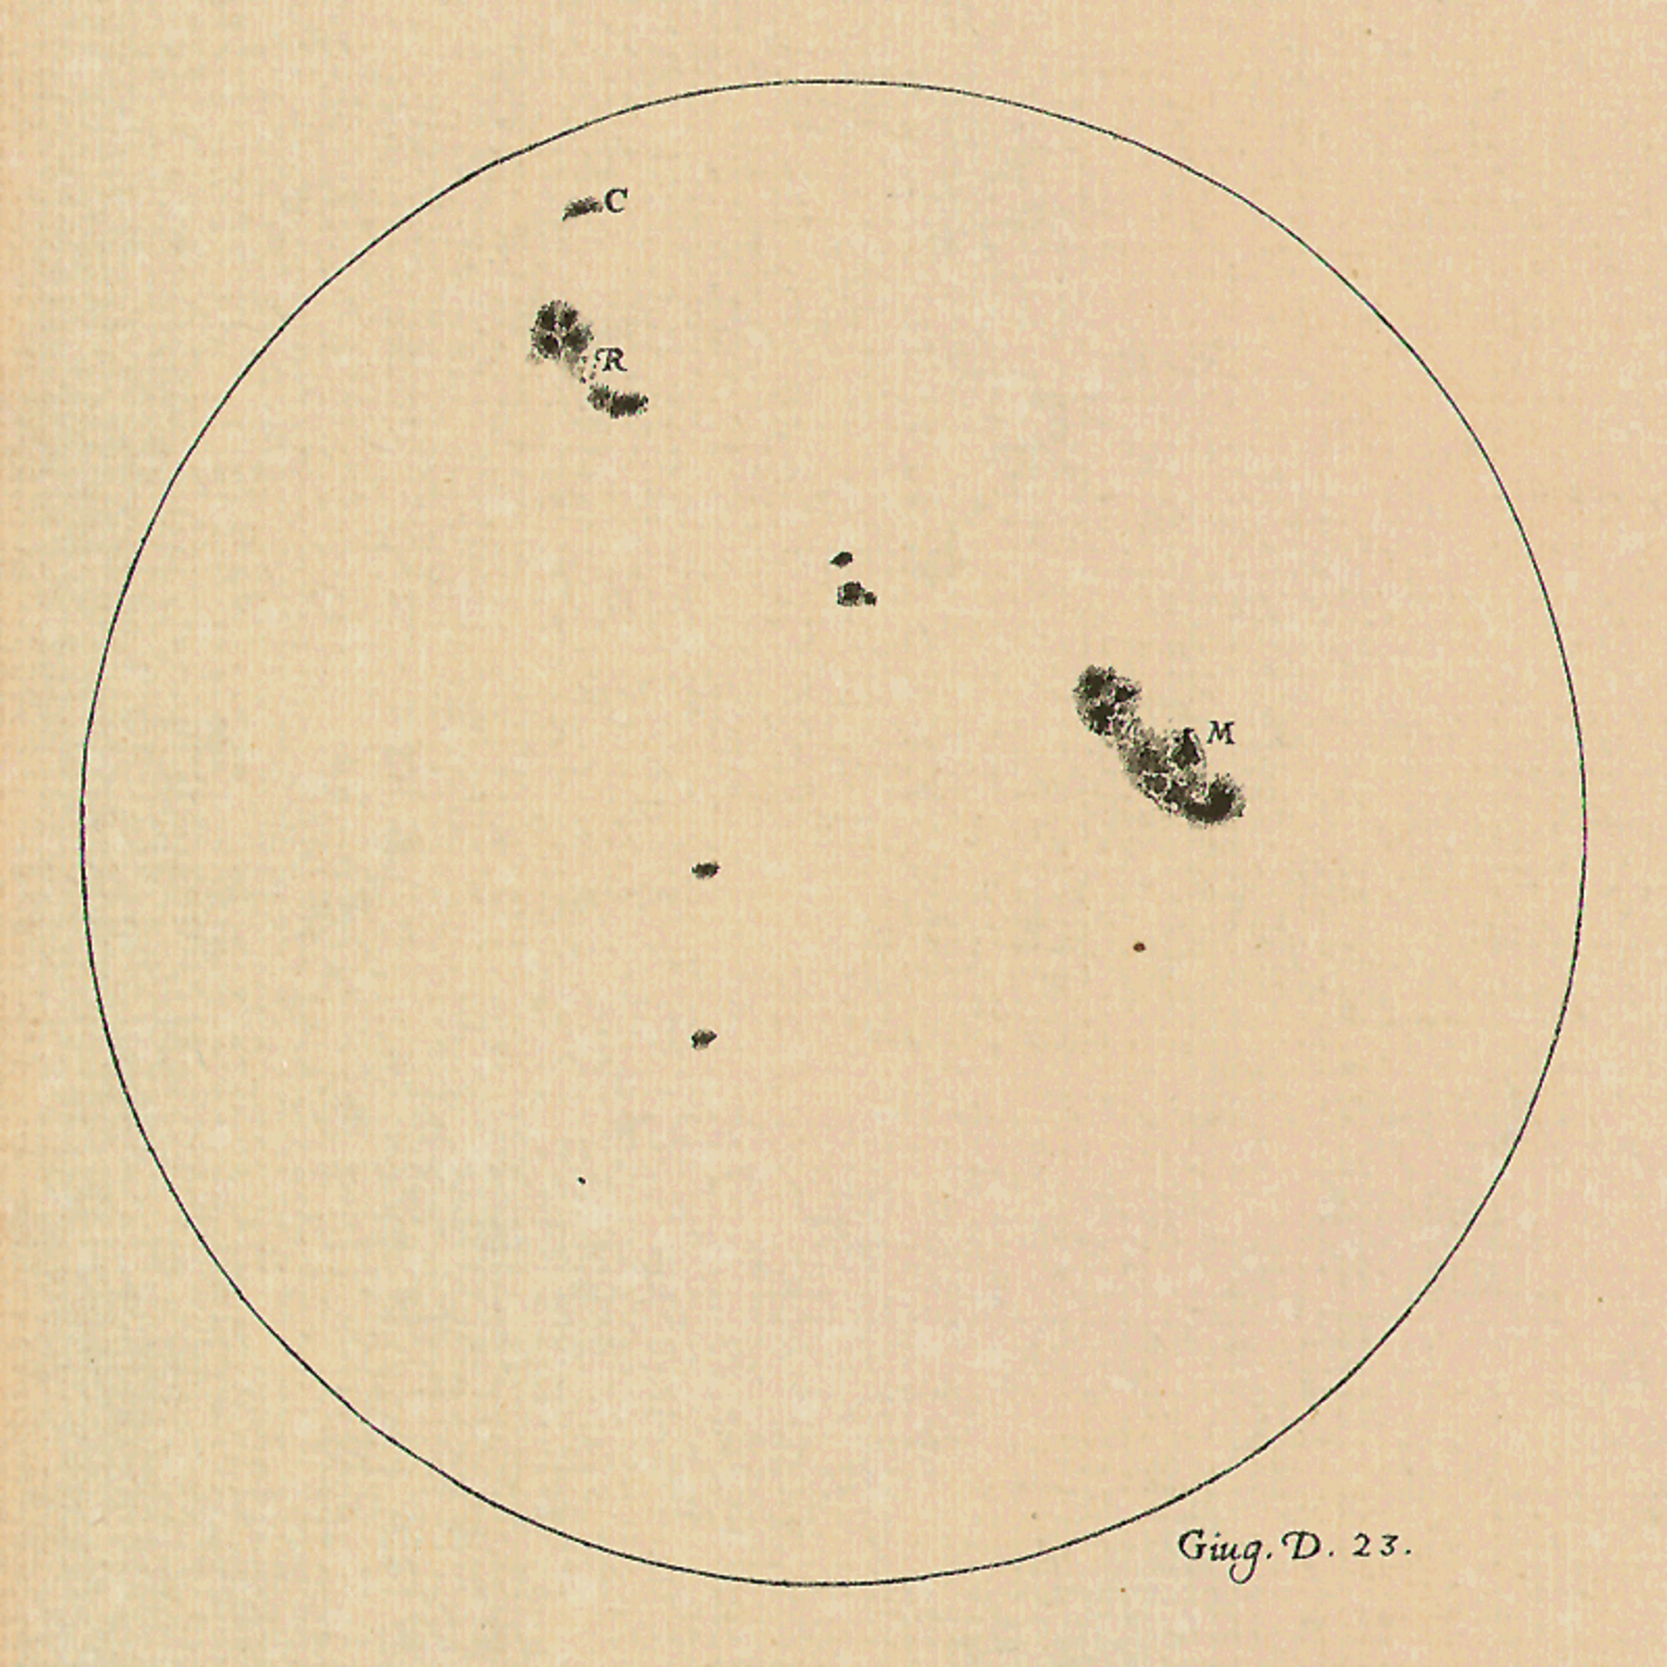
\includegraphics[width=\textwidth]{23_June_1613.pdf}
        \caption{
                 The creation of the telescope forever changed astronomy.
                 For example, here is a drawing of the solar surface by Galileo during the 17$^{{th}}$ century. 
                 Here, the sunspot structure can be resolved.
                 The inner (umbra) and outer (penumbra) regions can be seen clearly.
                 Image credit goes to \cite{galileo}.
               }
        \label{fig:galileo}
    \end{figure}
     
    Our local star is known as the Sun and is a semi-common and uninteresting main sequence star if you happen to be an astrophysicist.
    However to the general public and more importantly solar physicists, it forms the backbone of their lives.
    From simply as mundane as waking up at sunrise, to making a long and (hopefully) successful career in solar physics.
    
    For early humans, it was as a giant bright ball in the sky that appeared to revolve around the Earth and it defied any human understanding at that time.
    Since the dawn of mankind, the mythology surrounding the Sun has been numerous.    
    From the New World, the Aztec's had a sun god called Tonatiuh. 
    Without constant human sacrifice (mainly their enemies), they believed that the Sun would not move through the sky.
    From the Far East, the Chinese originally had 10 suns who took turns moving through the sky. 
    However, these suns were mischievous and decided to all appear at the same time. 
    This made life utterly unbearable on Earth, so an archer bestowed with a unique bow shot down 9 of the suns, leaving the one sun we have today.
    From the Old World, the Greeks and Romans believed in Apollo who is the son of Zeus and Leto.
    He was known as the god of music, healing, light, truth and the Sun; a very busy god.
    With the decline of polytheism and the rise of monotheism, these gods and stories quickly became consigned to history. 
    For a review of solar mythologies, see \citet{mythbook}.
    
    The Sun had always been observed with the naked eye, sunspots have been visible and recorded by the ancient Chinese, further, many solar calenders were created to order human society.
    However, no systematic studies of the Sun had ever taken place.
    It was until the enlightenment in Europe which marked the start of a massive transformation of European society, in which the telescope was invented (among other things).
    This is the beginning of modern astronomy.
    
    The telescope was the instrument that allowed humanity's knowledge of our solar system to radically change.
    It was possible to observe the Sun in much greater detail for the first time.
    Galileo drew many full disc images of the Sun and Figure \ref{fig:galileo} is one such example. 
    With the telescope, the umbra and penumbra of sunspots was easily differentiated for the first time.
    Further, pores can be seen in the image.
    From here, many other discoveries were made such as the sunspot cycle, differential rotation and solar flares.
    With more time and a solar eclipse, layers of the solar atmosphere were finally observed, such as the chromosphere and the corona.
    The age of solar physics had finally begun.
    
    The scientific understanding of the Sun has advanced by leaps and bounds, especially during the past sixty years.
    This is mainly due to the launch of space missions, whether it was SkyLab or the numerous satellites now pointed at the Sun.
    The removal of the Earth's atmosphere was a decisive step, allowing the observation of spectral lines not possible on Earth and vastly improving the quality of observational data.
    The solar physics community is hard at work analysing the massive amount of data that is available and expanding our knowledge of the Sun.   
    However, there are still crucial challenges to overcome.
    They have in essence become the holy grails of solar physics: how the corona is heated and what is the dynamo process behind the solar magnetic field.

\section{The structure of the solar interior}

    The Sun's internal structure is divided into four sections; the core, the radiative zone, the tachocline and the convective zone.
    While we cannot see these regions directly, the process of helioseismology, much like seismology on Earth, has allowed humanity to come to grips with these layers and processes that occur within the Sun.
    Figure \ref{fig:Sun} showcases the multi-layered structure of the Sun.
    The image starts from the core, through the various interior layers until it reaches the solar atmosphere and the interplanetary medium.
    This picture of the Sun has built up over time as our understanding has improved with the use of more observations and complex mathematical models during the past 100 years.
    
    \begin{sidewaysfigure}
        \centering
        \includegraphics[width=\textwidth]{sun.pdf}
        \caption{
                A schematic diagram of the interior and external layers of the Sun.
                Also shown are several features that occur within the solar atmosphere; sunspots, granulation, flares and prominences.
                Image credit to \cite{sun_image}.
               }
        \label{fig:Sun}
    \end{sidewaysfigure}

\subsection{The core}

    The core is the beating heart of the Sun, the largest fusion reactor this side of Centaurus.
    The core has more than 60\% of the total mass of the Sun and extends roughly to 25\% of the total radius of the Sun.
    It has a density of around 150000 kg m$^{-3}$ and a temperature around 16 MK \citep{0004-637X-699-2-1403}.
    The fusion reactions occur due to the high pressure and temperatures that exist in the core, which are enough to force the hydrogen atoms together. 
    This process, which accounts for the vast majority of the energy generated, creates a range of high energy particles such as photons and neutrinos.
    
\subsection{The radiative zone}

    Due to the intense heat and the large pressure within this region, thermal radiation is the only mechanism able to transfer the heat generated by the core.
    The process of radiative transfer within the radiative zone happens on very small scales.
    Photons are emitted and absorbed on very short time-scales. 
    This means that it takes hundreds of thousands years for photons to exit this layer.
    The radiative zone extends to about 70\% of the solar radius \citep{cox1991solar}. 
        
\subsection{The tachocline}

    The tachocline is the region that separates the radiative zone and the convective zone.
    It is very thin, its width being only 0.04\% of the solar radius.
    It has been long hypothesised that the solar magnetic field is created within this layer via a dynamo process \citep{stix2004sun,soward2005fluid}.

\subsection{The convection zone}

    From the tachocline, the temperature and pressure has decreased enough to allow the fully ionized molecules to retain some electrons and thus the opaqueness of the plasma increases.
    This traps part of the radiative energy from below setting up a temperature gradient sufficient enough to allow convection to take place.
    Thermal columns are created, which carry hot plasma to the surface of the Sun and once it cools, it sinks back to the base of the convection zone.
    This process is believed to cause gravity waves within the solar interior which have yet to be observed.
    The visible effect of convection is the solar granulation pattern that can be seen in white light images of the Sun.  
    The pattern consists of cells that have a rough hexagonal shape. 
    At the top of the convection zone, the temperature drops to 5700 K and the density to 0.0002 kg m$^{-3}$ \citep{gai2000sun}. 
    Within the convection zone, differential rotation is important.
    The Sun rotates not as a solid body as the Earth does but as a fluid as the Gas Giants do. 
    The rotation rate decreases from the equator where it is 25 days to around 34 days at the poles \citep{2000SoPh..191...47B}.
    Furthermore, the rotation rate varies with depth, until the tachocline is reached, where it rotates as a solid body \citep{Howe31032000}.
    
\section{The solar atmosphere}
 
    The solar atmosphere is quite unlike the Earth's.
    While they both have multiple layers, the characteristics are wildly different (as you would expect). 
    The top of the convection zone is the start of the first layer of the solar atmosphere.
    The reason for this is that the optical depth becomes $\lessapprox$1.
    The optical depth is defined as the fraction of photons that can pass through a layer without being scattered within that layer.
    For a value of $\lessapprox$1, this means that approximately a third of all photons will pass through this layer unhindered.
    This layer is called the photosphere.
    There are three more layers of the solar atmosphere: the chromosphere, the transition region and the corona (see Figure \ref{fig:Sun}).
    Then the solar atmosphere transitions into the solar wind which fills the interplanetary medium.
    
\subsection{The photosphere}

    The photosphere comes from the ancient Greek word ``photos'' meaning ``light''.
    It is the visible surface of the Sun, that can be seen with the naked eye.
    The photosphere has an approximate thickness of 500 km with a starting temperature of 5700 K which drops as you move away from the surface, getting to approximately 4500 K.
    This part is called the temperature minimum and is generally taken to be the top of the photosphere.

    The structure of the photosphere is composed of convection cells called granules, which are on average 1 Mm in diameter.
    Observed flows within these cells show uprising hot plasma in the centre which pushes the cooler plasma to the edges of the cell before flowing downwards. 
    These granules are short-lived, with a lifetime less than 10 minutes, resulting in a repeating pattern at small-scales.
    These can be seen in Figure \ref{fig:photosphere}, within circle A.
    On larger scales, super-granule structures have been observed with a 30 Mm diameter which can last for a day or longer \citep{lrsp-2010-2}.
   
    \begin{figure}    
    	\centering
    	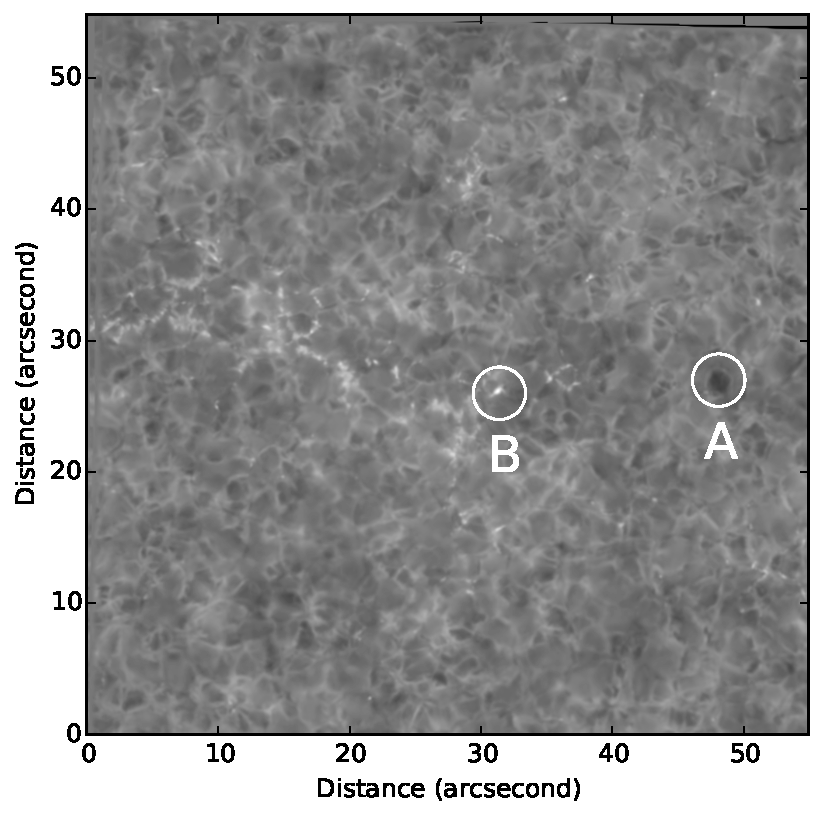
\includegraphics[width=\textwidth]{QS.pdf}
    	\caption{
    		Iron I ($630.2$ nm) image taken with the Swedish Solar Telescope on the $22^{{nd}}$ of July 2012.
    		It shows some of the features that are present in the quiet Sun: a granule cell (A) and a magnetic bright point (B).
    	}
    	\label{fig:photosphere}        
    \end{figure}   
       
    The convective nature of the Sun has allowed us to infer the interior structure. 
    The reason for this is that turbulence within the convection zone creates an entire spectrum of acoustic waves, named \textit{p}-modes, where \textit{p} stands for pressure.
    \textit{p}-modes penetrate into the solar interior and at certain frequencies, the waves become standing.
    These can be measured on the photosphere, using line-of-sight Doppler images. 
    The mathematics used as a basis for this research is called spherical harmonics and allows \textit{p}-modes that are observed to be understood.
    The mode's overall properties are affected by the physical conditions where the maximum amplitude for that mode occurs. 
    This allows an image to be built up at every depth within the solar interior.
    For reviews on this topic, see \cite{annurev.aa.22.090184.003113} and \cite{RevModPhys.74.1073} for example.
    
    The dynamics of the photosphere is governed by two processes, convection as discussed above, and the solar magnetic field.
    Thus understanding how the magnetic field is structured within the photosphere is important. 
    The most common method employed in solar physics to measure the magnetic field, is to exploit the Zeeman effect \citep{phillips1995guide}.
    When atoms are subjected to a magnetic field, their spectral lines split as a function of field strength and polarization.
    Unfortunately, this effect can only really be used in the photosphere as the magnetic field present is strong enough to cause the Zeeman effect.
    However, many solar physicists have attempted measurements in various weak field areas \citep{1995ApJ...439..474M,1538-4357-613-2-L177,2008A&A...489L..57K}.
    These images are called solar magnetograms and they have revealed the basic magnetic field structure at the photosphere.
    The magnetic field is very weak ($\le 40$ Gauss) on average and is very sparse \citep{0004-637X-636-1-496,2011A&A...526A..60V}.
    This is referred to as the quiet Sun and is shown in Figure \ref{fig:photosphere}. 
    The dominating feature within this image is the granulation cells, which is the structures formed by convection can be seen clearly as well as several small features, which are discussed below. 
    Since granulation can be seen clearly, the magnetic field does not dominate within the quiet Sun, as it does in other regions.
    
    Figure \ref{fig:valc} demonstrates the semi-empirical model of the quiet Sun atmosphere, where the density and temperature is blue and red, respectively \citep{1981ApJS...45..635V}.
    This model is termed the ``VALIIIc'' model and is used as the base atmosphere for many MHD simulations \citep{Mumford2015,GFME13a,fedun1,fedun2,2011AnGeo..29..883S,Wedemeyer2012,Vigeesh2012,0004-637X-743-1-14}.
    
    \begin{figure}    
       	\centering
       	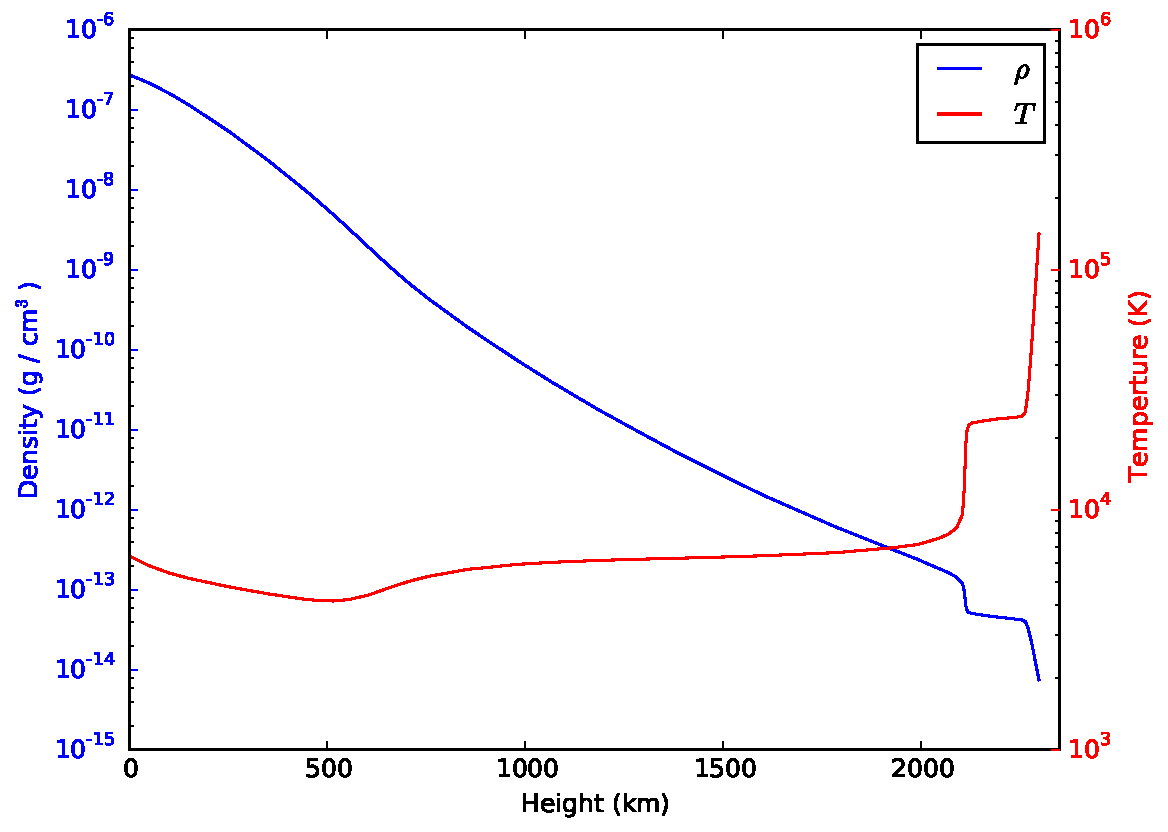
\includegraphics[width=\textwidth]{val3.pdf}
       	\caption{
       		     The VALIIIc \citep{1981ApJS...45..635V} model of the quiet Sun, density is blue and temperature is red.
       		     The temperature minimum region and the transition region can be seen clearly with these two parameters.
                 }
       	\label{fig:valc}        
    \end{figure} 
    
    Within the photosphere are small regions of concentrated magnetic field, named Magnetic Bright Points (MBPs).
    They are small-scale bright dots, as can be seen in Figure \ref{fig:photosphere}, in the circle labelled B.
    They are formed in the gaps between granule cells since the plasma flow drags the magnetic flux to high concentrations (>$1$ kG).
    The most likely reason for the increased brightness is that the flux tube has been evacuated of plasma.
    As such, observations of MBPs allow a glimpse into the top of the convection zone, which has a higher temperature than the photosphere and is brighter.
    One important factor about MBPs was the observation of Alfv\'en waves \citep{Jess2009,Taroyan2009}.
    This was able to supply enough energy to the corona to overcome the ``Coronal Heating problem'' (detailed in section \ref{corona}).
    
\subsubsection{Active regions}
    
    Active Regions (ARs), sometimes referred as sunspot groups, are areas of intense magnetic field concentrations located on the Sun's surface.
    They are catalogued by the National Oceanic and Atmospheric Administration (NOAA) who assign each AR an identification number.
    ARs vary in scale, lifetime and what magnetic structures are present and two of most prevalent features within ARs are sunspots and pores.
    Furthermore, most ARs will contain magnetic features found in the quiet Sun and events that are believed to be a consequence of magnetic reconnection.
    This events are more likely to occur within ARs due to the more complex magnetic field geometry.
    Figure \ref{fig:AR} displays an AR and it consists of 3 sunspots, taken as the AR is about to disappear off-limb.
    Circle A encloses one of the sunspots, but by use of a different wavelength filter we can observe an EB (B) and a jet event (C).
    The last two events are associated with magnetic reconnection \citep{2013SoPh..283..307N,2013A&A...560A..31N,2013ApJ...779..125N,2015ApJ...798...19N}.
     
    \begin{figure}
        \centering
        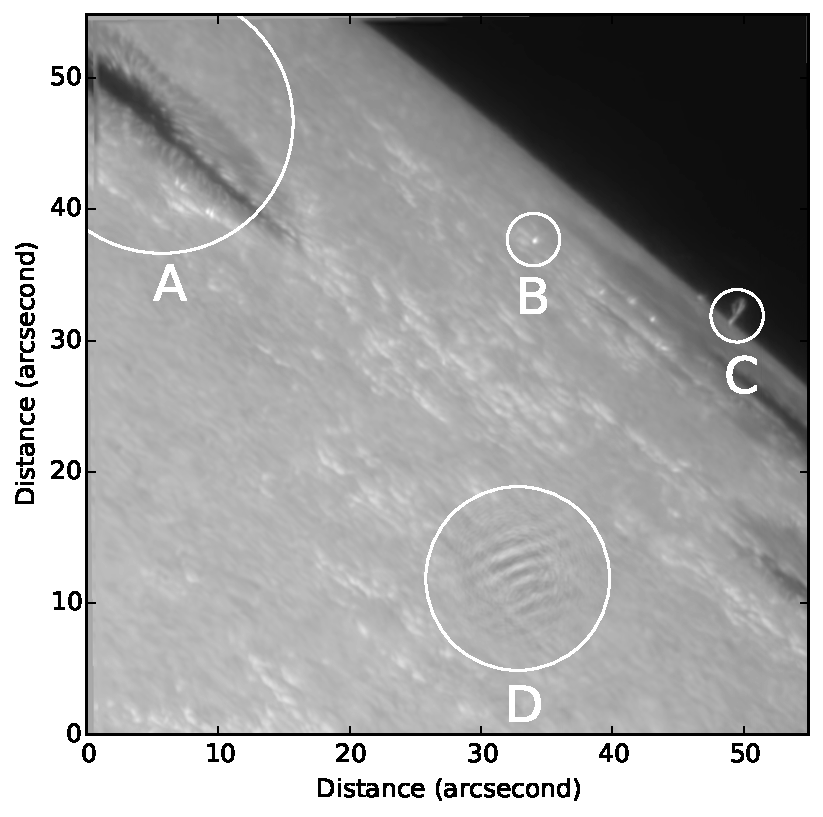
\includegraphics[width=\textwidth]{AR.pdf}
        \caption{
                 An image of an active region (NOAA 11504) sunspot taken with the Swedish Solar Telescope using the Crisp Imaging SpectroPolarimeter on the $21^{{st}}$ June. 
                 The H$\alpha$ filter is used but into the far wings, such that strong photospheric features can be observed.
                 It shows some of the features that are present in Active Regions; sunspot (A), Ellerman Bomb (B), a jet (C) and seeing effects (D).
                }
        \label{fig:AR}
     \end{figure}    

	ARs will form within a band from the equator, typically $\pm$30$^\circ$ and arise from a large flux bundle that is formed deep in the convective zone \citep{SAO,1974MNRAS.169...35M,2014SoPh..289.3351T}.
	Magnetic buoyancy is the reason this bundle rises as a $\Omega$-shaped loop that breaks through the photosphere.
	On small scales, the magnetic field is fragmented and convection concentrates the emerging magnetic flux such that intense magnetic flux tubes form.
	Figure \ref{fig:dynamo_field} shows a schematic of how the magnetic flux is transported upwards to form ARs.
	The process requires two processes: the solar dynamo to create the magnetic field and differential rotation to create the flux bundle.
	Typically, it can take up to 4 days for the AR to form completely and it is common that a cluster of sunspots are surrounded by regions of enhanced brightness in the photosphere and in the corona, EUV and X-ray loops can be seen to be anchored in ARs \citep{2014masu.book.....P}.
	An AR can reach its maximum size in two weeks and sunspots will keep forming as long as magnetic flux emerges but most sunspots will decay after a single rotation.
	The leading sunspot in an AR is called the p-spot or leader and the last sunspot in the AR is called the f-spot or follower.
	It is common that the leader sunspot is long-lived while the follower sunspot will short-lived, be irregular in shape and an opposite polarity magnetic field to the leader sunspot.
	
	\begin{figure}
		\centering
		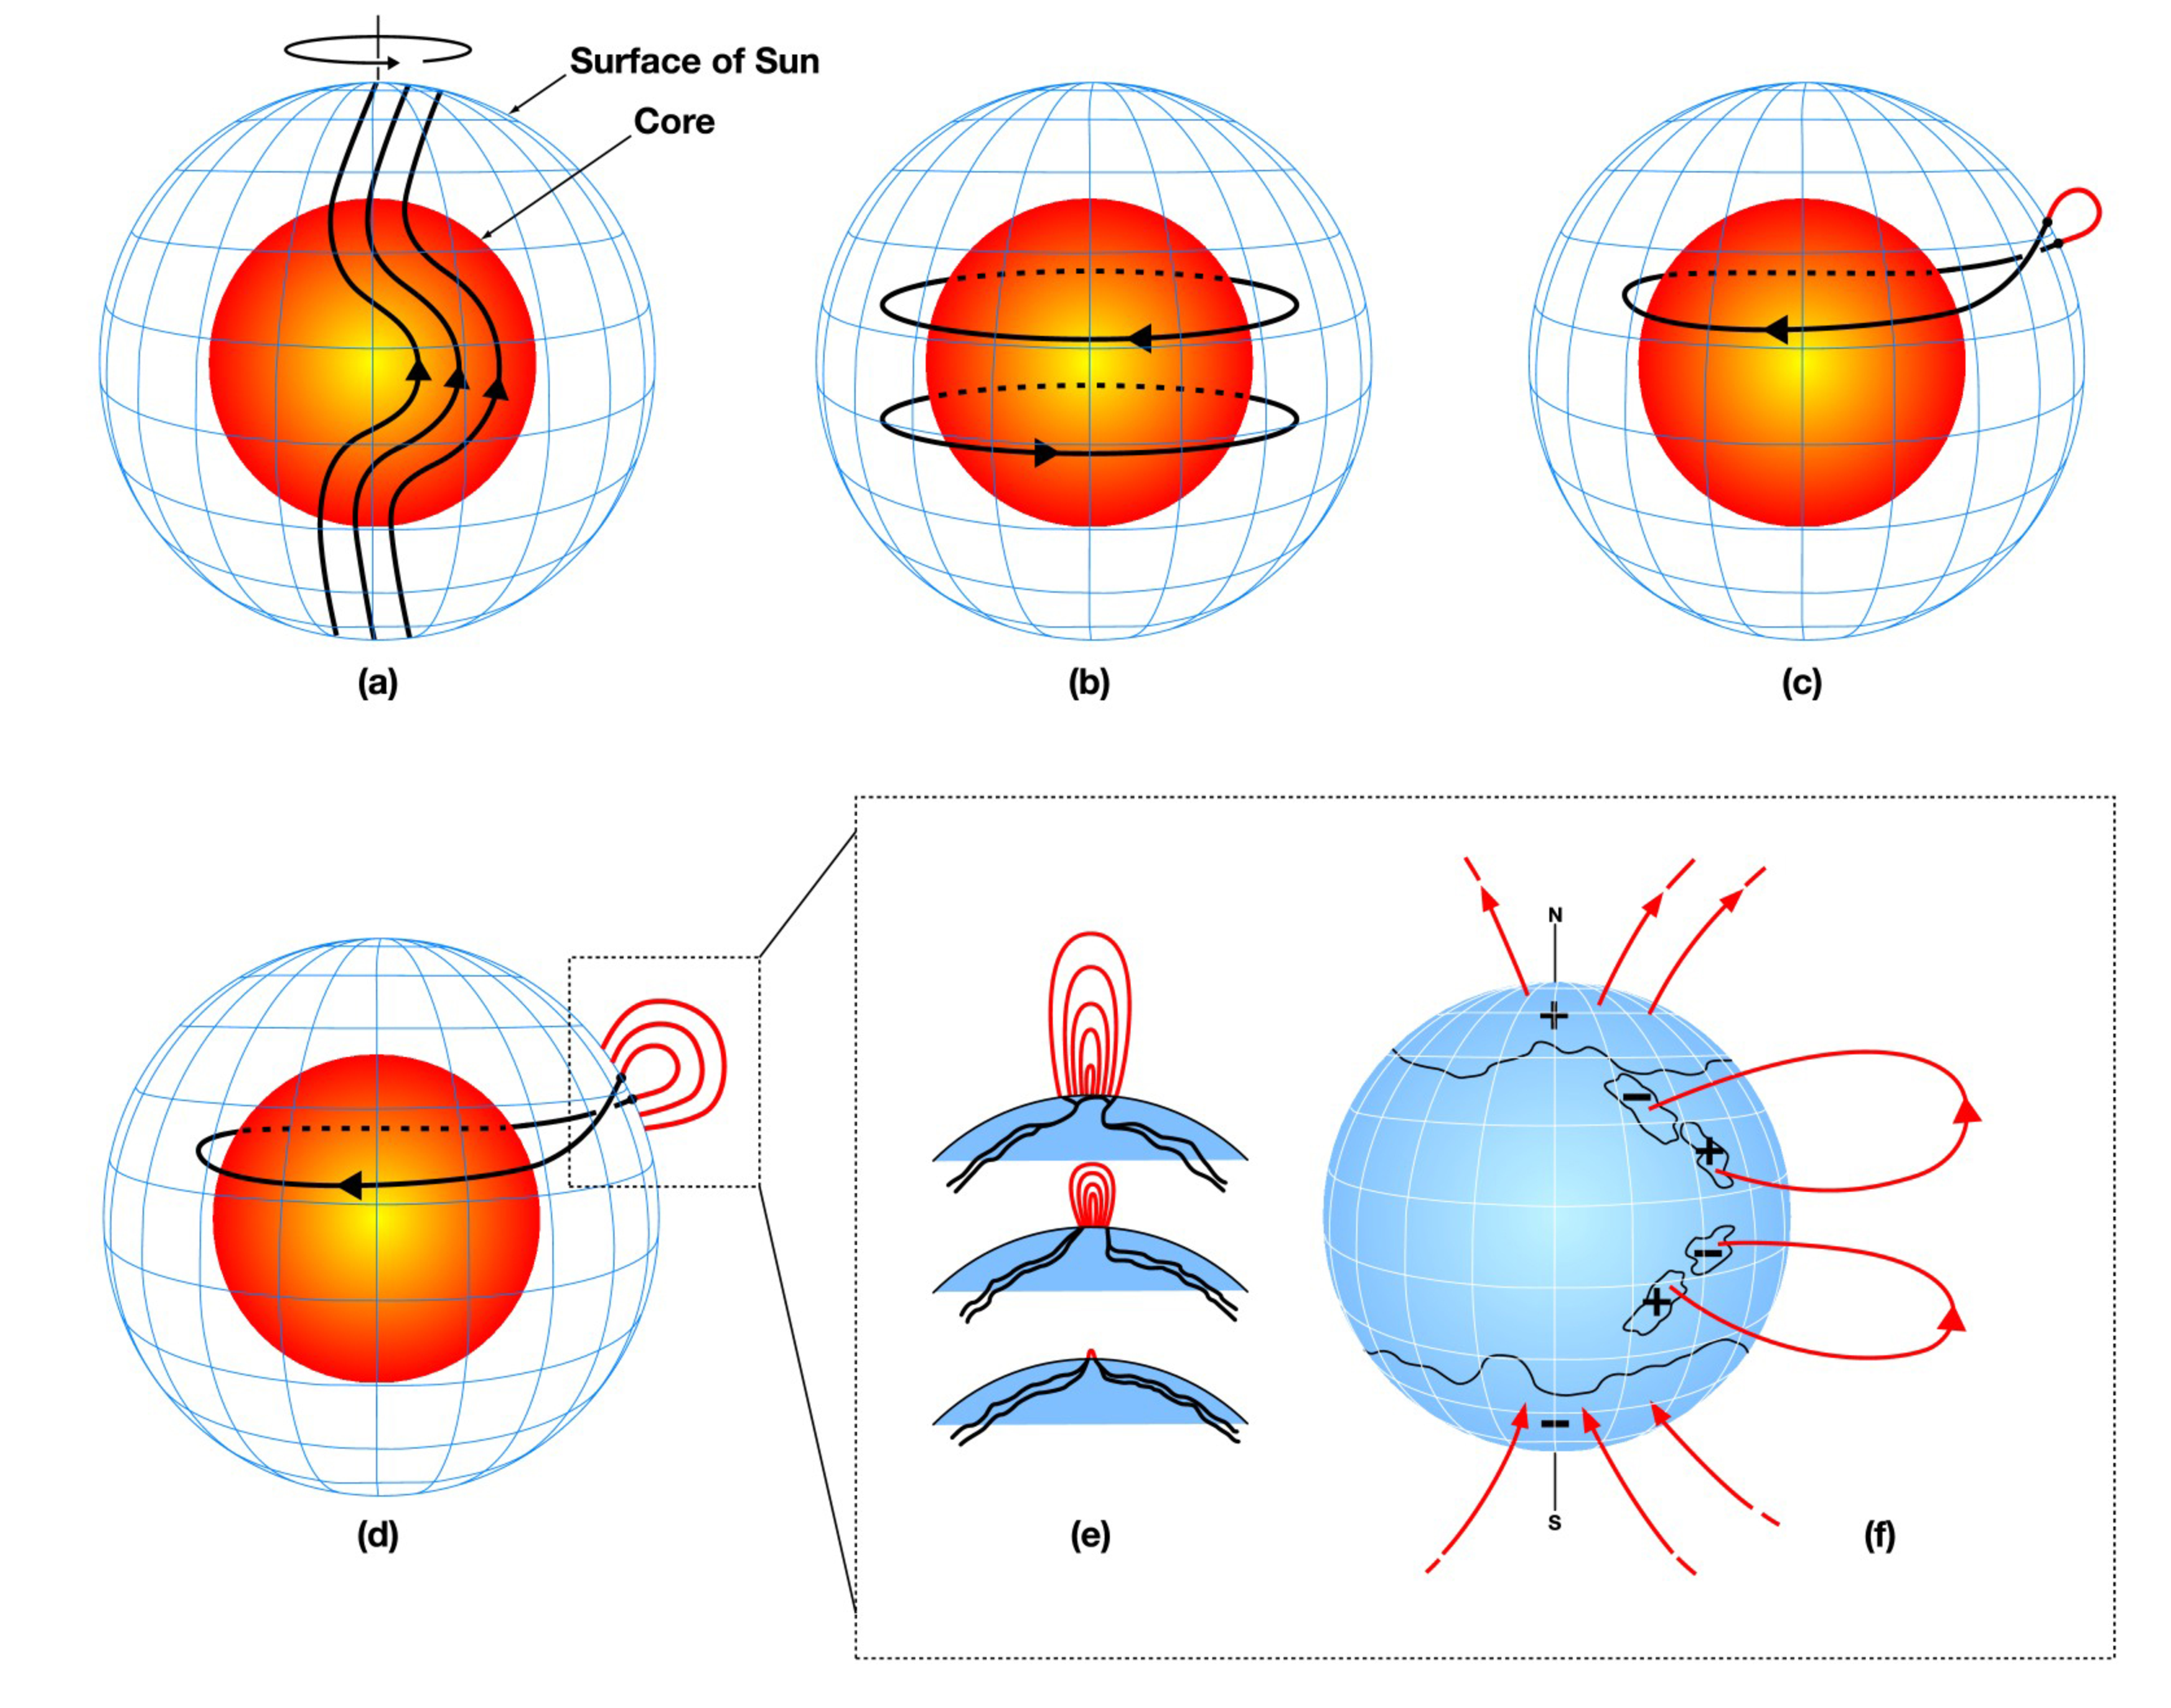
\includegraphics[width=\textwidth]{dynamo.pdf}
		\caption{
				 Schematic of magnetic flux emergance.
				 The red inner sphere represents the Sun's radiative zone and the blue mesh the photosphere and the solar dynamo is between these two layers
				 (a) The Sun's differential rotation shears the magnetic field.
				 (b) Toroidal magnetic field is produced due to differential rotation.
				 (c) Buoyant magnetic loops rise to the surface when the magnetic field is strong enough and they twist as they rise due to differential rotation.
				 Sunspots are formed from these loops.
				 (d,e) Additional magnetic flux emerges. 
				 (f) Magnetic flux spreads in latitude and longitude from decaying sunspots.
			     Reproduced from \cite{1367-2630-9-8-297} and is available online from \url{http://www.arrl.org/w1aw-bulletins-archive/ARLP018/2013}.
		        }
		\label{fig:dynamo_field}
	\end{figure}
			
	ARs are classified by the magnetic field polarity of the entire region is as follows.
	A unipolar ($\alpha$-type) AR make up 46\% of all ARs while a bipolar ($\beta$-type) AR makes up 53\% and the remaining ARs have a complex ($\gamma$-type) magnetic polarity \citep{2014masu.book.....P}.
	Figure \ref{fig:AR_Mag} show a complex AR that was observed with the National Aeronautics and Space Administration's (NASA) Solar Dynamics Observatory's (SDO) Helioseismic and Magnetic Imager (HMI) instrument.
	The top image is a white light view of the AR while the bottom image is a line-of-sight (LOS) magnetogram where blue is positive polarity and red is negative polarity.
	ARs with complex magnetic field geometries are more likely to be the source of a large solar flare.
	Furthermore, $\delta$-type sunspots have an umbra that has opposite polarity to penumbra.
	Sunspots move faster than the surrounding local plasma and this implies that they are anchored below the surface where the rotation rate is faster.
	ARs tend to drift apart at a rate of 0.1$^\degree$ per day due to the leader sunspot being at a lower latitude.
	
	\begin{figure}
		\centering
		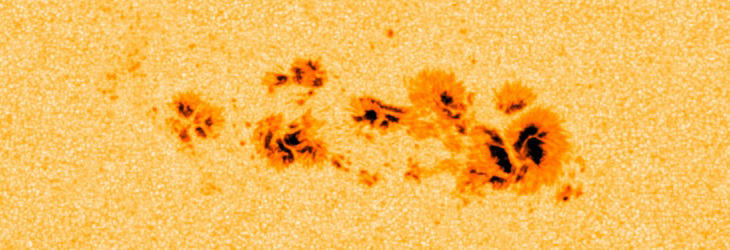
\includegraphics[width=\textwidth]{sunspot.jpg}\\
		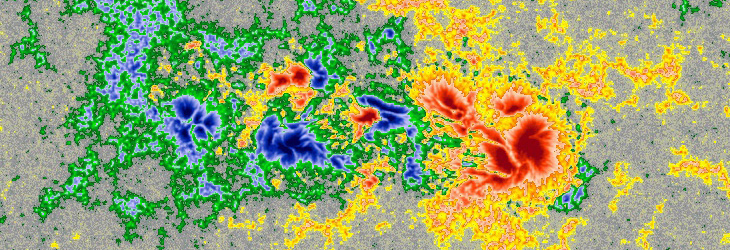
\includegraphics[width=\textwidth]{sunspot_magnetic.jpg}\\
		\caption{
			     An example of a complex AR as seen by National Aeronautics and Space Administration's (NASA) Solar Dynamics Observatory (SDO)'s Helioseismic and Magnetic Imager (HMI) instrument.
			     The top image is the AR as seen in white light.
			     The bottom image is a magnetogram and displays the line-of-sight (LOS) magnetic field of a AR where blue indicates positive polarity and red indicates negative polarity.
			     Taken from \url{http://www.spaceweatherlive.com/en/help/the-magnetic-classification-of-sunspots}.	
		        }
		\label{fig:AR_Mag}
	\end{figure}
		
\subsubsection{Sunspots}

    Sunspots are the strongest magnetic field concentrations on the solar surface.
    The historical account of sunspots starts in a chronicle by John of Worcester in 1128.
    With the invention of the telescope sunspots had been resolved into two parts by Galileo and Christoph Scheiner and they showed that sunspots lie near the solar equator.
    At the solar limb, Alexander Wilson noticed that the penumbra that is farthest from the limb is narrower he deduced that sunspots are on the surface of a moving sphere. 
    Furthermore, he deduced that a sunspot is a saucer-like depression (500-700 km) in the visible surface and this was named the Wilson effect.
    It was due to the colder, less-dense umbra being more transparent such that umbral light comes from a deeper level than the normal photosphere \citep{2014masu.book.....P}.

	With the naked eye, sunspots appear as dark spots on the solar surface.
	The reason for this darkness is due to the partial inhibition by the sunspot's magnetic field of convection, which is the dominate process that transports energy in the convection zone.
	However, with a telescope, a sunspot can be divided into two regions.
	The first is the umbra with an almost vertical magnetic field which is surrounded by a brighter and penumbra with a weaker more horizontal inclined magnetic field.
	The penumbra is highly filamentary which has a pattern of bright and dark radial filaments.
	The umbral radius can make up to 50\% of the total sunspot radius.
	The brightness of the sunspot is dependant on wavelength but the total brightness (integrated over all wavelengths) is around 30\% of the quiet Sun.
	The temperature is 1000-2000 K less than the quiet Sun photosphere which implies that a substantial convective flux is required to maintain this brightness.
	The penumbra radiates 75-85\% of the quiet Sun photosphere and is only cooler by up to 400 K.
	Sunspots come in a range of shapes and sizes, with typical diamters that are 3.5 to 60 Mm and it was discovered that the lifetime of a sunspot is proportional to its area. 
	For example, a sunspot with diameter of 10 Mm will live for 2-3 days while a sunspot with a 60 Mm diameter will live up to 80-90 days.
	
	The magnetic field in the centre of the sunspot umbra is vertical and its strength increase while its brightness decreases with respect to size.
	The mean umbral magnetic field strength is 2.8 kG while it can be as weak er 1.5 kG and as strong as 6kG \citep{2006SoPh..239...41L}.
	The magnetic field strength decreases gradually with increasing radius from the centre and an average magnetic field over the entire sunspot is 1.2-1.7 kG.
	The penumbral inclination of the magnetic field increases with radius to a mean value of 70-80 degrees at the edge of the sunspot and the magnetic field weakens to 700-900 G.

	The umbra of a sunspot is far from uniform.
	It is known that dark nuclei that are around 15\% brightness of the quiet Sun photosphere with diameters up to 1Mm are located within the umbra.
	Furthermore, umbral dots are small bright features that are found in all sunspots and pores, \cite{1950Obs....70..234T,1964ApJ...139...45D}.
	They have diameters range of 100-450 km, they are associated with upflows of \textasciitilde1 km s$^{-1}$ and lifetime of 10 minutes to 2 hours \citep{1997A&A...328..682S,1997A&A...328..689S}.
	They used to be called umbra granulation before the range of high-resolution imaging possible now.
	While they only cover 3-10\% of the umbra, they account for 10-20\% of the brightness and about 1000 K hotter than the normal umbral atmosphere.
	Light-bridges are narrow bright features (similar to penumbral brightness) that cross over the umbra of a sunspot or pore.
	Essentially, a light-bridge is a fissure separating two different components of a sunspot and in this fissure is a dark lane that is an enhancement of density.
	They are typically seen before the breakup and fragmentation of a sunspot as they can continue to grow in size during the decay of a sunspot.
	
	The penumbra of a sunspot is made up of filaments which are 3.5-7Mm long and on average can last for 0.5-6 hours.
	There are two types of penumbral filaments: Bright filaments and dark filaments.
	The bright filaments are around 95\% of the brightness of the photosphere while the dark filaments are 60\% brightnesses.
	Filament widths are around 150 km and posses unresolved features below current spatial resolution available with solar telescopes \citep{2002Natur.420..151S,2011Sci...333..316S}.
	
	The magnetic field of the penumbra is described as a interlocking comb.
	The magnetic field is more horizontal in dark filaments than bright filaments.
	There can be considered to be three components to the penumbral magnetic field \citep{2005A&A...436.1087L}.
	First, the bright filaments are more vertical and form loops extending for large distances from the sunspot.
	Some dark filaments make up a shallow canopy about 300 km high and reach twice the sunspot radius \cite{1991A&A...252..821D}.
	Other dark filaments bend lower over and dip below the surface of the penumbra (CHECK) \citep{1993ApJ...403..780T}.
	The overall structure evolves with time and it can interact with neighbouring magnetic field that are inclined which leads to magnetic reconnection and fine-scale penumbral jets.
	It should be noted that it has been argued that dark and bright filaments are not separate categories of filaments \citep{2013A&A...557A..25T}.
	
	The most well known flow associated with a sunspot is called the Evershed flow.
	It is a radial penumbral outflow in the photosphere that is parallel to the magnetic field.
	The average velocity is 2.5 km s$^{-1}$ but if the flow can be isolated in the observation, it as high as 6 km s$^{-1}$ \citep{2003A&A...403L..47B}.
	The flow is horizontal with a upwards inclination and a downwards inclination of 15 and 5 degrees in the inner and outer penumbra \citep{2004A&A...415..717T}.
	As the flow is observed in increasing height, it slows and reverse direction in the chromosphere.
	This is called the Evershed inflow or reserve Evershed effect and it extends over a fairly large region surrounding the sunspot and can be observed to occur along large fibrils.
	
    pores can be considered as smaller scale sunspots without a penumbra and thus are sometimes referred to, as ``naked umbra'' sunspots.
    They are intermediate flux concentrations between normal intensity flux tubes and sunspots.
	pores have diameters that range from 0.7 to 7 Mm and the largest are bigger than the smallest sunspots.
	When compared to sunspots, they have a brightness that is 50\% of the quiet Sun photosphere and a central magnetic field strength of 1.8-2.3 kG and at the edge it has dropped to 1 kG.
    Due to their small size, pores have not been studied as much as sunspots since it took a new generation of solar telescopes in order to resolve them clearly.
    One example of a pore can be seen in Figure \ref{fig:chromosphere}, which is studied in Chapter \ref{chapter5}.
    This image is in the H$\alpha$ core which samples the chromosphere which is discussed in the next section.

    \begin{figure}
    	\centering
    	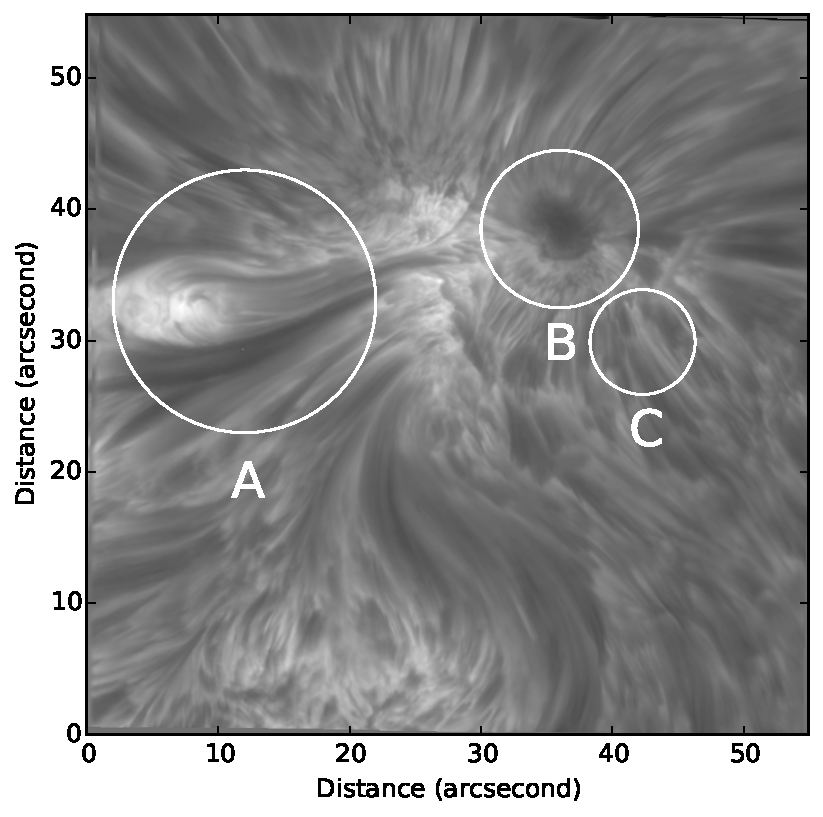
\includegraphics[width=\textwidth]{Chromo.pdf}
    	\caption{
    		A H$\alpha$ line core image of Active Region NOAA 11510 observed on the 22$^{{nd}}$ June 2012.
    		Here, this AR has a large pore that displays Running Penumbral waves (the focus of Chapter \ref{chapter5}).
    		Highlighted here are fibrils (A), the pore (B) and dynamic fibrils (C).
    		The complex nature of the chromosphere can be seen in detail and it still needs a full explanation.
    	}
    	\label{fig:chromosphere}
    \end{figure}   
    	
    Sunspot formation is a hotly debated topic (as many things are in solar physics).
    One current hypothesis about their formation is as follows.
    The magnetic field of the Sun, created by the solar dynamo, is strongly polarised and with differential rotation, these magnetic fields lines become bunched together, increasing the local magnetic field strength.
    This effect creates a buoyancy force which slowly makes this newly created flux region rise towards the surface until it penetrates into the photosphere.
    The flux tube that is buoyed upwards has an $\Omega$-shaped loop and field strength $>$1000 G \citep{stix2004sun,2014SoPh..289.3351T}.
    The strong magnetic field stops overturning convection which means that the plasma in this flux tube cools and falls. 
    The magnetic field will grow until the external gas pressure is balanced with the internal magnetic pressure.
    As the sunspot or pore forms, an annular convection cell, referred to as a moat is formed around the flux tube and can be considered a super-granular cell with a sunspot in the middle.
    This moat has up flow at the flux tube and a horizontal flow at the boundary of the flux tube and further out.
    
    Furthermore, sunspots can be formed by the accumulation of magnetic flux which collects at the boundary of a super-granule cell or a junction of several cells \cite{1974MNRAS.169...35M}.
    pores can appear if there is a down flows of 0.5 km s$^{-1}$, and cooling signals the onset of convective collapse.
    These pores last for hours or a day at most but it if keeps growing, it can form into a small sunspot with the diameter of 3.5-7 Mm and 1x10-20 MX such that a penumbra appears \citep{2010A&A...512L...1S}.
    Smaller sunspots will fragment within a few days after a light-bridge forms across part of the umbra.
    It is common to see light-bridges form along the boundaries between pores that coalesced to form the sunspot.
    Long lived sunspots decay very gradually as the area shrinks in size at a constant rate as magnetic flux is carried away by the outwards flows around a sunspot which gets cancelled in the photosphere \citep{2002AN....323..342M,2008ApJ...686.1447K}.
                          
    It should be noted, however, that a complete understanding of how sunspots form has not yet been achieved and the mechanism is likely to be more complex than the one described above.
    A more thorough review of the formation, evolution and unanswered questions relating to sunspots can be found these reviews, \cite{SAO,2008sust.book.....T,lrsp-2011-3}.

    While sunspots have been under near constant observation for several centuries.
    It was not until the mid 20$^{{th}}$ century, that oscillations were observed within sunspots themselves \citep{OASO}.
    There are three main sunspot phenomena: 3-minute (5 mHz) and 5-minute (3 mHz) oscillations and running penumbral waves (RPWs).
    The first two are observed with a LOS analysis, i.e., frequency filtering using the Fast Fourier Transform (FFT) (which is covered in Chapter 2).
    However, there is some evidence to suggest the existence of longer period oscillations \citep{LPO,SOS,Chorley2011}.
    The source of the 5-minute oscillation is thought to be a result of forcing by the 5-minute \textit{p}-mode global solar oscillation \citep{OWS,WAUO}.
    The 5-minute oscillation are typically seen in lines which form low in the cool umbral photosphere and are moderately suppressed not only in the penumbra, but also in the chromospheric atmosphere above the umbra \citep{OASO}.
    The cause of the 3-minute oscillation is still unknown but there are two main theories: they are either standing acoustic waves which are linked to the resonant modes of the sunspot, or, they are low-$\beta$ slow magneto-acoustic waves guided along the ambient magnetic field \citep{UTMO,OWS,OASO,ORWS}.
    The 3-minute oscillation are seen in elements that form higher up, in the low chromosphere, and these are also moderately suppressed in the penumbra \citep{OASO}.
    However, it should not be assumed that the period of these waves form one finite peak in a power spectrum; generally, the immediate spectral area around these periods has several peaks clustered tightly together.
	\textbf{The 3-minute oscillation is non-linear and compressive and at their peak intensities create sudden brightening called umbral flashes in chromospheric lines such as \ion{Ca}{K} and \ion{H}{$\alpha$} \citep{1969SoPh....7..351B}.
    The flashes have a rapid increase and slow decrease in brightness, the have a periodicity of 140-190 seconds and diameters up to 2 Mm and move rapidly towards the penumbra at speeds of 40 km s$^{-1}$ \citep{2003A&A...403..277R}}
    A review of sunspot oscillations can be found in \cite{OASO} and a review of solar oscillations can be found in \cite{SO}.
    
    The solar cycle is on average a 11-year variation that the Sun undergoes.
    This cycle manifests itself as a variation in the number of sunspots, the amount of solar irradiance and the levels of other solar activity \citep{climate}.
    The polarity of the solar magnetic field inverts as well.
    So some suggest that the full solar cycle is 22 years, but the features that occur on the Sun seem to be independent of the current magnetic field polarity. 
    Each cycle has a solar maximum and a solar minimum.
    A solar maximum and a solar minimum refer to periods of maximum and minimum sunspot counts, respectively and cycles span from one minimum to the next.
    As the names suggest, there is a large amount of ARs and magnetic activity at a solar maximum, while this is reduced in a solar minimum.
    Each solar cycle can be seen in the amount of sunspots which are visible (i.e., the amount of ARs that form).
    This has been counted since the 17$^{{th}}$ century and it is called the sunspot number catalogue \citep{Eddy18061976}.
    Figure \ref{fig:AR_Num} displays this catalogue with the raw count as the blue line and a running average in red.
    The main conclusion is that each cycle has a different duration and will produce a differing amount of sunspots.
    Since each solar cycle will differ in strength, the variation in the number of ``extreme'' events, such as flares and coronal mass ejections (CMEs) is observed.
    The reason is that these events require regions of strong magnetic field concentrations, i.e., ARs.
    So as the number of ARs decline, the possible regions that can cause flares or CMEs also decreases.
    Finally, the structure of the solar atmosphere will vary during each solar cycle as the magnetic field has an important effect on how the solar atmosphere is structured \citep{Sven}. 

    \begin{figure}
    	\centering
    	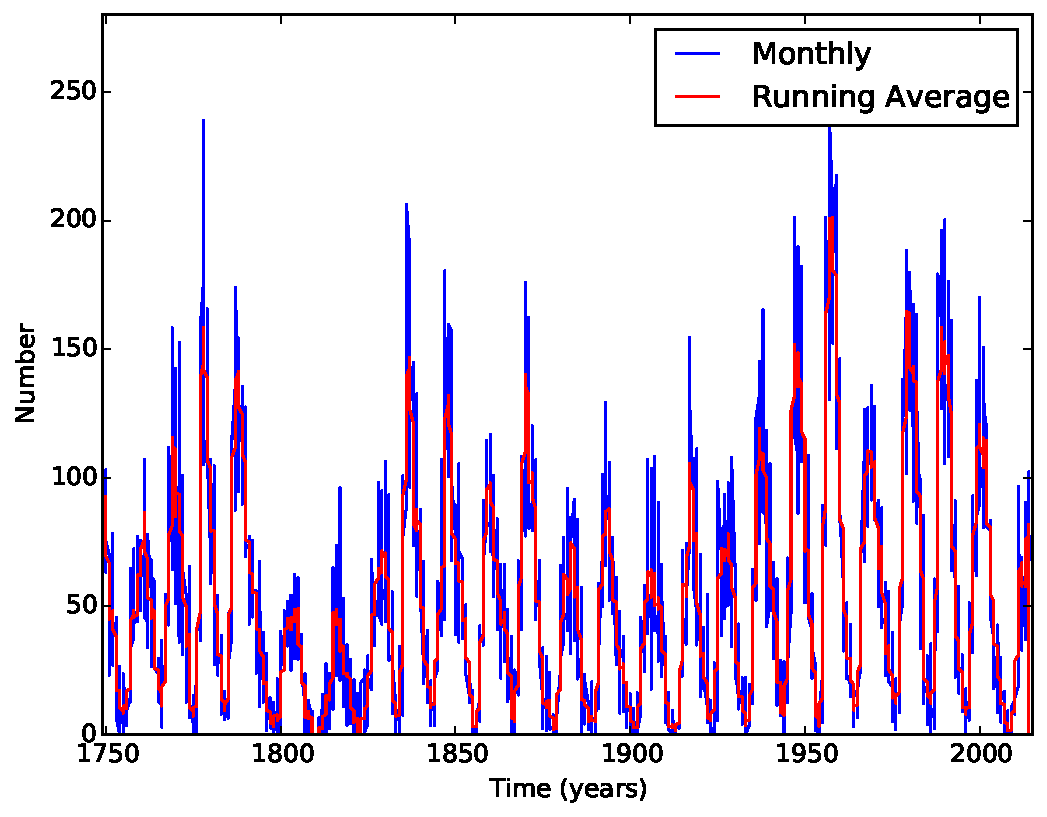
\includegraphics[width=\textwidth]{sunspot_number.pdf}
    	\caption{
	    		 The sunspot number record as it currently stands since continuous observations.  
    		     The eleven year solar cycle is clearly visible.
    	        }
    	\label{fig:AR_Num}
    \end{figure}   
            
    The solar cycle can directly impact the Earth's climate, as shown by the Maunder Minimum, which was an abnormally low amount of sunspots during the late seventeenth century and was the suspected cause of the Little Ice Age \citep{FRIIS-CHRISTENSEN01111991,climate}.
    Earth, over the past five years was seeing another abnormal solar minimum, though it was not on the scale of the Maunder Minimum, it still had some effects on the climate.
    This was evidenced by the recent cold winters experienced by the northern hemisphere and it could influence the relationship between the atmospheric oscillations which affect the temperature of the northern hemisphere \citep{CWE,NAO,SCR}. 
   
\subsection{The chromosphere}
\label{chromo}

    The next layer is visible from Earth when there is a total eclipse of the Sun, it is seen as an intense red region which got it the name, the chromosphere, from the Greek word ``chroma'', meaning colour.
    It is roughly $2$ Mm thick and is a highly complex layer.
    The temperature of the chromosphere increases with height and reaches around $20,000$ K at the boundary where it meets the next layer, the transition region.    
    The chromosphere is host to many small-scale structures that have been discovered due to the increasing optical resolution of solar telescopes over the past few decades.
    To observe the chromosphere from Earth, it is common to use either a H$\alpha$ filter, or a Ca II filter. 
    These are discussed in more detail later on in Chapter 2. 
        
    There are various names for these small-scale structures: spicules, fibrils, mottles and straws.
    The prevailing hypothesis is that there are two spicule types.
    Type I spicules are mainly seen in ARs but are scattered loosely elsewhere in the solar atmosphere.
    They can reach speeds up to $50$ km s$^{-1}$ and heights of $5$ Mm before falling back down, with typical lifetimes of $3$ to $10$ minutes, diameters of $120$ to $700$ km and temperatures of $10$ to $15$ kK.
    On disc, they are called dynamic fibrils and called mottles in the quiet Sun.
    Fibrils tend to be more elongated than mottles which are shorter.
    
    Type II spicules are located more often in the quiet Sun.
    They are faster (up to $150$ km s$^-1$), longer (up to $10$ Mm) and have a significantly reduced lifespan (up to $150$ s) when compared to Type I spicules.
    On disc, they are referred to as straws or more commonly Rapid Blue-shift Events (RBEs) \citep{Zaqarashvili2009}.
    Finally there is another fibril type that are long and mostly horizontal and longer-lived than dynamic fibrils.
    Some of these features are highlighted in Figure \ref{fig:chromosphere}.
    The circle A, has a good example of fibrils, long and fairly static, while circle C, shows dynamic fibrils which continually moved and swayed under our observation.
    
    These structures have been under investigation as a potential source of energy transport in the solar chromosphere.
    \cite{Morton2012} using ground-based observations discovered incompressible transversal motions for fibrils which match the ones observed for limb spicules which were interpreted as Alfv\'en waves \citep{DePontieu2007}.
    Further, fast compressive MHD waves were also observed.
    The estimation of the energy these waves carry is quite large but explaining how they dissipate this energy is unknown at this time.
    A review of oscillations in spicules can be found by \cite{Zaqarashvili2009}. 

    \begin{sidewaysfigure}
    	\centering
    	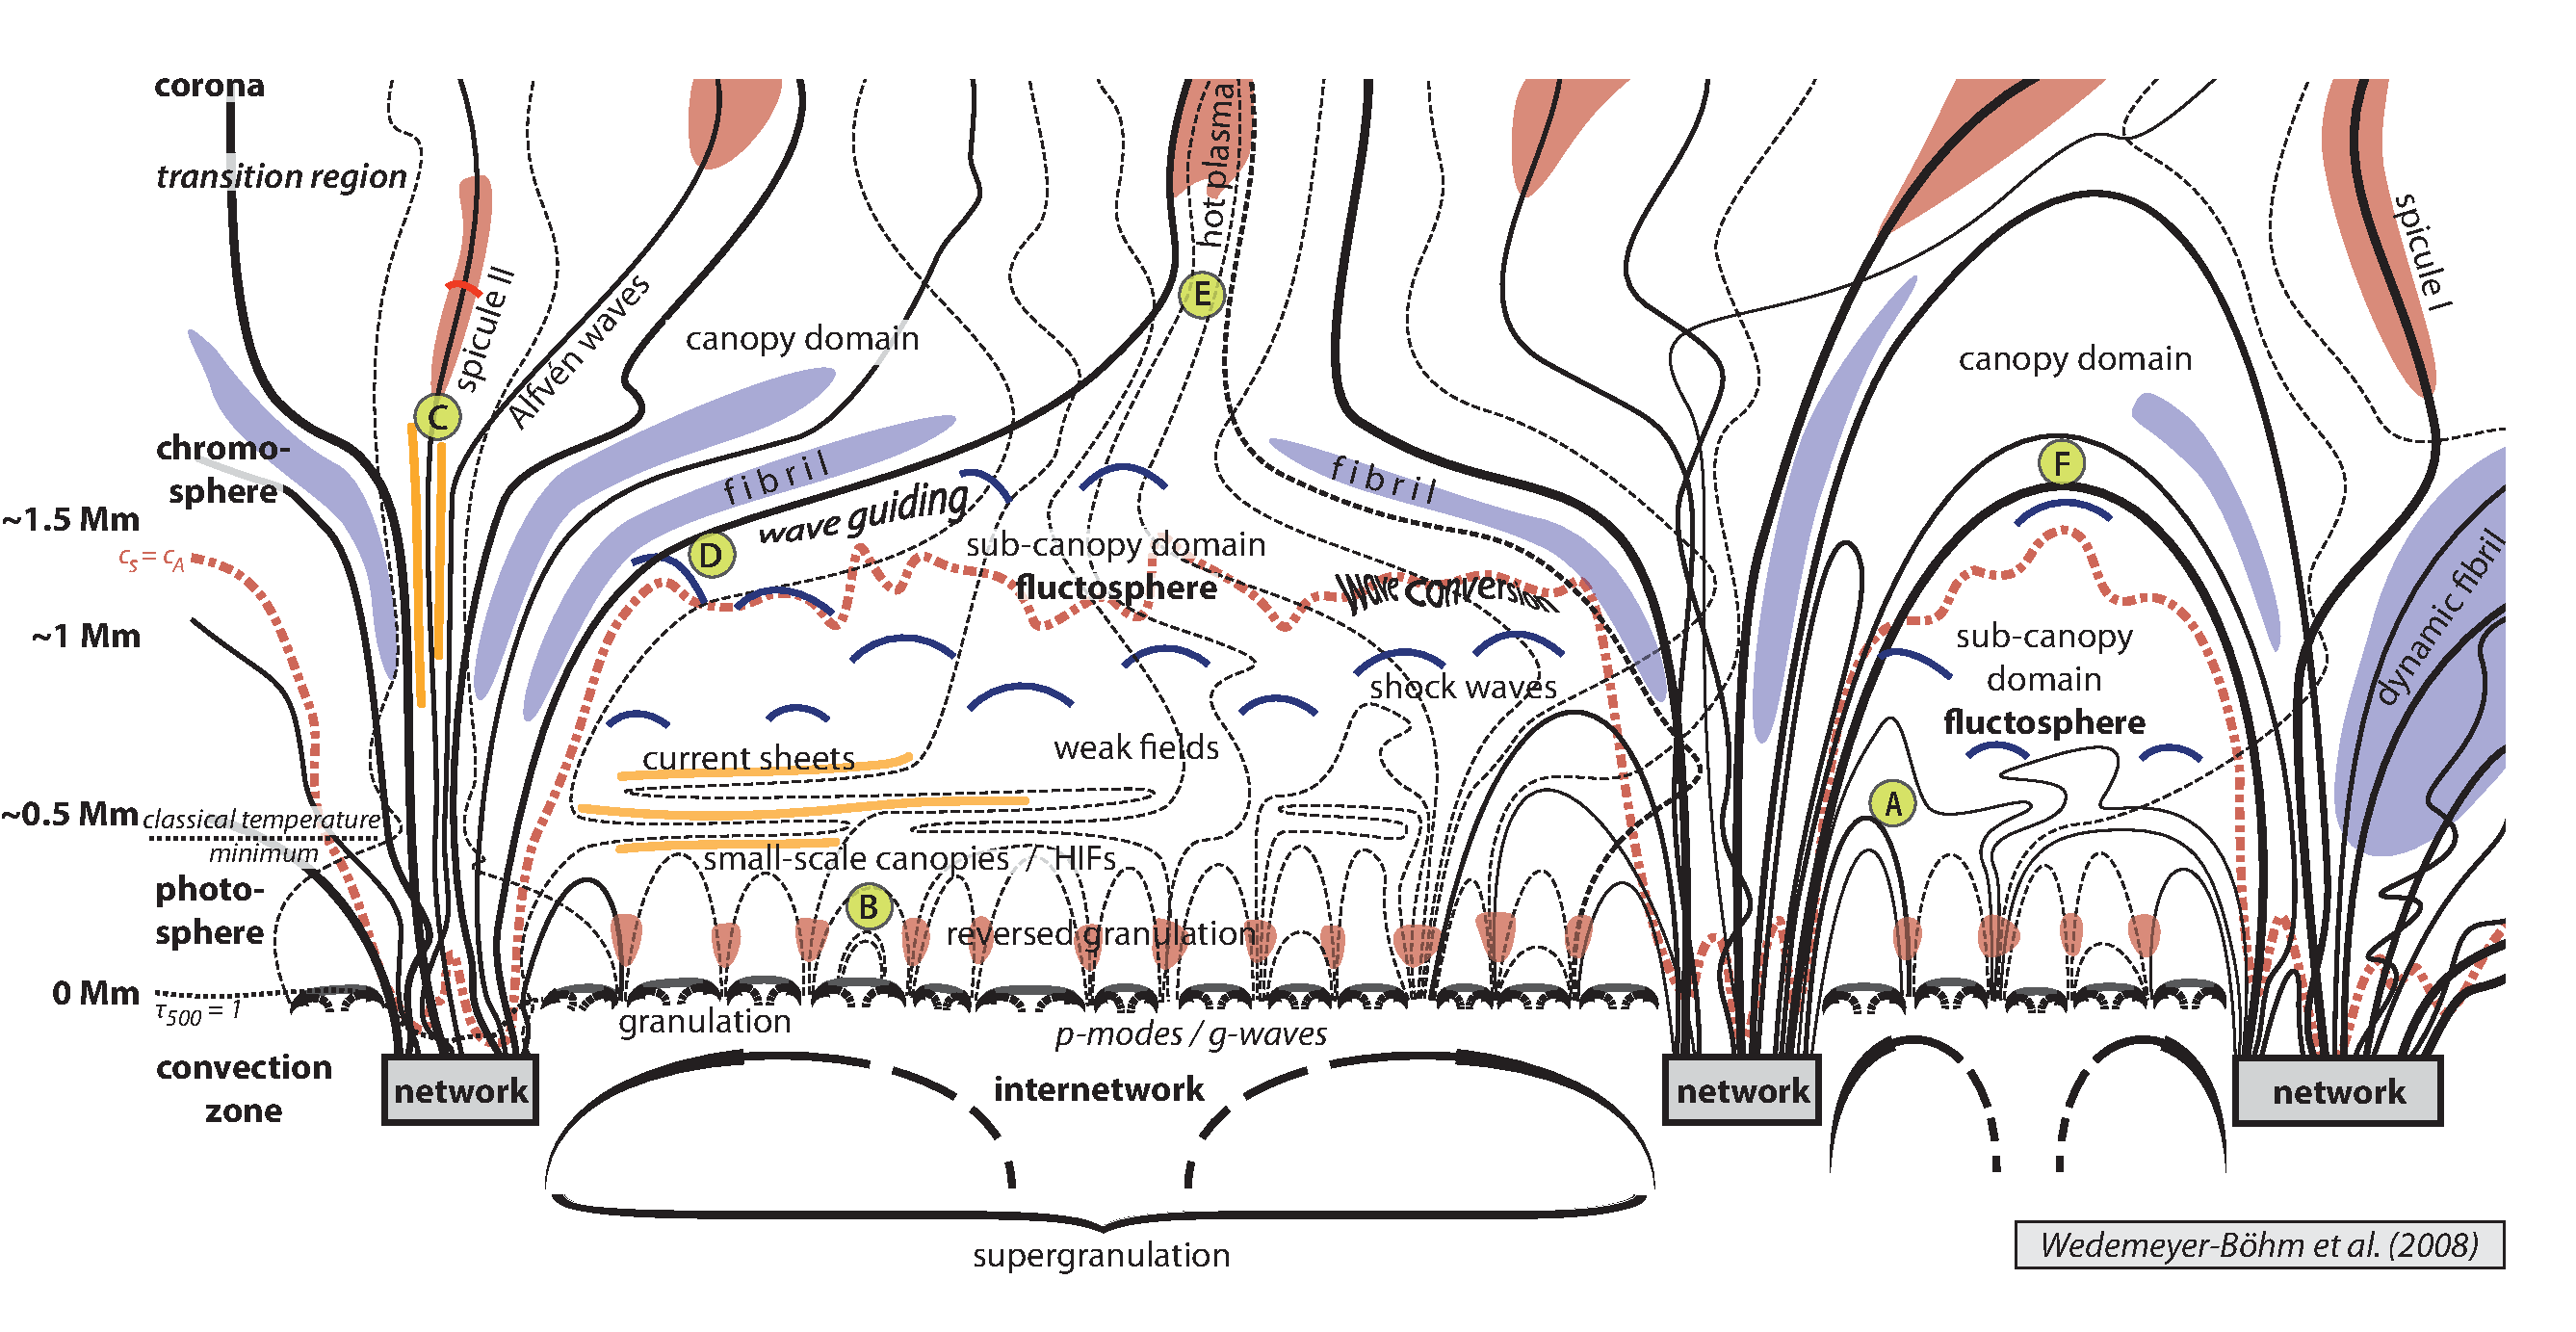
\includegraphics[width=\textwidth]{internetwork_sketch.pdf}
    	\caption{
		    	Reproduced from \cite{Sven} and is available online from \url{http://folk.uio.no/svenwe/public/pub08issi_wln.html}.
		    	}
    	\label{fig:chromo_field}
    \end{sidewaysfigure}
            
    Figure \ref{fig:chromo_field}....
      
    Running Penumbral Waves (RPWs), are a phenomenon discovered by \cite{Zirin1972} and \cite{Giovanelli1972}. 
    Observed in H$\alpha$ in sunspot penumbrae, they are seen as a wave train of enhanced darkness that moves from the umbra to the penumbra.
    They tend to be concentric and cover a large azimuthal angle.
    On average, they have a speed of $15$ to $20$ km s$^{-1}$ before slowing to $5$ to $7$ km s$^{-1}$ at the end of the penumbra.
    They have a typical period of $200$ to $300$ seconds. 
    Common interpretation is that much like the $3$-minute oscillations, they are slow magneto-acoustic wave propagating upwards along the inclined magnetic field and the radial outwards movement is actually a visual pattern \citep{UTMO,ORWS,OASO}.
    This is expanded on in Chapter \ref{chapter5}.
    
    Finally, we discuss the existence of a Moreton wave \citep{1960AJ.....65U.494M}.
    These are seen in H$\alpha$ wings as a dark and then a bright front.
    They travel away from flaring regions and are generally confined to a specific arc.
    They are more of a pulse than a wave and can travel at speeds up to $2000$ km s$^{-1}$.
            
\subsection{The transition region}

    Above the chromosphere, is a thin ($\approx100$ km) layer where the temperature rises rapidly from 20,000 K to 1,000,000 K.
    This is called the transition region.
    The rate of the increase is exponential and the density in this region decreases at a similar rate.
    In the bottom image of Figure \ref{fig:photosphere}, which displays the temperature and density of a semi-empirical model of the quiet Sun, this behaviour can be seen.
    This clearly means that the region is very non-uniform and \cite{tian2009solar} suggest that the height varies depending on what magnetic features are below the transition region.
    It cannot be observed from the surface of Earth, but can be from space-borne instruments sensitive to ultraviolet (UV) and extreme ultraviolet (EUV) light.
    
    Spicules, as discussed above, rise to large heights and it had been hypothesized that the TR would be a boundary.
    The spicule should hit the TR and create some form of a disturbance.
    These were discovered and called Transition Region Quakes (TRQs), found using the Extreme-Ultraviolet Imaging Spectrometer (EIS) instrument on-board the Japanese satellite Hinode.
    Coupled with MHD simulations, the disturbance was identified as a fast magneto-acoustic-gravity wave \citep{0004-637X-743-1-14}.
    These events further cement the link between the lower solar atmosphere and the higher regions.
    
\subsection{The corona}
\label{corona}

    The next layer is the outer atmosphere of the Sun is called the corona.
    It is most easily seen during a total solar eclipse, but also observable using a coronagraph \citep{markus2004physics}.
    The sheer scale of the corona is impressive.
    It extends many solar radii away from the solar surface and it is continuously expanding into the solar system which known as the solar wind.
    This entire region is called the heliosphere and this extends far past the orbit of Pluto.
    
    The average temperature of the corona is about 1-2 MK, however, it can reach temperatures as high as 8-10 MK \citep{markus2004physics}.
	The physical processes that account for the high temperature of the corona is still unknown, but two main hypotheses are in contention.
    The first one is called magnetic reconnection. 
    This process is where magnetic field changes its topology and the magnetic energy stored within the field is converted to kinetic and thermal energy and thus the plasma that is present in these reconnection regions will be heated. 
    The second one is MHD waves.
    The Sun creates a large amount of energy and the idea is that MHD waves can channel this energy from the convection zone through the various layers of the solar atmosphere and then into the solar corona.
	It requires that theses MHD waves are able to dissipate their energy into the plasma in order to heat this plasma.
    
    In all likelihood, a combination of these two main ideas will be the source behind coronal heating.
    This topic has been heavily researched for many decades and you can see reviews by \cite{erdelyi2004heating} and \cite{Parnell2012}.
    The most recent development has shifted the question, from ``how do you heat the corona?'' to ``how do you heat the chromosphere?'' \citep{Aschwanden2007}.
    
    The corona is host to many structures: X-ray bright points, plumes, prominences, streamers, coronal loops and coronal holes.
    When using a wavelength filter that samples higher temperature plasma ($\ge1$ MK), loop structures can be seen that rise several mega-meters in height.
    These are called coronal loops and they display a wide range of oscillations.
    See \cite{2010LRSP....7....5R} for a detailed review of coronal loops.
    Seismology of these loops has estimated the background quantities such as density and magnetic field strength of these loops (see \cite{2005RSPTA.363.2743D} or \cite{Banerjee2007} for a detailed review). 
    ARs  will also be the areas where flares or coronal mass ejections will originate from, since they contain large amounts of stored magnetic energy.
    
    These are the most spectacular events produced by the Sun.
    The amount of mass and energetic particles ejected can be considered scary, as these events have a direct impact on the Earth if the ejected material reaches Earth, from simply creating the aurora near the poles or in certain situations the disruption of radio transmissions, damage to satellites and electrical transmission lines.
    So it is important to understand the formation mechanism of these events so we can predict them and take measures to limit their damage.
    This is the realm of space weather research. 
    
    For a long time, it was hypothesised that MHD waves could not propagate into the corona due to the acoustic cut-off frequency.
    The launch of the Transition Region And Coronal Explorer (TRACE) space solar telescope changed this \citep{TRACE,TRACE1}.
    Numerous MHD oscillations where observed: damped transversal oscillations \citep{8007,2002A&A...394L..39G}, standing fast kink waves \citep{1999ApJ520880A,1999Sci...285..862N,1999SoPh..187..261S}, standing acoustic modes \citep{2003A&A...406.1105W}, fast sausage \citep{2001MNRAS.326..428W,2002MNRAS.336..747W,2003A&A...406..709K}, fast kink waves \citep{2005A&A...430L..65V}, propagating acoustic modes \citep{1997ApJ...491L.111O,2000A&A...355L..23D,2002A&A...393..649M} and torsional modes \citep{1998A&A...337..287E}. 
    This led to a large focus on coronal seismology which allows the estimation of the background properties of coronal loops using the observed properties of these waves.
    See a review on this topic by \cite{lrsp-2005-3} or \cite{MHDOS}.
    Finally, EIT waves were discovered using the Extreme Ultraviolet Imaging Telescope (EIT) instrument onboard the Solar and Heliospheric Observatory (SOHO) space satellite \citep{1998GeoRL..25.2465T}.
    These are large single-pulsed propagating fronts which appear to move unhindered throughout the corona after a large-scale event (such as a flare).
    They are believed to be associated with Moreton waves.
        
    Overall, this has been a brief overview of the history of the Sun, its interior and atmosphere. 
    For a more detailed introduction to the Sun, see \cite{priest1984solar} or \cite{2014masu.book.....P} and see \cite{markus2004physics} for a detailed overview of the solar corona.
    
\section{Magnetohydrodynamics}

    The mathematical underpinning used in solar physics is called magnetohydrodynamics (MHD).
    It adds the effects of a magnetic field to the governing equations of fluid mechanics. 
    More accurately, it is the melding of Maxwell's equations to the Navier-Stokes equations.
    This is credited to Hannes Alfv\'en, who won a Nobel Prize in Physics for this major contribution to science \citep{1942Natur.150..405A,erdelyi2007}.

\subsection{MHD equations}

    There are several equations that form the core of MHD and are solved in many different magnetic configurations. 
    The ultimate aim is to understand how these configurations will evolve in time or how they react to external factors.
    Further, they are solved to find out what kind of waves these configurations can support and how these waves perturb the system. 
    The MHD equations include many physical effects, however, we have taken the ideal assumption; adiabatic, inviscid, non-radiative, no thermal conduction and no resistivity.
    This is ideal MHD and the resulting equations are,
    \begin{align}                                                         
        \dfrac{\partial \rho }{\partial t} + \nabla \cdot (\rho \boldsymbol{{v}}) =       
        0,\tag{Mass Conservation}\\                                  
        \rho \dfrac{{D}\boldsymbol{{v}}}{{D}t} =
        -\nabla p + \dfrac{1}{\mu}(\nabla \times \boldsymbol{{B}}) \times \boldsymbol{{B}} + \rho \boldsymbol{{g}},\tag{Equation of Motion}\\
        \dfrac{{D}}{{D}t} \left(\dfrac{p}{\rho^\gamma} \right)  = 0,\tag{Energy Equation}\\       
        \dfrac{\partial \boldsymbol{{B}}}{\partial t} = \nabla \times (\boldsymbol{{v}} \times \boldsymbol{{B}}),\tag{Induction Equation}               
    \end{align}
    subject to
    \begin{align}
        \nabla \cdot \boldsymbol{{B}} = 0,\tag{Solenoid Equation}\\
        p = {k_B} \dfrac{\rho}{{m}} {T},\tag{Ideal Gas Law}\\  
        \boldsymbol{{E}} = - \boldsymbol{{v}} \times \boldsymbol{{B}},\tag{Ohm's Law}\\
        \boldsymbol{{j}} = \nabla \times \boldsymbol{{B}}/ \mu.\tag{Electric Current}                          
    \end{align}
    Here $\rho$ is the density, $\boldsymbol{{v}}$ is the velocity, $\frac{{D}}{{D}t}$ is the convective derivative $\left(\frac{\partial}{\partial t} + (\boldsymbol{{v}}\cdot\nabla)\right)$, $p$ is the pressure, $\gamma$ is the ratio of specific heats ($5/3$ for an ideal mono-atomic gas), $\boldsymbol{{B}}$ is the magnetic field, ${k_B}$ is Boltzmann's constant, ${m}$ is the mass, ${T}$ is the temperature, $\boldsymbol{{E}}$ is the electric field, $\boldsymbol{{j}}$ is the current density and $\mu$ is the vacuum permeability. 

    There are actually eight partial differential equations for eight variables.
    Both $\boldsymbol{{v}}$ and $\boldsymbol{{B}}$ have three components each and we have the density and temperature.
    From this, the typical recourse is to examine the case of small perturbations for the MHD quantities, i.e.,
    \begin{align*}                                                         
        \boldsymbol{{B}} &= \boldsymbol{{B}}_0 + \boldsymbol{{B}}_1(\boldsymbol{r},t)\\               
        \boldsymbol{{v}} &= \boldsymbol{0} + \boldsymbol{{v}}_1(\boldsymbol{r},t)\\               
        p &= p_0 + {p_1}(\boldsymbol{r},t)\\               
        \rho &= \rho_0 + {\rho_1}(\boldsymbol{r},t).\\              
    \end{align*}
    Here, subscripts are used to separate out the background (${B}_0$) and perturbation (${B}_1$) quantities.
    There is assumed to be no background flow and that all perturbations are much smaller than the background value (e.g., ${B}_0 \gg {B}_1$).      
    This leads to the linearised ideal MHD equations,
    \begin{align}                                                         
    \dfrac{\partial \rho_1 }{\partial t} + (\boldsymbol{{v}}_1 \cdot \nabla)\rho_0 + \rho_0 (\nabla \cdot \boldsymbol{{v}}_1) =       
    0,\tag{Mass Conservation}\\                                  
    \rho_0 \dfrac{\partial \boldsymbol{{v}}_1}{\partial t} =
    -\nabla p_1 + \dfrac{1}{\mu}(\nabla \times \boldsymbol{{B}}_1) \times \boldsymbol{{B}}_0 + \rho_1 \boldsymbol{{g}},\tag{Equation of Motion}\\
    \dfrac{\partial p_1}{\partial t} + (\boldsymbol{{v}}_1 \cdot \nabla)p_0 - c_s^2 \left( \dfrac{\partial \rho_1}{\partial t} + (\boldsymbol{{v}}_1 \cdot \nabla)\rho_0 \right) = 0,\tag{Energy Equation}\\       
    \dfrac{\partial \boldsymbol{{B}}_1}{\partial t} = \nabla \times (\boldsymbol{{v}}_1 \times \boldsymbol{{B}}_0),\tag{Induction Equation}\\
    \nabla \cdot \boldsymbol{{B}}_1 = 0, \tag{Solenoid Equation}               
    \end{align}
    where we can define the first characteristic speed in MHD, the sound speed, $c_s^2 = {\gamma p_0}/{\rho_0}$.
    There is another important characteristic speed and that is the Alfv\'{e}n speed, $c_A^2 = {{B}_0^2}/{\sqrt{\rho_0}}$.
    These equations need to then be applied to an equilibrium and, since the focus is sunspots and pores, a cylindrical flux tube is the ideal choice.
    
\subsection{MHD waves in cylindrical flux tubes}

    To understand the observed oscillations in sunspots and pores, it is important to investigate the nature of oscillations within an idealised model of these structures.
    However, before this occurs, a quick comment on MHD waves in a uniform infinite plasma atmosphere.
    Table \ref{tab:uniform_medium} summarises how MHD wave mode behaves within the traditional model used to explain MHD to undergraduates.
    This model is a uniform unbounded (i.e., infinite) atmosphere with a background magnetic field that is purely vertical.
    Three wave modes are present in this model, the Alfv\'{e}n mode, the fast mode and the slow mode.
    To summarise, the Alfv\'{e}n perturbs the velocity in a perpendicular direction to its propagation direction. 
    It also only propagates along the magnetic field lines and not perpendicular.
    For the fast and slow wave mode, the velocity perturbation is not perpendicular to the angle of propagation.
    The important distinction between the fast and slow mode in this model is that the slow mode does not propagate perpendicular to the background magnetic field, while the fast mode is isotropic.
    The effect of plasma-$\beta$ in this regime is to simply change the speed at which the slow and fast mode will propagate at.  
    This results tend to be summarised in Friedrich diagrams. 
    In the context of a cylindrical tube, only the fast and slow modes are discussed.
             
    \begin{sidewaystable}
	    \centering
		\begin{tabular}{lccc}
   			&			& $\beta \gg 1$, $\va \ll \vs$	&   $\beta \ll 1$, $\va \gg \vs$ 	 	\\
   			\vspace{-3mm} \\
   			\hline
   			\hline
   			\vspace{-2mm} \\
   			& $\bm{{k}} || \Beq$		& Alfv\'{e}n wave, $\vph^2 \sim \va^2$		& Alfv\'{e}n wave, $\vph^2 \sim \va^2$	\\
   			$\bm{{k}} \cdot \boldsymbol{{v}}_1 = 0$	&					&									&								\\
   			& $\bm{{k}} \perp \Beq$	& Alfv\'{e}n wave -- does not propagate 		& Alfv\'{e}n wave -- does not propagate	\\
   			\vspace{2mm} \\
   			& 					& Fast wave, $\vph^2 \sim \vs^2$	 		& Fast wave, $\vph^2 \sim \va^2$		\\
   			& 					& approximately isotropic	 			& approximately isotropic		\\
   			& $\bm{{k}} || \Beq$		& magnetic and kinetic pressure in phase	& magnetic and kinetic pressure in phase	\\
   			& 					& Slow wave, $\vph^2 \sim \va^2$	 		& Slow wave, $\vph^2 \sim \vs^2$		\\
   			& 					& magnetic and kinetic pressure out of phase	& magnetic and kinetic pressure out of phase	\\
   			$\bm{{k}} \cdot \boldsymbol{{v}}_1 \neq 0$&					&									&							\\
   			& 					& Fast wave, $\vph^2 \sim \vs^2$	 		& Fast wave, $\vph^2 \sim \va^2$		\\
   			& $\bm{{k}} \perp \Beq$	& approximately isotropic	 			& approximately isotropic		\\
   			& 					& magnetic and kinetic pressure in phase	& magnetic and kinetic pressure in phase	\\
   			& 					& Slow wave -- does not propagate	 		& Slow wave -- does not propagate		\\
   			\hline
   			~&~&~ \\
   		\end{tabular}
		\caption{
				 Phase speeds of the slow, fast and Alfv\'{e}n waves for a uniform unbounded magnetised plasma.
			     Adapted from \cite{jess2015multiwavelength}.
			    }
		\label{tab:uniform_medium}
     \end{sidewaystable}
     
    The most iconic investigation into this was undertaken by Edwin and Roberts in 1983 \citep{WPMC}.
    Their analysis is based on the non-slender flux tube, where the tube radius is greater or equal to the wavelength of the oscillations.
    Further it ignores the effects of gravity (i.e., the stratification of the atmosphere), which is important when the wavelength is comparable to the atmospheric scale height and in the photosphere this is the case \citep{LNLMHD}. 
    It is important to note that in thin flux tubes, there are two other characteristic wave speeds.
    One is a subsonic, sub-Alfv\'{e}nic speed, $c_T$ (defined later on), and the other is the ``mean'' Alfv\'{e}n speed, $c_k$.

    The model is as follows, a cylindrical magnetic flux tube of radius $a$ with its own density ($\rho_0$), pressure ($p_0$) and magnetic field (${B}_0\textbf{\^{z}}$) is embedded in a magnetic environment with a similar profile (${B}_e \textbf{\^{z}}$, $\rho_e$ and $p_e$).   
    The density and pressure are uniform throughout the medium.
    The top image of Figure \ref{fig:fluxtube} is a schematic drawing of this model. 
        
    \begin{figure}
        \centering
        \begin{subfigure}[b]{0.75\textwidth}
            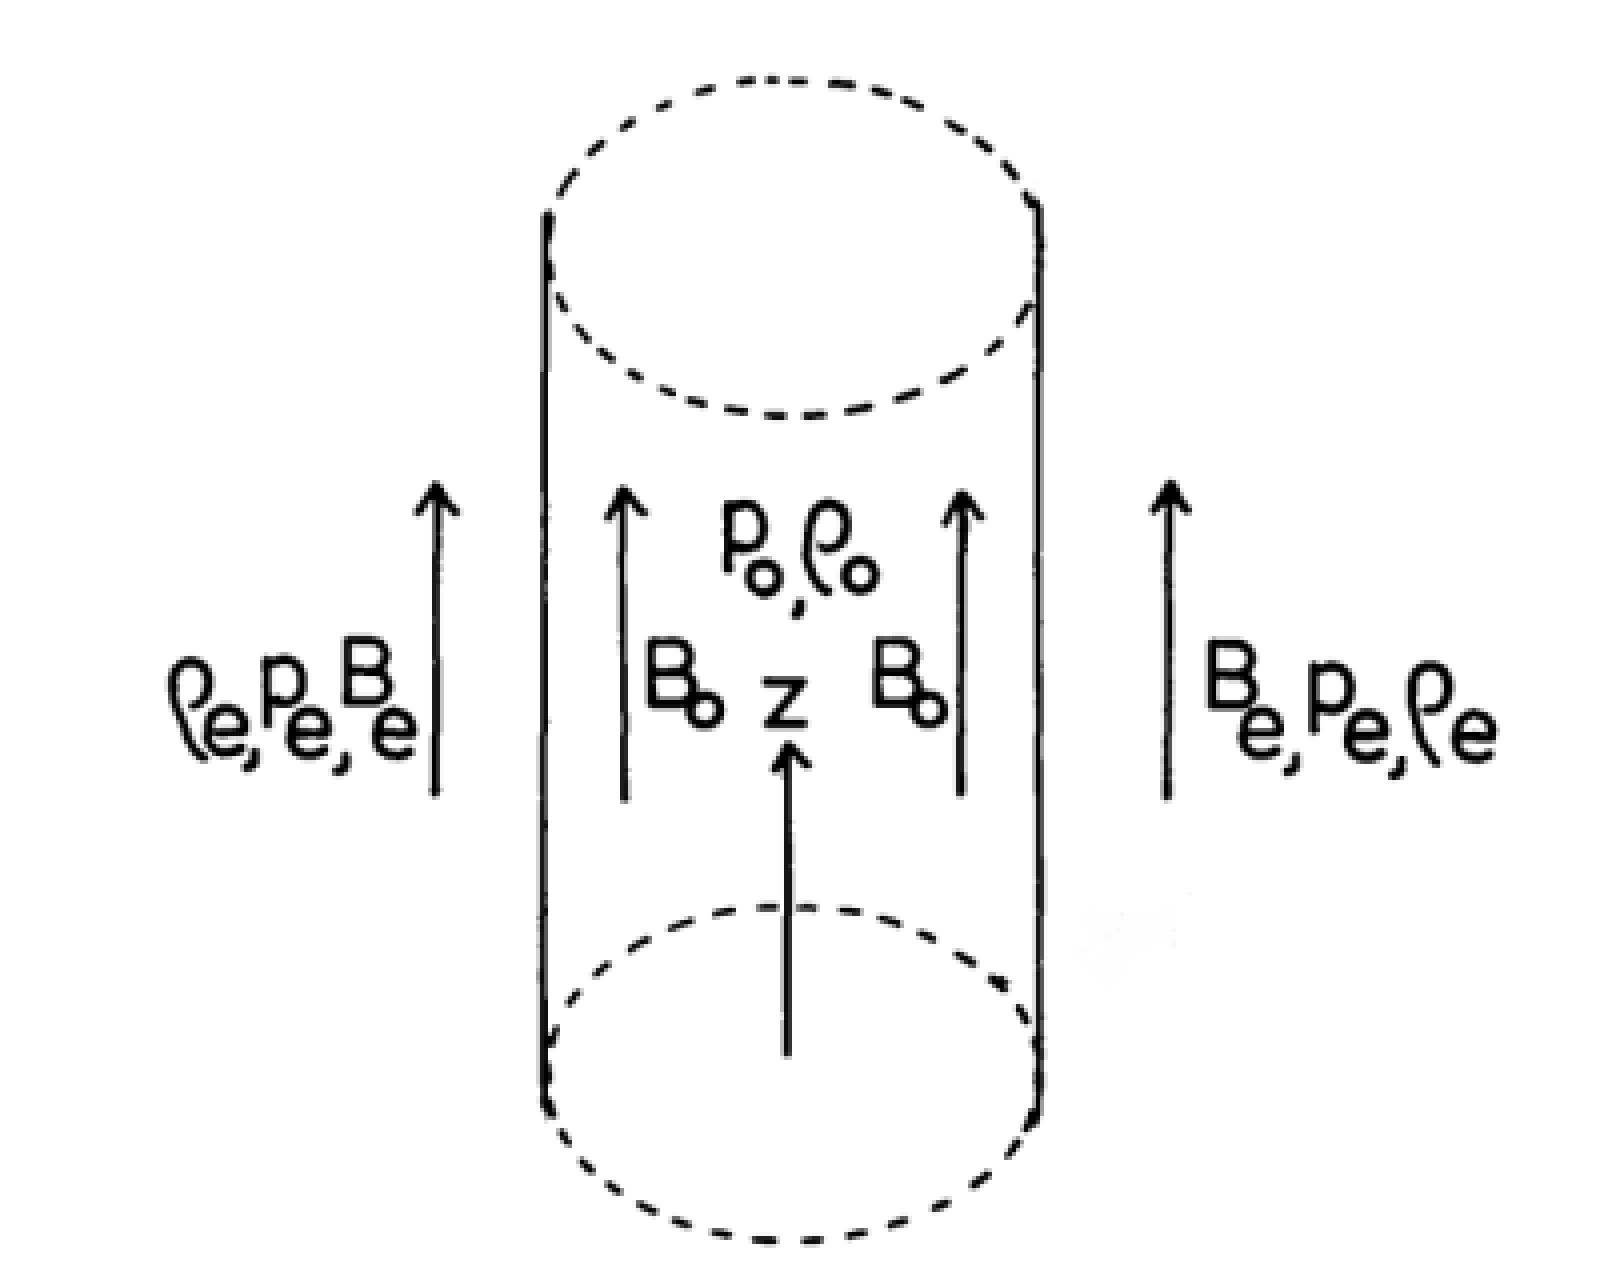
\includegraphics[width=\textwidth]{Fluxtube}
        \end{subfigure}\\~\\
        \begin{subfigure}[b]{0.65\textwidth}
            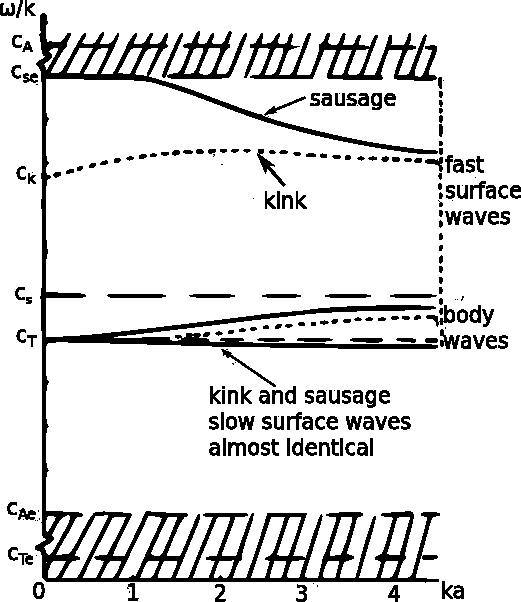
\includegraphics[width=\textwidth]{dispersion}
        \end{subfigure}
        \caption{
                \textit{(top)} The equilibrium conditions used to model wave behaviour in a magnetic flux tube.
                Image is a modified version of Figure 1 from \cite{WPMC}.
                \textit{(bottom)} The dispersion relationship derived from the MHD equations under photospheric conditions ($c_A > c_{se} > c_k > c_{Ae} $).
                The hatched areas are the excluded  values of $\omega$ and $ka$.
                Image is a modified version of Figure 2 from \cite{WPMC}.
                }
        \label{fig:fluxtube}
    \end{figure}
    
    This is the starting point for deriving the dispersion relation for MHD waves in a magnetic flux tube.
    It is assumed that this system is in equilibrium.
    Perturbations to the equilibrium conditions then add extra terms to the ideal MHD equations (the equations above).
    By introducing the Fourier decomposition of the perturbations, they show that the amplitude term is the Bessel equation.
    When bound on the axis of the cylinder ($r=0$), two solutions exist for either the body or surface wave.
    In the external atmosphere, the assumption of no propagation of energy away from or towards the cylinder allows the solution for the amplitude to be found for the external atmosphere.
    Further, the kinetic and magnetic energy density tend to zero as $r\rightarrow\infty$.
    Continuity at the boundary ($r=a$) has to be kept (radial velocity component $v_r$, and the total pressure) which yields the dispersion relations for surface waves and body waves \citep{WPMC}.
    These are,
    \begin{align}
        \rho_0 (k^2 c_A^2 - \omega)m_e \dfrac{K_n^\prime(m_e a)}{K_n(m_e a)} &= \rho_e (k^2 c_{Ae}^2 - \omega)m_0 \dfrac{I_n^\prime(m_0 a)}{I_n(m_0 a)} \tag{Surface, m$_0^2 > 0$} \\
        \rho_0 (k^2 c_A^2 - \omega)m_e \dfrac{K_n^\prime(m_e a)}{K_n(m_e a)} &= \rho_e (k^2 c_{Ae}^2 - \omega)n_0 \dfrac{I_n^\prime(n_0 a)}{I_n(n_0 a)} \tag{Body, m$_0^2 = -n_0 < 0$} 
    \end{align}
    where, $K_n$ and $I_n$ are Bessel functions of order n, $K_n^\prime$ and $I_n^\prime$ are the derivatives of the Bessel functions, $m_0$ and $m_e$ are the internal and external wavenumber, defined as, $$\dfrac{(k^2 c_{s}^2 - \omega^2)(k^2 c_{A}^2 - \omega^2)}{(c_{s}^2 + c_{A}^2)(k^2 c_{T}^2 - \omega^2)},$$ and $c_{T}$ is the tube speed, $$c_{T} = \dfrac{c_s^2 c_A^2}{c_s^2 + c_A^2}.$$
    Finally, these dispersion relations are solved under photospheric conditions (plasma-$\beta << 1$, such that, $c_A > c_{se} > c_k > c_{Ae} $) and the solutions are plotted at the bottom of Figure \ref{fig:fluxtube}.
        
    These dispersion relations are important as they detail the way in which waves propagate through numerous flux tube sizes.
    It shows the limits of the wave solutions indicating in what regimes they cannot exist.
    Surface waves are dispersive as their phase speed depends on the wavenumber.
    There are slow body waves which are both sausage, kink and fluting modes and these modes have a phase speed between the tube and sound speeds.
    Slow surface waves have phase speeds close to the tube speed. 
    There is also a surface wave with a phase speed close to the kink speed and another surface wave near the sound speed.
    If one can measure the phase speed of an observed wave and the $ka$ of the flux tube, one can also likely identify the observed waves.
    This has been attempted by \cite{2015A&A...579A..73M}.
    
    One factor that has been neglected is the mode number ($n$), its value governs the way in which the wave perturbs the flux tube.
    This gives us the name: sausage ($n=0$), kink ($n=1$) and fluting ($n>1$).
    These different wave modes cause characteristic physical effects which can be used to identify each different wave mode.
    
    Figure \ref{fig:tube} shows the physical changes to the flux tube, caused by each different wave mode.
    Below, when a quantity is talked about, the focus is on the perturbation of that quantity.
    The first diagram (labelled a), shows how the slow wave affects the flux tube. 
    The velocity is primarily longitudinal.
    Further, when the flux tube contracts the density decreases in that region indicating a phase difference of $\pi$, but this is also the same phase difference for the cross-sectional area and total intensity.
    The second diagram (labelled b), shows the fast sausage mode.
    The velocity is primarily radial and when the flux tube contracts the density in that region increases unlike the slow sausage mode.
    This means that the cross-sectional area and total intensity are in phase, as well as the magnetic field.
    These diagrams have been improved over time and movies have been created which can be found within several papers \citep{Morton2012,jess2015multiwavelength} and online sources (\url{http://www2.warwick.ac.uk/fac/sci/physics/research/cfsa/research/wpc/vis/} or \url{http://swat.group.shef.ac.uk/fluxtube.html}).
    Finally, the last diagram (labelled c) shows the kink wave mode.
    It is non-compressible (to the first order linear limit, long wavelength approximation) and perturbs the flux tube axis.
    This makes it very difficult to identify unless it is possible to isolate the central axis of the flux tube.
    This is quite difficult for a sunspot or pore, but it has been done for spicules and fibrils and  kink and Alfv\'en waves have been observed (see section \ref{chromo} for more details).
    
    \begin{figure}
    	\centering
    	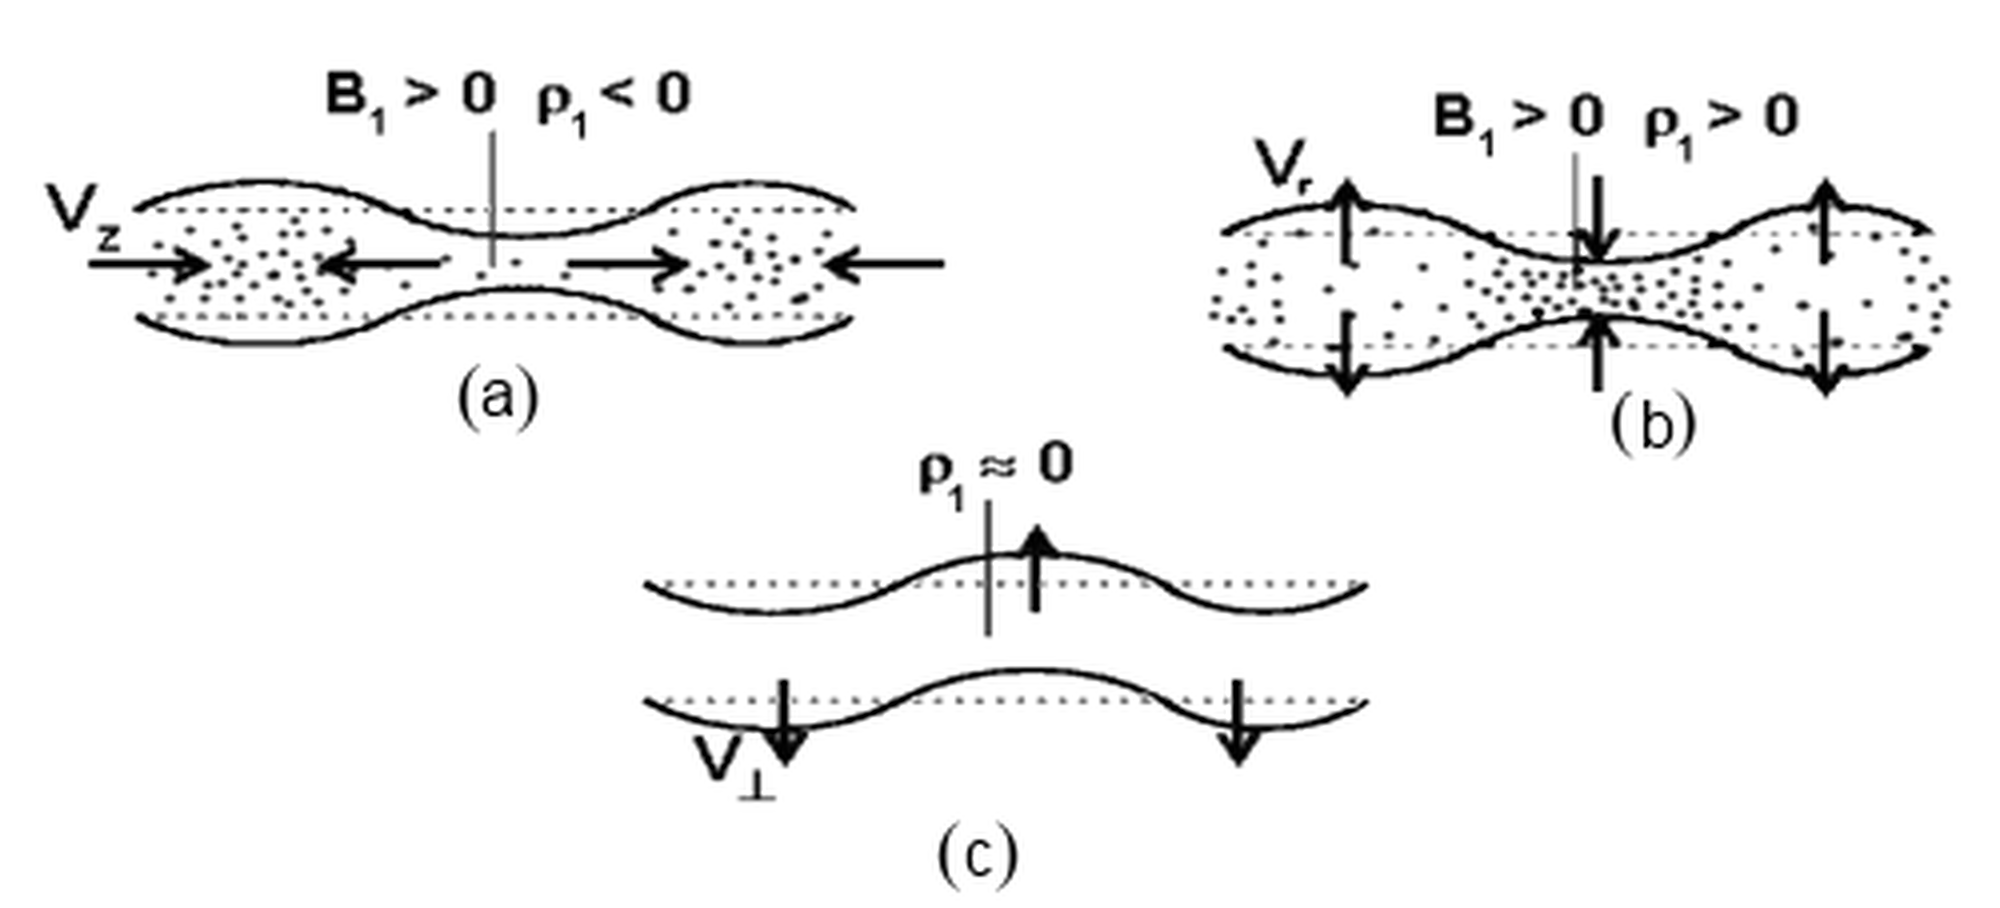
\includegraphics[width=\textwidth]{tube}
    	\caption{
    		The physical effects that each type of wave has on the flux tube.
    		(a) The slow magneto-acoustic waves (slow sausage mode) which cause anti-phase behaviour between the intensity and the magnetic field.
    		(b) The fast magneto-acoustic waves (fast sausage mode) which cause in phase behaviour between the intensity and the magnetic field.
    		(c) The fast magneto-acoustic waves (fast kink mode) which cause no magnetic field perturbations but cause $\pi/2$ phase behaviour between the intensity and velocity perturbation.
    		Image is a modified version of Figure 1 from \cite{CLOO}.
    	}
    	\label{fig:tube}
    \end{figure}
   
	While these are toy arguments and descriptions, these phase relations have been derived by several authors \citep{PMHDW,Moreels2013,Moreels2013b,2015A&A...579A..73M}.
    They have taken complex models of embedded flux tubes to derive an almost full set of phase relations for many of the MHD wave modes and whether they are standing or propagating.
	The main conclusions from \cite{Moreels2013} and \cite{Moreels2013b} is that fast and slow sausage modes have a different phase behaviour; namely that slow modes have an in phase behaviour (i.e., $0$ degrees phase difference between the cross-sectional area and the Lagrangian intensity oscillations), while fast modes have an anti-phase behaviour (i.e., $180$ degrees phase difference between the cross-sectional area and the Lagrangian intensity oscillations).
    Throughout all of this thesis we use the Lagrangian intensity variations, i.e., the intensity variations when following the motion of the plasma, when discussing the intensity. 
     
    Table \ref{tab:phase} summarises the phase relations between the intensity, Doppler velocity, magnetic field and for the cross-sectional area and intensity for each wave type and whether it is a standing or propagating wave.
    This table contains the information that will be used later on in this thesis, in order to identify the observed oscillations which occur within the numerous magnetic structures analysed. 
    Since the focus has been on compressive perturbations, kink waves are neglected from this point onwards, as are Alfv\'en waves.
    However, see these recent review of both of these waves with regards to theory and observations \citep{Mathioudakis2013,jess2015multiwavelength}.
    It is important to note that the focus has been exclusively on MHD sausage waves within this thesis.
  
    \begin{table}
        \centering
        \begin{tabular}{l|c|c|c|c}
            &$\phi_{{B}}-\phi_{{v}}$&$\phi_{{v}}-\phi_{{I}}$&$\phi_{{I}}-\phi_{{B}}$&$\phi_{{S}}-\phi_{{I}}$ \\ \hline\hline
        Slow sausage propagating        & $\pi$ & 0 & $\pi$ & 0 \\
        Slow sausage standing           & $\pm\pi/2$ & $\pm\pi/2$ & $\pi$ & 0 \\
        Fast sausage propagating$^6$    & [0,$\pi$] & [$-\pi/2$,0] & [$-\pi/2$,0] & $\pi$ \\
        Fast sausage standing$^6$       & $\pm\pi/2$ & $\pm\pi/2$ & [0,$\pi$] & $\pi$  \\
        Fast kink propagating       	& $\pm\pi/2^3$ & $N/A^4$ & $N/A^4$ & $N/A^4$ \\
        Fast kink standing          	& [$\pi/2^1,\pi^2$] & $N/A^4$ & $N/A^4$ & $N/A^4$ \\ \hline
        \end{tabular}
        \caption{
            Shows the phase differences between three observables: the intensity, Doppler velocity and the magnetic field for each type of MHD wave and whether the wave is standing (S) or propagating (P).
            1 - Wave propagating anti-parallel to the magnetic field.
            2 - Wave propagating parallel to the magnetic field. 
            3 - Depending on the distance to the reflection boundary.
            4 - Kink modes are incompressible and thus have zero intensity fluctuations.
            5 - Fast sausage mode has zero LOS velocity fluctuations.
            6 - Surface mode only.
            Collated from these authors, \cite{CLOO,PMHDW,Moreels2013,Moreels2013b,2015A&A...579A..73M}}
        \label{tab:phase}
    \end{table}
    
	The previously derived theory \citep{Moreels2013,Moreels2013b,2015A&A...579A..73M,jess2015multiwavelength} gives an insight into the observational signatures that MHD sausage waves will exhibit within a magnetic waveguide.
	While the base signature will be the change of the cross-sectional area with respect to time and that this signal should be either in phase or out of phase with the total intensity signal. 
	What is missing from this, is whether the two MHD sausage modes (slow and fast) have characteristics that will either it easy or difficult to observe.
    \cite{Moreels2013} suggest that the fast MHD sausage mode, in photospheric conditions, should be able to perturb the radius up to 20\%.
    For the slow MHD sausage mode, the type of wave becomes important.
    For waves within flux tubes, there are two wave types: body and surface.
	For the slow MHD sausage surface mode, the perturbation amplitude is very small, below the resolution of current telescopes.
	However, the slow MHD sausage body mode, should be able to perturb the radius up to 10\%.
	The reason for this difference between the slow and fast mode is that the dominant velocity perturbation is longitudinal for the slow mode while it is radial for the fast mode.
    \cite{jess2015multiwavelength} suggest that the fast MHD sausage mode has a larger cross-sectional area perturbation as well as stronger density perturbations compared to the MHD slow sausage mode.
    Overall, the current research suggests that the effect of MHD sausage modes is observable with the current generation of ground-based telescopes.
\graphicspath{{Chapter2/Figs/}}

\chapter{Data collection and analysis overview}
	
	\vspace*{\fill}\par
    \pagebreak
	 
\section{Introduction}

	The current state of solar observations has never been more ideal.
	There is currently constant space-based monitoring of the Sun but also a myriad of high-quality ground-based solar telescopes in existence.
    This is coupled with a few small space-based telescopes and sounding rocket experiments.
	Furthermore, within the next decade, the largest ground-based solar telescope will open called the Daniel K. Inouye Solar Telescope (DKIST, formerly the Advanced Technology Solar Telescope, ATST) and several highly-advanced satellites will be launched (two of which will move in to very close orbit to the Sun).
	This will be an important era for solar physics.
	
	Numerous sources of solar data were used in the analyses presented here.
	Two telescopes will be the primary focus of this chapter: the Swedish Solar Telescope (SST) and Solar Dynamics Observatory (SDO).
	While data from other ground-based telescopes are used, having spent 10 days at the SST it receives a larger focus.
	These two telescopes offer some of the highest quality data available to a solar physicist.
	
	Data that is taken directly from any telescope will need to be corrected for any artefacts and this process is called data reduction. 
	Data reduction requires the creation of specific files called darks, flats and pinhole images.
	Darks are the images when there is no incoming light and displays the background noise of the camera.
	Flats are the images when the incoming light is uniform and this displays the imaging artefacts that come from the optics.
	Pinhole are images used to align the cameras along the optical path of the telescope.
	These images are applied onto the original data to reduce any imaging artefacts that are present within the original data.
	The final step is to remove the effects of the Earth's atmosphere and these methods are detailed later on.
	It should be noted that all data used had been reduced to a science ready level.
	
	Once the data is reduced, the method of analysis will need to be considered and it will vary depending on the scientific aims.
	Here, the aim was to measure the cross-sectional area and total intensity through time of sunspots and pores.
    Once these two properties have been measured, deducing any periods within these signals and calculating the phase difference between them is required and numerous signal analysis methods exist that aim to do just that.
    Three methods are employed which are the fast Fourier transform (FFT), Wavelet Transform (WT) and Empirical Mode Decomposition (EMD).  

    In this chapter, the telescopes and instruments will be details then the signal analysis methods are covered and the chapter ends on a brief analysis into the method used to measure the cross-sectional area for two example magnetic flux tubes.
	
\section{Sources of solar data}

	The work detailed within this thesis uses data from five telescopes: Swedish Solar Telescope (SST), Solar Dynamics Observatory (SDO), Dunn Solar Telescope (DST), Dutch Open Telescope (DOT) and the Swedish Solar Telescope (SVST).
    They are outlined below.
    
\subsection{Swedish solar telescope}

	The Swedish Solar Telescope is a one metre vacuum solar telescope located at the Roque de los Muchachos Observatory on La Palma in the Canary Islands.
	The SST was the replacement for the Swedish Vacuum Solar Telescope which used to occupy the same site and will be talked about later in this chapter.
	The SST has a $1.1$ m lens, of which only $1$ m is usable, which is connected to a several storey vacuum tower. 
    The light collected travels down the vacuum tower into a corrector system and then to the optics bench. 
    The usage of a vacuum tower means that the collected light does not pass through any air.
    This reduces any distortion that comes from the air being heated by the beam of light  and improves the overall image quality. 
    The scale of the SST can be seen in Figure \ref{fig:SST}.
    It shows the building that houses the SST and the tower that contains the vacuum tower can be seen.    
	\begin{sidewaysfigure}
        \centering
        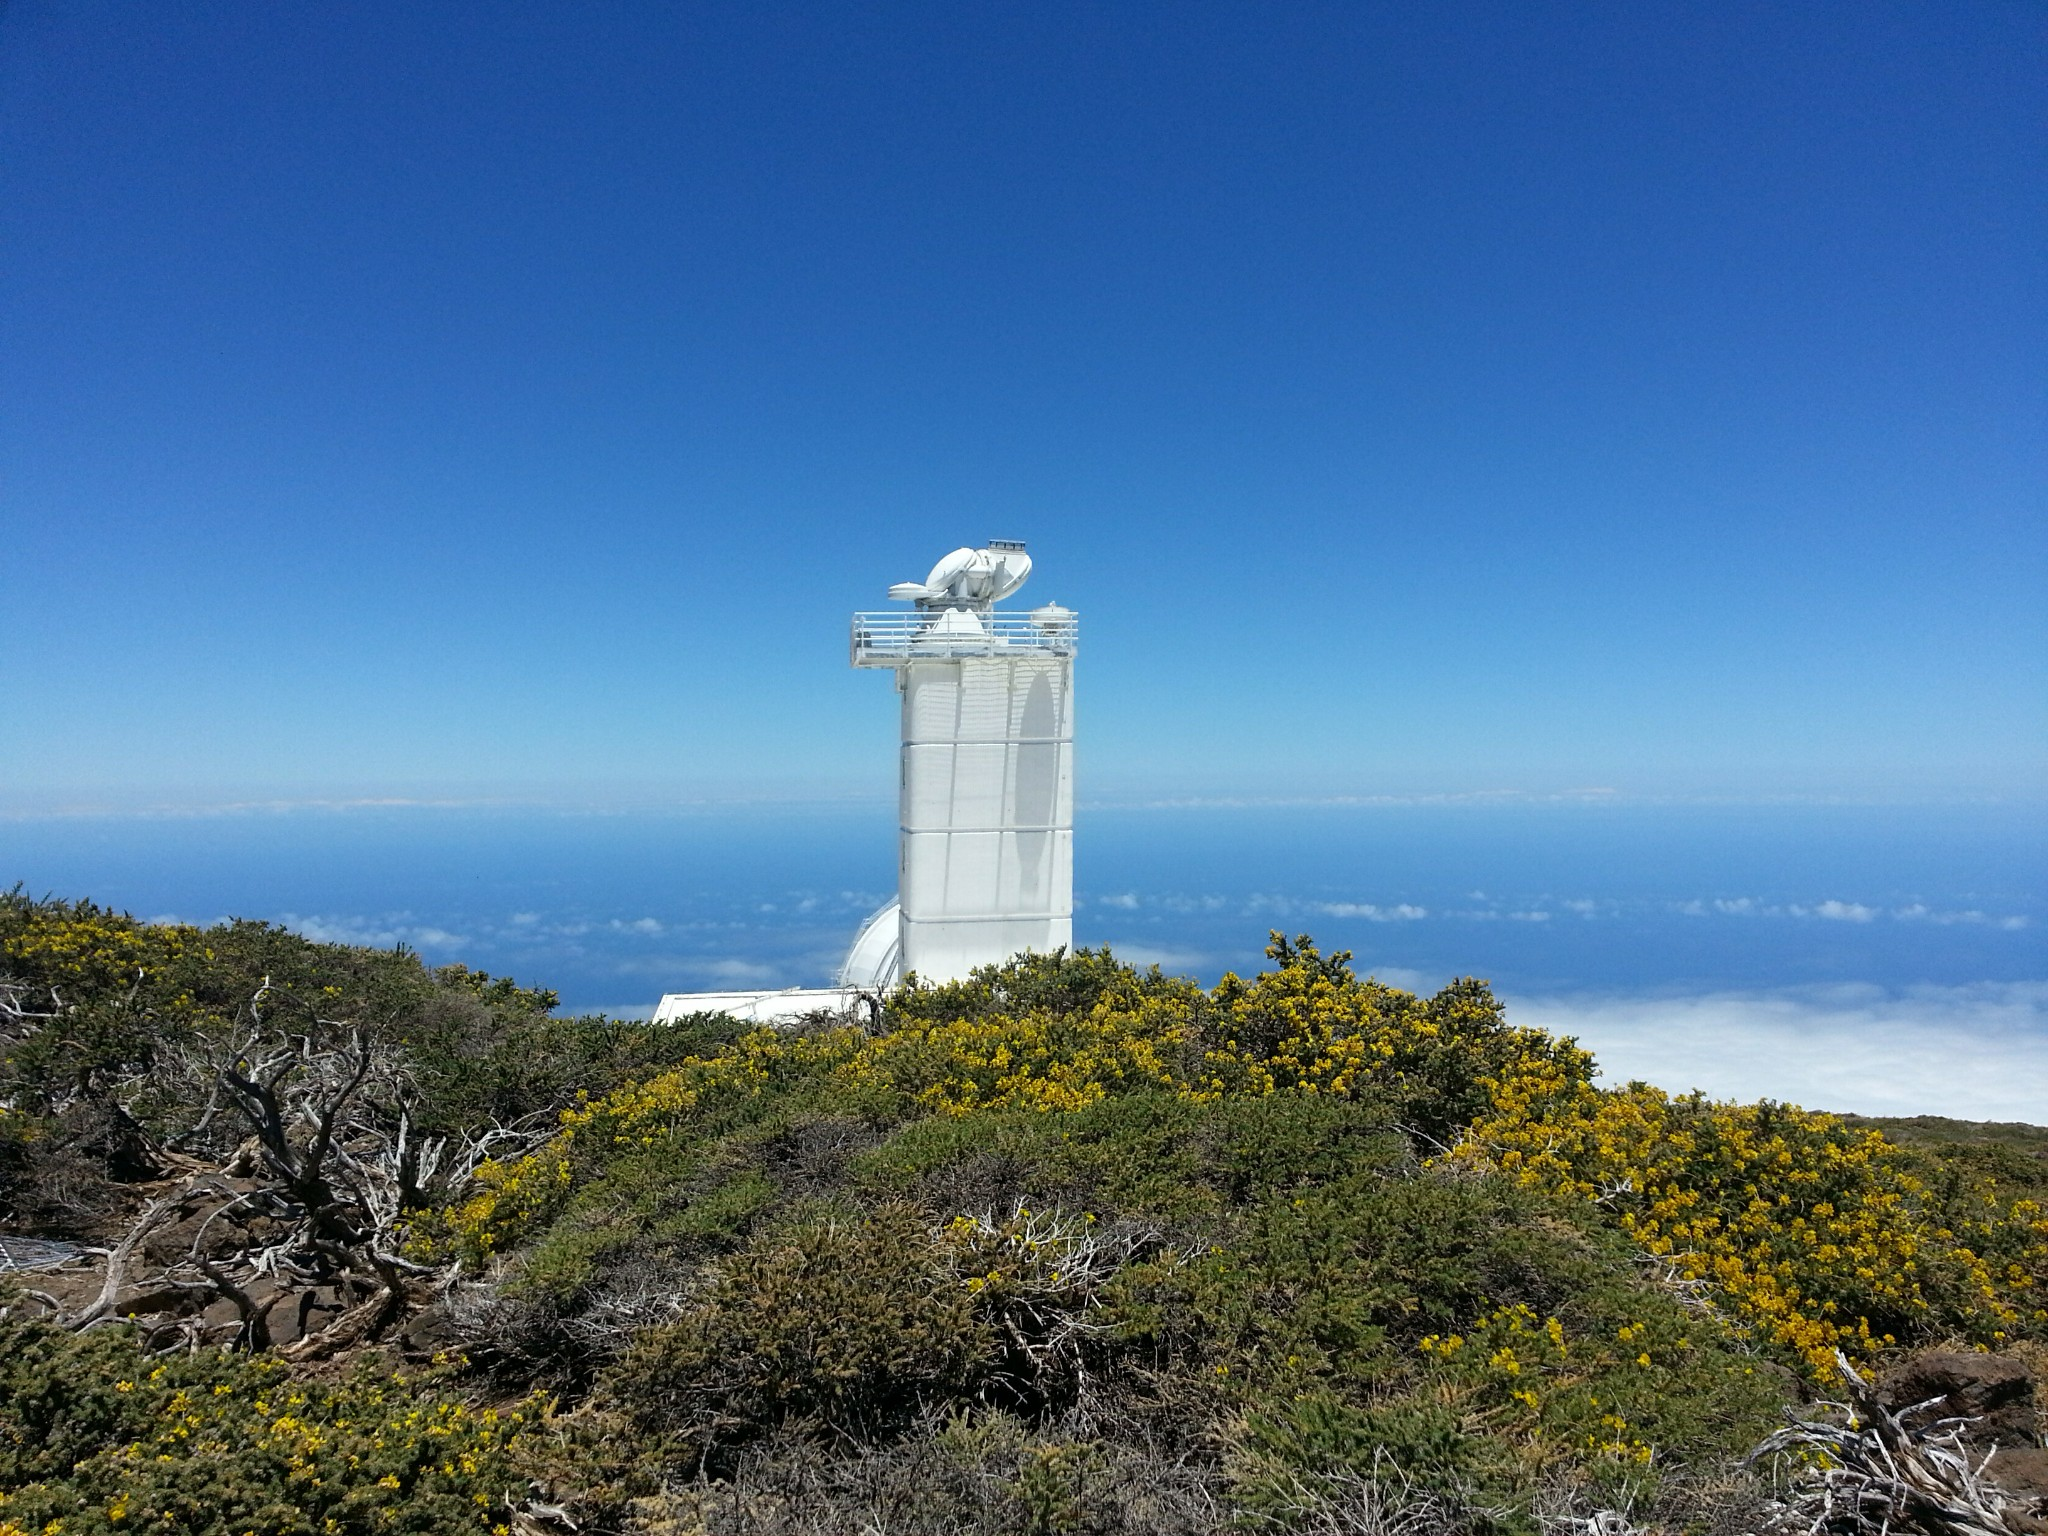
\includegraphics[width=0.75\textwidth]{SST.jpg}
        \caption{
            An image of the Swedish Solar Telescope taken from a ledge near the caldera on the island of La Palma that is part of the Canary Islands.
            The primary mirror housing can be seen at the top of the image, while the tower that conceals the vacuum tower can be seen beneath it.
            Copyright goes to the author.
           }
           \label{fig:SST}
   \end{sidewaysfigure}
         
    Further to this, the SST is equipped with an adaptive optics (AO) system. 
	AO is a term used for a process that will adjust the optics of the instrument in order to reduce the effects of turbulence from the Earth's atmosphere. 
	At a basic level, the AO at the SST has a sensor that monitors the wavefront of the incoming light wave and analyses how the wavefront is distorted.
	This distortion is counteracted by deforming a lens, made of a piezoelectric material, with a specific set of voltages to restore the wavefront.
	This is not the same method used by larger and newer optical telescopes used for astrophysics that have a deformable primary mirror in conjugation with a powerful laser.
	
	The SST has two instruments, the \textit{CRisp Imaging SpectroPolarimeter} (CRISP) and the \textit{TRI-Port Polarimetric Echelle-Littrow} (TRIPPEL).
	TRIPPEL is a spectrograph with a constant diffraction grating spacing but has a shape that is similar to a sawtooth-shaped step function.
    See \cite{2011A&A...535A..14K} for a full overview of this instrument.
    
	CRISP is a tunable dual Fabry-Perot filter system.
    The wavelength range is in the red wing (510-860 nm) and the light firstly goes through a selectable pre-filter dependent on the goals of the current observational sequence.
    This allows many wavelengths to be chosen with one instrument, which is required in order to observe the height variation of the solar atmosphere.
	The Fabry-Perot is made from a pair of partly reflective mirrors that are separated by a small distance.
    By varying the distance between the two mirrors, a specific wavelength can escape the mirror system and go to the cameras.
    With the ability to vary the distance between the mirrors, the Fabry-Perot system is able to investigate the line profile of many elements.
	Table \ref{crisp} has approximately a fourth of the wavelengths available with CRISP. 
	The selection of wavelengths here are the commonly used filters that appear in published papers.
	For example, the Fe I 630.26 nm line is used to observe the photosphere and clear granulation can be seen.
	More importantly, this wavelength is used to measure the photospheric magnetic field.
	    
	\begin{table}
         \begin{center}
         \begin{tabular}{|c|c|c|c|}
             \hline
             Pre-filter & Wavelength (nm) & FWHM (nm) & Line Core Height (km)\\
             \hline
             \ion{Mg}{} b & $517.33$ & .3 & $\le 1000$ \\
             \ion{Na}{D} & $589.7$ & .38 & $\le 500$ \\
             \ion{Fe}{I} & $630.26$ & .44 & $\le 250$ \\
             \ion{Ca}{II} k & $854.16$ & .93 & $\le 1300$ \\
             \ion{H}{$\alpha$} & $656.2$ & .49 & $\le 1500$ \\
             \hline
        \end{tabular}
        \caption{
                Summary of the more common wavelengths that are selectable with CRISP.
                Each filter has a name, wavelength at the line-core and the Full Width at Half Maximum (FWHM) and an average formation height of the line-core, which come from \cite{jess1}. 
                }
        \label{crisp}
        \end{center}
     \end{table}
	   
    An important wavelength is $656.3$nm and is commonly referred to as H$\alpha$.
    It is when an electron drops one energy level from the third shell to the second in a Hydrogen atom.
    This transition is the easiest method to observe the chromosphere and forms approximately $1.5$ Mm from the base of the photosphere.
    Understanding the chromosphere has become a topic of heavy interest as the ``Coronal Heating Problem'' shifted from the corona to the chromosphere over the past decade \citep{Aschwanden2007}. 
    Since the line core of H$\alpha$ samples the chromosphere, understanding how this line is formed within the solar atmosphere has become a very important topic. 
    
    However, H$\alpha$ line formation is a difficult topic.
    The line is highly complex, most likely it is dependant on numerous physical effects such as ionization or non-LTE effects. 
    Currently, the standard understanding of H$\alpha$ comes from radiative MHD simulations done, for example by \cite{Leenaarts2007} and \cite{Leenaarts2012}.
    From these two sources, a few properties and observations of the H$\alpha$ line core can be summarised.
    
    Current research suggests that structures that appear darker, such as fibrils, in the line-core are formed higher compared to other features.
    Further, the opacity of H$\alpha$ that is formed in the upper chromosphere is temperature insensitive.
    This means that the opacity of the line is mainly determined by the mass density at these regions.
    The results suggest that fibrils are mainly located within magnetically dominated (i.e., low plasma-$\beta$) regions between photospheric field concentrations of opposite polarity.
    These fibrils are aligned with the local magnetic field direction are located in regions where the local density is larger compared to the background chromosphere. 
    This effects the average formation height for H$\alpha$ by making it higher and thus the intensity is lower.
    Therefore, fibrils can be used to trace out regions of enhanced chromospheric mass density. 
    
    Finally, the light beam at the SST is spilt into two parts when CRISP is in use.
    The red wing goes to CRISP, while the blue part goes to a series of broadband cameras.
    These wavelengths are G-band and \ion{Ca}{K} which sample the photosphere.
    These offer some of the highest resolution images of the solar photosphere to date and are only used when the seeing is excellent. 
    Examples of the data from these cameras can be seen on the SST website (\url{http://www.solarphysics.kva.se/})
    
    To reduce SST data, the steps detailed at the start of this chapter will occur.
    However, the method used to remove the effects of the Earth's atmosphere from SST data is called Multi-Object Multi-Frame Blind Deconvolution (MOMFBD).
    This is a complex and computationally demanding method to improve the quality of the data without affecting the cadence of the observation data. 
    See \cite{Noort2005} for a full breakdown of this reduction method. 
    
\subsection{Solar dynamics observatory}

	Solar Dynamics Observatory is one of the latest space-based telescopes launched by National Aeronautics and Space Administration (NASA \citealt{2012SoPh..275....3P}).
	It can be considered as the replacement for the Solar and Heliospheric Observatory (SOHO \citealt{domingo1995soho}) and the Transition Region and Coronal Explorer (TRACE \citealt{TRACE}).
    Since 2010, it has been observing the Sun constantly beaming large quantities of data back to Earth.
	Without Earth's atmosphere in the way, it offers some of the clearest observations of the entire Sun to date. 
	The spacecraft houses three instruments: the \textit{Extreme Ultraviolet Variability Experiment} (EVE \citealt{2012SoPh..275..115W}), the \textit{Helioseismic and Magnetic Imager} (HMI \citealt{2012SoPh..275..229S}) and the \textit{Atmospheric Imaging Assembly} (AIA \citealt{2012SoPh..275...17L}).
	 
	HMI measures LOS velocities as well as the LOS and vector magnetic field of the photosphere.
	AIA is a multi-wavelength instrument and is able to take images of the solar surface to the outer reaches of the solar atmosphere.
    This has offered an unprecedented view of the many layers of the solar atmosphere at the same time.
    This view can be seen in Figure \ref{fig:SDO}, which shows the full temperature range of AIA as well as an HMI image.
    The figure showcases almost every wavelength that is available on AIA, from the low temperature lines such as $170$ nm that sample the photosphere, to the hotter lines that display the complex structure within the corona such as $13.1$ nm. 
    From HMI, there is a LOS magnetogram that showcases the magnetic field within the photosphere.
    
   	\begin{sidewaysfigure}
        \centering
        \includegraphics[width=\textwidth]{SDO.pdf}
        \caption{
                The field of view of the Solar Dynamics Observatory (SDO) satellite.
                Each image shows a different wavelength that is captured by two of the instruments on SDO, the Atmospheric Imaging Assembly (AIA) and Helioseismic and Magnetic Imager (HMI).
                The images are taken on the 17$^\mathrm{th}$ of April 2015 focusing on AR 12326.
                The columns on the side go downwards in increasing temperature response.
                The $160$ nm and $450$ nm filter of AIA is missing from the image.
                }
        \label{fig:SDO}
    \end{sidewaysfigure}
    
\subsection{Other ground telescopes}

	Datasets from three other ground-based telescopes are used within this thesis.
	What follows is a brief summary of each one and more details are given within the chapters where the data from these telescopes is used.
    
	First, the Swedish Vacuum Solar Telescope which was the predecessor to the current SST.
	It had a 47.5 cm mirror with several wavelength narrowband filters with no AO.
    The narrowband filters were not too dissimilar to the wavelengths in Table. \ref{crisp}.
    See \cite{1991AdSpR..11..129S} for a full overview of the SVST.

	Second, the Dutch Open Telescope is an open-air solar telescope that is now retired. 
	The DOT is located next to the SST on La Palma and it has a very compact design that is quite different to the SST.
    It has a mirror that is slightly smaller than the previous SVST, at only 45 cm.
    The full instrumental setup consisted of 6 cameras each with a different narrow band filter.
	With no AO it used a more unconventional method to lessen seeing effects.
	The telescope was on a mount several meters high which was open to the atmosphere.
    As such, the strong winds blew across the mirror reducing seeing effects from temperature gradients that are caused by the ground which reduced image distortion.
    Furthermore, it used high frequency cameras that allowed speckle reconstruction.
    Speckle reconstruction is a method to reducing the effect of Earth's atmosphere on the images obtained.
    By using high-speed camera able to capture many frames in one second, these frames are combined in order to form a model of the distortion from the atmosphere. 
    This effect however, increases the cadence of the observation.
    See \cite{1992A&A...261..321K} or \cite{20764} for a full analysis of speckle reconstruction and \cite{rutten} for a full overview of the DOT.
    
	Finally, the Richard B. Dunn Solar Telescope, located at Sacramento Peak in New Mexico and is run by the National Solar Observatory (NSO).
    It has a 76 cm mirror and is a vacuum telescope similar to the SST but its design is unique.
    The tower itself moves, unlike the SST where it is just the telescope mount, it seated on a ring of liquid mercury and it allows it to rotate to track the Sun throughout the day. 
    It has many instruments but the focus here is on two of them: \textit{Rapid Oscillations in the Solar Atmosphere} (ROSA) and \textit{Interferometric Bidimensional Spectrometer} (IBIS).
    ROSA is a synchronised 6 camera system similar in principle to the system on the DOT. 
    It captures images at high frequency rates and uses narrowband wavelength filters that sample the photosphere and chromosphere.
    Much like the DOT, it uses speckle reconstruction to improve the quality of the images, while IBIS is similar to CRISP at the SST.
    It consists of two Fabry-Perot interferometers that operates in the red wing (550-860 nm) and allows in-depth line scans for specific wavelengths as well as measuring polarized light in spectropolarimetric mode.
    See \cite{jess1} and \cite{cavallini2006ibis} for a full overview of ROSA and IBIS respectively.
       
\section{Signal analysis}

	Once the process of data acquisition is finished and the data has been reduced using methods that are specific for that telescope or instrument, analysis of the data can begin.
    The method used will vary depending on the overall science goal or aim.
    For example, statistical studies require crunching through large quantities of data in order to categorise the general properties of the phenomenon that is under investigation. 
	Other studies will focus on single events, either due to the lack of a large selection of data or if the event under investigation is rare.
	The analysis undertaken within this thesis is focused on measuring the properties of MHD waves in several sunspots and pores and later a single dataset studying RPWs.
   	
	From Chapter 1, it is clear that to observe MHD sausage waves in cylindrical structures, the phase relations between specific observational quantities such as the cross-sectional area and total intensity are required.
    While further phase relations are available, the two quantities used were the ones only possible with the ground-based data available at the time.
    As a result, the focus has been on the cross-sectional area and total intensity perturbations. 
    Once these signals have been measured from the datasets used, the periods and phase difference of these signals must be found.
    The methods used are the Fast Fourier Transform (FFT), wavelets and Empirical Mode Decomposition (EMD) and are discussed below.
     
\subsection{Fast fourier transform}

	The first method is the Fast Fourier Transform (FFT).
	Its name is a reference to the fact that the FFT is very fast computational algorithm of the Discrete Fourier Transform (DFT).
    It was first introduced by \cite{cooley1965algorithm}.
	The Fourier Transform is a mathematical method to decompose a signal which is assumed to be periodic into its constituent frequencies.
	Generally, it is common to have a real-valued signal input into the FFT and the resulting output is a complex number.
	This complex number contains both the amplitude and phase of the sinusoidal component.
	The absolute value of this output is the amount (or power if squared) of each frequency in the original signal, while the phase is the arctan of the complex and real parts. 
	
    An example of this can be seen in Figure \ref{fig:signal_overview}.
    The top left image is of an artificial signal, of the form, $$\sin\left(2\pi \frac{x}{5}\right) + \cos\left(2\pi \frac{x}{10}\right) + 5\times\mathrm{random\ noise},$$ where the noise is random samples from a uniform distribution over the range 0-1.
    This means that the mean is 0.5 and the standard deviation is $0.3$.
    This signal can represent a signal at one pixel or a cross-sectional area signal.
    The top right image is the output after this signal is passed into the FFT.
    It is a power spectrum, where power is a function of frequency.
    The two peaks that can be seen correspond to the two frequencies of the artificial signal.
    The small peaks that are littered in the power spectrum correspond to the uniform noise that was added to the signal.
    
   	\begin{sidewaysfigure}
           \centering
           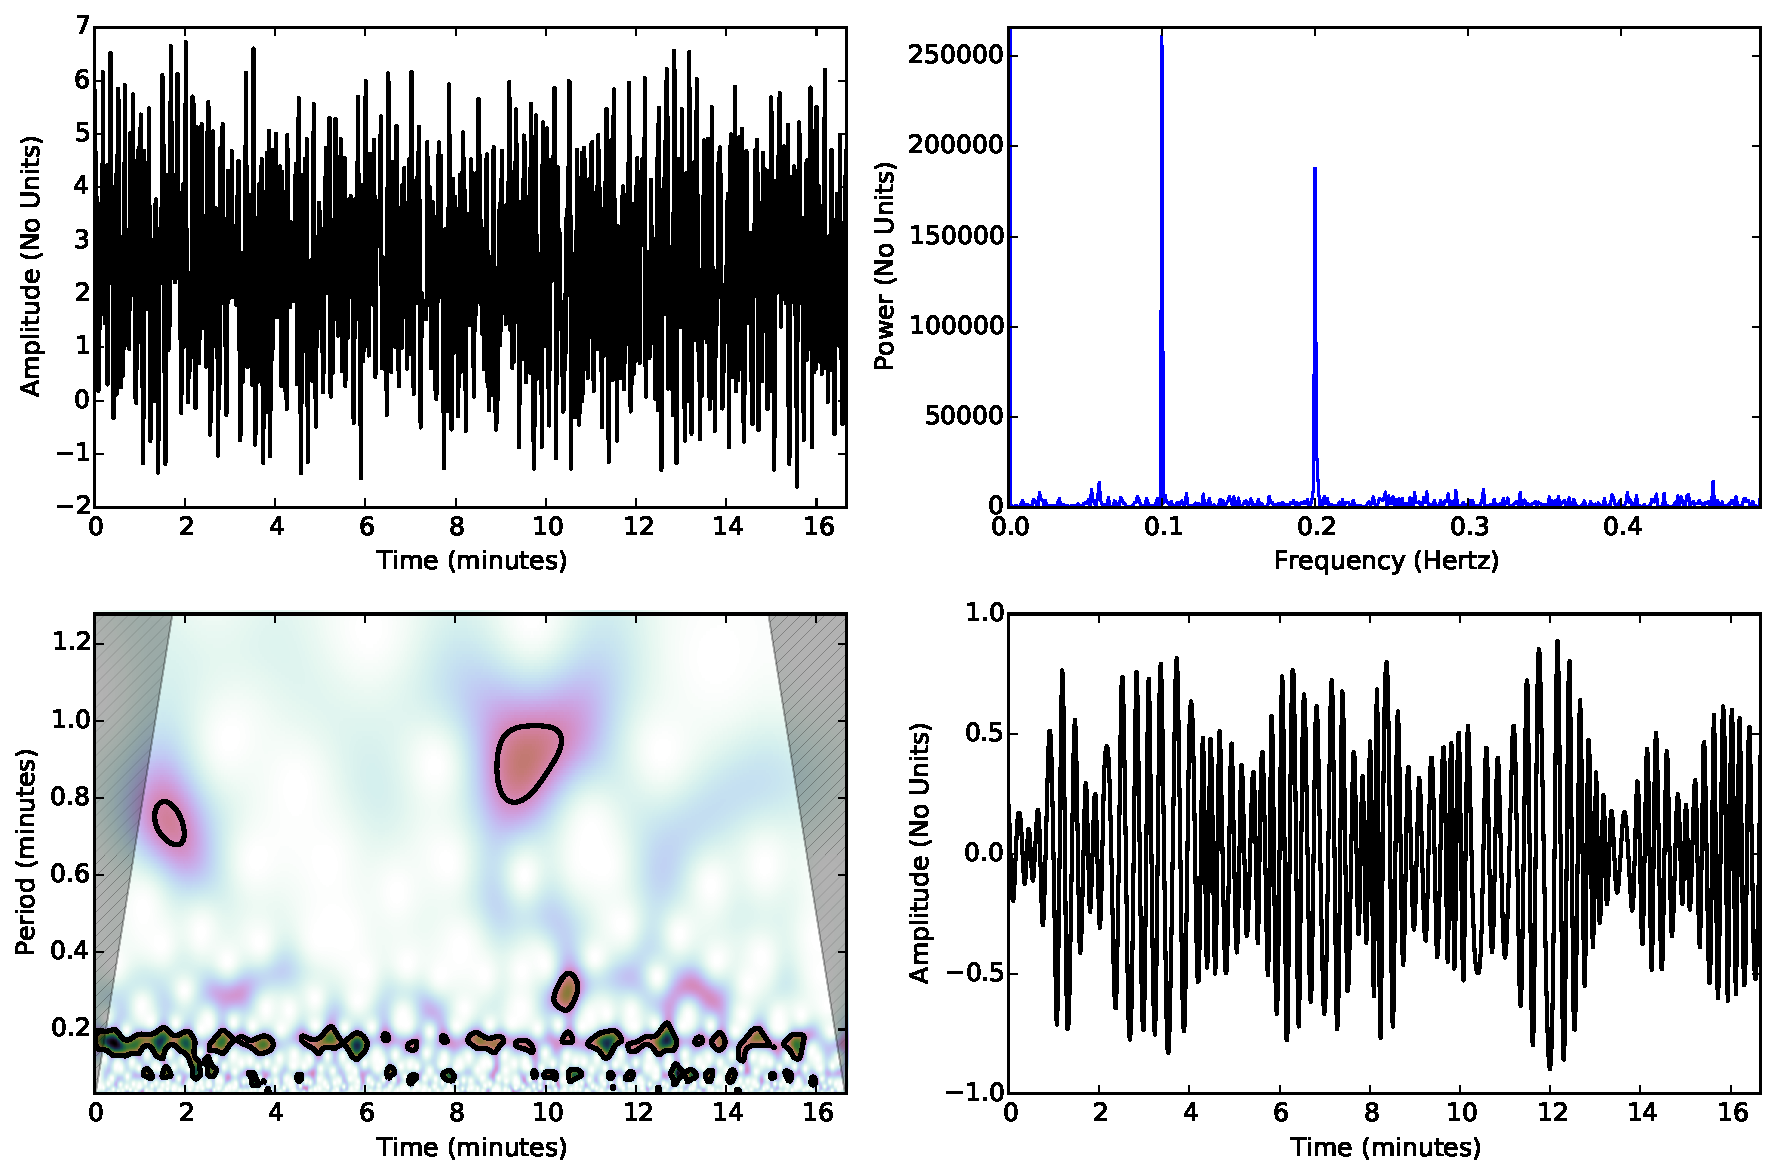
\includegraphics[width=0.85\textwidth]{signal_overview.pdf}
           \caption{
                   An example of the signal analysis methods. 
                   The upper left plot is of an artificial signal with noise.
                   The upper right plot is a power spectrum from the FFT.
                   The largest two peaks shows the frequencies within the artificial signal.
                   The bottom left plot is a wavelet power spectrum.
                   It expands on the FFT by offering a 2D view of the frequency spectrum with time.
                   The bottom right plot shows an IMF output from a EMD algorithm.
                   The IMF contains one of the periods from the artificial signal used and this corresponds to the smaller frequency within the artificial signal.
                   }
              \label{fig:signal_overview}
     \end{sidewaysfigure}
	
	The nature of signal analysis means that each individual method has both positives and negatives.
	Generally, the type of signal or the overall aim will determine the method used.
	To start, input signals have a finite length and many signal analysis methods assume infinite length, which is the case for the Fourier Transform. 
	This fact means that artefacts are introduced as a result, however, this is not unique to the FFT and most signal analysis algorithms suffer from this issue. 
	The FFT has an effect known as frequency leakage.
    It is where, if the input signal is non-periodic or the input signal has no closed form transform, there is smearing in the power spectrum.
    This means that the power is not confined to the correct frequency and spreads, so if there is an other frequency close to a strong frequency, it will be masked.
	This can be overcome by using a window function, through a process called windowing. These window functions are non-zero in a chosen interval and are then multiplied to the original signal before it is then put through the FFT.
	The shape of these window functions varies and numerous windows have been created. 	
	This alters the outcome of the FFT in order to reduce the effects of spectral leakage.	
    Furthermore, another important part of the FFT is the output can be reversed.
    It is possible to recover the original signal using the Inverse FFT (IFFT).
    This fact means that one can create a bandpass filter and apply it to the Fourier space.
    This is done in order to remove parts of the Fourier space that contains information that is unnecessary and thus return a new signal to see the behaviour at specific frequencies.
    It is a commonly used method in signal analysis and is used within Chapter 5.
    
    Finally, the significance of the FFT power spectrum is an important factor, since it is vital to establish if the periods are above noise level.
    While there are numerous methods to achieve this, here is a brief overview of just two.
    The first method is described by \cite{1982ApJ...263..835S} and \cite{1986ApJ...302..757H}.
    It relies on normalising the power spectrum and assumes that the noise in the data is truly random. 
    This means that the probability of the noise at any given frequency being above a power value, $z$, is exponentially distributed, scaling as $\exp(-z)$.
    This defines the ``false-alarm probability'' at which a given power is equal to, $1 - (1 - \exp(-z))^{N_i}$, where $N_i$ is the number of frequencies contributing to the power spectrum.    
    The second method is a Monte-Carlo method known as Fisher Randomization.
    Given a signal, the FFT of the data is calculated and the power of the highest peak is determined.
    Then the original signal is then randomly permuted and the FFT is re-calculated. If the highest peak in the new FFT is higher than that of the original, `1' is added to the count.
    The process is repeated the desired number of times and the false alarm probability is returned at the end and it is simply the count divided by the number of permutations \citep{1985AJ.....90.2317L}. 
    
\subsection{Wavelet transform}

	The second method employed is called the Wavelet Transform.
	A wavelet is a zero mean function that is constrained in time and frequency space i.e., localised within these specific domains \citep{farge1992wavelet}.
	The base function used is called the mother wavelet and variations of this function are called daughters.
	This factor is important, as the FFT will, when given a 1D signal, output a 1D power spectrum.
	The wavelet algorithm will return a 2D spectrum where the extra dimension is time.
	This means you can also know what frequency is within the signal but also at what time in the signal that frequency exists and its duration.
	This is a more powerful method due to this fact, but also, each mother wavelet have different properties so depending on the goal of the signal analysis, by changing the mother wavelet different information can be extracted. 
	For example, the wavelet chosen here is the Morlet Wavelet.
	It is defined as,
	\begin{equation}
		\Psi_0(\eta) = \pi^{-1/4} \exp(iw_0\eta)\exp(-\eta^2/2),
	\end{equation}
    where $\eta$ is a non-dimensional time, $w_0$ is the non-dimensional frequency.
    This can be summarized as a plane wave modulated by a Gaussian.
	It has good frequency resolution but it comes at a cost of its time resolution, while another wavelet called the Paul wavelet has a poorer frequency resolution but it has an increased time resolution.
	This allows the wavelet transform to be manipulable to the users' goal.
    
    From this step, the continuous wavelet transform can be defined as the convolution of each data point with the scaled version of $\Psi_0(\eta)$,
	\begin{equation}
		W_n (n, s) = \sum_{n^\prime}^{N-1} x_{n^\prime}\Psi_{0}^{*} \left[\frac{(n^\prime-n)\delta t}{s}\right],
	\end{equation}
    where $s$ is the wavelet scale, $x_n$ is the data point at time index $n$, where $\delta t$ is the time step and where $*$ means the complex conjugate. 
    Thus by varying the wavelet scale and moving along the time index, it becomes possible to construct an image showing both the amplitude of any features versus the wavelet scale and how this amplitude varies with time. 
    It should be noted that the wavelet scale will need to be transformed into frequency, but for the Morlet wavelet the wavelet scale is proportional to the frequency.
    
    The bottom left image of Figure \ref{fig:signal_overview} shows the output of a wavelet algorithm on the artificial signal.
    The dark regions show an increase in the power, which shows where the periods of the signal are.
    The wavelet algorithm has the ability to calculate the significance of any regions of power and the black contour lines show this.
    The contour lines shown are for 95\% significance. 
    Further, much like the FFT, the finite length of a signal creates edge effects for the wavelet.
    This can be seen as the cross-hatched regions, these mark the region where the finite length of the signal affects the wavelet transform.
    This is called the cone of influence (COI) and it is different for each mother wavelet.
    
    Finally, the wavelet transform allows for direct comparison of two signals.
    It is possible to calculate the cross-wavelet of two signals as well as the correlation and the phase difference using the wavelet transform.
    This fact allows the wavelet transform to be used to measure the phase difference of the cross-sectional area and total intensity signals, which is the main method used to find the phase difference.
    This is possible with the FFT. 
    However, due to the localised nature of the wavelet transform, the phase difference can found as  a function of frequency and time.
    Thus it is possible to see if the phase difference varies for that frequency which could indicate an underlying physical mechanism such as mode conversion for the observed waves.
    See \cite{torrence} for an overview of the wavelet transform and its applications.
    Further, see \cite{2004SoPh..222..203D} and \cite{WAUO} for an overview of wavelets in a solar physics context.
    
\subsection{Empirical mode decomposition}

	Finally, we have the Empirical Mode Decomposition (EMD).
	As the name suggests, this method is not based off a mathematical theorem or transformation in the way that the FFT or wavelets.
    The algorithm will output several signals, called the residual and Intrinsic Mode Functions (IMFs).
    The residual is the left over signal from the algorithm and tends to contain any slow varying background trend.
    An IMF will generally be a simple oscillatory mode, ideally it should contain one of the frequencies within the original signal.
    There are two requirements in order to be considered as an IMF.
    Firstly, the number of extrema and zero crossings must either be equal or differ by one.
    Secondly, the mean value of the envelope defined by the local maxima and the envelope defined by the local minima equals zero.
    This means that the output from the EMD is constrained, which results in non-arbitrary signals.
    
    The steps of the algorithm are as follows,
    \begin{enumerate}
        \item The local minima and local maxima of the input signal are found.
        \item A spline fit of the minima and maxima points is computed.
        \item The resulting minima and maxima curves create an envelope that encompass the signal.
        \item The mean of the envelope is subtracted from the input signal and this process is repeated again. This is termed sifting.
        \item The sifting stops once the stopping criterion is satisfied.
        \item The resulting signal is called an IMF and is subtracted from the original signal. The leftover signal is termed the residual.
        \item This process repeats itself again on the residual signal until a set number of IMFs are obtained or the residual signal contains too few extrema to spline fit.
    \end{enumerate}
    These steps are shown in Figure \ref{fig:EMD}.
    There are three comments to be made here about the algorithm.
    First, a local minima (maxima) point is defined if that point is smaller (larger) than its two neighbouring points.
    Second, are two commonly used definitions for the stopping criterion.
    The first one is, if the standard deviation of the sifted signals is lower than a given limit, which is typically less than 0.3, the process stops.
    The second one is called the S number which is, if the same signal is returned by the sifting process more than S times, this causes the process to stop.
    Thirdly, the overall algorithm has no method of deciding when enough IMFs have been found, so the number picked is arbitrary, but generally the algorithm will stop before this limit is reached.
    This is because as the residual becomes linear with each IMF removal, the fitting algorithm will stop naturally since there is not enough extrema points to spline fit.

   	\begin{figure}
   		\centering
   		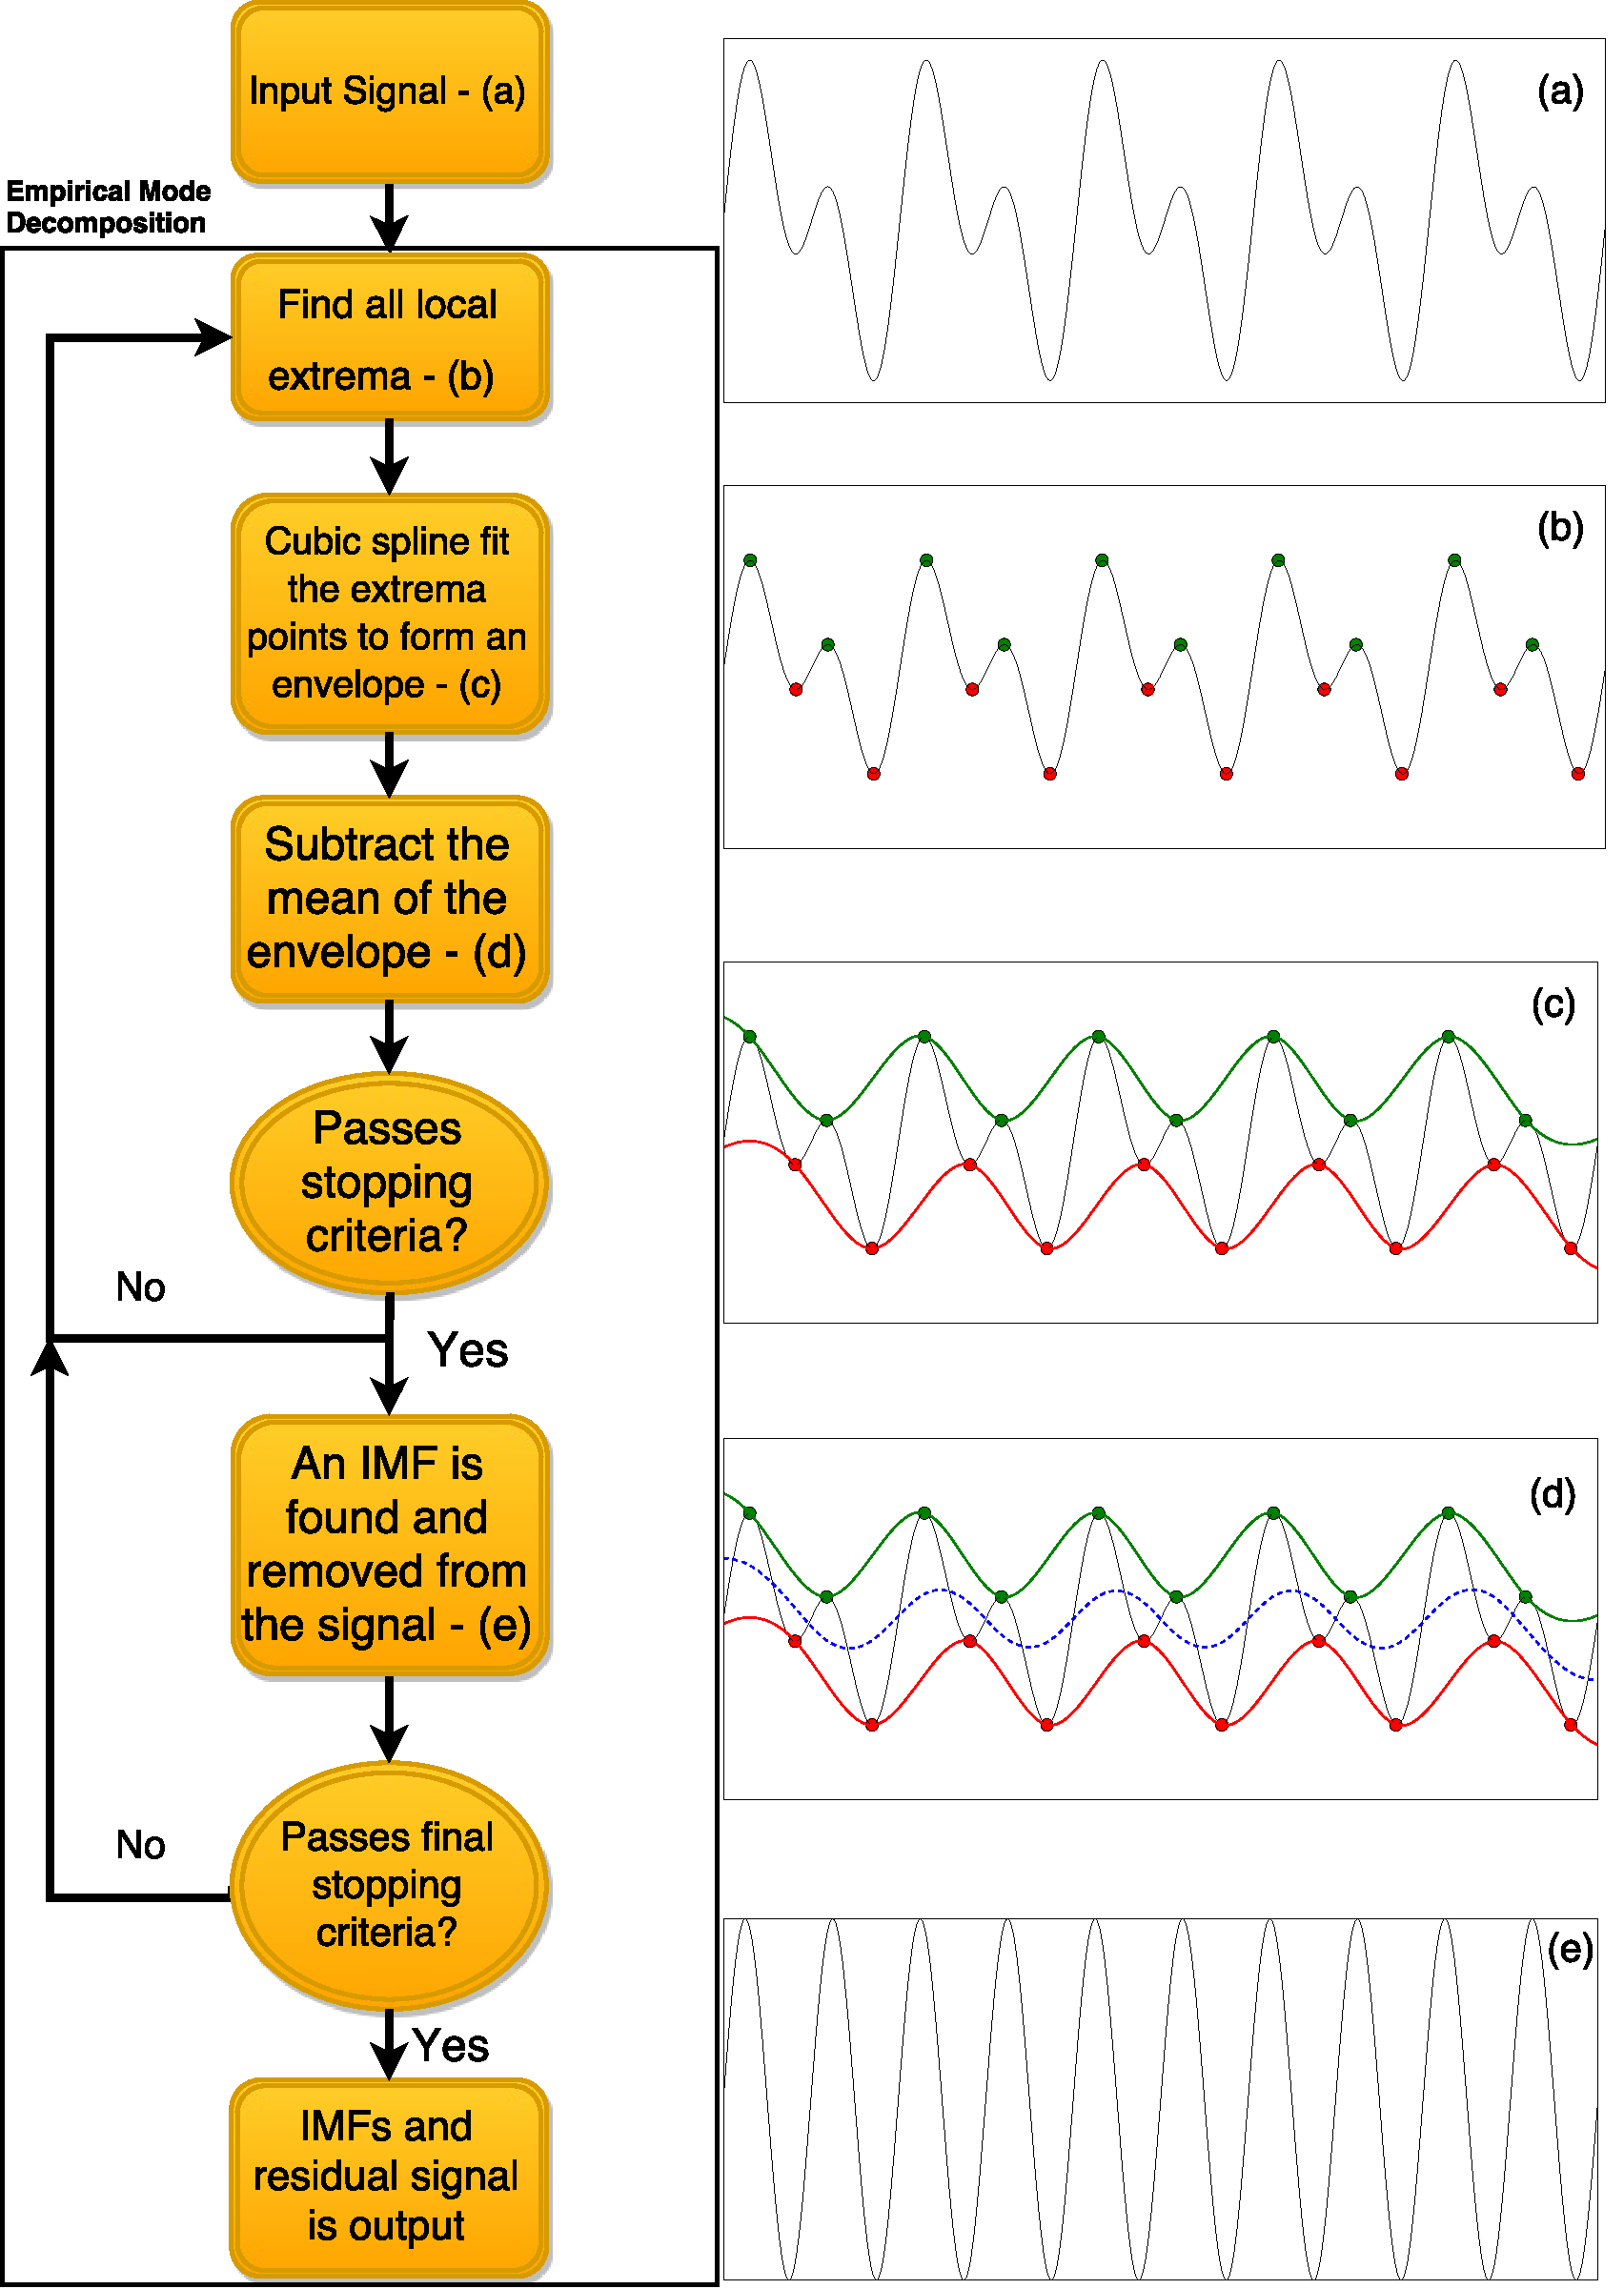
\includegraphics[width=1\textwidth]{EMD_FLOW.pdf}
   		\caption{
   			     An overview of the steps that form the Empirical Mode Decomposition (EMD) algorithm. 
   			     On the left is a flow chart that summarises each step of the EMD algorithm.
   			     On the right is a graphical explanation of certain steps in the flow chart. 
   		        }
   		\label{fig:EMD}
   	\end{figure}
   	    
    The resulting set of IMFs, contain the periods within the original signal, while the residual should contain any background trend.
    Much like the FFT, you can reverse the method as the sum of all of the IMFs and residual will return the original input signal.
    The EMD allows much like the cross-wavelet, the ability to find the phase difference between two signals containing the same periods.
    With a direct comparison of the IMFs of one signal to another, you can measure the phase difference between them and was carried out by \cite{morton2011}.
    The EMD algorithm is also very good at separating noise from a signal, which is what the first IMF generally contains.
   
    The drawbacks for the EMD are most focused on the method, since it has no mathematical foundation like the FFT or wavelet.
    The most important issue for the EMD is the spline fit that creates the envelopes.
    The envelope fit with each iteration, starts to become very large at the edges since there is nothing to constrain it.
    As such, when these are subtracted from the signal, the resulting IMFs display large swings at the start and end, so these edge effects will easily affect the output.
    To counter-act this effect, several methods have been suggested to lessen this issue and it will generally involve adding extra extrema points on both sides to constrict the spline fit \citep{zeng2004simple}.
    See \cite{huang} for an detailed overview of the EMD and \cite{terradas} for a solar physics context.

\subsection{Multiple methods}    

    Within this thesis, three different signal analysis methods are utilised.
    Overall, the main idea was to confirm the results of each analysis method.
    While each individual method offers the ability to find a periodicity within a signal and to compare the phase of two signals. 
    On their own, they offer no independent verification that the found periodicity and phase is correct. 
    But using the other methods it allows each method to be verified before any conclusions can be made.
    Each method has its own strengths and flaws and by using all three, it is possible to take account of any flaws.
    The FFT offers a snapshot interpretation of a signal, as the output is only a function of frequency. 
    However, the wavelet and EMD offer the ability to examine how a periodic changes as a function of time as well.
    This allows for a more detailed interoperation than the FFT.  
    Furthermore, the wavelet transform does not cope well with noise in the high frequency part of the spectrum and this can be seen clearly in bottom left image in Figure \ref{fig:signal_overview}.
    The smaller frequency component have been found by the wavelet but it is not continuous through time, while the higher frequency component has been detected less.
    Without the noise in the signal, or a higher signal to noise ratio, the wavelet gives a much better representation of the input signal. 
    The output of the EMD detects both periods without an issue but it has not returned the correct amplitude due to the noise in the original signal. 
    Thus the EMD excels for detected high frequency components over the wavelet, especially for noisy signals.
    The main issue with the EMD algorithm is the detection of low frequency components, as the algorithm iterates further, the edge effects can become a problem.
    As a result, the low frequency components in a signal can become washed out from an IMF. 
    The wavelet does not have a problem with low frequency components, even for noisy signals. 
    In conclusion, the combination of these three signal analysis methods allows the weakness of one method to be overcome with another and allows each result to be checked.
  
\section{Area analysis}

	The core idea behind the work presented in this thesis is analysing the cross-sectional area of pores and sunspots.
	So it is vital to be able to confidently measure the cross-sectional area.
    The base idea is to threshold the structure and use that as a measure of its cross-sectional area.
    The issue is that various methods have been used in published research.
    While many never state exactly how they contoured a sunspot or a pore, partially due to not caring explicitly about the cross-sectional area.
    Previously, \cite{morton2011} used a $2.5\sigma$ threshold of the mean background intensity for G-band data, here, sigma ($\sigma$) refers to the standard deviation of the background intensity.
    The number before sigma will be called the sigma multiplier throughout this section.
	More recently, \cite{0004-637X-806-1-132} used $2.2\sigma$ of the mean background intensity for their data.
    This was to account for the change in contrast between several different wavelength filters as this was the first multi-height analysis.
    Their aim was to measure the cross-sectional area of a pore from the photosphere to the lower chromosphere which is challenging topic.
	
	What will occur in this section is an analysis on the effect of changing the sigma multiplier on the returned cross-sectional area signal.
    The value of sigma can appear to be arbitrary and there is an assumption that the intensity of the background photosphere has a normal distribution and as such, sigma can be used to contour these magnetic structures.
    To be more precise, whether different sigma values will give different periods after signal analysis or if the value of sigma once set within a certain range does not change the output is of interest.
    This will be discussed in this section.
    Furthermore, since the current selection of ground-based solar telescopes have resolutions similar to each other and this could be the limiting factor in detecting these oscillations.
    As the slow MHD sausage mode affects the cross-sectional area much less than the fast MHD sausage mode, it is most likely mode to be detected in observations.
    
	This analysis is only for ground-based data and for ion lines that sample the photosphere directly.
	The chromosphere lines used traditionally (\ion{Ca}{II} and H$\alpha$ line core) make resolving the fine boundaries of a sunspot or a pore very difficult.
	The cross-sectional area and total intensity are inherently linked on a conceptual level.
	Thus, it might be possible that if the intensity changes, a fake period could be introduced into the cross-sectional area.
    Furthermore, during ground observations the light level will change or the seeing conditions will vary, this could introduce an artificial period into the cross-sectional area and total intensity signals.
    Figuring out how to account for these effects will be important, however these are areas for future investigation.
    
    \subsection{Data}
    
    The data for this investigation comes from two instruments on the DST: IBIS and ROSA.
    The IBIS dataset consists of an image series of a H$\alpha$ line scan.
    The DST was centred on a sunspot in AR 11579.
    The observation run was on the 30$^{\mathrm{th}}$ of September 2012 at 15:00 UT until 15:16 UT with a cadence of 6.8 seconds.
    The full field of view (FOV) was 96\arcsecs by 96\arcsecs with a pixel size of 0.097\arcsecs.
    The part of the line scan used here is -0.7 nm, which falls into the blue wing of the H$\alpha$ line profile.
    This part of the line profile samples the photosphere strongly and will show Ellerman Bombs as well as Type II spicules.
    See \cite{2013A&A...560A..31N} on the reduction methods for this IBIS dataset.

    The ROSA dataset consists of an image series of G-band narrowband filter images.
    The DST was centred on a small pore cluster in AR 11683.
    The observation run was on the 6$^{\mathrm{th}}$ of March 2013 at 19:27 UT till 20:02 UT with a cadence of 2.11 seconds.
    The full FOV was 115\arcsecs by 115\arcsecs with a pixel size of 0.12\arcsecs.
    The narrowband filter means that only the line core was sampled and for G-band (430.5 nm) this corresponds to the low photosphere.
    See \cite{0004-637X-806-1-132} for the reduction methods for this ROSA dataset.
    
    Both magnetic structures can be seen in Figure \ref{fig:data_overview}.
    The image on the left showcases the  IBIS sunspot while on the right, the ROSA pore is displayed.
    Both images are context images and do not show the full FOV of each instrument during that observation run.
    Both structures are stable throughout their respective observation run.

    \begin{sidewaysfigure}
        \centering
        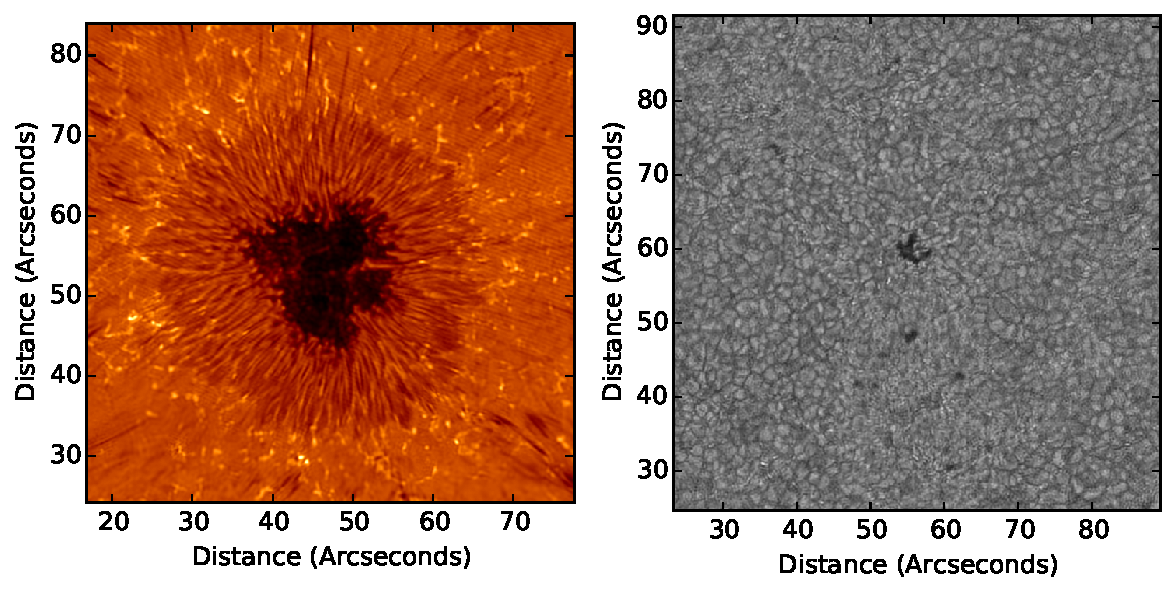
\includegraphics[width=\textwidth]{overview.pdf}
        \caption{
                The left figure is the cropped field of view (FOV) for IBIS.
                It is in the blue wing of the H$\alpha$ line profile which samples the photosphere and not the chromosphere that the line core samples.
                The sunspot is in AR 11579 and was taken on the 30$^{\mathrm{th}}$ of September 2012 at 15:00 UT until 15:16 UT.
                The right figure is of a cropped FOV for ROSA.
                It is the G-band narrowband filter which samples the lower photosphere.
                The focus is on a small pore cluster, in AR 11683 and was taken on the 6$^{\mathrm{th}}$ of March 2013 at 19:27 UT till 20:02 UT.
                The pore investigated is the larger one in the middle.
                }
        \label{fig:data_overview}
    \end{sidewaysfigure}
    
    \subsection{Method}
        
    The method used to contour these structures is as follows.
    The starting point is to find a large region of the quiet Sun photosphere, where there is no strong magnetic features.
    This area is used to calculate the mean intensity and a histogram of this area should form an approximate normal distribution.
    The normal distribution means that the standard deviation can be used to select specific pixels within the image.
    As the number of standard deviations is increased, more of the data will be covered by the distribution.
    By limiting the pixels of interest by having a limit that is lower than say two standard deviations or higher, the pixels left over will be the darkest 5\% of pixels, or the other way round would return the brightest 5\% of pixels.
    Theoretically, the lower limit should return the pixels for sunspots and pores which are substantially darker than other features in the photosphere.
    By counting these pixels, this should correspond to the cross-sectional area of these magnetic structures.
    
    Figure \ref{fig:method_overview} shows this method applied to these datasets.
    The left column shows the context images of each dataset shown in Figure \ref{fig:data_overview}.
    However, added to these images are four contours coloured as follows: blue, green, purple and orange.
    Each colour represents a different sigma multiplier for the standard deviation.
    The sunspot and pore do not share the same range of sigma multipliers.
    For the sunspot the sigma multipliers are 3, 3.5, 4, 4.5 and for the pore they are 2, 2.5, 3, 3.5.

    \begin{sidewaysfigure}
        \centering
        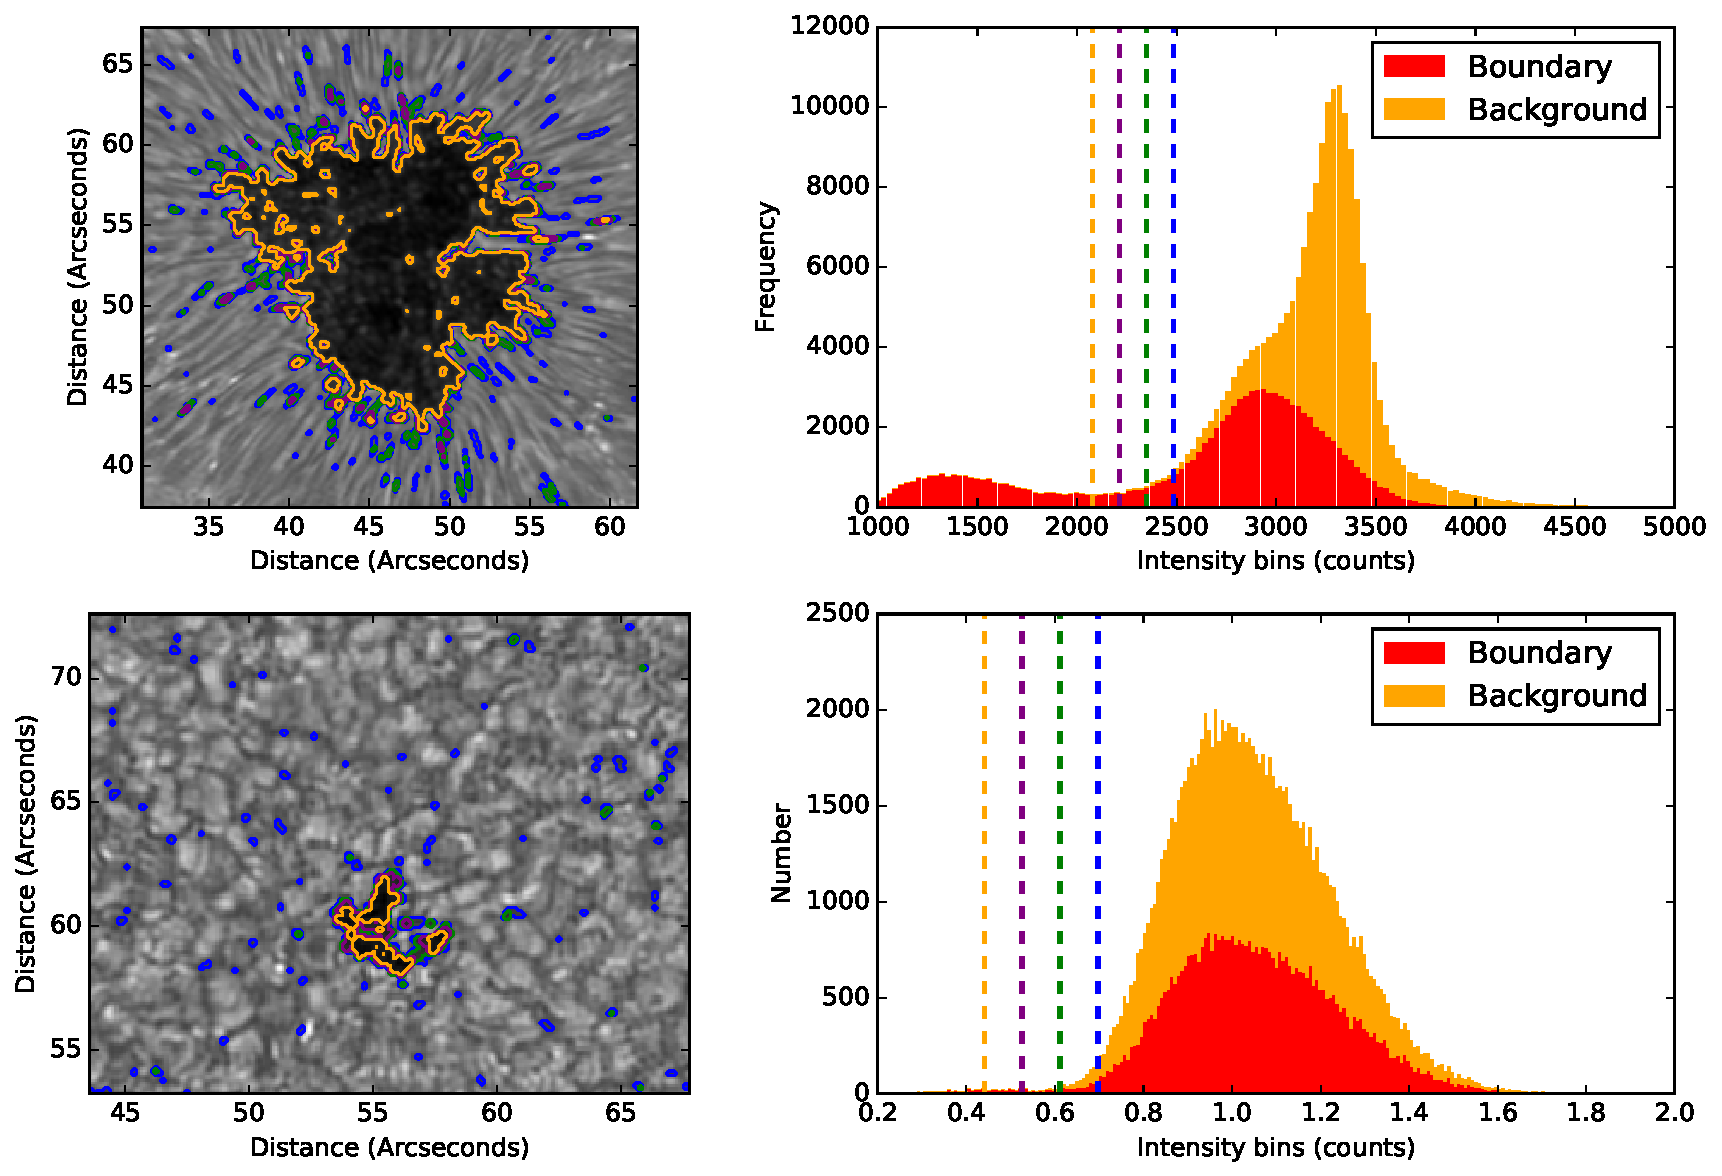
\includegraphics[width=0.85\textwidth]{method_overview.pdf}
        \caption{
                An overview of the method used to contour magnetic structures.
                The left column shows context images of the datasets shown in Figure \ref{fig:data_overview}.
                They have the contours of the various sigma multipliers shown.
                The contour colours of blue, green, purple and orange correspond to 3, 3.5, 4 and 4.5 and 2, 2.5, 3 and 3.5 for the sunspot and pore respectively.
                The right column shows histograms of the background photosphere in yellow and of the context image shown on the left in red.
                The vertical lines shown display where the sigma multipliers end up on the histogram.
                }
        \label{fig:method_overview}
    \end{sidewaysfigure}
    
    \subsection{IBIS sunspot}
    
    The contouring for the sunspot at the lower sigma multipliers does capture small parts of the penumbra.
    For example at 2.5$\sigma$ (which is not shown), the contour was the entire sunspot, i.e., the umbra and penumbra.
    The jump to 3$\sigma$ (blue) curtails most of the penumbra.
    Once sigma is at 3.5 and 4, which correspond to the green and purple contours, the penumbra that is contoured has shrunk nearly to zero.
    However, it is not until we reach the largest sigma value, 4.5 which is the orange contour, that the penumbral area disappears completely.
    The reason for this can be seen in the right column of Figure \ref{fig:method_overview}.
    The top figure is of a histogram of both the background which is in yellow and the context image on the left which is in red.
    The background here is not a normal distribution and the reason for this is that the full FOV does not have a good area of quiet Sun photosphere.
    The wings of H$\alpha$ show a variety of features, including Ellerman Bombs and Type II spicules, so finding an isolated region becomes harder.
    Furthermore, the full FOV is more limited in IBIS than ROSA or CRISP. 
    This means that the sigma value is skewed and thus the sigma multiplier will have to be higher to counter act this.
    Finally, the sunspot histogram shows a clear difference between the penumbra and umbra.
    The histogram can be split into two parts, the left part contains the umbra and the right part contains the penumbra.
    The penumbra for this sunspot occupies a larger portion of the context image which explains why the right part of the histogram is taller, i.e., a higher count.
    At the intensity values between 1800 to 2300, the histogram plateaus and within this region is where the range of sigma multipliers lie. 
    The vertical coloured lines correspond to the same colour contour lines in the context image.
    It is possible to claim that, as long as the sigma multiplier is in between this range, we have isolated the penumbra from the umbra.
    Using this as guide, it makes it easy to show that the sigma multiplier of 4.5 (orange) would be an ideal value since it gives a value in the middle of the plateau.
    
    \subsection{ROSA pore}
        
    The overall picture is quite different and the main reason for this is the lack of a penumbra.
    While there was a plateau that separated the penumbra and umbra for the sunspot, this is missing for the pore and the sigma multiplier is harder to choose directly.
    The sigma multipliers are lower for the pore and are 2, 2.5, 3 and 3.5.
    Each of these are shown on the bottom left image of Figure \ref{fig:method_overview}.
    These values again correspond to blue, green, purple and orange contours.
    The lowest multiplier contours large amounts of the background photosphere.
    However, all the larger multipliers contour only the pore.
    There are clear parts of the pore that are ignored with these higher multipliers.
    By looking at the histogram, a different picture emerges when compared to the sunspot.
    Since the pore is very small, the behaviour of the previous histogram for the sunspot does not emerge.
    There is no clear separation between the background and the pore, so picking a direct sigma value is more difficult when using the histogram.
    The background histogram also has a normal distribution unlike the IBIS sunspot.
    The lower limit (the blue vertical line) shows that at this value, there is still large amounts of the background quiet Sun.
    But, as the limit is increased, that amount drops to near zero and as such, we have very little quiet Sun within the cross-sectional area contour.
    Here, instead of a plateau, the histogram reveals that there is a tail.
    This tail corresponds to the pixel values that correspond to the pore and it can be used to pick a sigma multiplier since it tails off to much lower values than the quiet Sun histogram.
    The start of this tail is around 2.5$\sigma$ and this gives a very good contour of the pore.
    That is why taking values of the threshold above 2.5$\sigma$ cuts off pixels that are clearly part of the pore.
    The different sigma multipliers used for the sunspot and pore are most likely due to the lack of a good background region for the sunspot in IBIS.
    A direct comparison of intensity counts for a sunspot and pore is difficult since the ROSA pipeline normalizes the intensity counts.
    
    \subsection{Discussion}
    
    Finally, it is important to see whether these different sigma multipliers give different periods within the resultant cross-sectional area signals.
    Figures \ref{fig:sunspot_wavelet} and \ref{fig:pore_wavelet} show the wavelet transform of the signals that correspond to the smallest and largest sigma multipliers used for the sunspot (3, blue and 4.5, orange) and pore (2, blue and 3.5, orange).
    The top row show the cross-sectional signals of these sigma multipliers and the bottom row is the resultant wavelet transforms.

    \begin{sidewaysfigure}
        \centering
        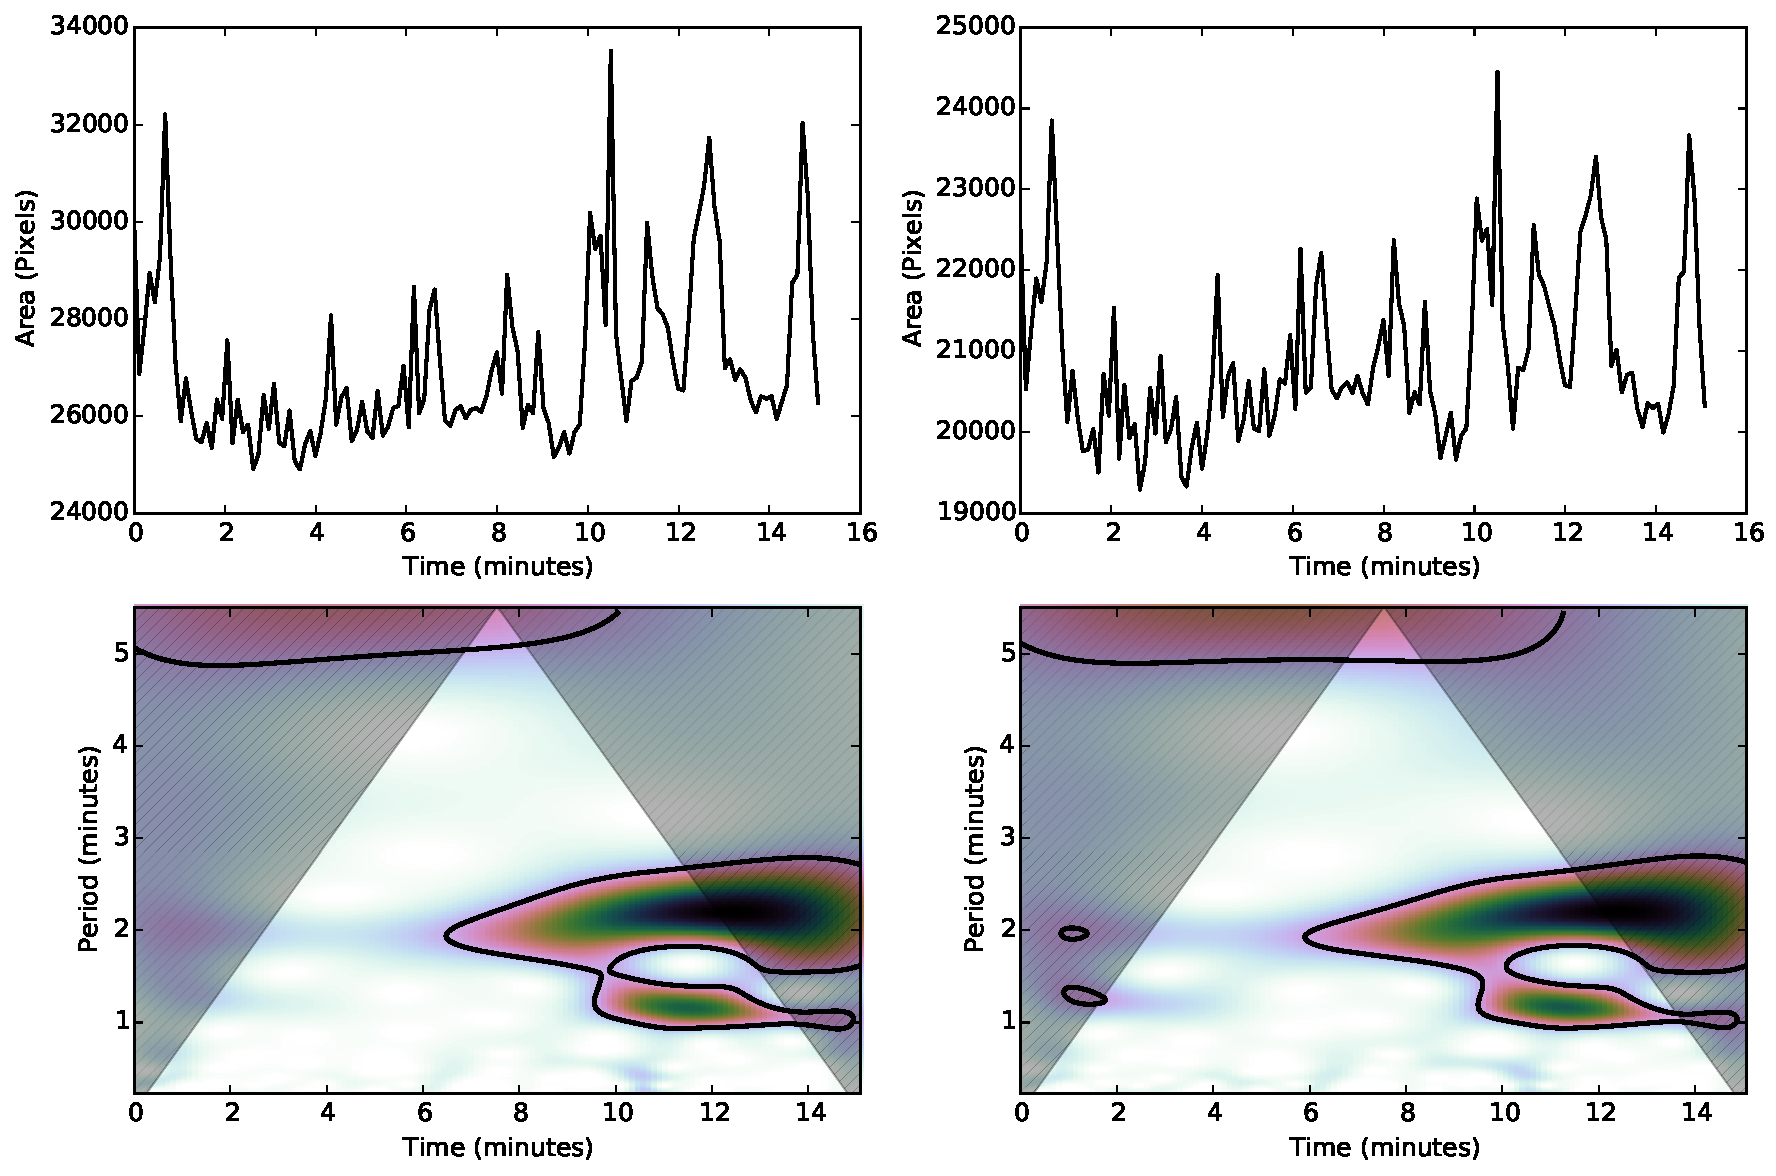
\includegraphics[width=0.75\textwidth]{sunspot_wavelet.pdf}
        \caption{
	             The top row shows the cross-sectional area signals returned from a sigma multiplier of 3 and 4.5 for the IBIS sunspot.
	             These correspond to the blue and orange contours in Figure \ref{fig:method_overview}.
	             The bottom row shows the resultant wavelet transform of these two signals.
	             The cross-hatch region is the cone of influence, while the black contour line is the 95\% significance level.
	             The returned wavelet transforms images show that for the IBIS sunspot, the difference in sigma multipliers cause no variation in the detected area oscillations.
                }
        \label{fig:sunspot_wavelet}
    \end{sidewaysfigure}
    
    \begin{sidewaysfigure}
        \centering
        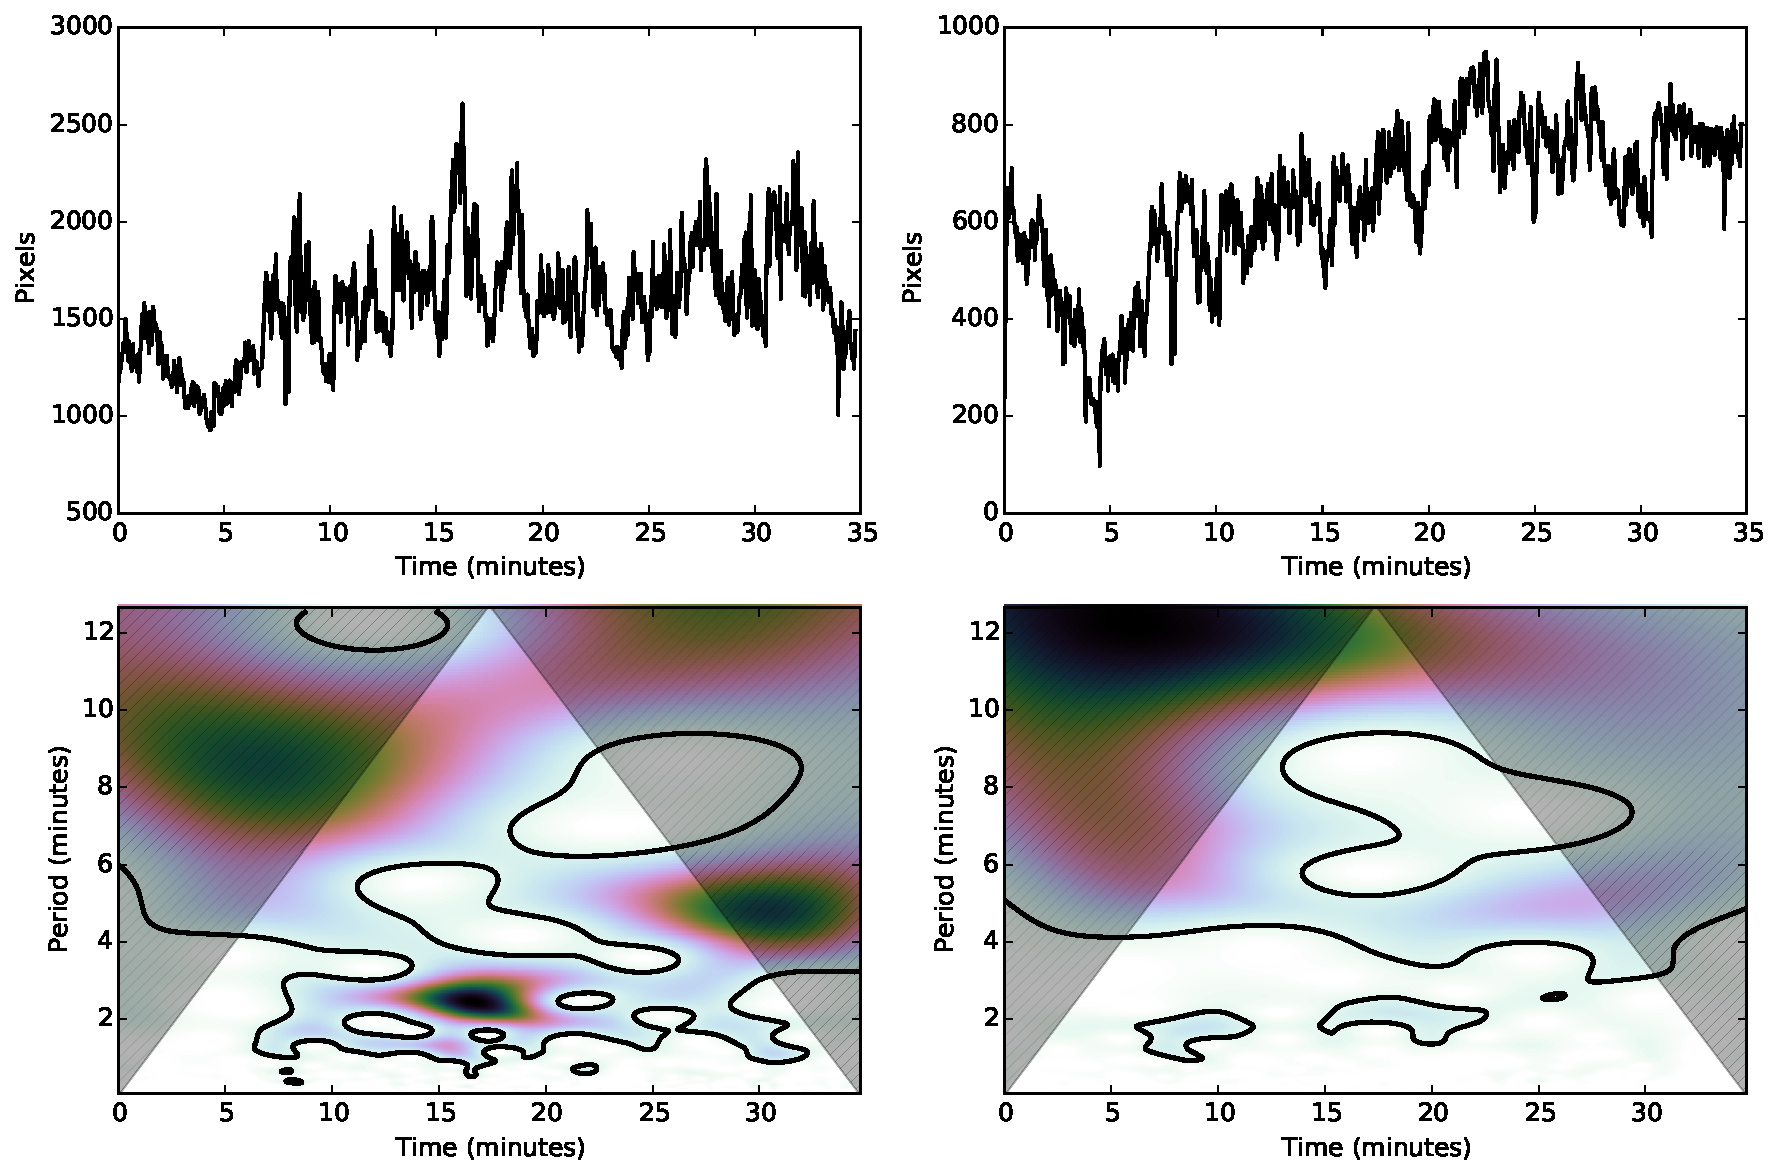
\includegraphics[width=0.75\textwidth]{pore_wavelet.pdf}
        \caption{
		         Same as Figure \ref{fig:sunspot_wavelet} but for the ROSA pore.
		         The lowest sigma multiplier is 2 and the largest is 3.5. 
		         These correspond to the blue and orange contours in Figure \ref{fig:method_overview}.
		         Unlike the sunspot, there is a clear difference between the different sigma multipliers.
		         The periods at 2 and 3 minutes are not shown in the largest case and this showcases that for pores, the sigma multiplier is very important. 
                }
        \label{fig:pore_wavelet}
    \end{sidewaysfigure}
    
    The IBIS sunspot shows little change between the sigma multipliers.
    Since the range of sigma multipliers correspond to the plateau region, the returned cross-sectional area does not catch the penumbra, so the signal that corresponds to either one is focused heavily on the umbra and detects the periods found in the umbra.
    Thus, for this range of sigma multipliers, the same periods are found within this dataset.
    The short length of this data series means that it is impossible to find larger period oscillations, so the only periods found in this sunspot are 1 and 2 minute oscillations.
    This is interesting, since it should be possible to observe 3 and 5 minute oscillations but they are absent within this particular dataset.
       
    Now, for the pore observed in ROSA.
    To start, it is important to note that it is a longer observation sequence.
    The most obvious difference here is the variation of wavelet power at periods less than 4 minutes between the two sigma multipliers. 
    For the lowest sigma multiplier (2, blue), there is a large amount of wavelet power and most of that region is above the significance level. 
    This image is the opposite for the largest sigma multiplier (3.5, orange).
    There are only two small regions of wavelet power that are within the significance level.
    Otherwise, the difference between these sigma multipliers is minor.
    These are for the larger periods that can be seen at 5 and 9 minutes.
    While they are under the cone of influence, they are more obvious and their associated wavelet power is larger for the smaller sigma multiplier.
    However it important to note that both sigma multipliers still have the same oscillation periods.
    The cause of this difference is that the larger sigma multiplier undersamples the pore and this has caused the large difference observed in the wavelet figure, as one might expect.
    However, this reveals that the difference here is still minor, it would matter most if the wavelet power was used to measure the amplitude of these oscillations.

	Finally, ending on mode identification.
	Figures \ref{fig:phase_sunspot} and \ref{fig:phase_pore} show the cross-wavelet phase diagram between the cross-sectional and total intensity signals for the IBIS sunspot and ROSA pore, respectively.
	The output is in the same style as the normal wavelet, however, the colour indicates the phase difference in degrees, where blue is positive and red is negative degrees.
	By checking the regions where the cross-sectional and total intensity wavelets overlap, it is possible to see what the phase difference is.
	In this case, for both magnetic structures the phase difference is strongly in phase. 
	The ROSA pore demonstrates a more complex image, there are more regions of out of phase behaviour that seems to change from positive to negative.
	However, the regions with this behaviour are smaller than one wave period and are ignored as a result.    
	This behaviour is more common in pores than sunspots.
	Overall, within both these structures the oscillations can be classified as slow MHD sausage modes. 
	It should be noted that this study does not fully cover every nuance regrading this method, it is something that is discussed in Chapter 6.   
	In conclusion, as long as the value of sigma multiplier is sound, the sigma multiplier will not vary the result.
	    
	\begin{sidewaysfigure}
    	\centering
    	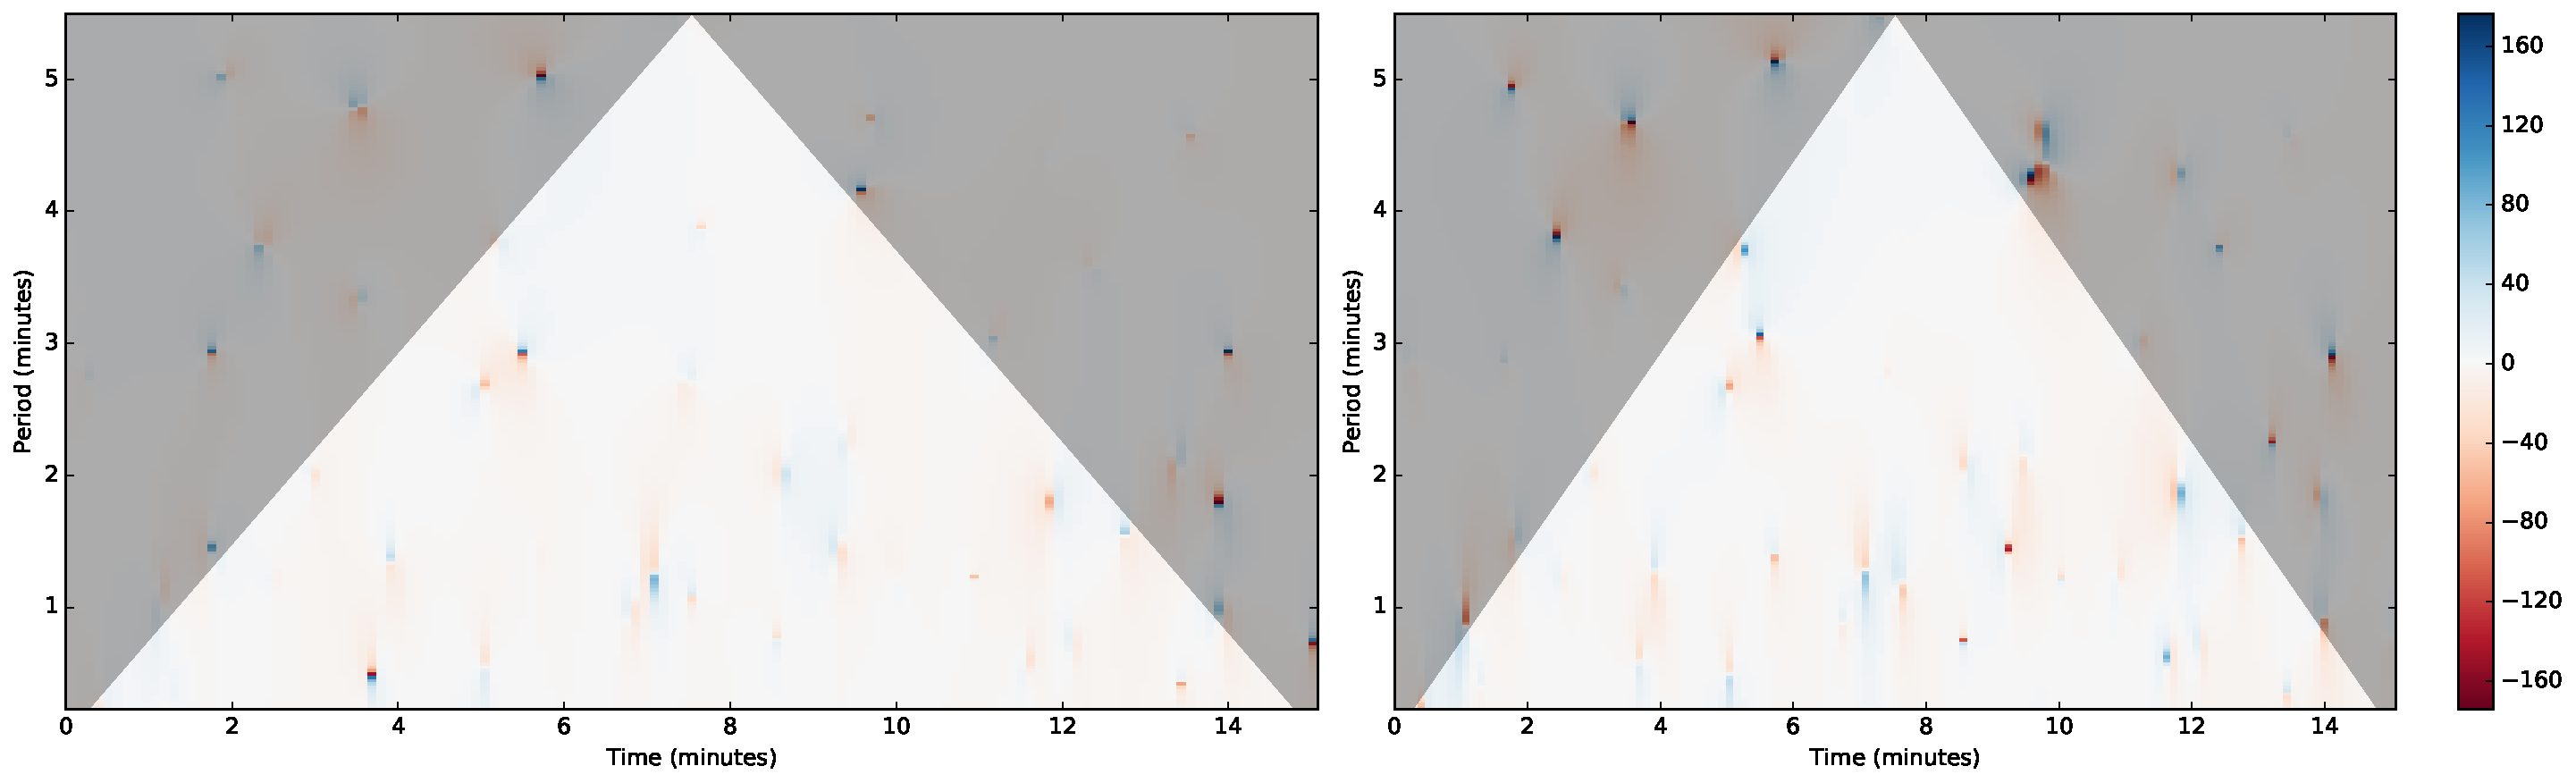
\includegraphics[width=1\textwidth]{sunspot_phase.pdf}
    	\caption{
			            The wavelet phase difference between the cross-sectional area and total intensity for the IBIS sunspot.
			            The lowest sigma multiplier is 3 (left) and the largest is 4.5 (right) which correspond to the blue and orange contours in Figure \ref{fig:method_overview}.
			            The cross-hatch region is the cone of influence.
						The returned phase spectrum reveals that the two signals are in phase which indicate slow MHD sausage waves.
						The sigma multiplier has had little effect on the output.
    	             }
    	\label{fig:phase_sunspot}
    \end{sidewaysfigure}
 
    \begin{sidewaysfigure}
     	\centering
     	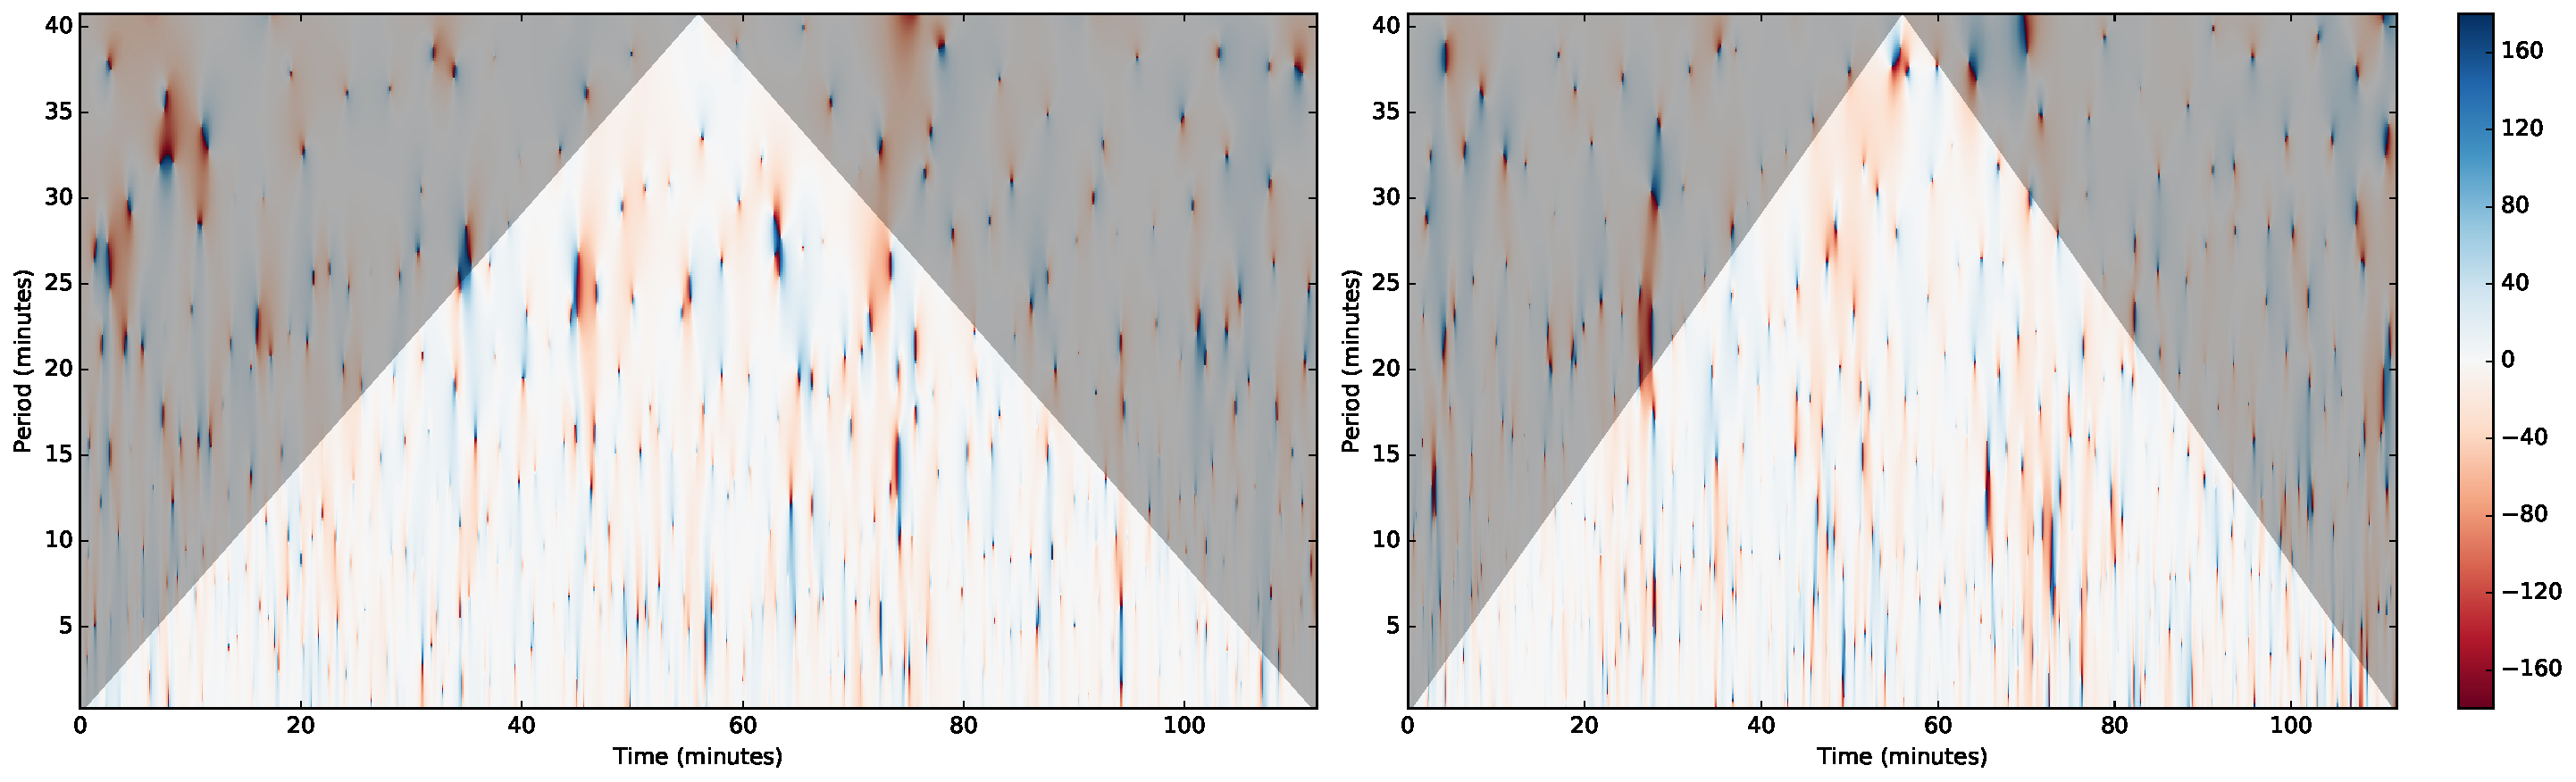
\includegraphics[width=1\textwidth]{pore_phase.pdf}
     	\caption{
	             		Same as Figure \ref{fig:phase_sunspot} but for the ROSA pore.
	             		The lowest sigma multiplier is 2 (left) and the largest is 3.5 (right).
	             		The results here show the same behaviour as the IBIS sunspot.
     		          }
     	\label{fig:phase_pore}
    \end{sidewaysfigure}
\graphicspath{{Chapter3/Figs/}}
\nobibliography*

\chapter[Analysis of Area Oscillations]{Analysis of Area Oscillations\footnote{This chapter is based on \bibentry{Dorotovic2014}. Reproduced with permission from Astronomy \& Astrophysics, © ESO}}
\label{chapter3}

   \vspace*{\fill}\par
   \pagebreak

\section{Introduction}

	Chapter 1 details the theory and thus the mechanism to observe MHD sausage modes within magnetic flux tubes. 
	The basic MHD theory has been developed since the early 1970's, as such, sunspots have been intensively studied for oscillations. 
	The commonly studied oscillatory periods in sunspots are three and five minutes.
	These oscillations are seen in intensity, line-of-sight (LOS) velocity, and LOS magnetic field.
	Moving away from LOS oscillations required more understanding of MHD wave theory in cylindrical flux tubes. 

	The MHD sausage mode are of interest here, because the sausage mode is a compressible, symmetric perturbation around the axis of a flux tube that causes density perturbations that can be identified in intensity images \citep{PMHDW}.
	Furthermore, because the wave will either compress or expand the flux tube, the magnetic field will also show signs of oscillations.
	This mode may come in two forms in terms of phase speed classification: the slow mode (often also called the longitudinal mode), which generally has a phase speed close to the characteristic tube speed and, the fast mode which has a phase speed close to the external sound speed.
	One of the main differences between the two modes is the phase relationship between appropriate MHD quantities which allows them to be differentiated.
	In this case, the fast sausage mode has an out of phase relationship between the cross-sectional area and total intensity, while the slow sausage mode has an in phase relationship.
	The technique that was applied to obtain these phase relationships are covered by, \cite{PMHDW}, \cite{Moreels2013}, and \cite{Moreels2013b}.

	Sausage modes have been observed in magnetic pores before.
	\citet{doretala2008} observed a magnetic pore for 11 hours and reported periodicities in the range of 20-70 minutes.
	These oscillations were consequently interpreted as linear low-frequency slow sausage waves.
	\citet{morton2011} used the Rapid Oscillations in the Solar Atmosphere (ROSA) instrument to also identify linear sausage oscillations in a magnetic pore.
	However, determining whether the oscillations were slow or fast proved to be difficult.

	The source and driving mechanism(s) of these MHD sausage modes have been very difficult to identify.
	Numerical simulations of a flux tube rooted in the photosphere, which is buffeted by a wide range of coherent sub-photospheric drivers, is one method for identifying the potential source of MHD sausage waves.
	These drivers can either be horizontal or vertical, single, or paired or else a power spectrum, with varying phase differences \citep[see e.g.][]{malins,khomenko,fedun2,fedun1,Vigeesh2012}.
	To understand these MHD sausage oscillations, it is necessary to firstly see if it is possible to identify the signature within solar magnetic waveguides situated in the lower solar atmosphere.
	
\section{Data collection and method of analysis}

	\begin{sidewaysfigure}
        
		\centering
		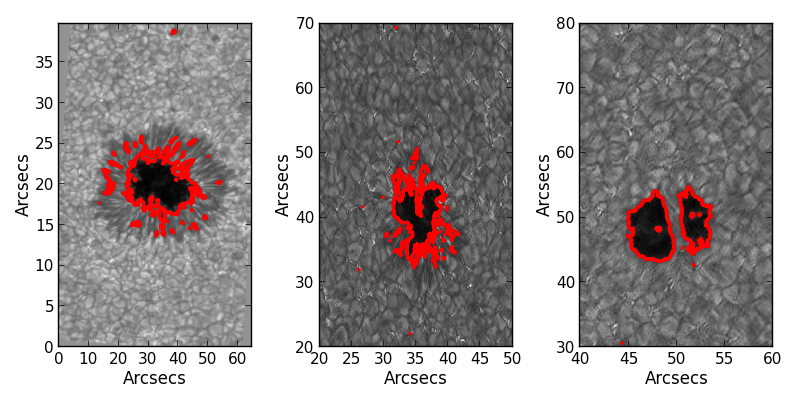
\includegraphics[width=\textwidth]{overview.png}
		\caption{
		An overview of the magnetic waveguides used for this analysis.
		\textit{(left)} The 1999 sunspot observed with the SVST with an average umbral area of 19,650 pixels (50 M km$^{2}$).
		\textit{(middle)} The 2005 sunspot observed with the DOT with an average umbral area of 12,943 pixels (32 M km$^{2}$).
		\textit{(right)} The 2008 pore observed with the DOT with an average area of 10971 pixels (27 M km $^{2}$), the light bridge that separates the pore can be seen.
		Furthermore, these structures were seen near the disk centre, so there is little to no LOS effect.
		The red line shows the thresholding technique applied to each waveguide at the start of each data series.}
		\label{images}
	\end{sidewaysfigure}

	Three time series of images with high angular resolution have been chosen here in order to demonstrate the identification of MHD sausage waves.
	The images were taken in the G-band ($430.5$ nm), which samples the low photosphere.
	This line forms deep in the photosphere and has a line intensity defined as $\rho{^2} \times$ line-of-sight column depth.
	
	The images were acquired using:

	\begin{enumerate}
		\item 
			The Swedish Vacuum Solar Telescope (SVST) situated on La Palma in the Canary Islands.
			\citet{scharmer} provides a detailed description of the features of the SVST.
			The images were taken on 7 July 1999.
			The sunspot is in Active Region (AR) NOAA 8620.
			The observing duration is 133 minutes with a cadence time of 25 seconds.
			The field of view (FOV) covers an area of $33,600$ km by $54,600$ km ($1$ pixel $\approx$ $60$ km). \citet{bonet} gives a detailed analysis of this sunspot.
			A context image is the left-handed image of Figure \ref{images}.
		\item 
			The Dutch Open Telescope (DOT) is also situated on La Palma in the Canary Islands.
			Two series of imaging data sequences were taken using this telescope.
			A detailed guide of the features of the DOT is  provided by \citet{rutten}.
			The first series of data were taken on 13 July 2005, and the sunspot is in the AR NOAA 10789.
			The region slowly decayed, and this sunspot led a small group of other magnetic structures.
			The observing length is 165 minutes and has a cadence time of $30$ seconds.
			The second set of data taken on 15 October 2008 is of a large magnetic pore with a light bridge which is about 15 pixels (750 km) wide in AR NOAA 11005.
			The duration of the observing run is 66 minutes and has a cadence time of $20$ seconds.
			Both DOT image sequences cover an area of $50,000$ km by $45,000$ km, where the maximum spatial resolution is 0.2" ($\approx$ $140$ km).
			Typical context images are the middle and right-handed panels of Figure \ref{images}.
   \end{enumerate}
   
	To obtain information relating to the cross-sectional area of these waveguides, a strict and consistent definition of the cross-sectional area is required.
	The definition is that each pixel with a value of less than $3\sigma$ of the median background intensity is counted as part of the waveguide.
	The background is defined as an area of the image where there are no magnetic features.
	This may appear to be an arbitrary definition; however, a histogram of the background intensity reveals a Gaussian distribution, and when adding the area around and including the waveguide, there is significant peak on the lower end of the Gaussian distribution curve around 3$\sigma$ or higher.
	Thus, we have a $99\%$ confidence that the area is of the structure and not of the background.
	
	Figure \ref{images} shows each waveguide at the start of the time series, where the red contour line represents the regions of cross-sectional area found.
	The definition is accurate, but, it does include some non-waveguide pixels.
	In order to reduce this factor, a bounding box is taken as close to the magnetic waveguides as possible without covering up umbral pixels.
	The total intensity was determined by summing over the intensity of each pixel found in the waveguide.
	These waveguides are not static structures as they slowly changed in size during the observing period.
	This background trend has to be removed for it not to mask any weak oscillatory signatures.
	The main reason for detrending the signal is that wavelet is computed using the Fast Fourier Transform (FFT), the signal has to have a zero mean, otherwise artefacts are introduced into the output.
	The detrending was accomplished by a non-linear regression fit and the consistency of the results was compared to subtracting the residue from an Empirical Mode Decomposition (EMD) analysis (which is explained in Chapter 2 and below).
	The residue is the data that remains after the EMD procedure has extracted as many signals as possible and it provides a very good approximation of the background trend.
 
	The resulting reduced data series were then analysed with a wavelet tool in order to extract any periods of oscillation present within these signals.
	The algorithm used is an adapted version of the IDL wavelet routine developed by \citet{torrence}.
	The standard Morlet wavelet, which is a plane sine wave with an amplitude modulated by a Gaussian function, was chosen for its suitable frequency resolution.
	The white cross-hatched area marks the cone of influence (COI), where edge effects of the wavelet structure affect the wavelet transform, and anything inside the COI is discarded.
	The white dashed line contour shows the confidence level of 95\%.
	The wavelet method is very susceptible to noise at short periods and at times may not identify the true power of short periods.
	
	Beyond this, the data representing the size and intensity has also been analysed using EMD, which decomposes the time series into a finite number of intrinsic mode functions (IMFs).
	IMFs are essentially narrowband-filtered time series, with each IMF containing one or two periods that exist in the original signal.
	The EMD technique was first proposed by \citet{huang} and offers some benefits over more traditional methods of analysis, such as wavelets or Fourier transforms (see Chapter 2).
	However, one drawback is that it is very prone to error with regards to long periods.
	The problems described above regarding the wavelet and EMD mean that the two complement each other.
	Furthermore, periods that appear in the wavelet \textit{just} below the confidence level, but appear strongly in the EMD process, is a good indication that a period is not spurious.
	At this stage, we rely on wavelet and EMD analyses, as is customary in solar physics.
	For more detail on the signal analysis, see Chapter 2.

\section{Results and discussion}

\subsection{LOS, circularity, and evolution of the waveguide}

    \begin{sidewaysfigure}
		\centering
        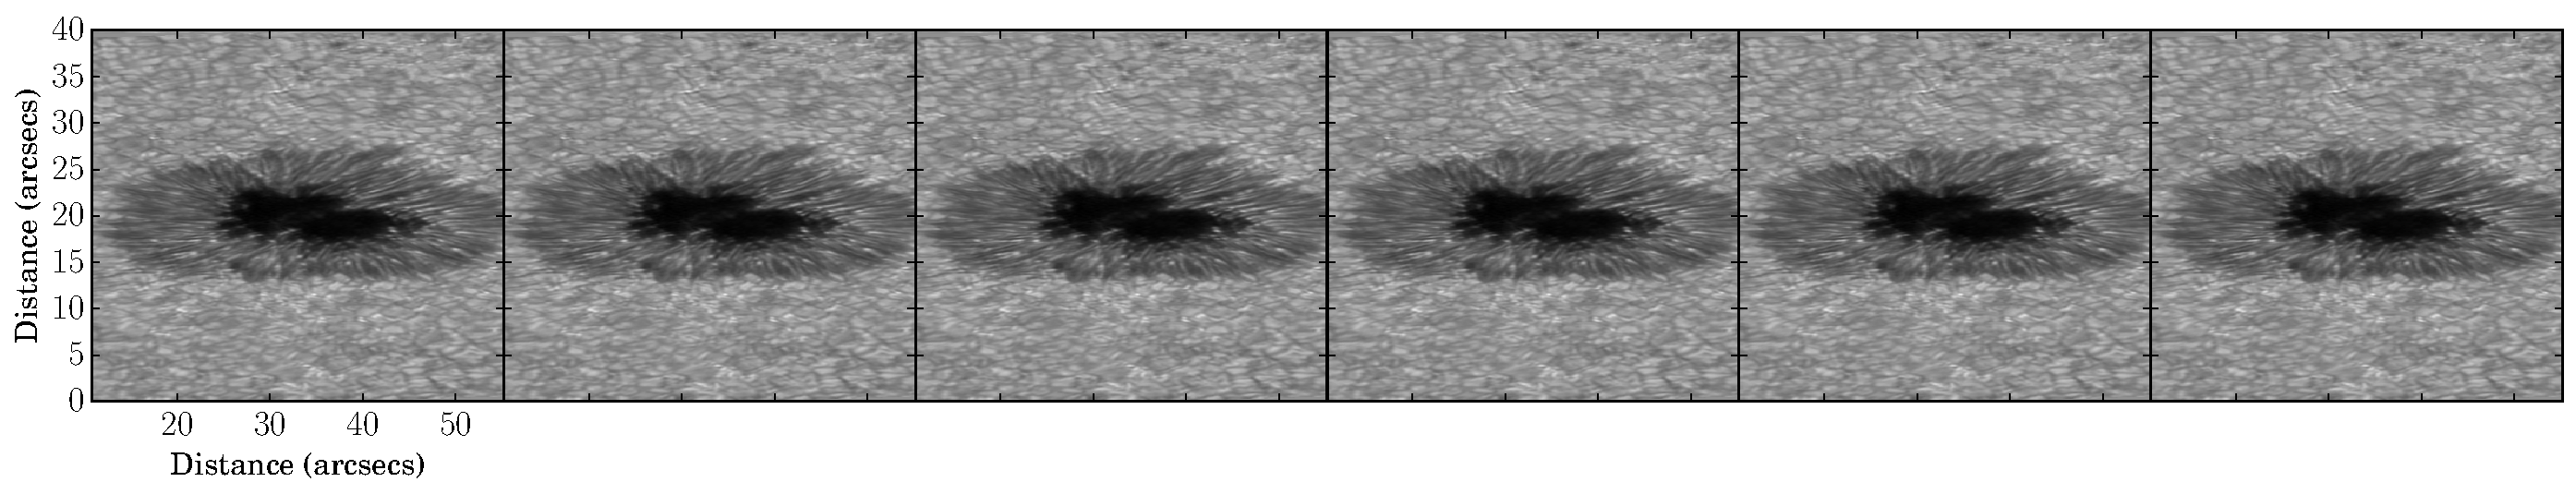
\includegraphics[height=0.19\textheight,width=\textwidth]{1999.pdf}\vspace*{-0.2cm}
        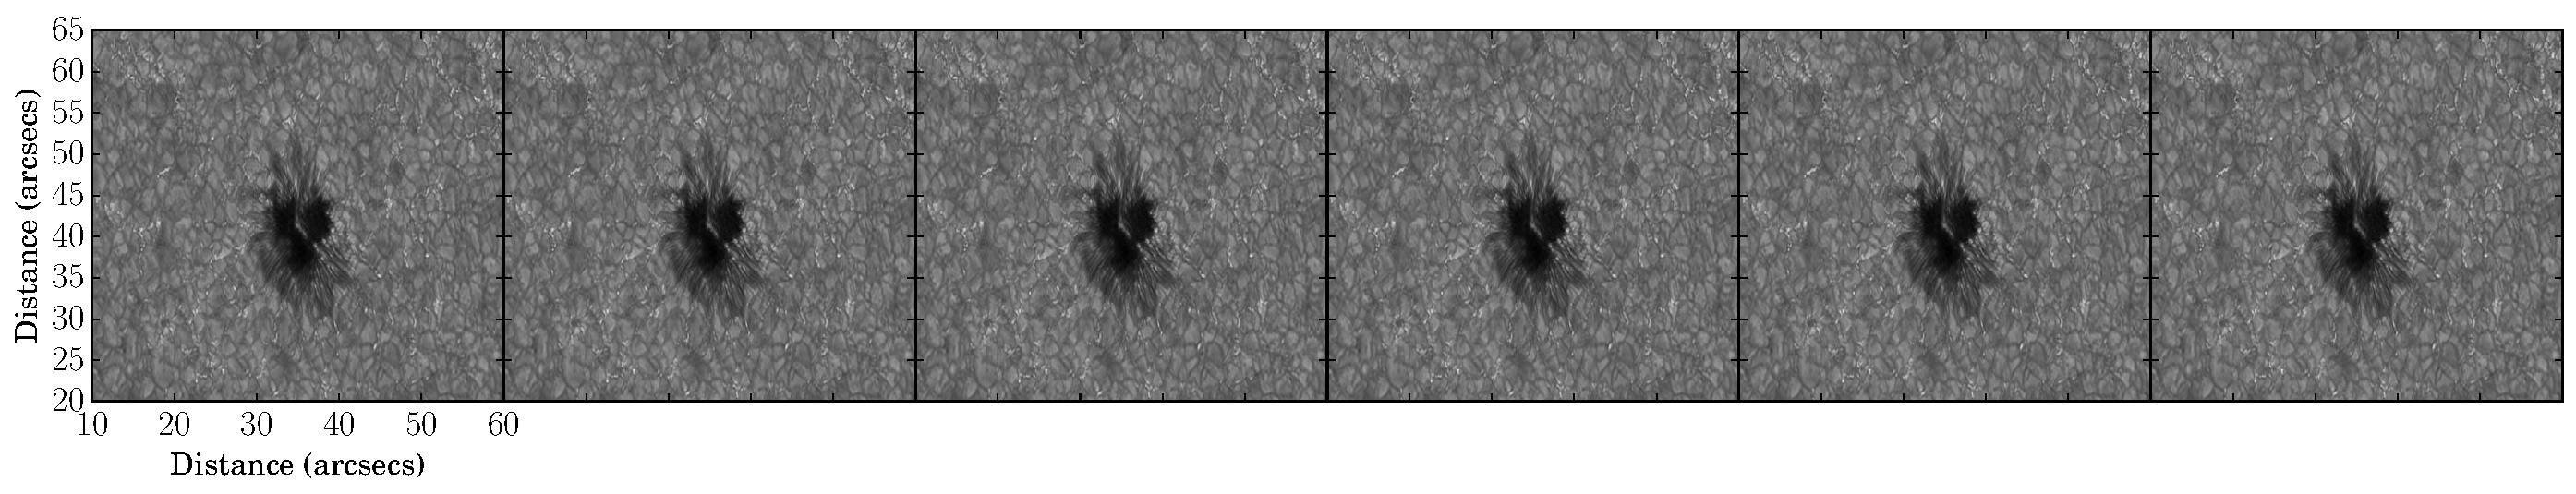
\includegraphics[height=0.19\textheight,width=\textwidth]{2005.pdf}\vspace*{-0.2cm}
        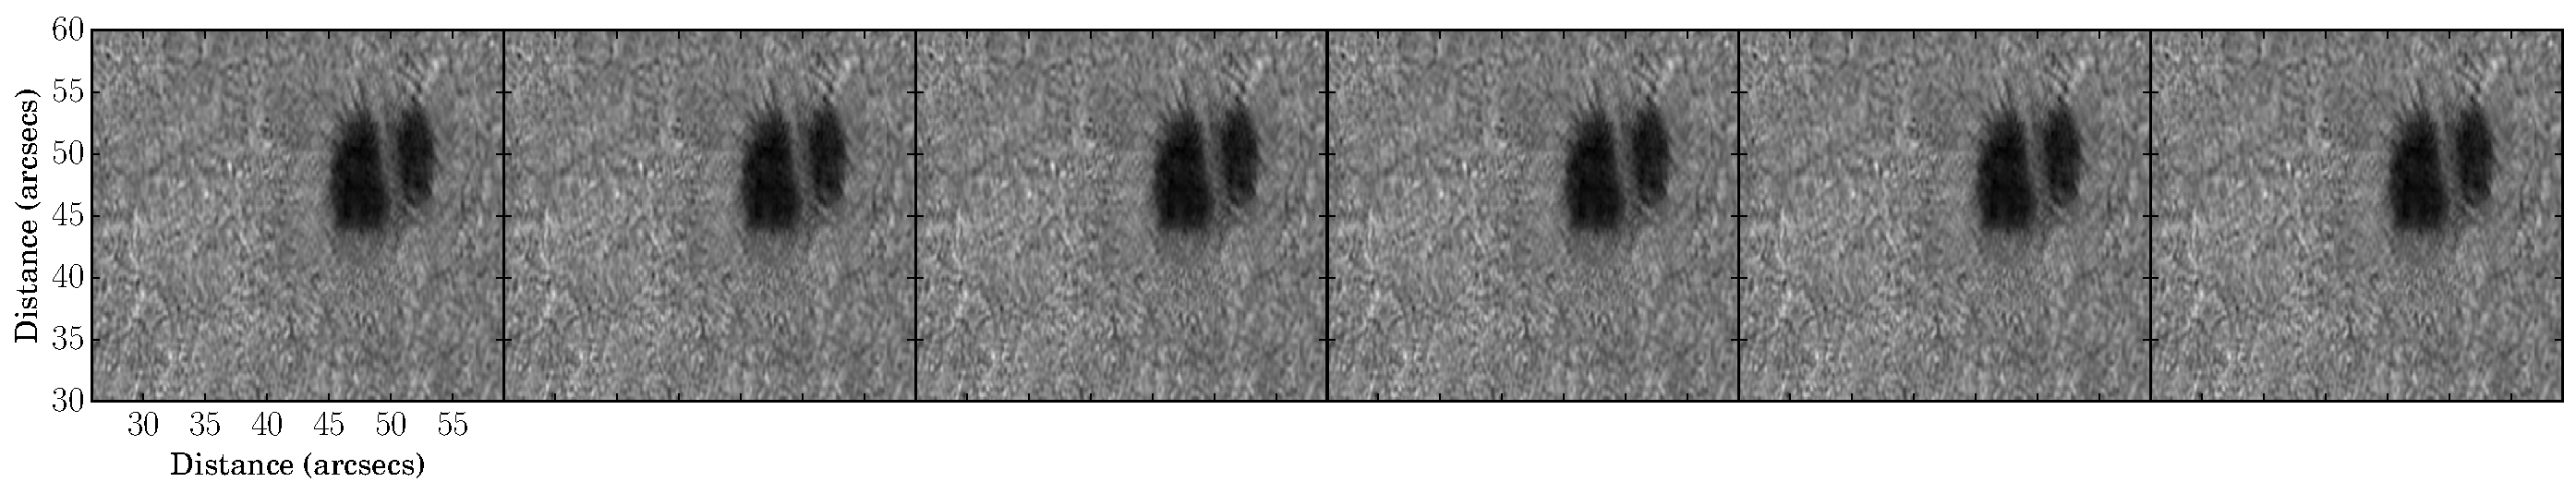
\includegraphics[height=0.19\textheight,width=\textwidth]{2008.pdf}\vspace*{-0.2cm}
        \caption{
            The three waveguides seen through six different parts of their corresponding observation sequence.
            The image sequence has time increasing from left to right.
            The first row is the 1999 sunspot, the middle row the 2005 sunspot, and the last row the 2008 pore.
                }
        \label{data}
    \end{sidewaysfigure}
	
	Several points need to be clarified for the data presented here before the full analysis.
	Firstly, there are LOS issues, \citet{2003A&A...397..765C,2003A&A...409..325C} have investigated how the LOS angle affects various aspects of observing coronal loops in a 2D model.
	Overall they found that for the slow sausage MHD wave, for a range of angles from $\pi/6$ to $\pi/3$, the observed intensity decreases as the LOS angle increases.
	Secondly, the larger angles lengthened the \textit{observed period} of the wave.
	While the objects here are not coronal loops, the LOS angle still matters and should behave similarly.
	The LOS angles in all three cases were less than 30$^\circ$ thereby limiting any relevant effects of LOS.
	
	Sunspots or magnetic pores are not fully circular and can have arbitrary shapes.
	The effects of a non-circular shape have been studied by, for example, \citet{2003A&A...409..287R}, \citet{2009A&A...502..315M}, and \citet{2011A&A...527A..53M}.
	While they do not account for the very complicated and real structure of the sunspots and magnetic pores observed here, they still offer an adequate insight.
	Current theory suggests the shape will have a minor effect on the oscillations unless it has a significant deviation from circularity.
	Likewise, the structure of each waveguide undergoes a minor change during the observation campaign, limiting any effects from large-scale structural change, as can be seen in Figure \ref{data}.

\subsection{MHD theory for phase relations}
	
	Treatment of the MHD equations makes it possible to determine phase relations between various physical quantities for propagating and standing MHD waves.
	This has been summarised briefly by \citet{goedbloed} and also applied by \citet{PMHDW}.
	The latter find that the phase relation for the slow MHD wave with regards to cross-sectional area and density is in phase regardless of whether the wave is propagating or standing.
	More recently, \citet{Moreels2013} have expanded on this idea, taking factors into account such as LOS, which were neglected earlier, but also expanding the theory to cover fast MHD sausage waves.
	The phase relation for the magnetic field to the cross-sectional area is in phase when assuming that the magnetic field is frozen into the plasma.
	
	Supplementary information from other perturbation phase relations, such as the LOS velocity and the LOS magnetic field, allows one to determine whether the observed MHD wave is slow or fast.
	In summary, the slow MHD sausage mode shows in phase behaviour between intensity and area perturbations, while the fast sausage mode shows out of phase behaviour.
	Before progressing, we need to address the opacity effect on MHD wave perturbations.
	This is relevant, since intensity fluctuations can be due to the change of the optical depth along the LOS, which has the same phase difference as the fast MHD sausage wave and as a result is indistinguishable without further information \citep{PMHDW}.
	
	Recently, \citet{Moreels2013b} have analytically determined the phase difference between the cross-sectional area and the total intensity perturbations for both the slow and fast MHD sausage modes.
	Note that any mention of the area means the cross-sectional area from here on in and the intensity means the total intensity.
	They find that, for both the slow body and surface MHD wave, the behaviour is in phase, while for the fast surface wave, the behaviour is out of phase.
	This result means that it is possible to approximately separate slow and fast sausage waves without the use of other observable variables. Their results will be used here to distinguish between slow and fast MHD sausage modes.

\subsection{Sunspot, 7 July 1999 , AR 8620}

   \begin{sidewaysfigure}
	   \centering
       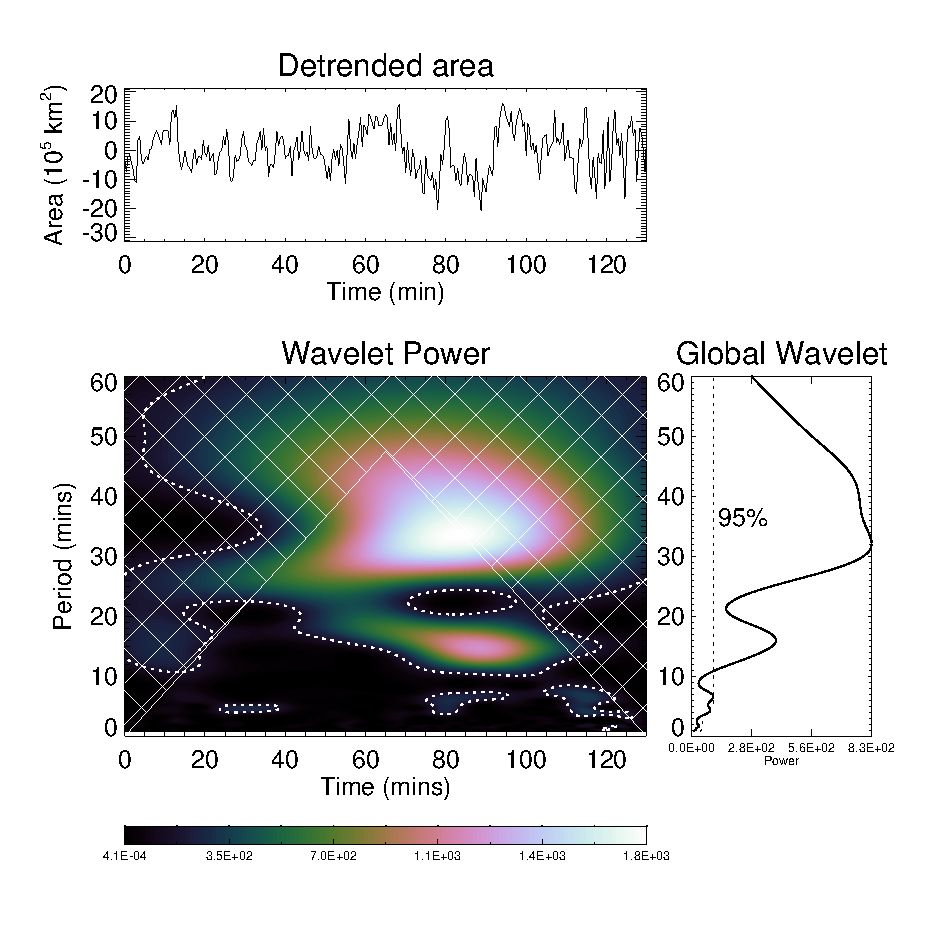
\includegraphics[width=0.49\textwidth]{1999_wl.eps}
       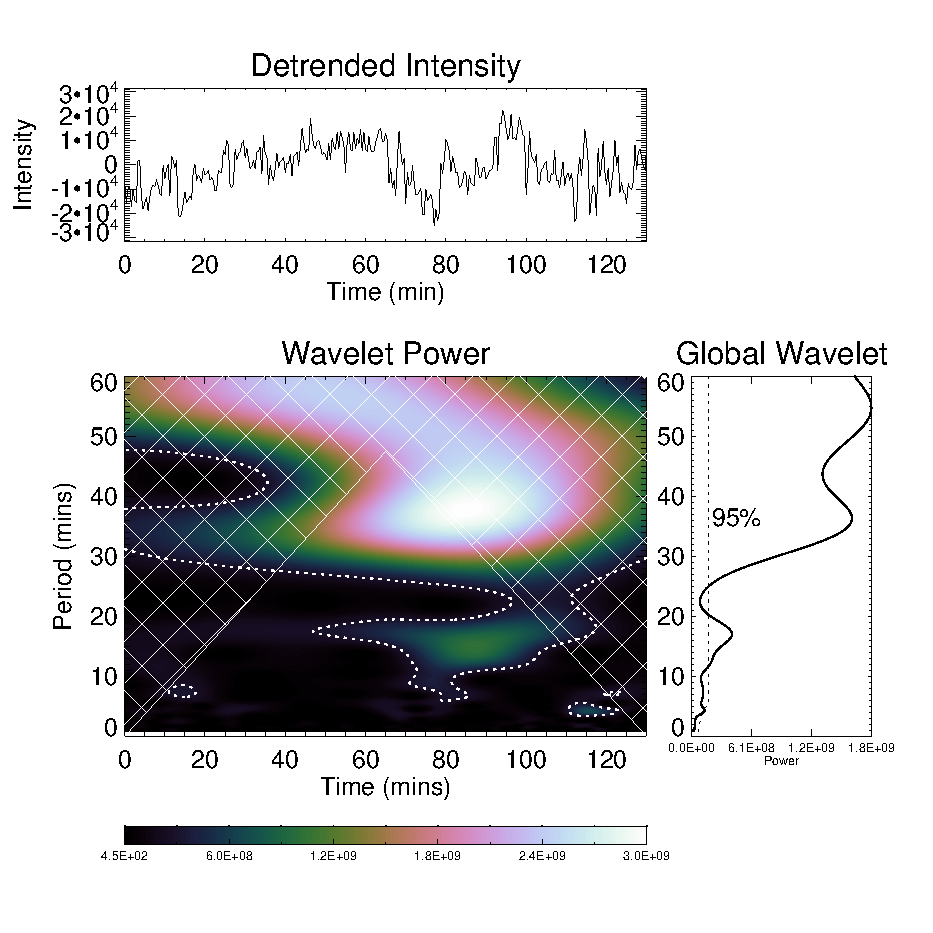
\includegraphics[width=0.49\textwidth]{1999_wl_inten.eps}
	   \caption{
				\textit{(left image)} Evolution of the area of the 1999 sunspot.
				\textit{(right image)} The same as the left image but for the total intensity of the 1999 sunspot.
				\textit{(upper panel)} The signal that is analysed.
				\textit{(lower panel)} The wavelet power spectrum for a white noise background, the cone of influence is marked as a cross-hatched area where edge effects become important and the contour lines show the 95\% confidence level.
				\textit{(lower right panel)} Global (integrated in time) wavelet power spectrum, where the dashed line shows the 95\% confidence limit.   
				}
	   \label{1999sunspot}
   \end{sidewaysfigure}
   	
	Figure \ref{1999sunspot} shows the wavelet analysis of the 1999 sunspot's area and intensity data. There are four confidently identified periods that exist in the area wavelet with 95\% certainty; 4, 7, 16, and 32 minutes.
	The 32-minute period is found over a wide range of the time series, with some of its power inside the COI.
	However, most is outside the COI.
	The 16-minute period is strongly localised at 50 to 120 minutes of the data series, starts at 18 minutes, and slowly increases and stabilises at 14 minutes.
	There is a third and fourth period at four and  seven minutes that just reach the significance level and appear sporadically during the time series.
	
	The intensity wavelet shows three distinct periods of oscillations above the confidence level: 4, 16, and 36.5 minutes.
	The 36.5-minute period has a corresponding area wavelet oscillation at 32 minutes.
	While the 16-minute oscillation corresponds to the 16-minute oscillation found in the area.
	Furthermore, the 16-minute period starts with very concentrated power and does not display the same period change as the area oscillation does.
	Finally, the four-minute period also corresponds to an oscillation found in the area but is also sporadic in its appearance.
	
	It is safe to say that these oscillations are caused by sausage waves.
	The reason is that in linear ideal MHD theory, the sausage wave is the only MHD wave capable of changing the area of the flux tube that is observed on disk \citep[see e.g.][]{2003A&A...397..765C,CLOO}.
	Without the ability to directly compare the phase difference of the area to the intensity, great caution needs to be exercised to determine with confidence whether the perturbations are fast or slow.
	A wavelet phase diagram reveals regions (where the wavelet coherence is high and the period is $\le 20$ minutes) to be either out of phase or in phase, but a clear image of constant phase difference does not appear.
	This might be due to mode conversion occurring in the sunspot, since the G-band samples a region where the plasma-$\beta$ $\approx 1$ in a magnetic structure \citep{gary}.
	When the period is $\ge 20$ minutes, the only area of high coherence is located around 30 minutes and found to be nearly out of phase, which hints that there might be a fast surface sausage wave.
	However, only two full wave periods are outside the COI, which is due to the total length of the data series.
	This behaviour indicates that for short periods, a mixture of fast surface and slow MHD sausage waves are present while for the long period, it is purely a fast surface MHD sausage wave.
		
	
	\begin{sidewaysfigure}
	\centering
	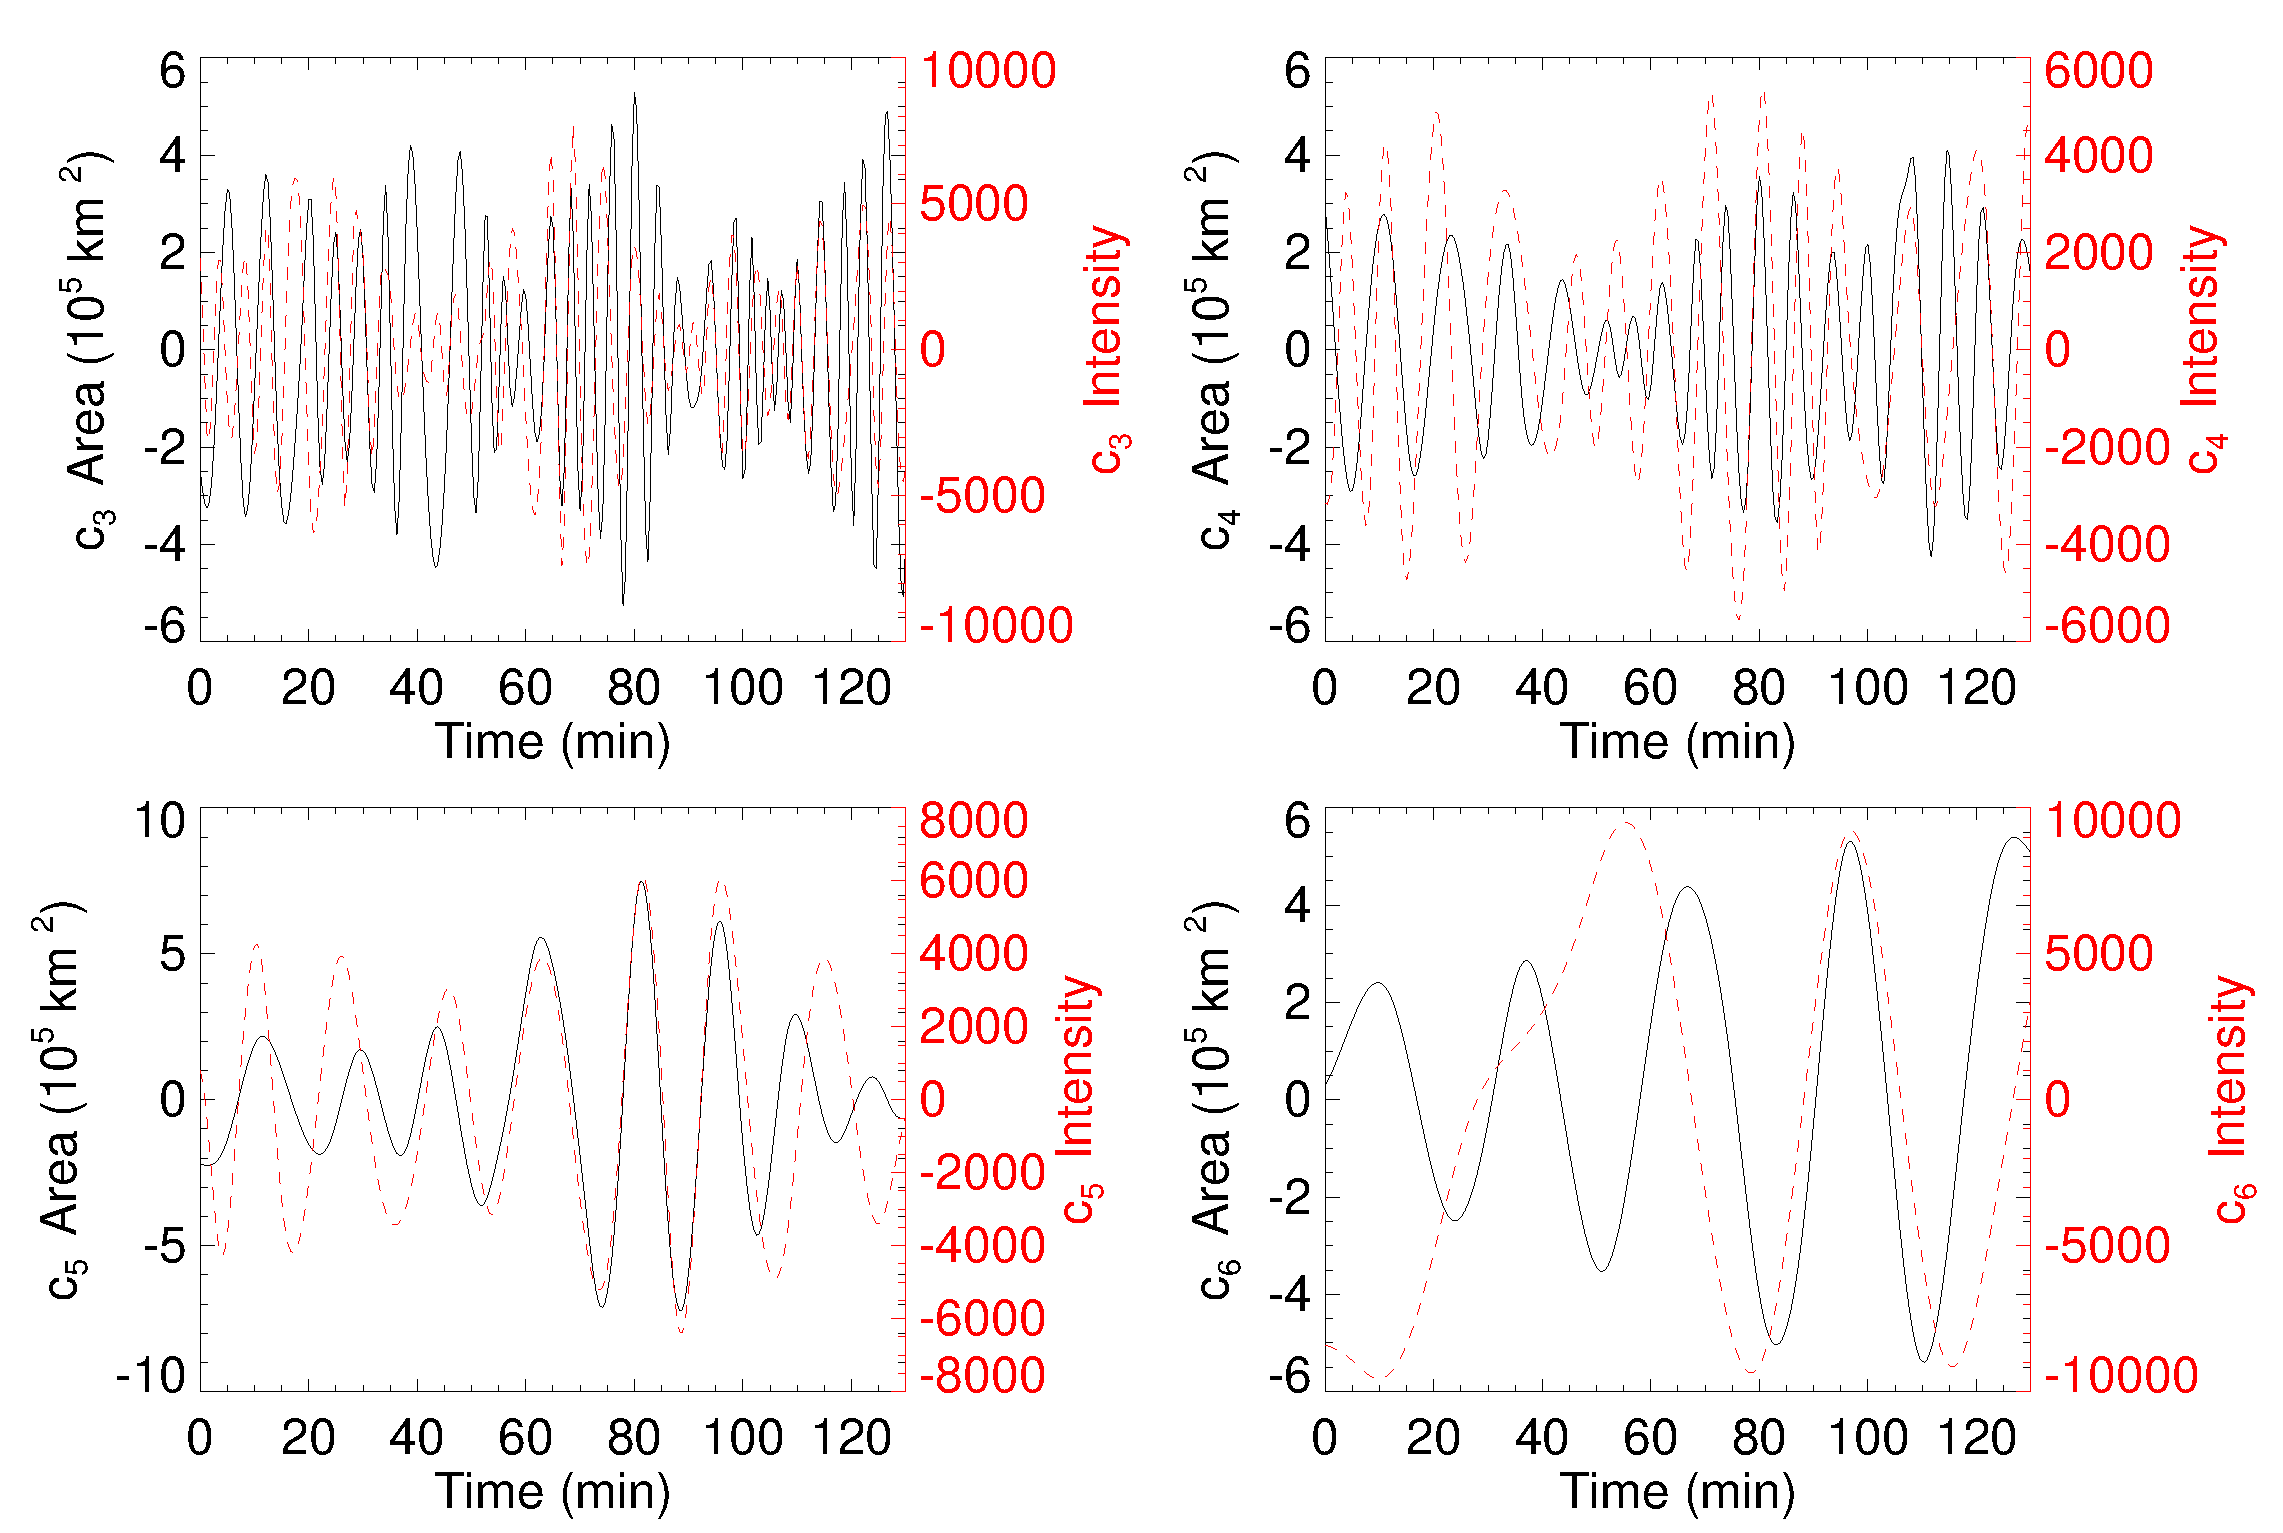
\includegraphics[width=\textwidth]{1999_IMFs.eps}
    \caption{
	      	The IMFs of the evolution of the area (red) and intensity (black) for the 1999 sunspot, over-plotted to aid comparison.
	      	Generally after the $6$th IMF, higher IMFs lack a sufficient number of wave periods, which makes it difficult and less reliable to obtain an accurate period.
   		    }
    \label{1999IMF}
	\end{sidewaysfigure}
		
	Figure \ref{1999IMF} shows the computed IMFs for the 1999 sunspot data set.
	The IMFs show the periods of oscillations identified using the EMD algorithm.
	IMFs which show irrelevant periods, or the residual signal which are ignored.
	In general, the higher order IMFs tend to show longer periods and, as such, contain fewer wave periods, which makes phase identification less reliable.
	Four IMF overlays are shown, and IMFs with similar periods to the wavelet plots have been overlaid in order to aid comparison for each dataset.
	
	Four IMFs directly coincide with the wavelet period that reveal both area and intensity perturbations.
	IMF $c_{3}$ displays the four-minute period where major regions of in phase behaviour can be seen; however, both side shows one or two wave periods of out of phase behaviour.
	IMF $c_{4}$ exhibits a period of seven minutes.
	The picture here is more muddled as an extra period is present in the intensity, namely 11 minutes, making phase identification harder for the seven-minute period.
	Where the IMFs coincide with the same period, namely at the start of the time series, the phase difference is approximately 45 degrees, which the author have no theoretical explanation for.
	IMF $c_{5}$ displays a 16-minute period, with in phase behaviour.
	Finally, IMF $c_{6}$ contains the 32-minute period.
	This period does not fully match the period seen in the intensity, but also one of the edge effects of the EMD process can be seen in the intensity signal.
	Near the end of the time series, the two IMFs overlap with the same period with an in phase behaviour.
	In summary, the EMD process shows that the major behaviour is in phase, indicating the existence of a slow sausage mode.
	Also the regions of changing phase difference at lower periods indicates the potential existence of a fast surface mode as the phase difference matches.
	The reason for the wave being restricted as only a surface mode is due to current theory that suggests that the fast body mode is not supported in photospheric flux tubes \citep{Moreels2013,Moreels2013b}. 
	However, the last IMF does not agree with the wavelet phase due to the artefact from the EMD process.
	
	It was possible to approximately separate the penumbra from the umbra and investigate its area for oscillations.
	However, the penumbra is a highly dynamic object and this makes the area estimation reasonably uncertain.
	There seem to be four periods that exist at 95 \% certainty: 5, 9, 15, and 25.
	The three shorter periods (5, 9, and 15 minutes) closely correspond to the 4, 7, and 16-minute oscillations in the umbra; they could be a continuation of these umbral periods that became up-shifted as they enter the less compact structure of the penumbra.
	While the 25-minute period does not directly correspond to an observed area oscillation.
	The wavelet phase analysis shows large regions of out of phase behaviour where the period is either below ten minutes or above 20 minutes.
	This behaviour is a mixed collection of fast surface and slow sausage modes, with regions moving from one phase difference to another after three or more wave periods.

\subsection{Sunspot, 13 July 2005, AR 10789}
   
   \begin{sidewaysfigure}
   \centering
   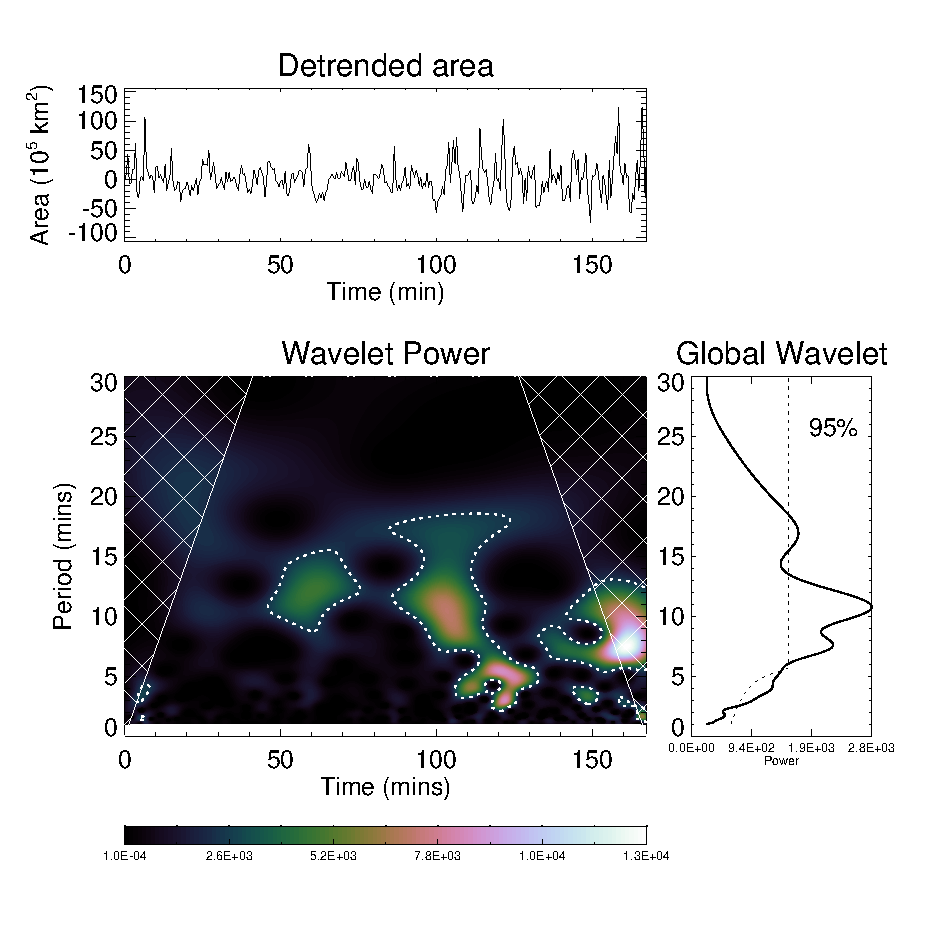
\includegraphics[width=0.49\textwidth]{2005_wl.eps}
   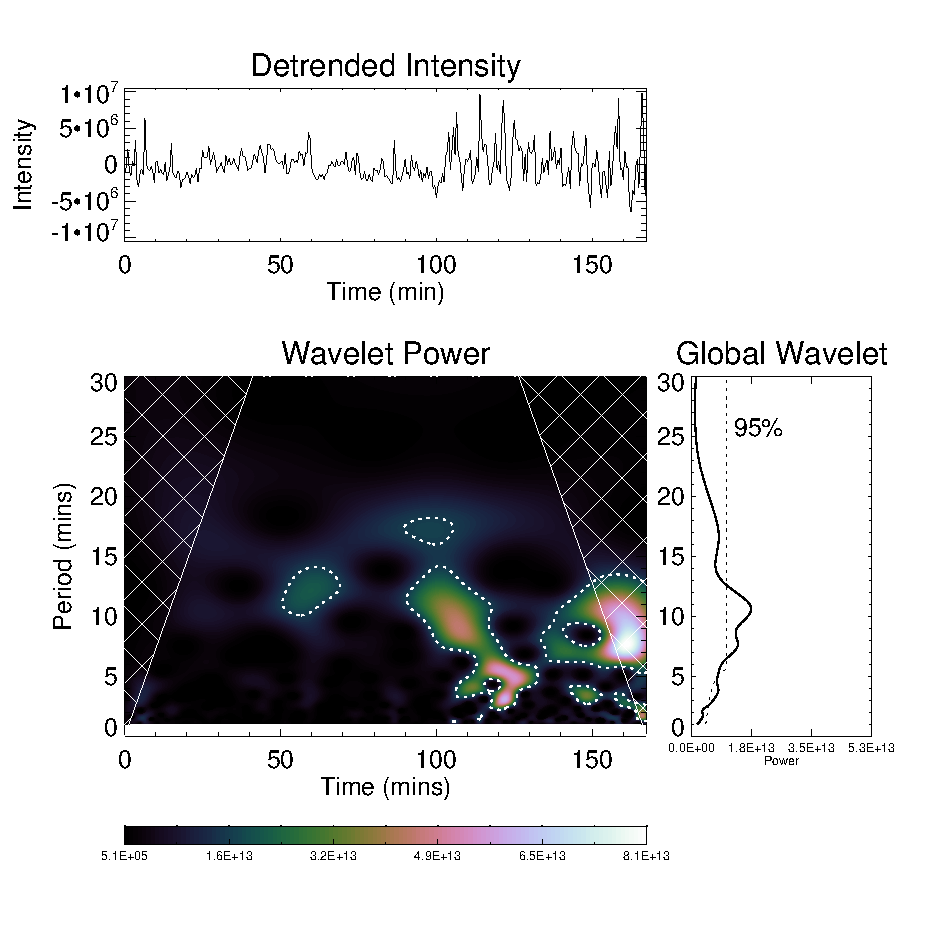
\includegraphics[width=0.49\textwidth]{2005_wl_inten.eps}
      \caption{
      			Same as Figure \ref{1999sunspot} but for the sunspot in AR 10789 observed in 2005.
      		  }
      \label{2005sunspot}
   \end{sidewaysfigure}

   \begin{sidewaysfigure}
   \centering
   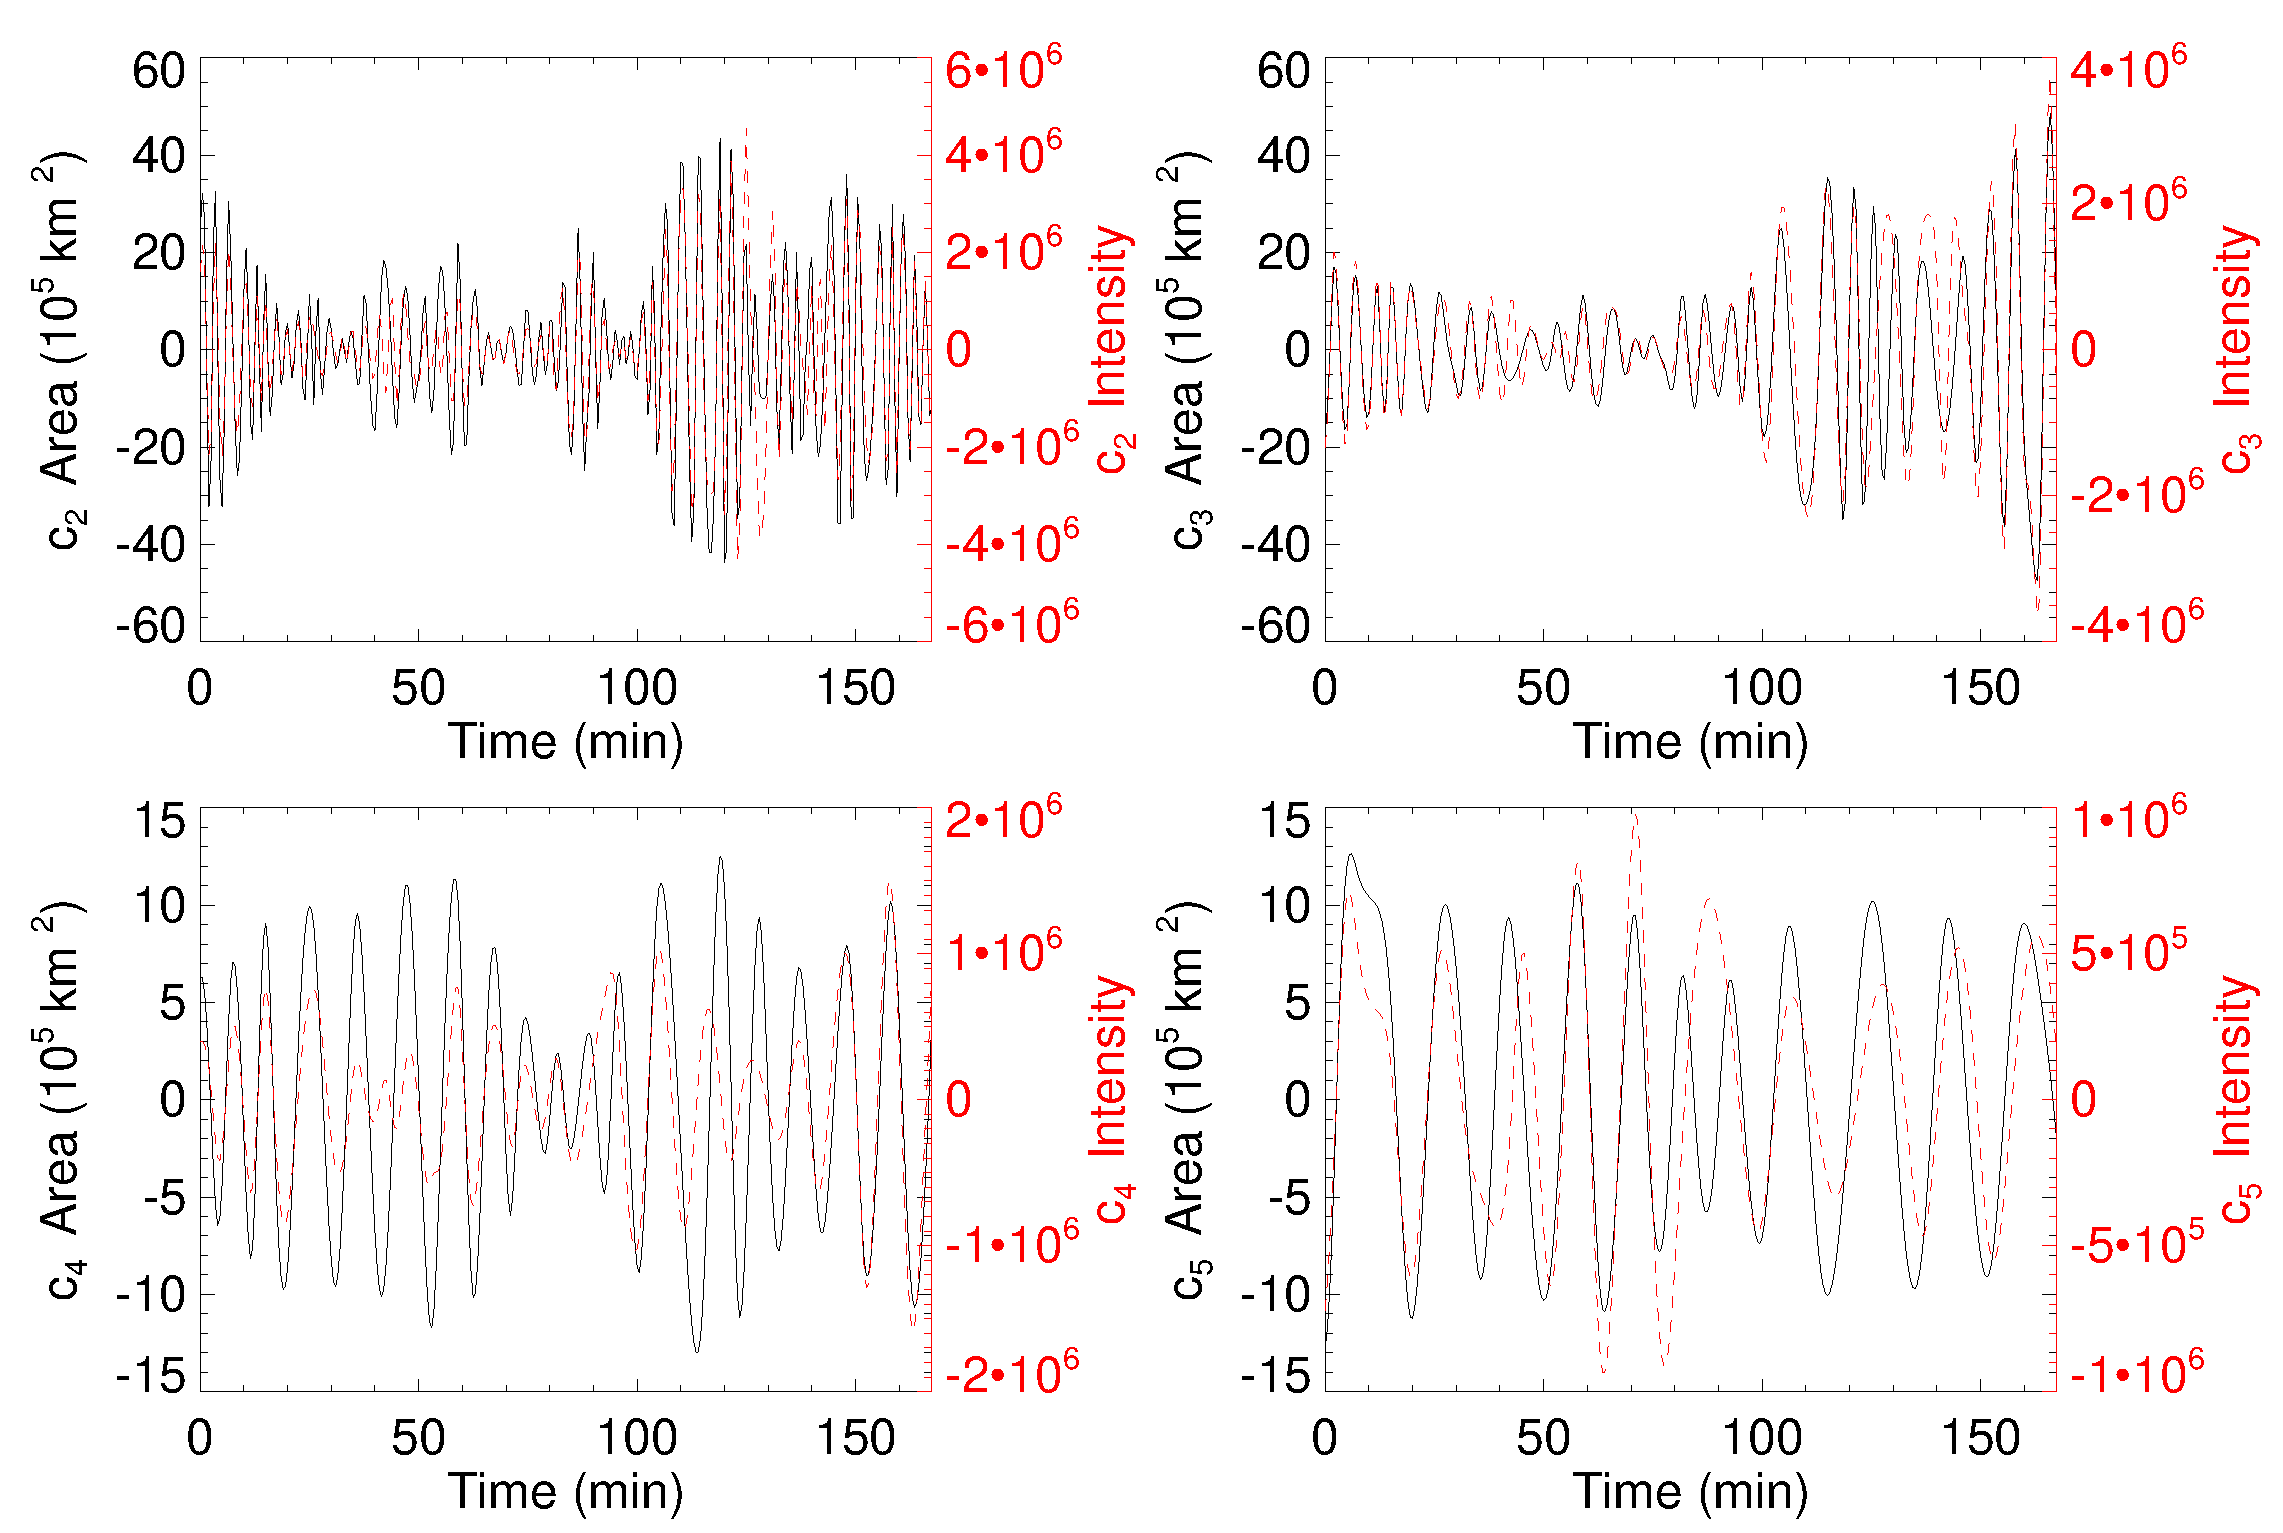
\includegraphics[width=\textwidth]{2005_IMFs.eps}
      \caption{
      			Same as Figure \ref{1999IMF} but for the sunspot in AR 10789 observed in 2005.
      		  }
      \label{20005IMF}
   \end{sidewaysfigure}
   
	Figure \ref{2005sunspot} shows the wavelet analysis of the 2005 sunspot area and intensity in AR 10789.
	There are four periods that exist at 95\% confidence level: 4, 7.5, 11, and 16.5 minutes.
	Each period has a region of high power in the wavelet, with the lower periods appearing nearer the end of the time series.
	The corresponding intensity wavelet reveals that there are three periods of 4, 7.5, and 10.5 minute oscillations; however, the 16.5-minute oscillation is present but is a very weak signal.
	The cross-wavelet phase indicates that these oscillations are in phase.
	There are no major regions of out of phase behaviour.
		
	Figure \ref{20005IMF} shows the IMFs for the area and the intensity of the sunspot data in AR 10789.
	In this case, each period is found by the EMD process. IMF $c_{2}$, IMF $c_{3}$, IMF $c_{4}$, and IMF $c_{5}$ correspond to the 4, 7.5, 11, and 16.5-minute oscillation periods, respectively.
	IMF $c_{2}$ displays extensive in phase behaviour throughout the time series, which is a strong indication of the slow sausage MHD wave at a period not too dissimilar to the global \textit{p}-mode oscillation.
	The region of interest is within the time interval of 90 to 130 minutes for IMF $c_{4}$, where the wavelet has these oscillations.
	The IMF shows clear in phase behaviour in this time interval.
	The overall phase relation between the area and intensity indicates the presence of slow sausage waves.
	
\subsection{Magnetic pore, 15 October 2008}

   \begin{sidewaysfigure}
   \centering
   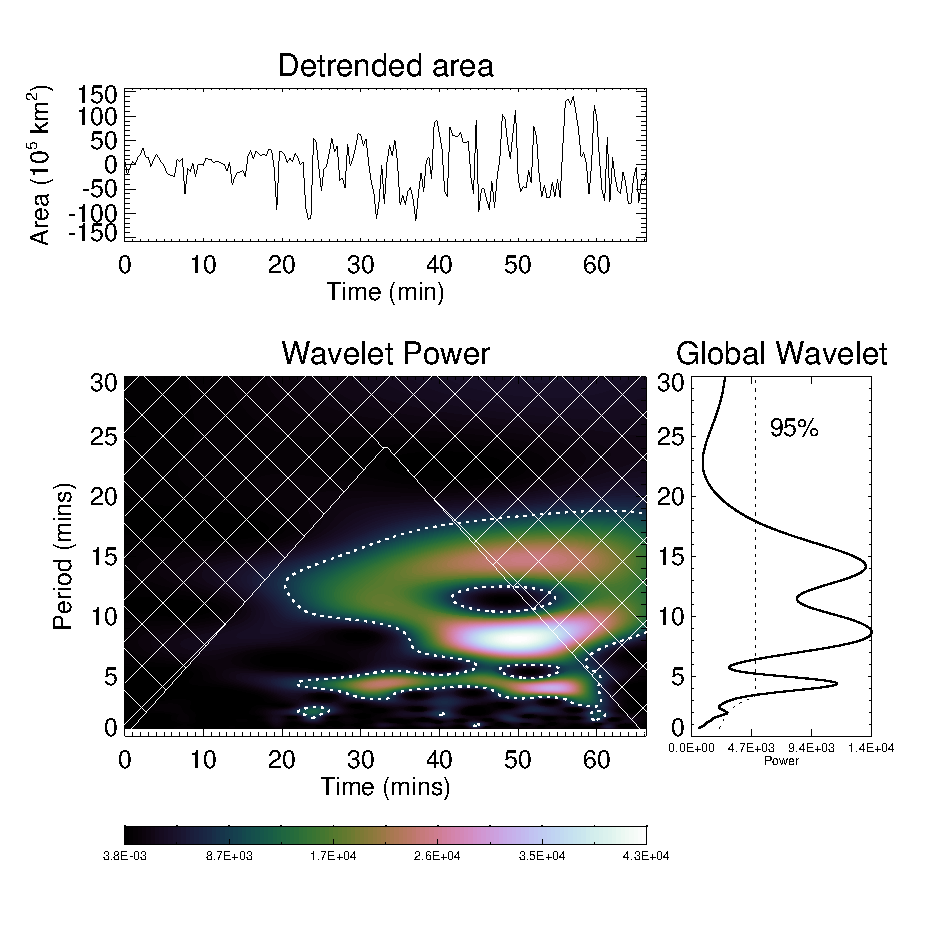
\includegraphics[width=0.49\textwidth]{2008_wl.eps}
   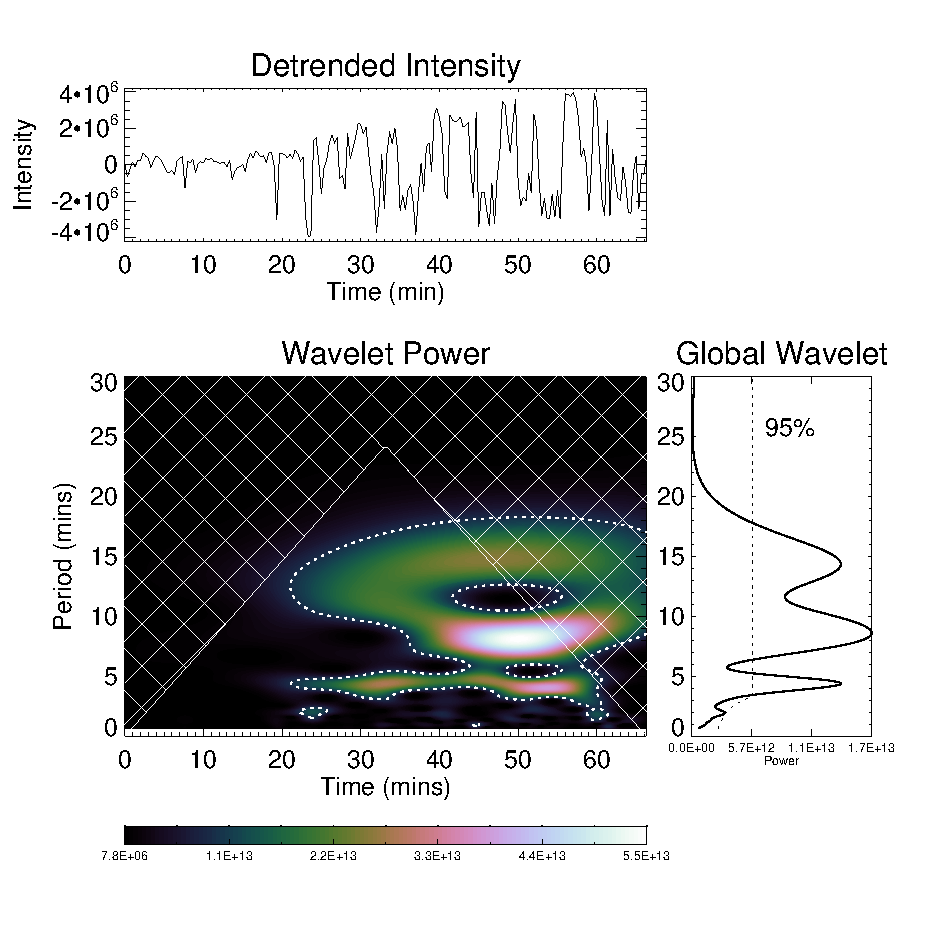
\includegraphics[width=0.49\textwidth]{2008_wl_inten.eps}
   	   \caption{
      			Same as Figure \ref{1999sunspot} but for the magnetic pore in AR 11005 observed in 2008.
 		      }
      \label{2008pore}
   \end{sidewaysfigure}
   
     \begin{sidewaysfigure}
     \centering
     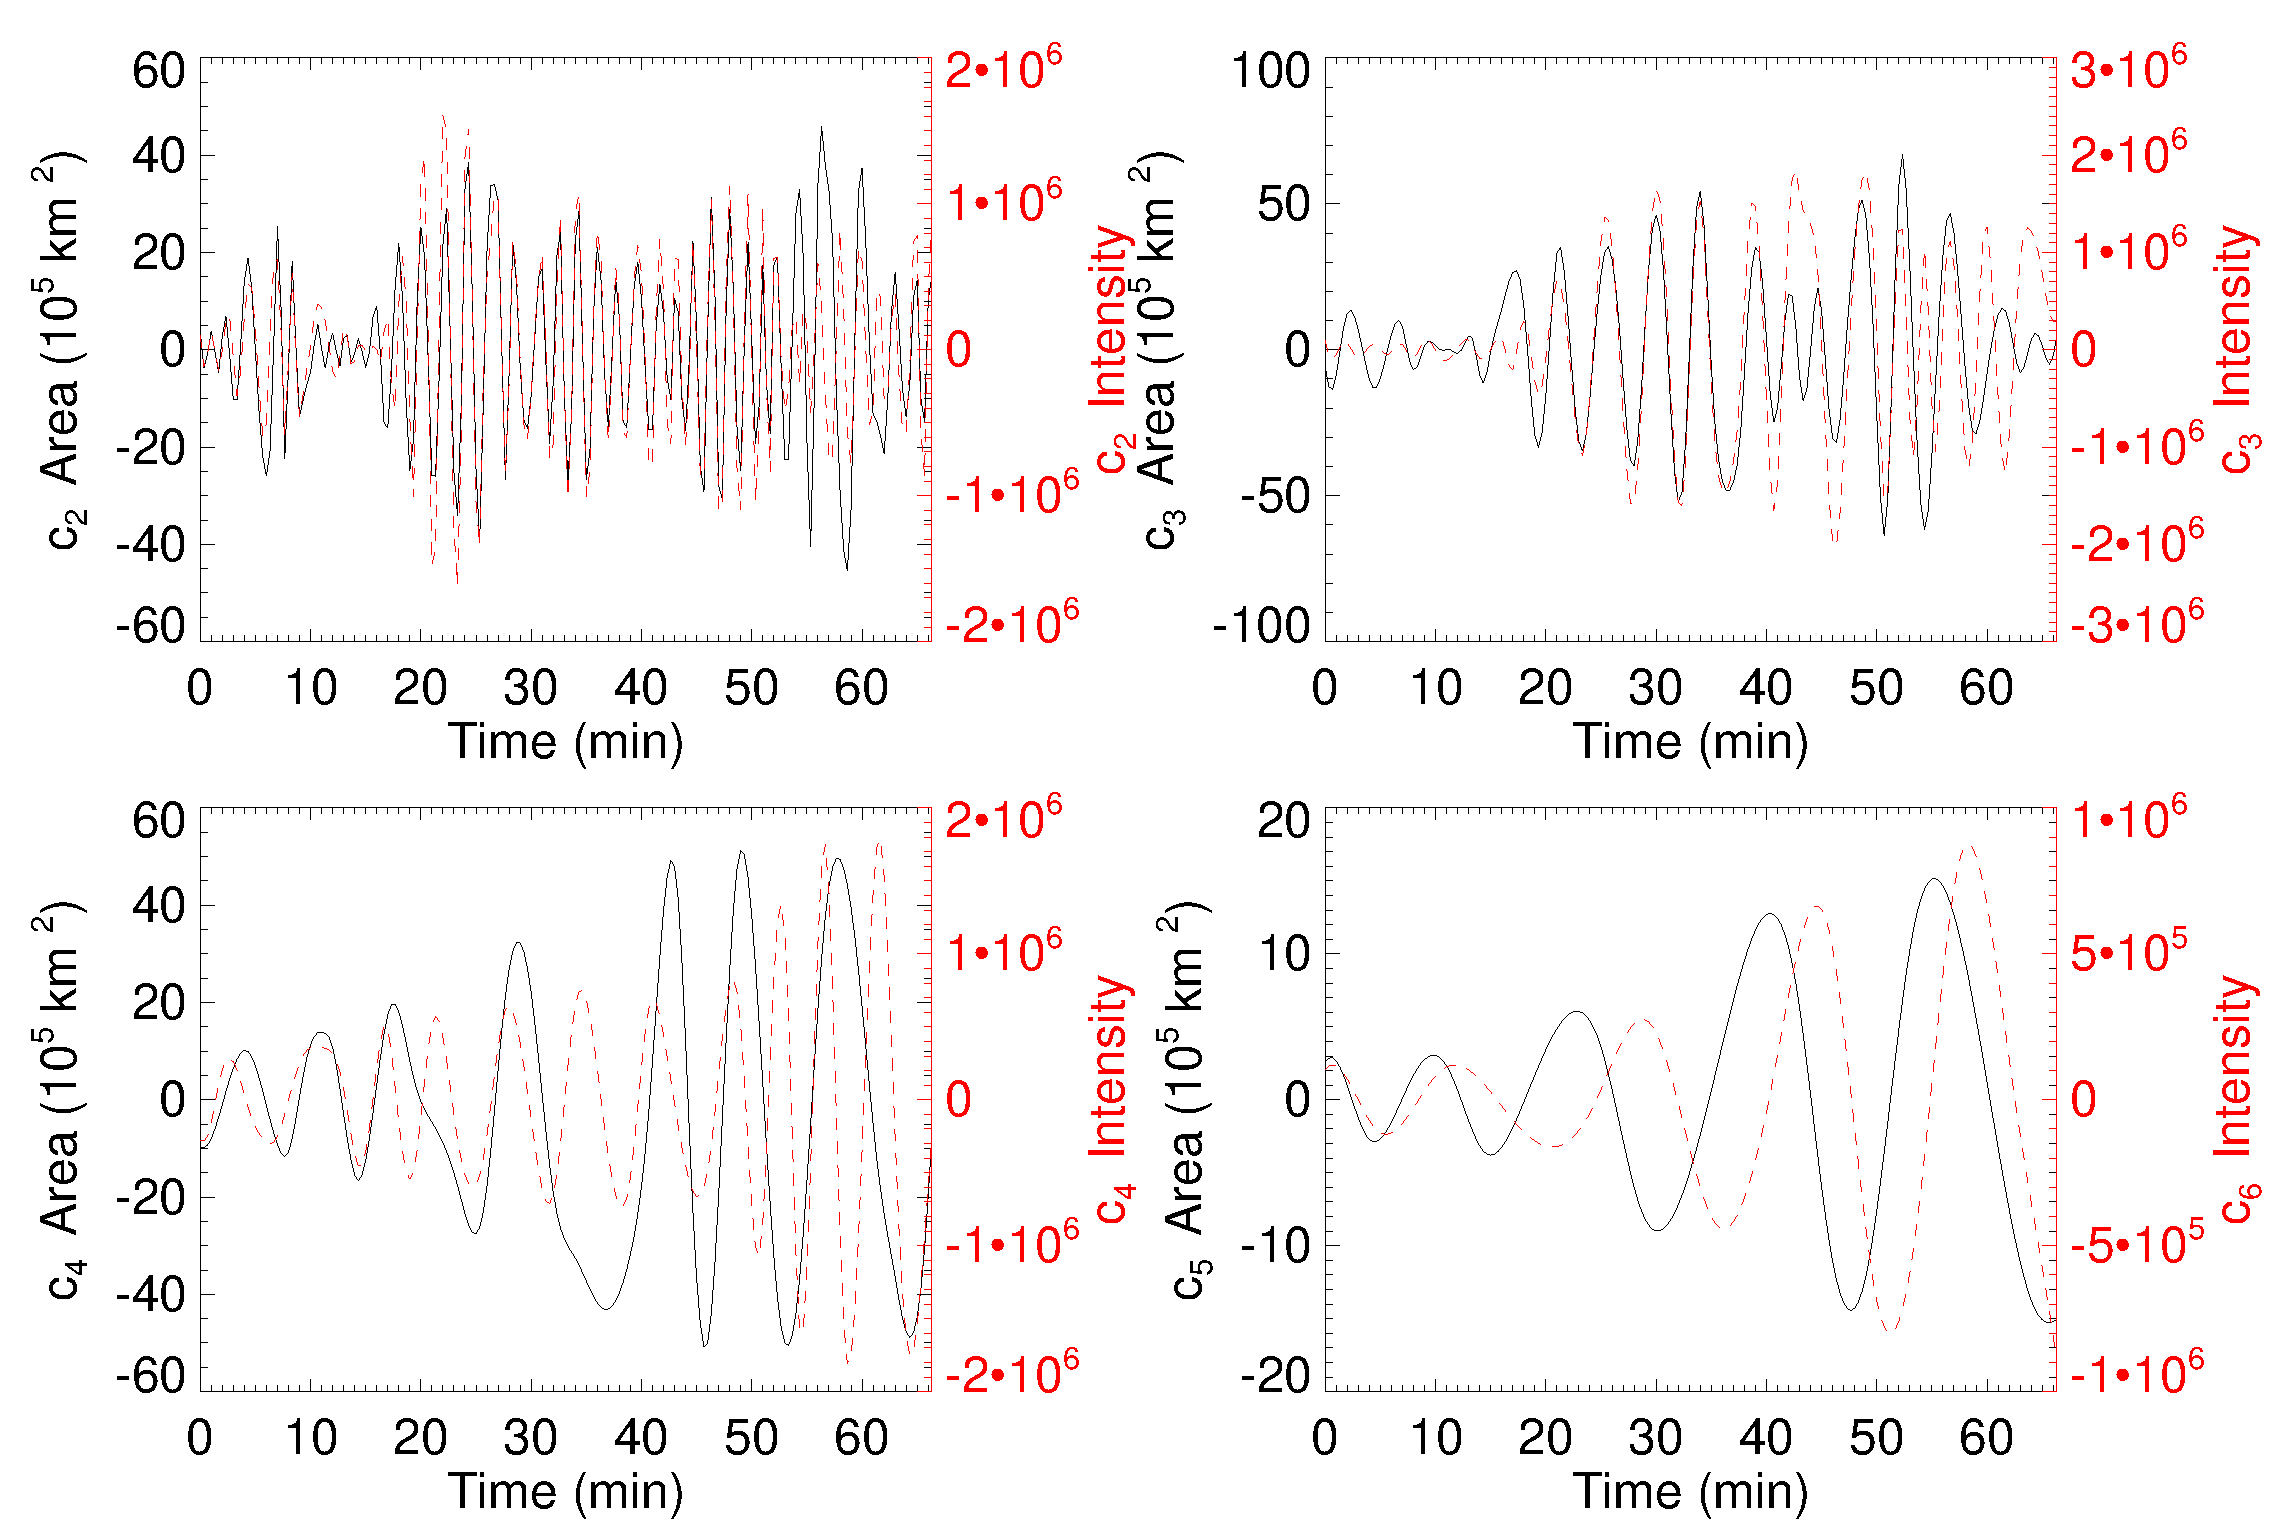
\includegraphics[width=\textwidth]{2008_IMFs.eps}
     \caption{
       			Same as Figure \ref{1999IMF} but for the magnetic pore in AR 11005 observed in 2008.
        		  }
     \label{20008IMF}
     \end{sidewaysfigure}
      
	Figure \ref{2008pore} shows the wavelet analysis of the magnetic pore with a light bridge.
	There are three periods that exist at 95 \% confidence level: 4.5, 8.5, and 14.5 minutes.
	The large part of the power of the period of 14-15 minutes is inside the COI; however, the period appears in the EMD analysis and has a large portion of power outside the COI and thus has not been ignored for this analysis.
	The three periods are seen in both area and intensity data when the wavelet analyses are cross-correlated.
	The power for these two periods is concentrated in the time interval of 20 to 60 minutes.
	The cross-wavelet analysis shows that the overlapping time span is somewhat smaller, at about 30 to 50 minutes.
	Furthermore, the wavelet power for each period runs parallel to each other throughout the time series, and they appear at the same time and seem to fade away at a similar time as well.
	
	Figure \ref{20008IMF} shows the IMFs for the area with intensity over-plotted.
	In this case, IMF $c_{3}$ indicates a period of 4.5 minutes and IMF $c_{4}$ has a characteristic period of 8.5 minutes, and this applies to both the area and intensity IMFs.
	IMF $c_{3}$ reveals that the phase relation is in phase for the majority of the time series.
	IMF $c_{4}$ reveals large regions of roughly in phase behaviour but with, again, a 45-degree phase difference.
	Not shown is the comparison of IMF $c_{4}$ and IMF $c_{5}$ for the area and intensity, respectively.
	At the end of the time series for both, there is a mixture of in phase behaviour but also with the intensity signal leading the area signal for the 8.5 minute oscillation.
	IMF $c_{5}$ and IMF $c_{6}$ for the area and intensity, respectively, show a period of 14.5 minutes.
	There is a region of near out of phase behaviour before this then turns into 45-degree phase difference with the area leading the intensity perturbations.
	Consistently, there are occurrences of unexplainable phase differences that require new MHD theory in order to explain.
       
	The easiest way to confirm the linearity of waves is to compare the amplitude of the oscillations to the characteristic scale of the structure.
	In all three cases studied here, the oscillation amplitudes are around 10\% or less of the total area, which indicates that these oscillations are linear.
	Furthermore, the amplitude of the oscillation in the last two cases is by and large the same, so the amplitude has scaled with the size of the structure.
	However, for the 1999 sunspot, the amplitude of the oscillation is an order of a magnitude less. Whether this is due to the large size of the sunspot or the very stable nature during the observation window needs to be investigated in future work.
	
\subsection{Standing harmonics}

	\begin{table}
	\centering
	\begin{tabular}{ccccc}
		\hline
		Dataset & & Period (Mins) & Ratio ($P_{1}/P_{i}$) & Expected Ratio \\ \hline \hline
		\multirow{4}{*}{Sunspot 1999} & $P_{1}$ & 32 $\pm$ 2.5 & - & -\\
							  		  & $P_{2}$ & 16 $\pm$ 1.5 & 2 $\pm$ 0.2 & 2\\
							  		  & $P_{3}$ & 7 $\pm$ 0.5 & 4.6 $\pm$ 0.3 & 3\\
							  		  & $P_{4}$ & 4 $\pm$ 0.5 & 8 $\pm$ 0.5 & 4\\ \hline
		\multirow{4}{*}{Sunspot 2005} & $P_{1}$ & 16.5 $\pm$ 1.5  & - & -\\
					      			  & $P_{2}$ & 11 $\pm$ 0.5 & 1.5 $\pm$ 0.2 & 2\\
					      			  & $P_{3}$ & 7.5 $\pm$ 0.5 & 2.2 $\pm$ 0.2 & 3\\
					      			  & $P_{4}$ & 4 $\pm$ 0.5 & 4.2 $\pm$ 0.6 & 4\\ \hline
		\multirow{4}{*}{Pore 2008}    & $P_{1}$ & 14.5 $\pm$ 0.5 & - & -\\
		 							  & $P_{2}$ & 8.5 $\pm$ 0.5 & 1.7 $\pm$ 0.1 & 2\\
					      			  & $P_{3}$ & 4.5 $\pm$ 0.5 & 3.2 $\pm$ 0.2 & 3\\ \hline
	\end{tabular}
		\caption{The periods of oscillations that are found in the area of the waveguides that exist at 95\% confidence level.}
		\label{chap3:harm_table}
	\end{table}
		
	Basic MHD theory interpretation allows sunspots and magnetic pores to be described as vertical cylindrical flux tubes, with the base bounded in the photosphere and the top bounded at the transition region due to the sharp gradients in the plasma properties at these locations.
	Taking this further, an ideal flux tube is assumed here.
	The plasma density and magnetic field are homogeneous within the flux tube.
	This means that the standing harmonics of such flux tubes are the MHD equivalent to the harmonics in an closed-ended compressible air pipe, where the ratio of the harmonic periods is given by \, $P_{1}/P_{2}=2, \,\, P_{1}/P_{3}=3$, and so forth.
	This only applies in the long-wavelength or thin-tube approximation.
	Using harmonic ratios to carry out magneto-seismology has been used, for example, by \citet{2005ApJ...624L..57A,2005A&A...430.1109A} who researched the effects of longitudinal density stratification on kink oscillations and resonantly damped kink oscillations, while \citet{luna-cardozo} studied longitudinal density effects and loop expansion on the slow sausage MHD wave.
	\citet{luna-cardozo} found that specific density profiles in lower atmospheric flux tubes could increase or decrease the value of the period ratio.
	The author is unaware of any work that gives the changes to further harmonic ratios, so the assumption that the amount of deviation from the canonical value for the period ratio ($P_{1}/P_{2}$) is the same for other period ratios; e.g., $P_{1}/P_{3}$ or higher is used.
	
	We now summarise the observed findings. Table \ref{chap3:harm_table} contains the periods of oscillations found in all three magnetic waveguides.
	There are four periods found for the 1999 sunspot.
	The second period of 16 minutes gives a period ratio ($P_{1}/P_{2}$) of 2 $\pm$ 0.2, which is exactly the same as the expected value of a uniform waveguide with a canonical value of 2.
	The next period ratio is 4.6 $\pm$ 0.3.
	Here, the change from canonical value is substantial if this is indeed the third period, which should be around 10.6 minutes, unless the effect on the harmonic ratio increases with each successive ratio.
	The last period is difficult to incorporate into the harmonic standpoint, and it is most likely that the four-minute period is due the global \textit{p}-mode.
	
	For the 2005 sunspot in AR 10789, there is a clearer picture of potential harmonics.
	The first period is 16.5 minutes and the second period is 11 minutes, which gives a ratio of 1.5 $\pm$ 0.2, and the third period of 7.5 minutes gives a ratio of 2.2 $\pm$ 0.3.
	The period ratio is modified downwards in a consistent manner as the harmonic number increases and give a strong indication of of standing waves in this magnetic waveguide.
	As was the case for the 1999 sunspot, the period at four minutes has a period ratio that does not fit into this harmonic viewpoint and is most likely due to the global \textit{p}-mode instead.
	The ideal theory can not accommodate this period ratio, improved theory will be required.
	
	For the 2008 pore of AR 11005, the picture is more muddled by the shorter time series.
	Taking the 15-minute period to be the first harmonic, the ratio is 1.7 $\pm$ 0.1 for the 8.5-minute period, very similar to both first-period ratios of the previous sunspots.
	The third period is again very close to the period of the global \textit{p}-mode and does not fit into the harmonic viewpoint.
	
	The main conclusion to take away from this data analysis at this point is that the simple homogeneous flux tube model cannot fully account for these ratios.
	However, this simple model seems to be robust enough to give a good first insight.
	The most likely reasons for deviation from the canonical period ratio value are, firstly, that sunspots and magnetic pores (just like most lower atmospheric magnetic structures) expand with height, causing magnetic stratification \citep{2008A&A...486.1015V,luna-cardozo}, and secondly, that the Sun's gravity causes density stratification \citep{Andries2009}.
	These two effects will either increase or decrease the period ratio of the harmonics depending on the chosen density or magnetic profile (see \citet{luna-cardozo} for a detailed analysis in the context of slow sausage oscillations or see \citet{2013SoPh..tmp..195E} for kink modes).
	In addition, these magnetic structures are rarely purely cylindrical, but can be elliptical (or arbitrary) in shape \citep[see][]{Ruderman2009,2009A&A...502..315M} and in most cases are non-axially symmetric.
	Also, in some cases the flux tube is more suitably described as closed-ended at the photosphere and open-ended at the transition region, which would remove the even harmonics.
	 
\section{Conclusions}

	In this chapter we have investigated three magnetic waveguides with the objective of detecting MHD sausage waves and determining whether they are slow or fast, propagating or standing.
	Based on the results presented here, we confidently interpreted the observed periodic changes in the cross-sectional area of these flux tubes, which are manifested as a magnetic pore and two sunspot waveguide structures, as strong indication of the existence of linear slow and fast surface sausage MHD oscillations.
	Using wavelet analysis, we found several oscillations and interpreted them as MHD waves in the photosphere with periods ranging from 4 to 32 minutes.
	Employing complementary EMD analysis has allowed the detected MHD modes to be identified as a combination of \textit{fast surface sausage} and \textit{slow sausage} modes, thanks to the phase difference of the area and intensity.
	It is very likely that these oscillations are \textit{standing harmonics} supported in a flux tube.
	The period ratio ($P_{1}/P_{i=2,3}$) of these oscillations indicates strongly that they are part of a group of standing harmonics in a flux tube that is non-homogeneous and bound by the photosphere and the transition region.
\graphicspath{{Chapter4/Figs/}}

\chapter[Slow MHD sausage waves]{Slow MHD sausage waves within small-scale photospheric magnetic structures.\footnote{In press, The Astrophysical Journal.}}
\label{chapter4}

   \vspace*{\fill}\par
   \pagebreak

\section{Introduction}
\label{Intro}
    
    Improvements in space- and ground-based solar observations have permitted the detection and analysis of small-scale magnetic waveguide structures in the Sun's lower atmosphere.
    One such structure is a magnetic pore; a magnetic concentration with a diameter that ranges from $0.5$ to $6$ Mm with magnetic fields of 1-3 kG that typically last for less than a day \citep{1970SoPh...13...85S}.
    Magnetic pores are highly dynamic objects due to the constant buffeting from the surrounding granulation in the photosphere.
    A collection of flows and oscillations have been observed within and around magnetic pores \citep{1999SoPh..187..389B,2002A&A...383..275H,2002A&A...395..249R,doretalb,SAO,Dorotovic2014,freij2014,jess2015multiwavelength,2015A&A...579A..73M}.
    The major apparent difference between a sunspot and a magnetic pore is the lack of a penumbra which is a region of strong and often very inclined magnetic field that surrounds the umbra. 
    
    It is important to understand which magnetohydrodynamic (MHD) waves or oscillatory modes can be supported in magnetic flux tubes in the present context.
    The reason for this is two-fold: it clarifies the observational signatures of each mode, and clarifies whether or not that mode will manifest given the conditions of the local plasma. 
    Furthermore, absorption of the global acoustic \textit{p}-mode, and flux tube expansion will induce a myriad of MHD waves.	
    \citet{roberts} investigated how the slow mode may be extracted elegantly from the governing MHD equations, considering the special case of a vertical uniform magnetic field in a vertically stratified medium.
    The approach may, in principle, be generalized with non-uniform magnetic fields \citep{luna-cardozo} and, by taking into account non-linearity, background flows and dissipative effects.
    However, as we will show below, a first useful insight still can be made within the framework of ideal linear MHD applied to a static background.
    
    It is very difficult to directly (or often even indirectly) measure the background physical parameters (plasma-$\beta$ or density, for example) of localised solar structures.
    For the magnetic field, the  most common method is to measure the Stokes profiles of element lines in the lower solar atmosphere and then perform Stokes inversion in order to determine the magnetic field vectors.
    More recently, the development of solar magneto-seismology (SMS) has allowed the estimation of the local plasma properties which are generally impossible to measure directly \citep{Andries2009,Ruderman2009}.
    While, this technique has been used for many years in the solar corona, only recently has it been applied to the lower solar atmosphere.
    For example, \citet{PMHDW} accomplished this by observing and identifying wave behaviour in lower solar structures and interpreting the observed waves as standing MHD waves.
    A recent review of the lower solar atmospheric application of MHD waves is given by, e.g. \citet{Banerjee2007} and \citet{jess2015multiwavelength} and partially by \citet{Mathioudakis2013} in the context of Alfv{\'e}n waves.
    
    Extensive numerical modelling of wave propagation in small-scale flux tubes has been undertaken by \citet{khomenko,hasan2008dynamics,fedun2,fedun1,2011ApJ...730L..24K,2011AnGeo..29..883S,Vigeesh2012,Wedemeyer2012,Mumford2015}.
    These models are of localised magnetic flux tubes and the effect of vertical, horizontal or torsional coherent (sub) photospheric drivers mimicking plasma motion at (beneath) the solar surface on these flux tubes.
    It was found that the generation of slow and fast MHD modes or the Alfv{\'e}n mode depended on the exact driver used, as well as the fact that extensive mode conversion take place within these flux tubes.
    
    \citet{vogler} and \citet{cameron}, using the MURaM code, simulated larger scale magnetic structures, including pores, to build up a detailed picture of the physical parameters (density, pressure and temperature) as well as flows in and around these structures, which has good observational agreement.
    
    \cite{doretala2008} observed the evolution of a magnetic pore's area for 11 hours in the sunspot group NOAA 7519 \citep[see][]{sobotka,doretalb}.
    They reported that the periodicities of the detected perturbations were in the range of 12-97 minutes and were interpreted as slow magnetoacoustic-gravity sausage MHD waves.
    \citet{morton2011}, using the Rapid Oscillations in the Solar Atmosphere (ROSA) instrument installed on the Dunn Solar Telecope (DST), also detected sausage oscillations in a solar pore. 
    The lack of Doppler velocity data made it difficult to conclude whether the waves were propagating or standing.
    The oscillatory phenomena were identified using a relatively new technique (at least to the solar community) known as Empirical Mode Decomposition (EMD).
    The EMD process decomposes a time series into Intrinsic Mode Functions (IMFs) that contain the intrinsic periods of the time series.
    Each IMF contains a different timescale that exist in the original time series \citep[see][]{terradas}.
    This technique was first proposed by \citet{huang} and offers certain benefits over more traditional methods of period analysis, such as wavelets or Fourier transforms. 
    
    \cite{Dorotovic2014} observed several large magnetic structures and analysed the change in time of the cross-sectional area and total intensity of these structures.
    Phase relations between the cross-sectional area and total intensity have been investigated by e.g., \citet{Moreels2013} and \citet{Moreels2013b}.
    The phase difference that was observed is 0$\degree$, i.e., in phase, which matches the phase relation for slow MHD sausage waves. 
    Furthermore, these magnetic structures were able to support several oscillations with periods that were not to dissimilar to standing mode harmonics in an ideal case.    
	\cite{0004-637X-806-1-132} observed a magnetic pore within Active Region NOAA 11683, using high-resolution scans of multiple heights of the solar atmosphere using ROSA and the Interferometric Bidimensional Spectrometer (IBIS) on the DST.
	They showed that sausage modes were present in all the observed layers that were damped whilst they propagated into the higher levels of solar atmosphere.
	The estimated energy flux suggests that sausage modes could contribute to the heating of the chromosphere.
    
    Standing waves are expected to exist in the lower solar atmosphere that is bounded by the photosphere and transition region \citep{mein,leibacher}. Numerical models also predict this behaviour \citep{zhugzhda1,erdelyi,malins}.
    Standing waves have been potentially seen in the lower solar atmosphere; using the Hinode space-borne instrument suite, \citet{PMHDW} observed pores and inter-granular magnetic structures, finding perturbations in the magnetic field, velocity and intensity.
    The phase difference between these quantities gave an unclear picture as to what form of standing waves these oscillations were.
    Standing slow MHD waves have been detected in coronal loops with NASA's Solar and Heliospheric Observatory (SOHO) and Transition Region and Coronal Explorer (TRACE, for reviews see, e.g., \citealp{wang2011standing,2012RSPTA.370.3193D}) and transverse (kink) oscillations have been detected in coronal loops \citep[e.g][for a review see \citealp{Andries2009,Ruderman2009}]{1999ApJ520880A,taroyan,oshea,2008ApJ...687L..45V}.
    The harmonics of a standing wave have potentially been seen in flare loops using ULTRACAM \citep[e.g.,][]{mathioudakis}.
    \citet{fleck} also reported the observation of standing waves in the lower solar chromosphere by measuring the  brightness and velocity oscillations in Ca II lines. 
    
    In this article, we exploit phase relations between the area and intensity of two magnetic pores in order to identify the wave mode of the observed oscillations.
    This information, combined with the methods of SMS allows us to determine several key properties of these oscillations and  of the magnetic structures themselves.
    Section \ref{DnA} details the observational data, its reduction and the analysis method.
    Section \ref{Wave} discusses the theory of the applicable MHD wave identification as well as the SMS equations used to estimate the properties of the observed oscillations.
    Section \ref{res} contains the results of the data analysis while Sect. \ref{conc} summarises.  
    
\section{Data and method of analysis}
\label{DnA}

    \begin{figure}
        \centering
        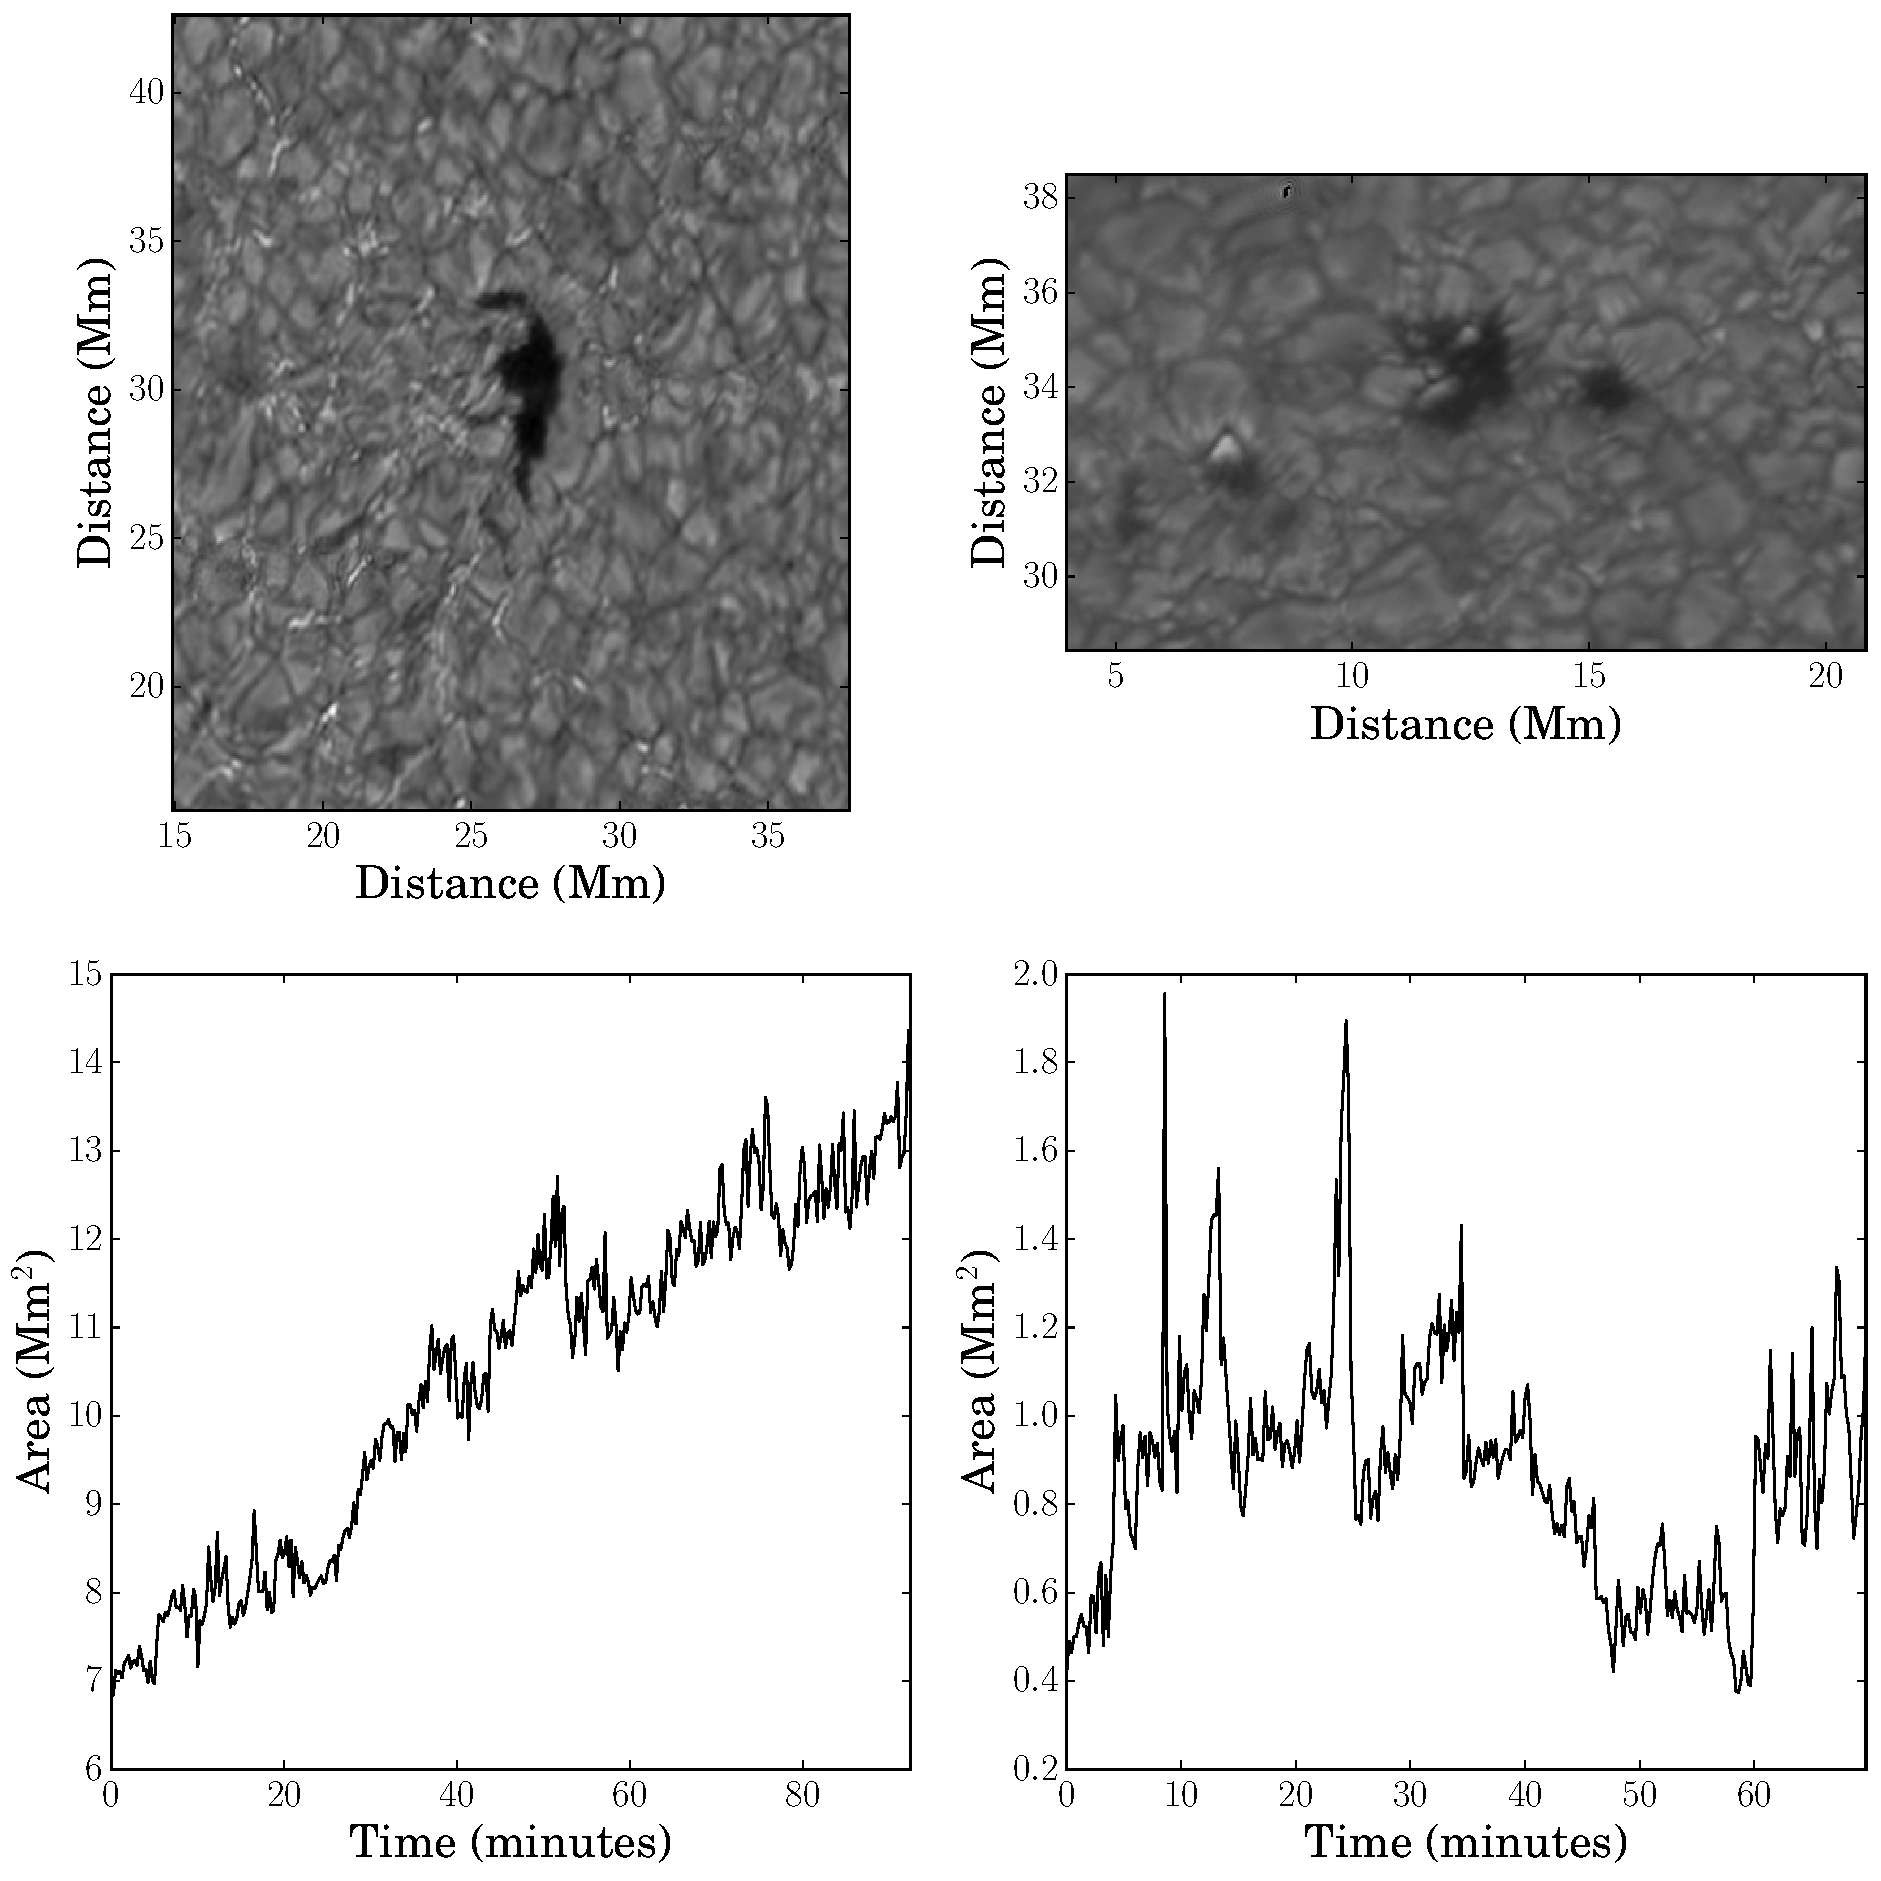
\includegraphics[width=\textwidth]{overview.pdf}
        \caption{
		         The left column displays the magnetic pore observed by the DOT while the right column is the magnetic pore observed by the DST/ROSA. 	
	        	 The magnetic pores at the start of the observation sequence (\textit{Upper panels}).
	             The original (trended) cross-sectional time series for each pore throughout the observation sequence. (\textit{Lower panels}).}
        \label{overview}
    \end{figure}
    
    Two high-resolution data sets are investigated within this article.
    The first data set was acquired using the Dutch Open Telescope (DOT) \citep{rutten}, located on La Palma in the Canary Islands. 
    The data were taken on $12$th August $2007$ with a G-band ($430.5$ nm) filter which samples the low photosphere and has a formation height of around $250$ km above the solar surface.
    The observation started at $08$:$12$ UTC and lasted for $92$ minutes with a cadence of $15$ seconds with a total field-of-view (FOV) of $60$ Mm by $40.75$ Mm.
    The DOT is able to achieve high spatial ($0.071''$ per pixel) resolution, due to the DOT reduction pipeline.
    It comes at a cost of temporal cadence which is decreased to $30$ seconds as data reduction uses speckle reconstruction \cite[]{1992A&A...261..321K}.
    Note, that the DOT does not have an adaptive optics system.
    
    The second data set was obtained on the $22$nd August $2008$ with the Rapid Oscillations in the Solar Atmosphere (ROSA) imaging system situated at the Dunn Solar Telescope (see \citealt{jess1} for details on experimental setup and data reduction techniques).
    Observation started at $15$:$24$ UTC, and data were taken using a $417$ nm bandpass filter with a width of $0.5$ nm.
    The $417$ nm spectral line corresponds to the blue continuum that samples the lower photosphere and the formation height of the filter wavelength corresponds to around $250$ km above the solar surface.
    It should be noted that this is an average formation height. 
    This is because the contributions to the line are from a wide range of heights and the lines also form at different heights depending on the plasma properties \citep{gband}.
    
    ROSA has the ability for high spatial ($0.069''$ per pixel) and temporal ($0.2$ s) resolutions.
    After processing through the ROSA pipeline the cadence was reduced to $12.8$ s to improve image quality via speckle reconstruction \citep{20764}.
    To ensure alignment between frames, the broadband time series was Fourier co-registered and de-stretched \citep{2007A&A...473..943J}.
    Count rates for intensity are normalised by the ROSA pipeline.
    
    The methodology of this analysis follows the method that was also applied by \citet{morton2011} and \cite{Dorotovic2014}.
    The area of the pore is determined by summing the pixels that have intensity values that are less than $3\sigma$ of the median background intensity, which is a large quiet-Sun region. 
    This method contours the pore area well, but not perfectly, as the intensity between the pore and the background granulation is not a hard boundary.
    The top row of Figure \ref{overview} shows the magnetic pores at the start of the observation sequence, by DOT and ROSA, respectively. 
    Furthermore, the output from the area analysis is shown in the bottom row for both magnetic pores.
    A strong linear trend can be observed for the DOT pore.
    The intensity time series was determined by the total intensity of all the pixels within the pore.
    To search for periodic phenomena in the time series, two data analysis methods were used: wavelets and EMD.
    The wavelet analysis employs an algorithm that is a modified version of the tool developed by \citet{torrence}.
    The standard Morlet wavelet, which is a plane sine wave with the amplitude modulated by a Gaussian function, was chosen due to its high resolution in the frequency domain.
    The EMD code employed here is the one used by \citet{terradas}.
    First, we de-trended each time series by linear regression followed by wavelet analysis to determine the periodicity of the oscillations as a function of time.
    Second, cross-wavelet is applied to calculate the phase difference between the area and intensity series as a function of time.
    Although it is possible to obtain a better visual picture of the phase relation between the two signals by using EMD, the results agreed with the cross-wavelet analysis when checked. 
    
\section{MHD wave theory}
\label{Wave}
    
    \subsection{The sausage mode}
    \label{Saus}
    
    We aim to identify MHD sausage modes, so, it is important to have a theoretical understanding of these modes.
    Assume that a magnetic pore is modelled adequately by a cylindrical waveguide with a straight background magnetic field, i.e., $\textbf{B}_0=B_0\hat{\textbf{z}}$.
    We	note that, for reasons of clarity, in the following discussion the theory does not take gravitational effects on wave propagation into account.
    However, the influence of gravity may be important for wave propagation in magnetic pores, especially at the photospheric level where the predicted scale height is comparable to the wavelengths of observed oscillations.
    Therefore we should be cautious with the interpretations.
    The velocity perturbation is denoted as $\textbf{v}_1= (v_r,v_{\theta},v_z)$.
    From the theory of ideal linear MHD waves in cylindrical waveguides, for the $m=0$ modes (here, $m$ is the azimuthal wavenumber) i.e., for axisymmetric perturbations, the equations determining $v_r$ and $v_z$ decouple from the governing equation of $v_{\theta}$.
    Hence, we will have magnetoacoustic modes described by $v_r$ and $v_z$ and the torsional Alfv\'en mode is described by $v_{\theta}$.
    We are interested in the slow magnetoacoustic mode in this paper, so we neglect the $v_{\theta}$ component.
    The	same applies to the component of the magnetic field in the $\theta$-direction. 
    The linear magnetoacoustic wave motion is then governed by the following ideal MHD equations,
    \begin{align}
        &&\rho_0 \frac{\partial v_r}{\partial t}=-\frac{\partial}{\partial r}
        \left(p_1+\frac{B_0b_z}{\mu_0}\right)+\frac{B_0}{\mu_0}\frac{\partial b_r}{\partial z},
        \label{eq:mom_r}\\
        &&\rho_0\frac{\partial v_z}{\partial t}=-\frac{\partial p_1}{\partial z},
        \label{eq:mom_z}\\
        &&\frac{\partial b_r}{\partial t}=B_0\frac{\partial v_r}{\partial z},
        \label{eq:mag_r}\\
        &&\frac{\partial b_z}{\partial t}=-B_0\frac{1}{r}\frac{\partial (rv_r)}{\partial r},
        \label{eq:mag_z}\\
        &&\frac{\partial p_1}{\partial t}=-\rho_0
        c_s^2\left(\frac{1}{r}\frac{\partial(rv_r)}{\partial r}+\frac{\partial v_z}{\partial z}\right),
        \label{eq:press1}\\
        &&\frac{\partial \rho_1}{\partial t}=-\rho_0\left(\frac{1}{r}\frac{\partial (rv_r)}{\partial r}+\frac{\partial v_z}{\partial z}\right).
        \label{eq:den}
    \end{align}
    Here, $p$ is the gas pressure, $\rho$ is the density and $\textbf{b} = (b_r,b_{\theta},b_z)$ is the perturbed magnetic field.
    We have assumed that the plasma motion is adiabatic.
    The subscripts $0$ and $1$ refer to unperturbed and perturbed states, respectively.
    
    Now, assume that the wave is harmonic and propagating and let $v_r=A(r)\cos(kz-\omega t)$.
    We then obtain the following equations for the perturbed variables,	
    \begin{align}
        &&\omega b_r=-B_0kv_r,\label{eq:n0}\\
        &&\rho_0\left(\frac{v_A^2k^2}{\omega}-\omega\right)A(r)\sin(kz-\omega t)=\frac{\partial}{\partial r}\left(p_1+\frac{B_0b_z}{\mu_0}\right)
        &&\label{eq:n1}\\
        &&\rho_0\frac{\partial v_z}{\partial t}=-\frac{\partial p_1}{\partial z},
        \label{eq:n2}\\
        && b_z=\frac{B_0}{\omega}\frac{1}{r}\frac{\partial (rA(r))}{\partial r}\sin(kz-\omega t),
        \label{eq:n3}\\
        &&\frac{\partial p_1}{\partial t}=c_s^2\frac{\partial\rho_1}{\partial t}=-\rho_0 c_s^2\left(\frac{1}{r}\frac{\partial(rv_r)}{\partial r}+\frac{\partial v_z}{\partial z}\right)
        \label{eq:n4}
    \end{align}
    Integrating Equation (\ref{eq:n4}) with respect to $t$ and using Equation (\ref{eq:n2}) (which is also integrated with respect to $t$) gives
    \begin{align}
        &&p_1=c_s^2\,\rho_1=-\frac{\omega\rho_0
            c_s^2}{(c_s^2k^2-\omega^2)}\frac{1}{r}\frac{\partial
            (rA(r))}{\partial r}\sin(kz-\omega t).
        \label{eq:n5}
    \end{align}
    The full derivation can be found in Appendix 1.
    Comparing Equation (\ref{eq:n3}) to Equation (\ref{eq:n5}), it can be noted that the magnetic field, $b_z$, and the pressure (density) are $180$ degrees out of phase.
    This depends on the sign of $c_s^2k^2-\omega^2$, which is assumed to be positive.
    Consideration of Equations \ref{eq:n1}, \ref{eq:n3} and \ref{eq:n5} leads to the conclusion that $v_r$ is $90\degree$ out of phase with $b_z$ and $-90\degree$ out of phase with $p_1$.
    
    The flux conservation equation for the perturbed variables gives the following relation,
    \begin{align}
        &&B_0S_1=-b_{1z}S_0,
        \label{eq:flux}
    \end{align}
    where $S$ refers to the cross-sectional area of the flux tube.
    We conclude that the perturbation of the area is out of phase with the perturbation of the  z-component of the magnetic field, hence, the area is in phase with the fluctuations of the thermodynamic quantities.
    Perhaps more importantly, we re-write Equation (\ref{eq:flux}) as
    \begin{align}
        &&\frac{S_1}{S_0}=-\frac{b_{1z}}{B_0}.
        \label{eq:mag_area}
    \end{align}
    Hence, if we are able to measure oscillations of a pore's area, we can calculate the percentage change in the magnetic field due to these oscillations (assuming conservation of flux in the pore).
    This was previously suggested by \cite{0004-637X-806-1-132}.
    Exploiting this relation will allow a comparison to be made between the observed changes in pore area and the magnetic oscillations found from Stokes profiles (e.g. \citealp{Balthasar2000}).
    Furthermore, as there are known difficulties with using the Stokes profiles, observing changes in pore area could provide a novel way of validating or refuting the observed magnetic oscillations derived from Stokes profiles.
    These simplified phase relations were confirmed in a more complicated case by e.g., \cite{Moreels2013} and \cite{Moreels2013b}, who also derived the phase relations for other linear MHD waves. 
    
    By measuring the change in pore area with time, we will also be able to estimate the amplitude of the radial velocity perturbation.
    The changes in area are related to changes in the radius of the flux tube by
    \begin{align}
        &&\frac{S_1}{S_0}=\frac{2r_1}{r_0},
        \label{eq:area_rad}
    \end{align}
    where $r_0$ and $r_1$ are the unperturbed radius and perturbation of the radius, respectively, assuming the flux tube has a cylindrical geometry.
    Once a periodic change in radius is identified, the radial velocity of the perturbation can then be calculated using the following relation
    \begin{align}
        &&v_r=\frac{\partial r}{\partial t}=\frac{2\pi r_1}{P}.
        \label{eq:rad_vel}
    \end{align}
  
  	Note the term ``sausage mode'' was introduced for waves in magnetic tubes with a circular cross-section.
  	The main property of these waves that distinguishes them from other wave modes is that they change the cross-sectional area.
  	The cross sectional areas of observed pores are typically non-circular.
  	However, it seems to be reasonable to use the term sausage mode for any wave mode that changes the cross-sectional area.
  	Several preceding papers have looked into non-circular, e.g., elliptic shapes, and found the effects to be marginal on the MHD waves within these tubes (see \citealt{2009A&A...494..295E} and \citealt{2011A&A...527A..53M}).
  	  
    \subsection{Period ratio of standing slow MHD wave}
    \label{stand}
    
    The period of a standing wave in a uniform and homogeneous flux tube is given by $P \approx 2L/nc_{ph}$, where $L$ is the tube length, $n$ is a integer determining the wave mode harmonics and $c_{ph}$ is the phase speed of the wave.
    This ratio is for ideal homogeneous tubes, however, this is not the case for the solar atmosphere from the photosphere to the transition region.
    \citet{luna-cardozo} modelled the effect of density stratification and expansion with the height of the flux tube on the ratio of the fundamental and first overtone periods for a vertical flux tube sandwiched between the photosphere and transition region.
    Their analysis studied the slow standing MHD sausage mode and assumed a thin flux tube with a small radial expansion with height. 
    They investigated two cases; case one is where the flux tube undergoes weak magnetic expansion with constant density, finding,  
    \begin{align}
        &&\frac{\omega_{2}}{\omega_{1}}= 2 - \frac{15}{2}\frac{\beta_{f}}{(6+5\beta_{f})\pi^{2}}(\Gamma-1),
        \label{mag_strat}
    \end{align}
    where $\omega_{i}$ is the period of specific harmonic or overtone (i.e., 1, 2), $\beta_{f}$ is the plasma-$\beta$ at the base of the flux tube and $\Gamma$ is the ratio of the radial size of the flux tube at the apex to the foot-point.
    Here, Equation (\ref{mag_strat}) is Equation (43) from \cite{luna-cardozo}.
    Case two is where the flux tube has density stratification but a constant vertical magnetic field, finding,
    \begin{align}
        &&\frac{\omega_{2}}{\omega_{1}}= \left[\frac{16\pi^{2} + \displaystyle\left(\ln\frac{1 - \sqrt{1 - \kappa_{1}}}{1 + \sqrt{1 - \kappa_{1}}}\right)^{2}}{4\pi^2 + \displaystyle\left(\ln\frac{1 - \sqrt{1 - \kappa_{1}}}{1 + \sqrt{1 - \kappa_{1}}}\right)^{2}} \right]^{1/2},
        \label{den_strat}
    \end{align} 
	where $\kappa_{1}$ is the square root of the ratio of the density at the top of the flux tube to the density at the footpoint ($\kappa_{1} = (\rho_{apex}/\rho_{footpoint})^{0.5}$).
    Here, Equation (\ref{den_strat}) is Equation (40) from \cite{luna-cardozo}.
    The upper end of the flux tube may well be the transition region while the footpoint is in the photosphere.
    It should be noted that the form of Equation (\ref{den_strat}) depends on the longitudinal density profile; a density profile where the tube speed increased linearly with height was used in this analysis.
 
    This may or may not model a realistic pore and given the uncertainty of the equilibrium quantities this must be kept in mind in order to avoid over-interpretation.
    Both Equations (\ref{mag_strat}) and (\ref{den_strat}) modelling the frequency ratio of standing oscillations indicate that the ratio of the first harmonic to the fundamental will always be less than two for flux tube expansion while the density stratification could increase this value.
    Furthermore, the thin flux tube approximation is used to derive these equations.
    Obviously, in a real flux tube, both the density and magnetic stratification would be present at the same time and would alter the ratio.
    This is not accounted for at the moment.
    Finally, Equations (\ref{mag_strat}) and (\ref{den_strat}) are independent of height, which may limit the results, as it has been suggested that the height to the transition region varies \citep{tian2009solar}.	
    
\section{Results and discussion}
\label{res}

    \begin{sidewaysfigure}
        \centering
        \begin{subfigure}[b]{0.45\textwidth}
            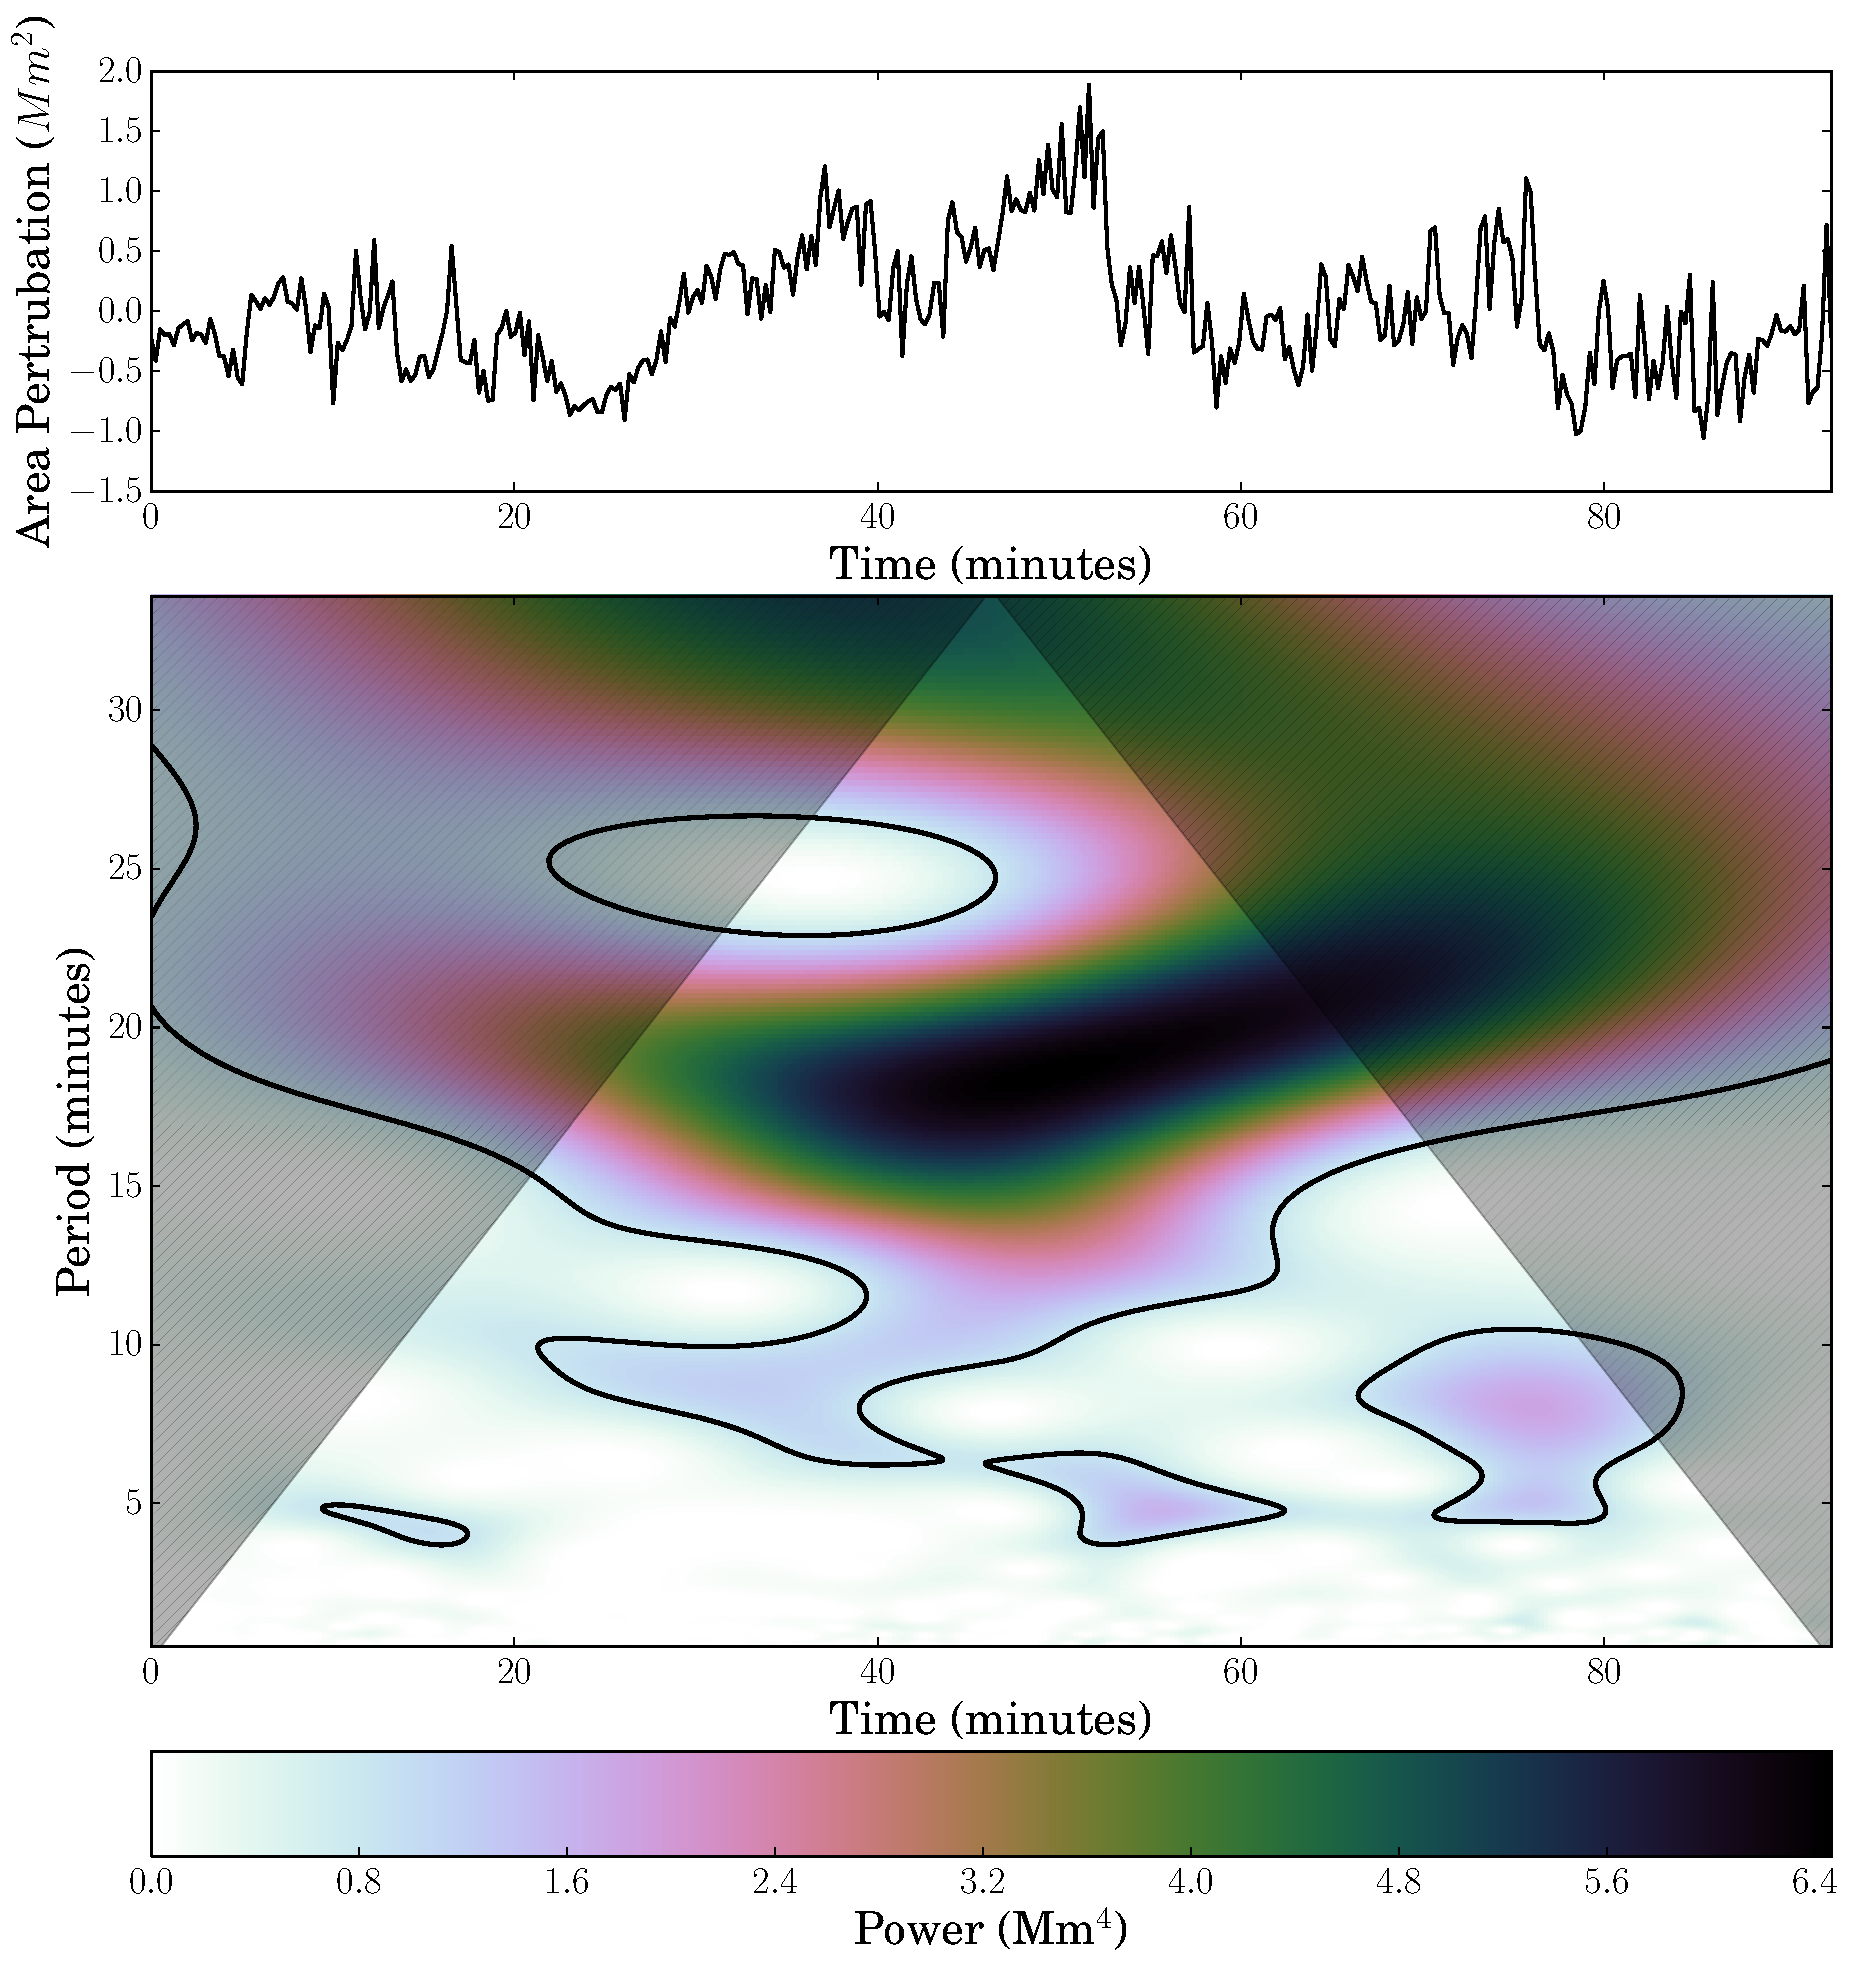
\includegraphics[width=\textwidth]{dot_area.pdf}
        \end{subfigure}
        \begin{subfigure}[b]{0.45\textwidth}
            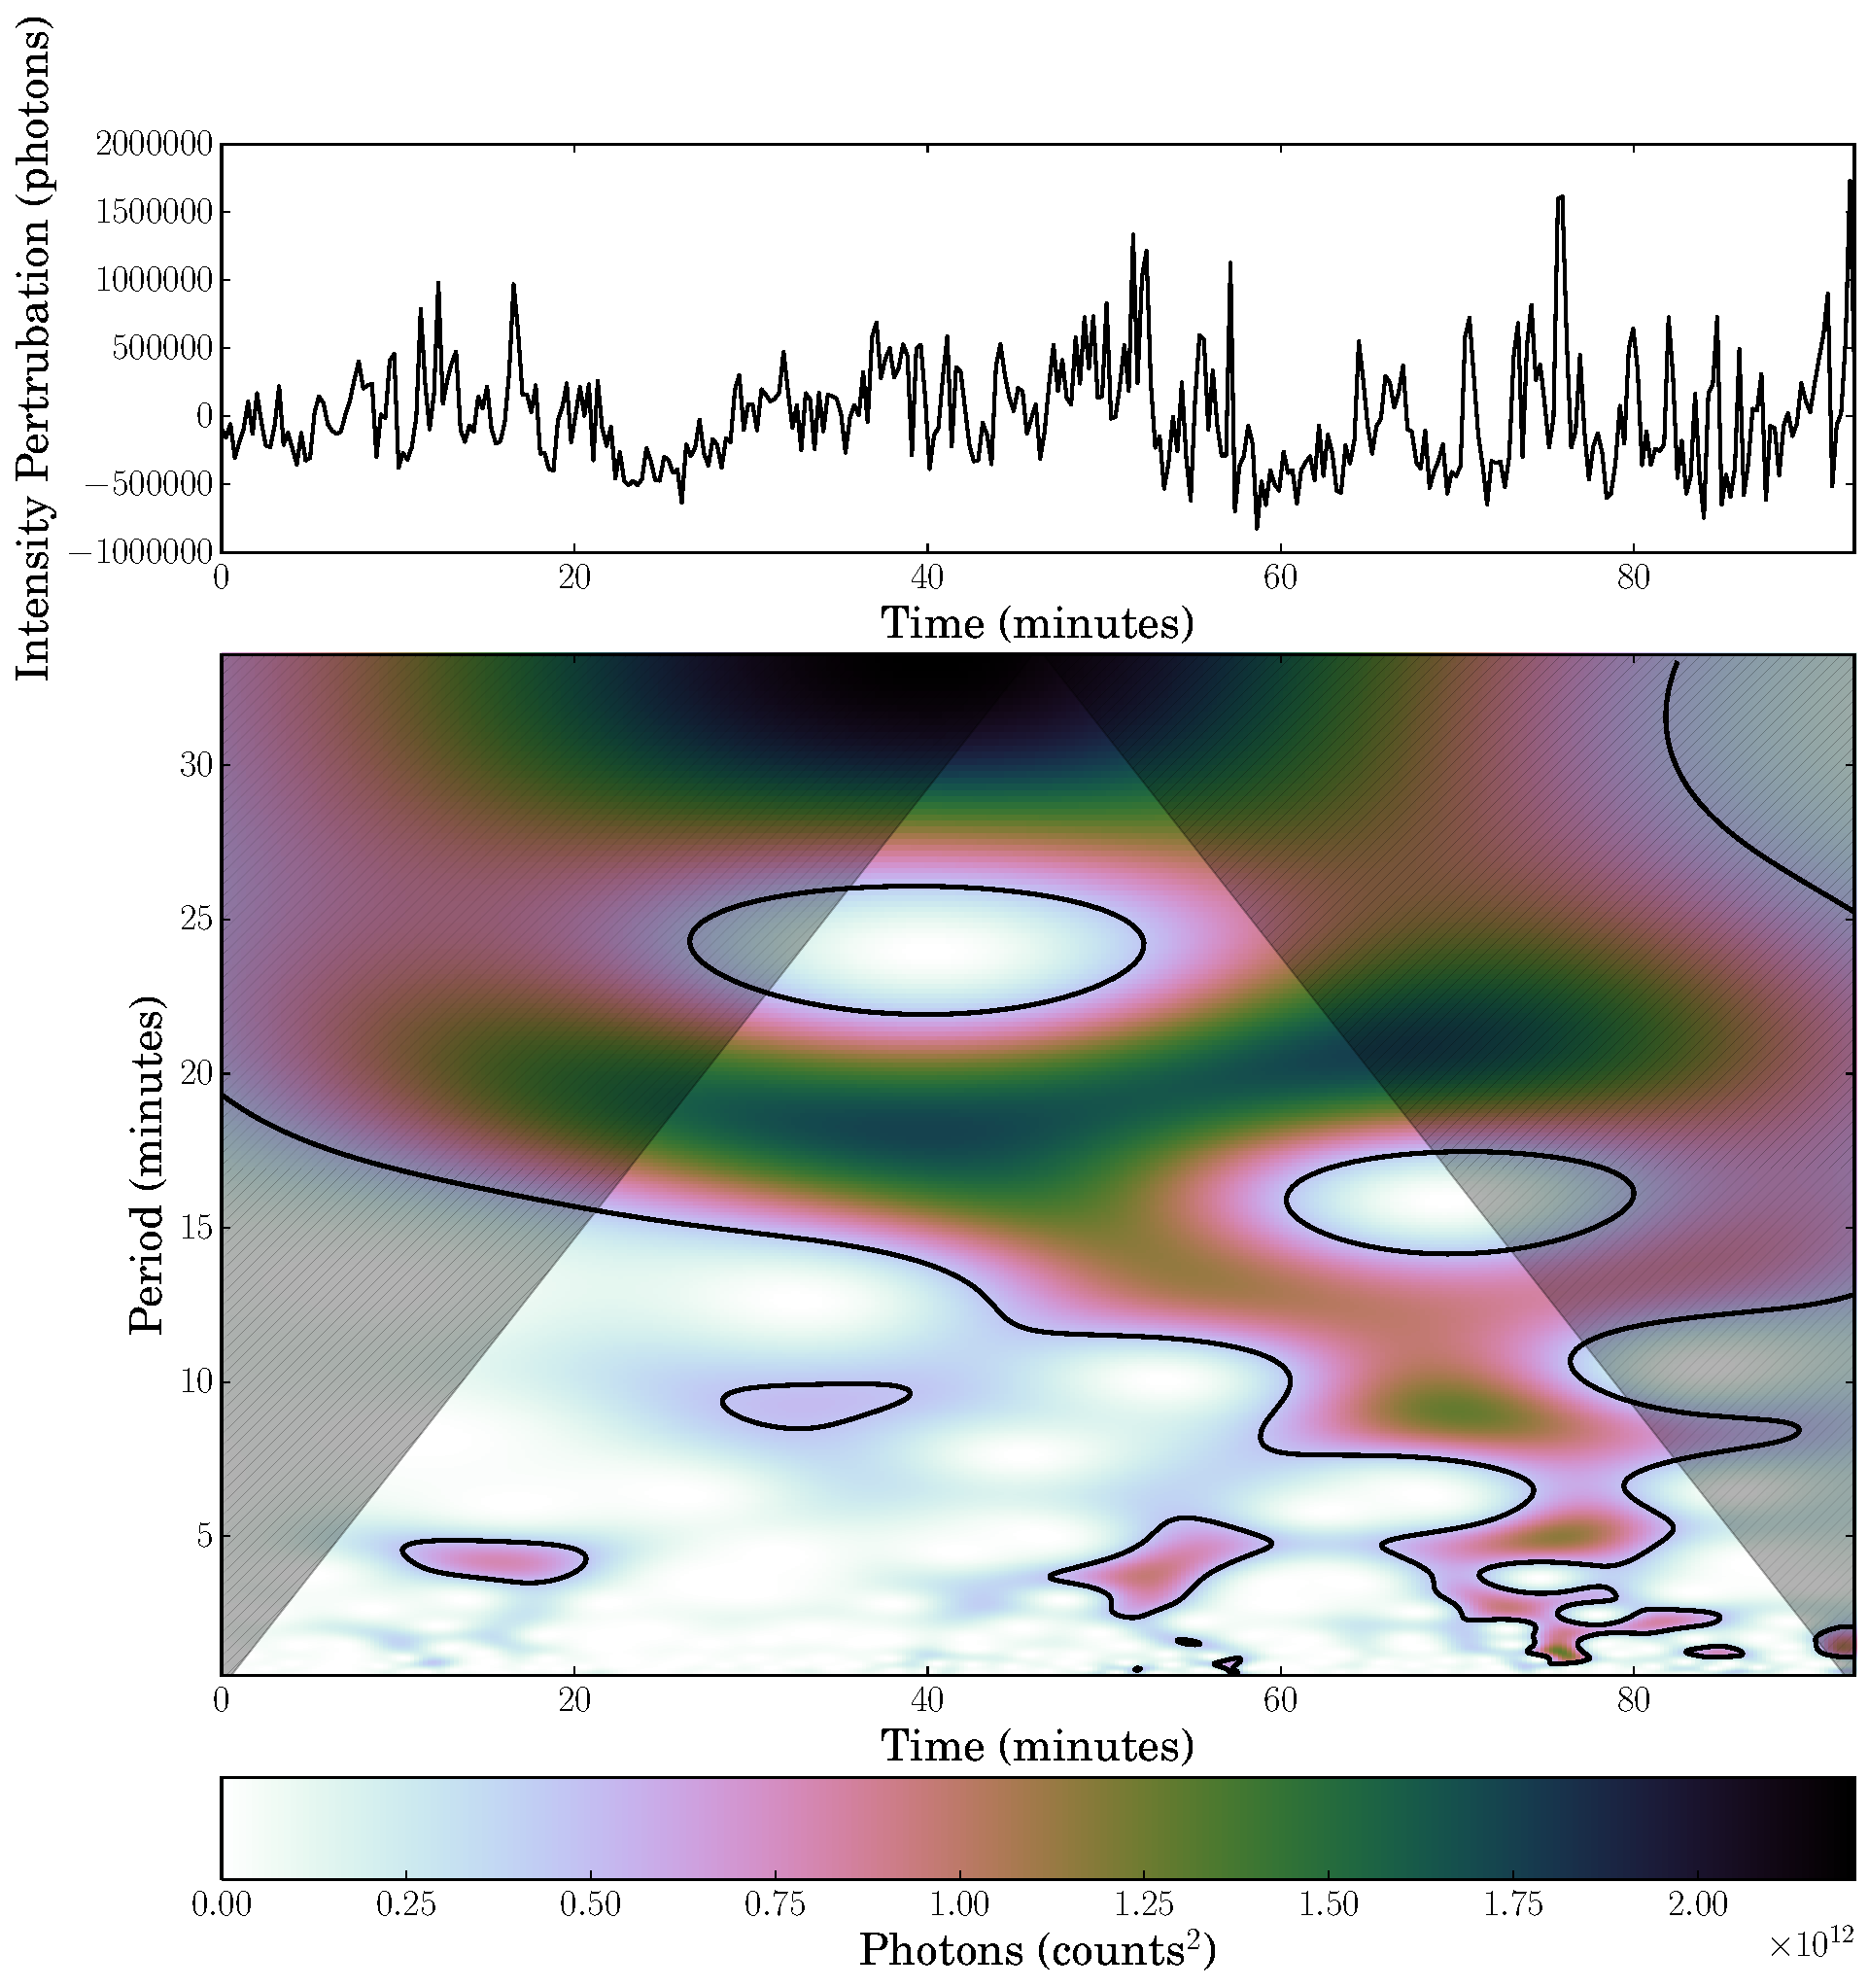
\includegraphics[width=\textwidth]{dot_inten.pdf}
        \end{subfigure}
        \caption{Evolution of the area of the pore observed with DOT (\textit{Upper panels}).
            The corresponding wavelet power spectrum for a white noise background.
            The cone of influence is marked as the shaded region and the contour lines show the 95\% confidence level (\textit{Lower panels}).}
        \label{DOT_wls}
    \end{sidewaysfigure}
    
    \begin{sidewaysfigure}
        \centering
        \begin{subfigure}[b]{0.45\textwidth}
            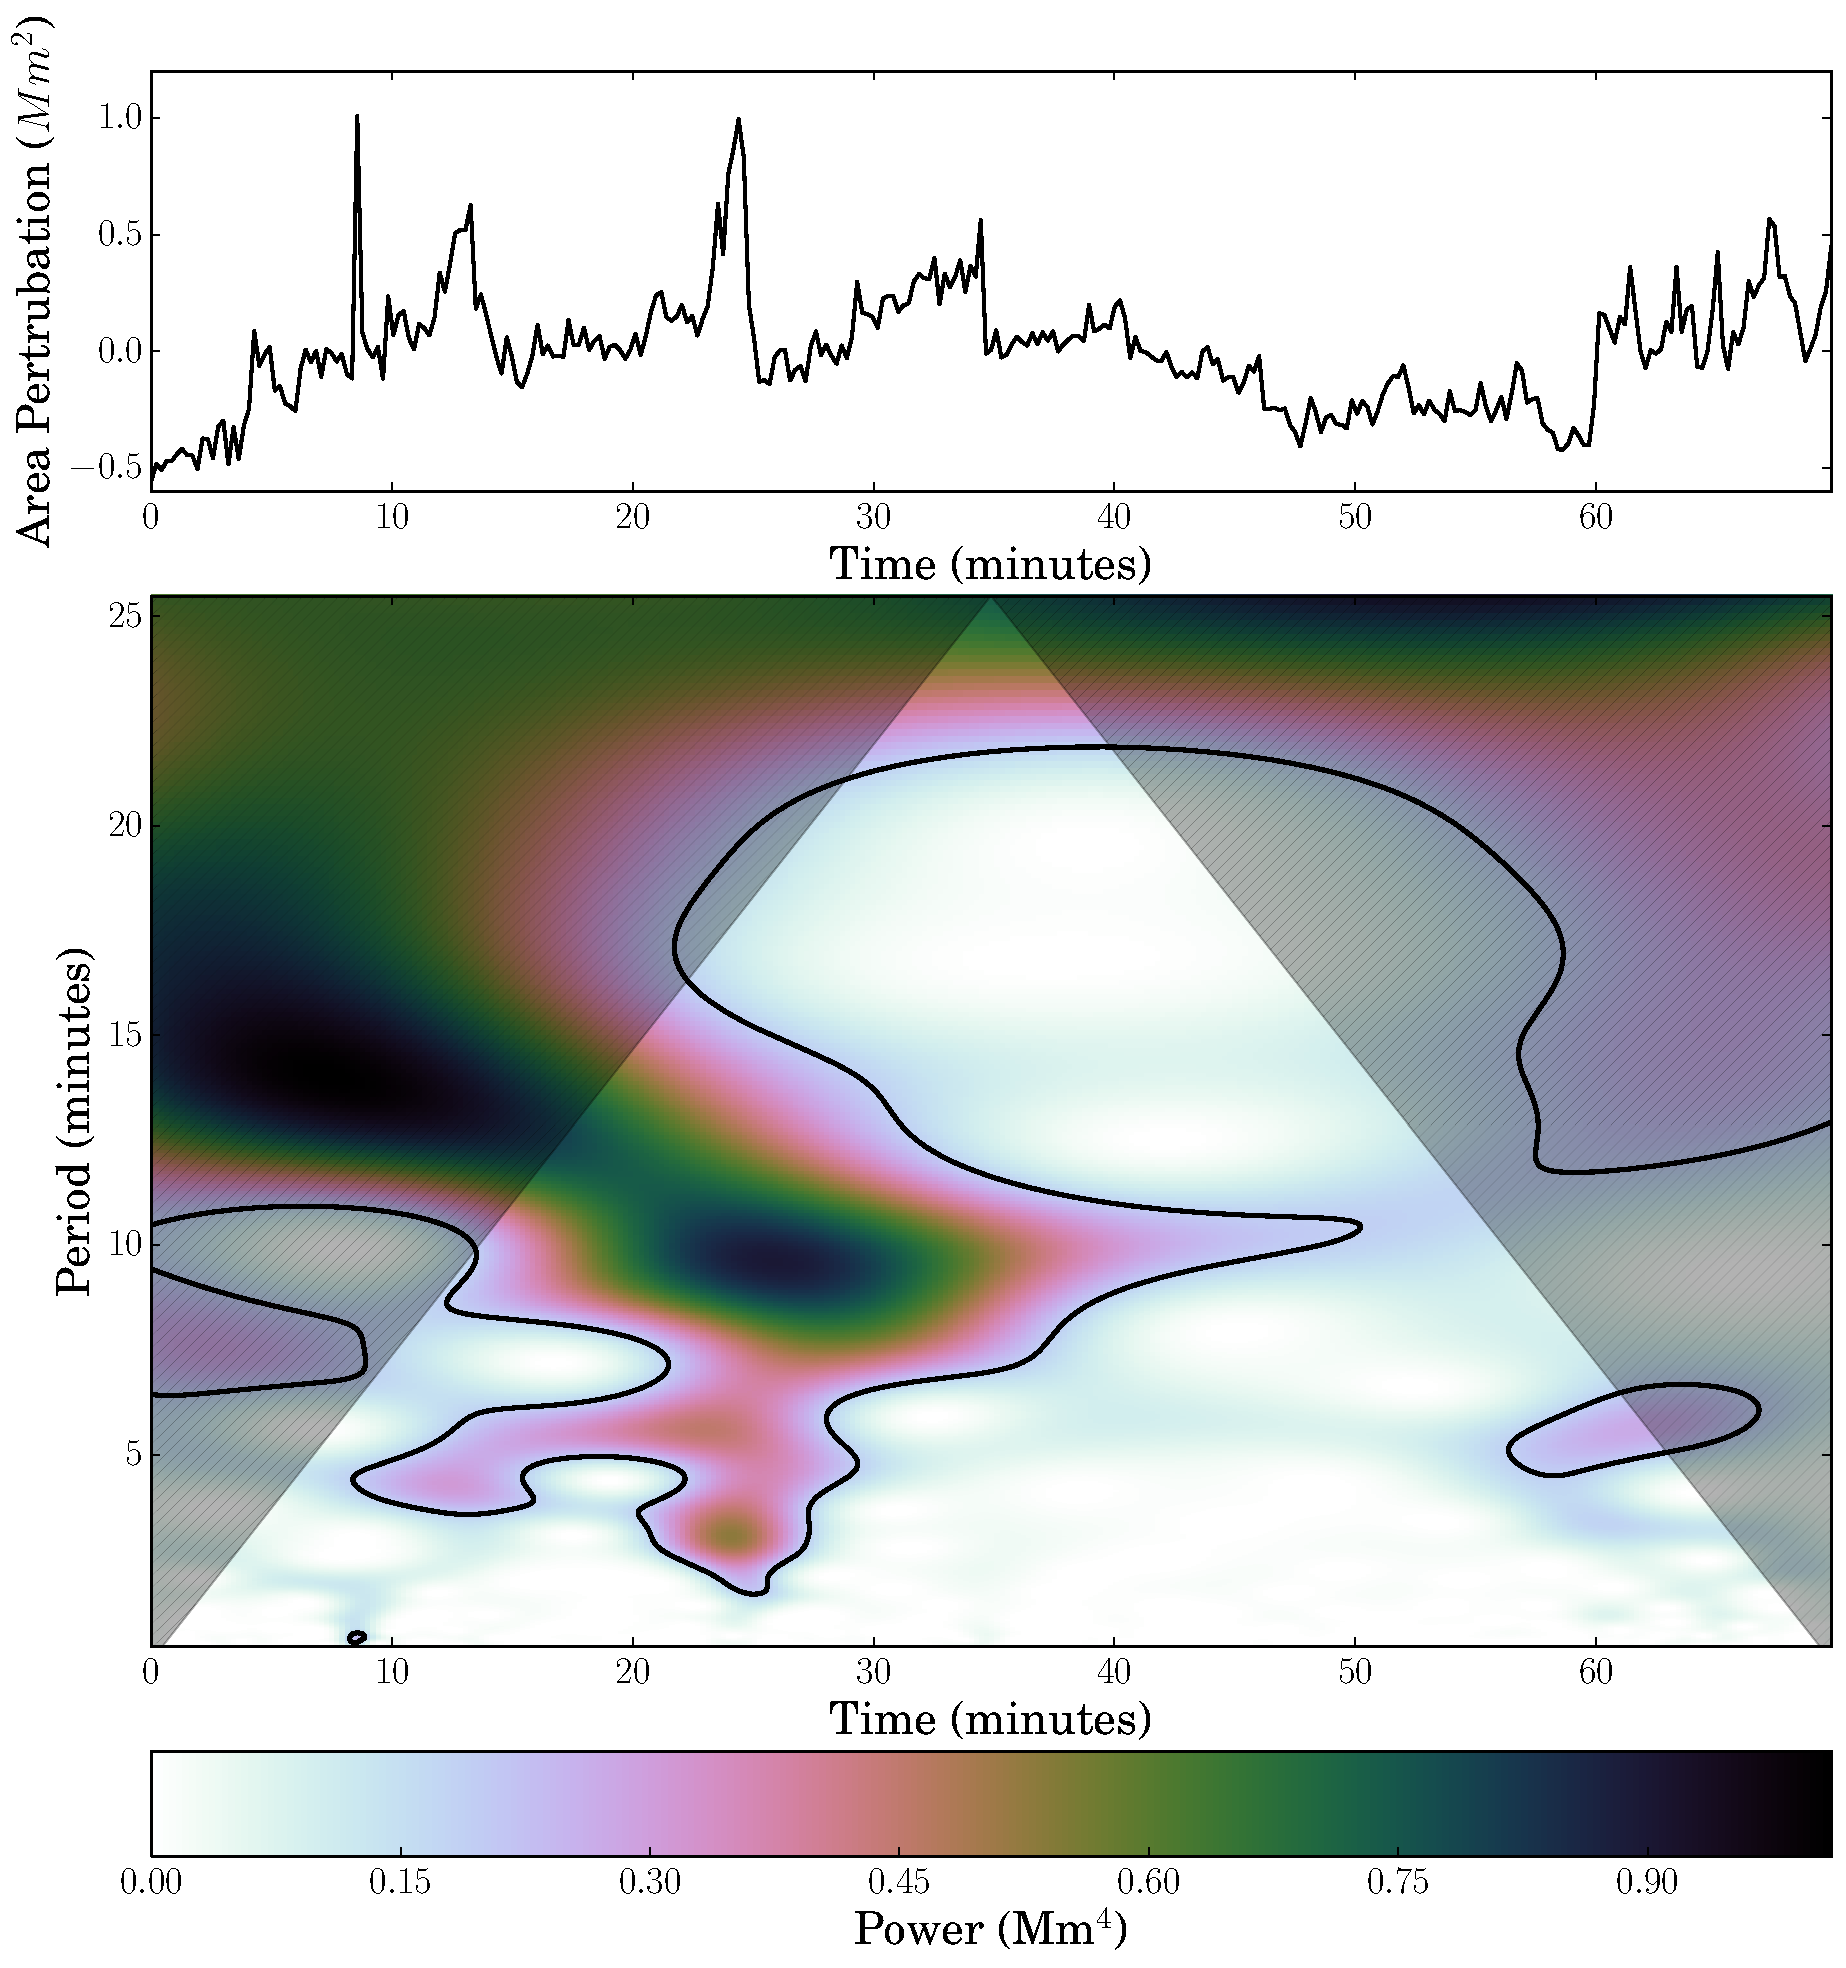
\includegraphics[width=\textwidth]{rosa_area.pdf}
        \end{subfigure}
        \begin{subfigure}[b]{0.45\textwidth}
            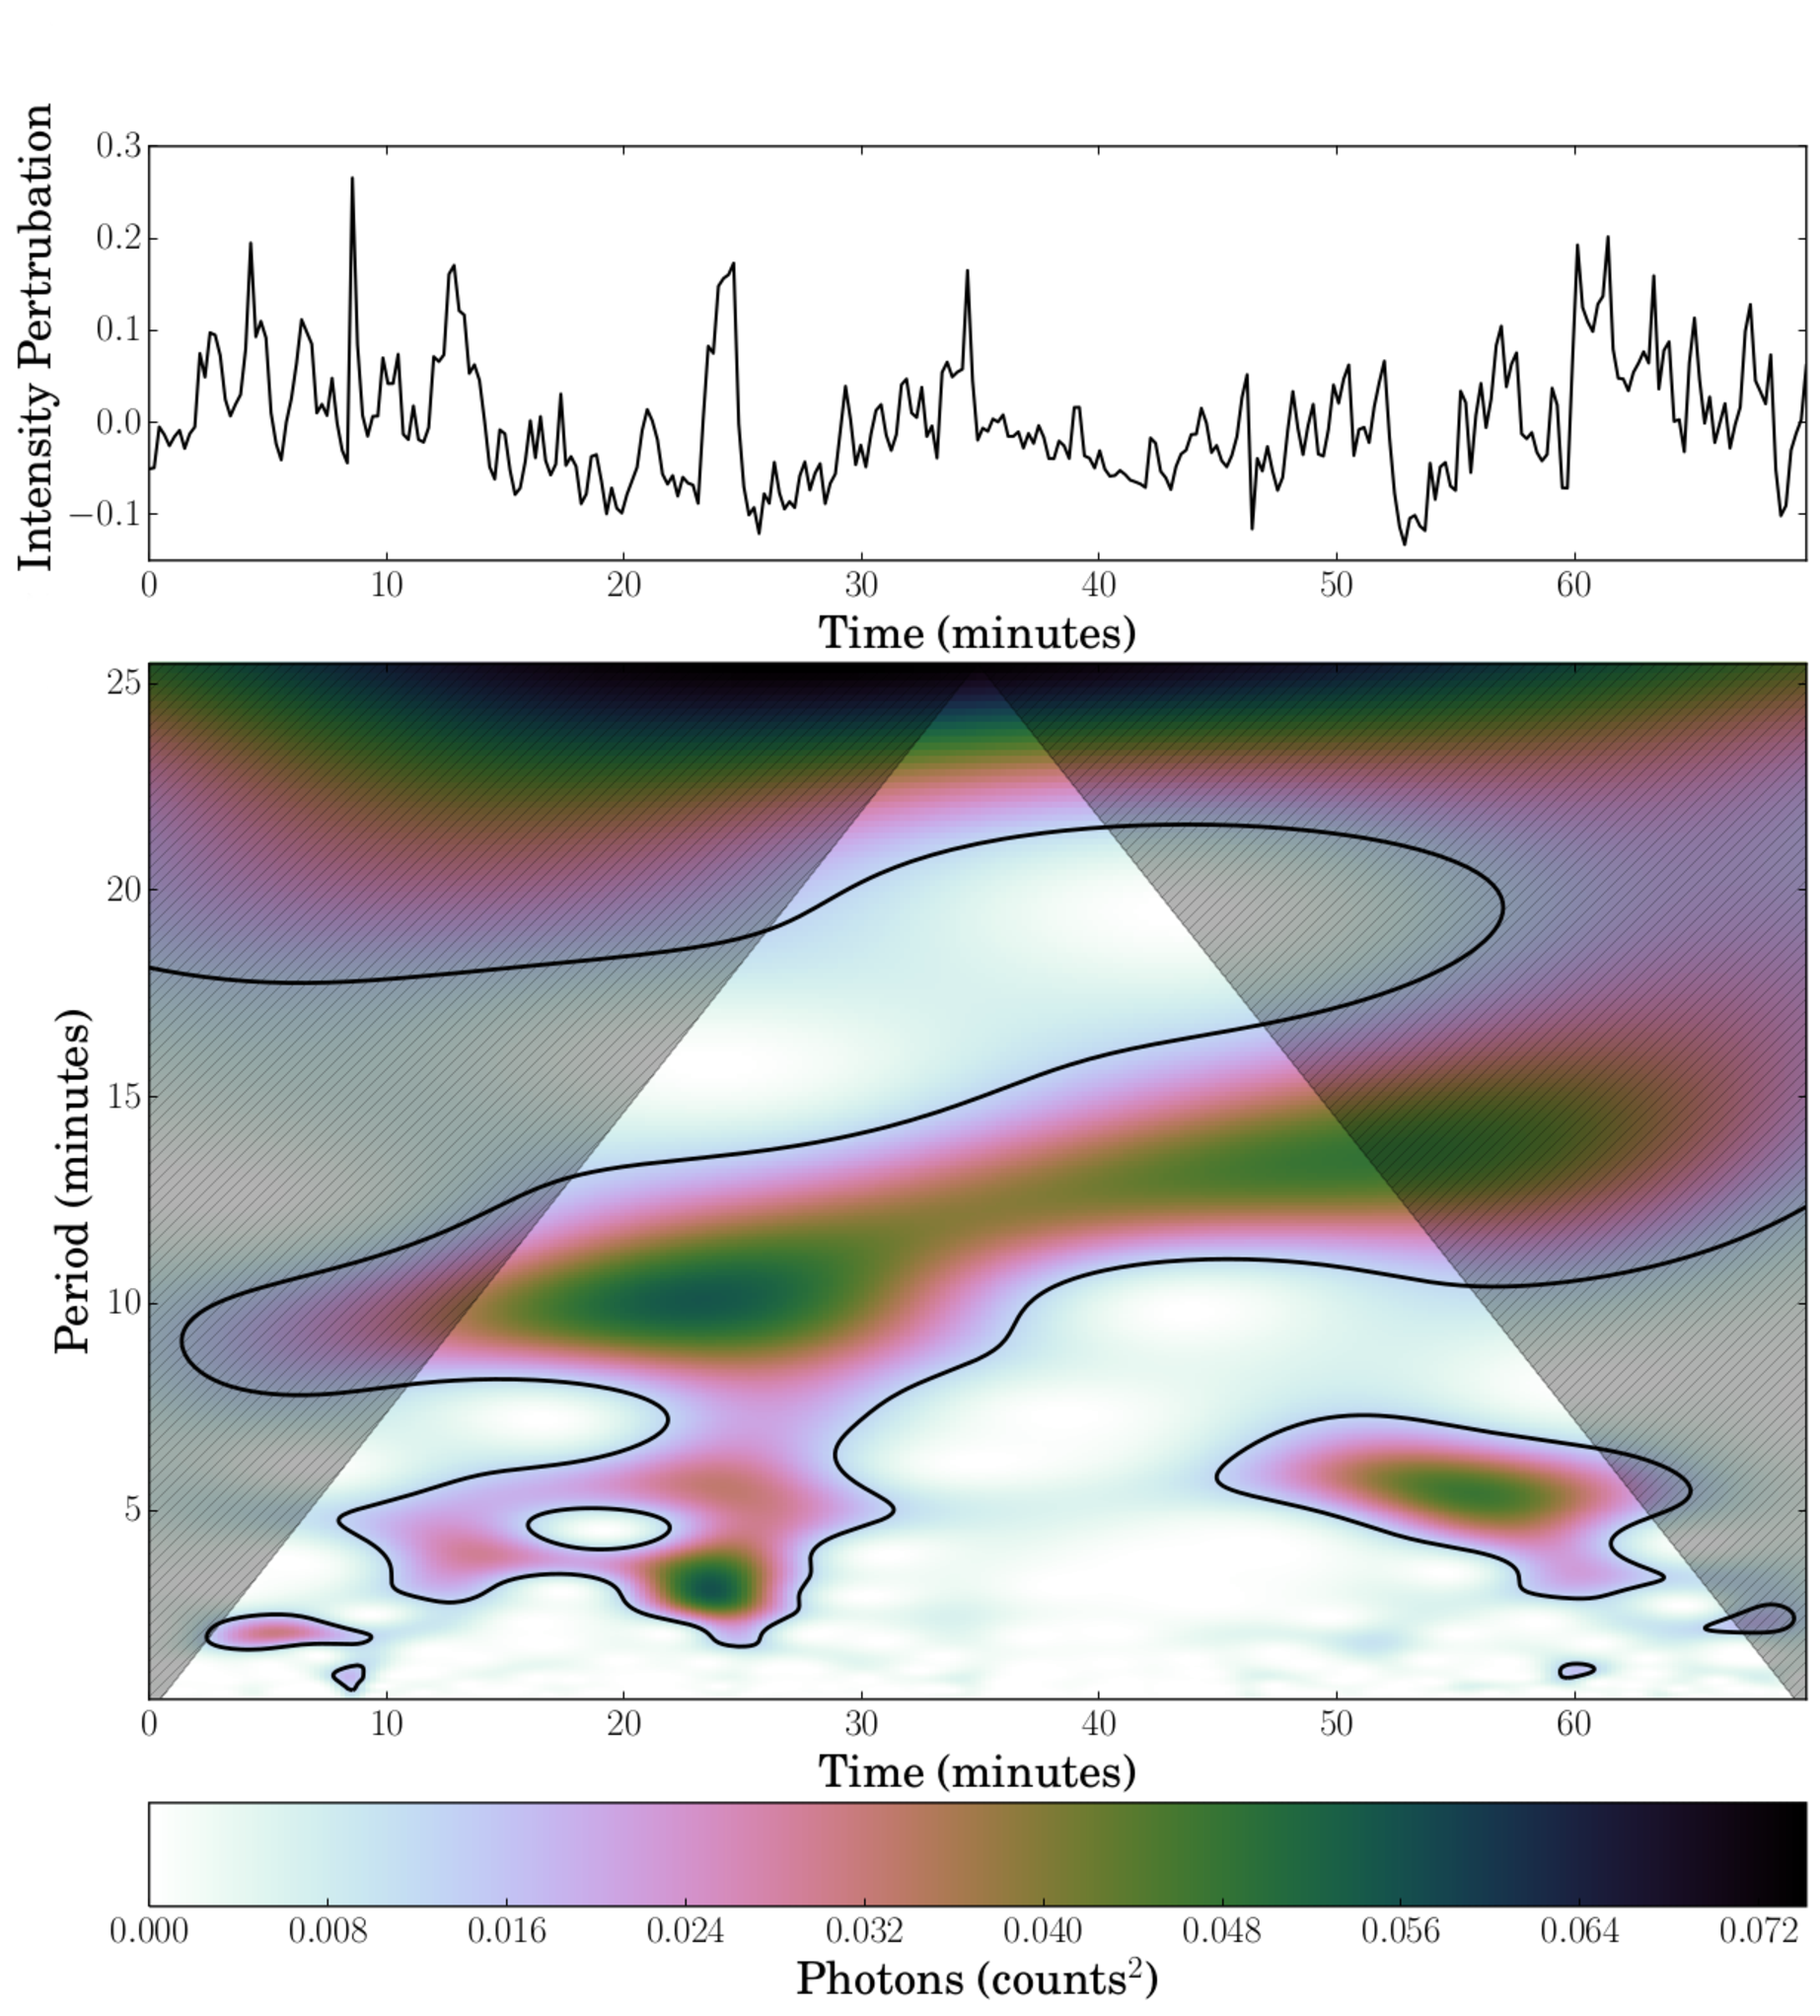
\includegraphics[width=\textwidth]{rosa_inten.pdf}
        \end{subfigure}
        \caption{Same as Figure \ref{DOT_wls} but for the pore observed with ROSA. Note that the intensity counts are normalised by the ROSA reduction pipeline \citep{jess1}.}
        \label{ROSA_wls}
    \end{sidewaysfigure}
    
    Figures \ref{DOT_wls} and \ref{ROSA_wls} show the results of a wavelet analysis of the area and intensity time series for the DOT and DST telescopes, respectively.
    The original signal is displayed above the wavelet power spectrum and the shaded region marks the cone of influence (COI), where edge effects of the finite length of the data affect the wavelet transform results.
    The contours show the confidence level of 95\%. 
    
    \subsection{DOT pore}
    
    There are four distinct periods found in the area time series of the pore; 4.7, 8.5, 20 and 32.6 minutes.
    The last period is outside the COI due to the duration of the time series, so it has been disregarded.
    It should be noted that periods of 8, 14 and 35 minutes have been observed in sunspots by \citet{kobanov}.
    This is important because magnetic pores and sunspots share a number of common features.
    The intensity wavelet shows 4 periods of oscillations; 4.7, 8.6, 19.7, and 35 minutes.
    These periods are similar, if not the same as the period of the area oscillations, which enables a direct comparison of the two quantities. 
    There is significant power that is co-temporal, which can be observed in both the intensity and area wavelets.
    
    Using cross-wavelet in conjunction with the EMD allows the verification of the phase difference between the area and intensity signals for each period. 
    These methods show that the phase difference is very close to 0\degree, i.e., the oscillations are in phase meaning that they are slow sausage MHD waves.	
    Furthermore, the percentage change in intensity is also of the same order as reported in \citet{Balthasar2000} and \citet{PMHDW}.
    This suggests that, we are most likely observing the same oscillatory phenomena as these authors.
    
    We also have to be certain that any change in area we observe is due to the magnetoacoustic wave rather than a change in the optical depth of the plasma.
    \citet{PMHDW} provide an insight into the expected differences between the phase of magnetic field and intensity oscillations due to waves or the opacity effect.
    They demonstrate that the magnetic field (pore area) should be in phase (out of phase) with the intensity if the oscillations are due to changes in optical depth.
    We note that this is the same relationship expected for the fast magnetoacoustic sausage mode.
    Hence, the identification of the fast magnetoacoustic mode in pores may prove difficult with only limited data sets.
    
    The application of Equations (\ref{eq:area_rad}) and (\ref{eq:rad_vel}) require information about the amplitude of the area perturbation.
    This can be achieved using either an FFT power spectrum or the IMF's amplitude from the EMD analysis.
    Here, we use EMD for the amplitudes (which are time-average values) and they are $3.87\mathrm{x}10^5$ km$^2$, $3.61\mathrm{x}10^5$ km$^2$ and $5.90\mathrm{x}10^5$ km$^2$ for the oscillations with periods of 4.7, 8.5 and 20 minutes, respectively.
    It was not possible to find the amplitude of the largest period, as it did not appear in the EMD output.
    The values of the area perturbation translate, using Equation (\ref{eq:area_rad}), to 37, 34, and 56 km, respectively, for the amplitude of the radial perturbation.
    Note that the increase in radius is about $100$ km, meaning that the perturbation is only of the order of 1 pixel (at the DOT's resolution).
    
    Using the values above allows us to calculate the radial velocity perturbation for each period, by means of Equation (\ref{eq:rad_vel}).
    For the periods of 4.7, 8.5, and 20 minutes, we determine the radial velocity perturbation as 0.82, 0.42, and 0.29 km s$^{-1}$, respectively.
    The obtained radial speeds are very sub-sonic, as the sound speed is $\approx$ 10 km s$^{-1}$ in the photosphere.
    They are, however, of order of observed horizontal flows around pores.
    
    Furthermore, it is also possible to estimate the percentage change in the magnetic field that is expected from the identified linear slow MHD sausage modes.
    The percentage change in pore area, hence magnetic field, is found to be $$\frac{A_1}{A_0} = \frac{b_1}{B_0} \rightarrow 4-7\%.$$
   	For another magnetic pore, the percentage change was found to be similar at 6\% \citep{0004-637X-806-1-132}.
    Let us now assume that the equilibrium magnetic field strength of the pore takes typical values of 1000-2000 G.
    Then, the amplitude of the magnetic field oscillations should be 40-140 G.
    The lower end of this estimated range of percentage change in the magnetic field agrees well with percentage changes in the magnetic field obtained using Stokes profiles by, for example, \citet{Balthasar2000} and \citet{PMHDW}.
    However, the upper end of the range, i.e. $\sim 140$ G, appears twice as large as any of the previously reported periodic variations in the magnetic field. 
    This apparent difference could be due to the spatial resolution of the magnetograms averaging out the magnetic field fluctuations.
    A summary of our findings can be found in Table \ref{tab:ampl}.
    
    \begin{sidewaystable}
        \centering
        \begin{tabular}{cccc|cccc}
            DOT & $r_{1}$ & $v_{r_1}$ & $\frac{b_{z1}}{B_{0}}$ & ROSA & $r_{1}$ & $v_{r_1}$ & $\frac{b_{z_1}}{B_{0}}$ \\ \hline \hline
            \begin{tabular}[c]{@{}l@{}}Period 1\\ 4.7 mins\end{tabular} & 37 km & 0.82 km s$^{-1}$ & 4.34\% & \begin{tabular}[c]{@{}l@{}}Period 1\\ 2-3 mins\end{tabular} & 69.1 km & 3.03 km s$^{-1}$ & 26.3\% \\
            \begin{tabular}[c]{@{}l@{}}Period 2\\ 8.4 mins\end{tabular} & 34 km & 0.42 km s$^{-1}$ & 4.04\% & \begin{tabular}[c]{@{}l@{}}Period 2\\ 5.5 mins\end{tabular} & 74.2 km & 1.41 km s$^{-1}$ & 28.2\% \\
            \begin{tabular}[c]{@{}l@{}}Period 3\\ 19.7 mins\end{tabular} & 56 km & 0.29 km s$^{-1}$ & 6.60\% & \begin{tabular}[c]{@{}l@{}}Period 3\\ 10 mins\end{tabular} & 117 km & 1.23 km s$^{-1}$ & 44.5\% \\
        \end{tabular}
        \caption{
	        	 The properties of each observed period for the DOT and ROSA data respectively.
                 $r_{1}$ is the radial perturbation, $v_{r1}$ is the velocity perturbation and $\frac{b_{z1}}{B_{0}}$ is the magnetic field perturbation.
                 These quantities are determined by using Equations \ref{eq:area_rad} and \ref{eq:rad_vel}
                 }
        \label{tab:ampl}         
      \begin{tabular}{cccc|cccc}
            	DOT & $\lambda_z$ & $k_z$ & $k_{z}a$ & ROSA & $\lambda_z$ & $k_z$ & $k_{z}a$ \\ \hline \hline
            	\begin{tabular}[c]{@{}l@{}}Period 1\\ 4.7 mins\end{tabular} & 1269 km & 4.95 $\mathrm{x}10^{-6}$ m$^{-1}$ & 8 & \begin{tabular}[c]{@{}l@{}}Period 1\\ 2-3 mins\end{tabular} & 540-810 km & 7.76-12 $\mathrm{x}10^{-6}$ m$^{-1}$ & 4-6\\
            	\begin{tabular}[c]{@{}l@{}}Period 2\\ 8.4 mins\end{tabular} & 2268 km & 2.77 $\mathrm{x}10^{-6}$ m$^{-1}$ & 5 & \begin{tabular}[c]{@{}l@{}}Period 2\\ 5.5 mins\end{tabular} & 1485 km & 4.2 $\mathrm{x}10^{-6}$ m$^{-1}$  & 2\\
            	\begin{tabular}[c]{@{}l@{}}Period 3\\ 19.7 mins\end{tabular} & 5319 km & 1.18 $\mathrm{x}10^{-6}$ m$^{-1}$ & 2 & \begin{tabular}[c]{@{}l@{}}Period 3\\ 10 mins\end{tabular} & 2700 km & 2.33 $\mathrm{x}10^{-6}$ m$^{-1}$ & 1 \\
         \end{tabular}    
         \caption{
		          The wavelength (wavenumber) for each observed period for the DOT and ROSA data respectively.
               	  Here, $k=2\pi/\lambda$ and $\lambda=v/f$, where $k$ is the wavenumber, $\lambda$ is the wavelength, $v$ is the velocity and $f$ is the frequency.
               	  }
      	\label{tab:wavelength}      	  
    \end{sidewaystable}
    
    Now we estimate the wavelength (wavenumber) for each mode.
    An important fact needs to be remembered, i.e., the velocity perturbation determined is radial, not vertical.
   	Furthermore, since the waveguide is strongly stratified, we define the wavelength as the distance between the first two nodes, which is the half wavelength of the wave.	
    However, in this regime, the vertical phase speed of the slow sausage MHD wave is the tube speed, which is $c_T\approx4.5$ km s$^{-1}$ using typical values for the photospheric plasma \citep{WPMC,evans}.
    For the periods of $4.7$, $8.5$ and $20$ minutes we obtain estimates of the wavelength (wavenumber) as $1269$ km ($4.95\mathrm{x}10^{-6}$ m$^{-1}$), $2268$ km ($2.77\mathrm{x}10^{-6}$ m$^{-1}$) and $5319$ km ($1.18\mathrm{x}10^{-6}$ m$^{-1}$), respectively.
    Note that these wavelengths are larger than the scale height in the photosphere ($\approx 160$ km)  or the lower chromosphere.
    For the observed pore, it had an average radius, $a=1.5$ Mm, where $ka= 8, 5, 2$.
    See Table \ref{tab:wavelength} for a summary.
   
    \subsection{ROSA pore}
    
    There are four distinct periods found in the area time series of the pore observed by ROSA; 2-3, $5.5$, $10$ and $27$ minutes.
    All of these reported periods are at least at the $95\%$ confidence level (or over).
    A few words about two of the periods have to be mentioned.
    First, the power of the $2$-$3$ minute period is spread broadly, and, as such it is hard to differentiate the exact period.
    Secondly, the $10$-minute period slowly migrates to $13.5$ minutes as the time series comes to its end.
    The intensity wavelet shows four periods of oscillations; 2-3, 5.5, 10, and 27 minutes.
    For the pore observed by DOT, the oscillations found in the area and intensity data share similar periods.
    Also, there is another period that is below the $95\%$ confidence level for white noise at 1-2 minutes at the start of the time series.
    This is a similar behaviour as found for the DOT pore.
    
    We found that the phase difference between the area and intensity periods is 0\degree.
    This means, as before, that these oscillations are in phase and are interpreted as signatures of slow sausage MHD waves.
    While we have chosen not to discuss the out of phase behaviour, there are small regions of 45$\degree$ phase difference that have been previously reported \citep{Dorotovic2014}.
    This needs to be investigated in the future, as the authors are unaware of which MHD mode would cause this behaviour, however, it has been suggested that is due to noise within the data set \citep{2015A&A...579A..73M}.
    As for the DOT pore, the same properties can be obtained for each period observed as within the ROSA pore, which are summarized in Table \ref{tab:ampl} and \ref{tab:wavelength}.
    
	The amplitudes for the area oscillations are $2.29\mathrm{x}10^5$ km$^2$, $2.45\mathrm{x}10^5$ km$^2$, and $3.87\mathrm{x}10^5$ km$^2$ for periods of 2-3, 5.5, and 10 minutes, respectively.
	The $13.5$-minute period is found by the EMD process as well, and has an amplitude that is the same as that of the $10$-minute period. 
	Again, it was not possible to find the amplitude of the largest period.
	These then, lead to the radial perturbation amplitude of 69.1, 74.2, and 117 km and a radial velocity perturbation as 3.03, 1.41, and 1.23 km s$^{-1}$, respectively.
	The increase in radius is around $100$ km meaning that the perturbation is only of the order of 2 pixels (at ROSA's resolution).
	This means that for each part of the structure, its radius increases by 2 pixels.
	Once again, the radial velocity perturbations are found to be sub-sonic.
	
    The percentage change in the pore's area, and thus the magnetic field, is given by $$\frac{A_1}{A_0} = \frac{b_1}{B_0} \rightarrow 25 - 45\%.$$
    From the above relations we conclude that the size of the magnetic field oscillation is in the region of $200$-$400$ G.
    This is a substantial increase when compared to the measurements of the pore detected by DOT, as the amplitudes for these oscillations are of the same order but the cross-sectional area of the pore is an order of magnitude smaller.
    This suggests that the oscillation strength might be independent of the scale of the structure \citep{Dorotovic2014}. 
    
    Once again, we determine the wavelength (wavenumber) for each period, using the tube speed as defined in the previous section.
    For the periods of $2-3$, $5.5$, and $10$ minutes we obtain estimates of the wavelength (wavenumber) as $540$-$810$ km ($7.76\mathrm{x}10^{-6}$ m$^{-1}$), 1485 km ($3.58\mathrm{x}10^{-6}$ m$^{-1}$), and 2.2 Mm ($2.85\mathrm{x}10^{-6}$ m$^{-1}$), respectively.
    For the observed pore radius, $a=0.5$ Mm, we obtain values of $ka = 2, 1.8, 1.5,$ and $1.5$.
    
    \subsection{Standing oscillations}
    
    \begin{table*}
        \centering
        \begin{tabular}{cc|cc}
            DOT Period (Mins) & Ratio ($P_{1}/P_{i}$) & ROSA Period (Mins) & Ratio ($P_{1}/P_{i}$)\\ \hline \hline
            \begin{tabular}[c]{@{}l@{}}\end{tabular} 8.5 mins & - & \begin{tabular}[c]{@{}l@{}}\end{tabular} 10 mins & - \\
            \begin{tabular}[c]{@{}l@{}}\end{tabular} 4.7 mins & 1.81 & \begin{tabular}[c]{@{}l@{}}\end{tabular} 5.5 mins & 1.81 \\
            \begin{tabular}[c]{@{}l@{}}\end{tabular}  & & \begin{tabular}[c]{@{}l@{}}\end{tabular} 2-3 mins & 3.3-5 \\
        \end{tabular}
        \caption{
            The periods of oscillations as well as the harmonic ratios for the DOT and ROSA magnetic pore respectively.
            The periods listed here exist at 95\% confidence level and are within the COI.
            Periods greater than $10$ minutes have been neglected.}
        \label{harm_table}
    \end{table*}
    
    \begin{figure}
        \centering
        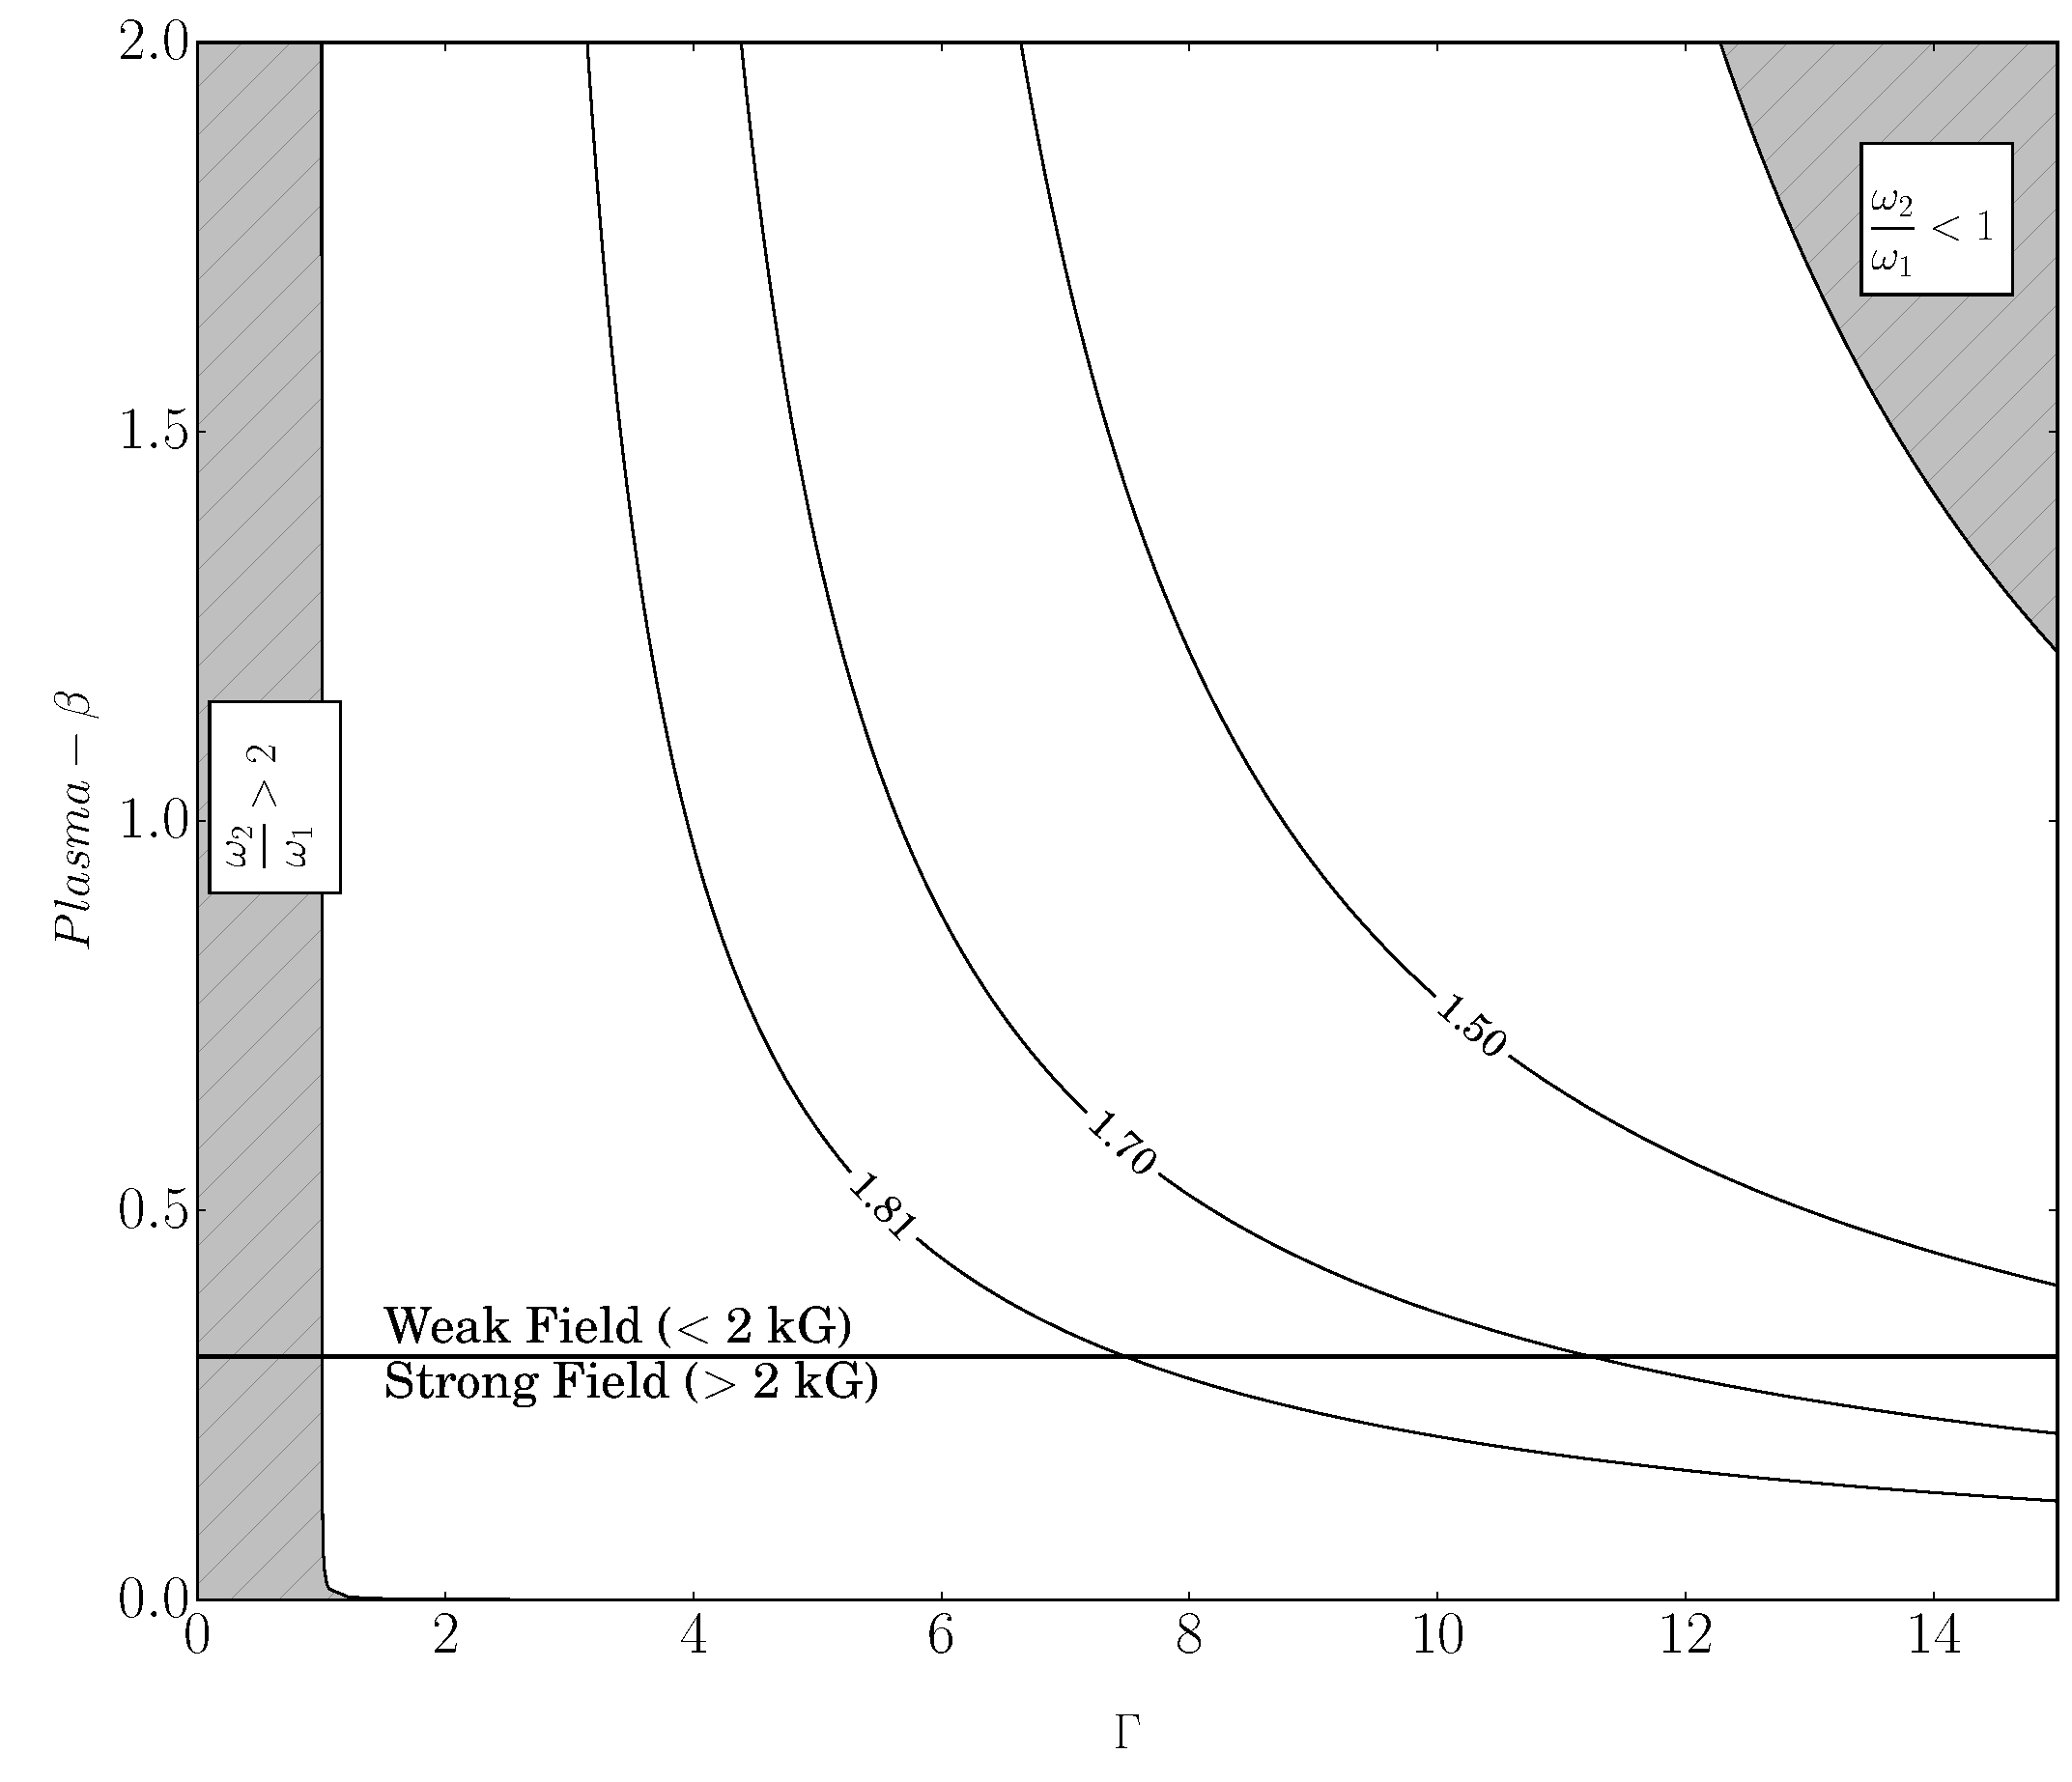
\includegraphics[width=\textwidth]{harmonics.pdf}
        \caption{The range of solutions for Equation (\ref{mag_strat}).
            The threaded areas are where the period ratios are either less than one or greater than two.
            The horizontal line divides the image into a weak ($<2$ kG) and strong ($>2$ kG) field regions for the plasma-$\beta$.
            The blue contour lines indicate observed period ratios for this paper and the values within \cite{Dorotovic2014}.}
        \label{fig:harm}
    \end{figure}		
    
    With the important understanding that the observed waves are trapped, there is a possibility of them being standing waves.
    Assuming that the pore can be modelled as a straight homogeneous magnetic flux tube that does not expand with height, the sharp gradients (often modelled as discontinuities) of the temperature/density at the photosphere and at the transition region form a resonant cavity that can support standing waves \citep[see][]{fleck,malins}.  
    
    Calculating the harmonic periods ($P \approx 2L/nc_{ph}$, where $L$ is the distance between the boundaries ($2$ Mm), $n$ is the harmonic number), a fast MHD oscillation ($c_{p}\approx12$ kms$^{-1}$) would have a fundamental period $\sim$333 s, while the period of a slow MHD wave ($c_{p}\approx5.7$ kms$^{-1}$) would be $\sim$700 s.
   	Other slow MHD sausage waves have been observed with phase speeds similar to this \citep{2015A&A...579A..73M}.
    The interpretation of the observed waves is that they are slow MHD sausage waves, which, in the ideal homogeneous case, is the most similar to the observed results; however, it is still different by two minutes.
    Therefore, the basic assumption of an ideal homogeneous flux tube (constant $L$, constant $c_{ph}$ etc.) is inadequate for explaining the results presented in this chapter.
    
    There are several further considerations that need to be taken into account.
    From observations, many magnetic structures are not cylindrical or symmetrical and are often irregular in shape.
    Furthermore, large-scale magnetic structures have been thought to be made up of either a tight collection of small-scale flux tubes or one large monolithic structure \citep[][and the references within]{priest1984solar}.
    Also, these magnetic structures extend from the photosphere to the transition region which means that the plasma-$\beta$ will vary by an order of $2$ magnitude, which will change the dynamics of the MHD waves considerably.
    We have also ignored the effect of gravity (i.e., density stratification \citealt{2006A&A...458..975D,2011ApJ...743..164A}), as well as the equally important fact that flux tubes expand with height, i.e., magnetic stratification, which alters the ratio of the periods, i.e, $P_{1}/P_{2}\neq2$ \citep{luna-cardozo}. 
    All of these effects will further affect the wave dynamics inside flux tubes.
    
	Here, we will ignore periods greater than $10$ minutes; as shown above in the ideal homogeneous case, the largest period possible is $11.6$ minutes for MHD waves (with the above assumptions).
	Here, we will consider two effects: the effect of density stratification and magnetic expansion with height in the radial direction.
	For the first case; Equation (\ref{den_strat}) is calculated with typical density values from the VAL-III C model \citep{1981ApJS...45..635V} at the apex (transition region) and footpoint (photosphere) of the flux tube.
	The VAL-III C model is an estimation of a quiet-Sun region and the interior density ratio between the photosphere and the transition region of a flux tube need not necessarily differ greatly from that of the exterior atmosphere (see Figures 3 and 1 of \citealp{GFME13a} and \citealp{GFE14}, respectively). 
	The resulting value for the period ratio in this instance is 1.44 (density values are $2.727\mathrm{x}10^{-7}$ and $2.122\mathrm{x}10^{-13}$ g cm$^{-3}$ for the footpoint and apex, respectively).
	Using the model given by \citet{Maltby1986}, which models a sunspot umbra, this period ratio is 1.38 (density values are 1.364$\mathrm{x}10^{-6}$ and 9.224$\mathrm{x}10^{-14}$ g cm$^{-3}$ for the footpoint and apex respectively).
	This does not correspond well to the results in this paper, but only for one previously reported result; a highly dynamical non-radially uniform sunspot \citep{Dorotovic2014}.
	The ratio is substantially smaller than what is detected here, which means the first harmonic should be at $\approx 5.9$ minutes.
	This model does not seem to be applicable to the observational results presented here. 
	The reason for this, the authors believe, is due to the effect of finite radius.
	The dispersion relation for slow MHD waves in a finite radial flux tube, shows that the dispersion related to the finite tube radius increases the wave frequency.
	The shorter the wavelength, the stronger the dispersion effect is.
	Hence, the relative increase of the first overtone frequency due to the effect of finite radius is larger than that of the fundamental harmonic.
	This modifies the period of the first harmonic to be higher, which shifts the period ratio to be larger than values that are obtained theoretically in the thin tube approximation.
    
    Figure \ref{fig:harm} details the various solutions (\textit{i.e.,} period ratio) for Equation (\ref{mag_strat}) over a large range of plasma-$\beta$ and expansion ratio ($\Gamma$).
    It is difficult to estimate how much a flux tube expands with height, therefore, we explore the parameter space widely, taking $\Gamma$ of 0-15.
    The values for the plasma-$\beta$ are divided into strong ($\geq2$ kG) and weak ($\leq2$ kG) field regions, as the magnetic field of flux tubes hypothesised, and will vary from $0.5$ kG to $4$ kG.
    The magnetic pores were observed before the launch of NASA's Solar Dynamics Observatory (SDO),
    so the best magnetic data comes from the Michelson Doppler Imager (MDI) instrument on board SOHO.
    As such, the magnetic field of these pores is hard to know precisely due to their small scale and MDI's large pixel size.
    However, ground-based observations of similar sized pores reveal magnetic fields ranging from $1$ kG to $2.5$ kG.
    The blue contour lines show the parameter space that matches the period ratios reported in this article and the ones in \citet{Dorotovic2014}.
    For example, if the plasma-$\beta$ is around 1, the expansion factors for the three period ratios reported here are around $4$, $6$, and $9$.
    If we have plasma-$\beta$ $\ll 1$, the expansion ratio starts to increase rapidly. 
    
    Once again, this effect can be dominant when the flux tube expands too much, however, it is unlikely that a flux tube would expand by such a large amount.
    \citet{1982GApFD21237B}, for example, suggest that when the internal gas pressure exceeds the external gas pressure, the flux tube becomes unstable and this occurs when the flux tube expands greatly with height.
    
    For the cases presented in this paper, the flux tube has to expand four to six times to have a period ratio that is observed.
    In a number of numerical simulations that model these types of flux tubes, the magnetic field expands approximately 4-10 times, which happens to be not too dissimilar to our findings \citep[see also][]{khomenko,fedun2,fedun1}.
    It should be noted that these estimates for expansion are for flux tubes with magnetic fields that have a field strength less than $2$ kG. 
    
    Unfortunately, as of yet, little is known about the source of the oscillations analysed in this paper.
    One possible origin of MHD sausage waves is suggested by e.g. \citet{khomenko} and \citet{fedun2}, where magnetoacoustic wave propagation in small-scale flux tubes was modelled using non-linear MHD simulations.
    One of the results of their simulations is that 5-minute vertical drivers can generate a mixture of slow and fast sausage modes in localised magnetic flux tubes that propagate upward.
    Furthermore, \citet{fedun1} model the effect of photospheric vortex motion on a thin flux tube, finding that vertex motions can excite dominantly slow sausage modes.
    However, these simulations need to be developed further before we may comfortably link them to our assertions.

	Another potential source is from mode conversion that will occur at the lower region of the photosphere within sunspots and magnetic pores.
	For example, \cite{0004-637X-746-1-68}, modelled a background sunspot-like atmosphere, and solving the non-linear ideal MHD equations for this system, found that the fast MHD wave will turn into a slow MHD sausage wave at the Alfv\'en-acoustic equipartition level (which is where the sound speed is equal the Alfv\'en speed) and the reverse is also true.
	The fast MHD wave to Alfv\'en conversion occurs higher up, where there is a steep Alfv\'en speed gradient, as the fast MHD wave will reflect from this boundary.
	Below this level, the MHD waves are fast and above this level, slow MHD waves can be supported.
	This level occurs at approximately 200 km in their model.
	The observations used within this paper are thought to form at a height around 250 km.
	Furthermore, sunspot umbras are depressed in height and it would likely be the same for magnetic pores.
	These facts can offer an insight into the formation height of G-band since we believe that we are observing a primary slow acoustic mode modified by the magnetic field i.e., the slow MHD sausage wave.
	    
    A word of caution: the absence of line-of-sight (LOS) Doppler data, it is difficult to know whether the oscillations reported are standing or propagating.
    The data available for magnetic pores does not cover higher levels of the solar atmosphere such as the chromosphere or the transition region.
    The data presented here only represents a slice of the flux tube near the photosphere.
    Future work is needed to acquire simultaneous observations of magnetic pores in several wavelengths in order to sample the solar atmosphere at different heights.
    Detailed spectral images would allow other LOS quantities such as Doppler velocity and magnetic field to be measured.
    This way, the oscillations could be determined confidently either as standing or propagating due to their different phase relations. 
    
    \section{Conclusions}
    \label{conc}
    
    The use of high-resolution data with short cadence, coupled with two methods of data analysis (wavelets and EMD), has allowed the observation of small-scale wave phenomena in magnetic waveguides situated on the solar surface.
    By studying the area and intensity perturbations of magnetic pores, it enables the investigation of the phase relations between these two quantities with the use of wavelets and EMD.
    The in phase ($0^\circ$ phase difference) behaviour reveals that the oscillations observed are indicative of slow sausage MHD waves. 
    Furthermore, with the amplitude of oscillations measured, several properties could be estimated; such as the amplitude of the magnetic field perturbation and the radial speed of the perturbation.
    The scale of the magnetic field perturbations that are caused by slow MHD waves is of the order $10$\% and has radial speeds that are sub-sonic when compared to the sound speed at the photosphere.  
    With the MHD mode of these waves identified, the obtained vertical wavelength indicates that the flux tubes would have a strong reflection at the transition region boundary, further indicating a chromospheric resonator. 
    Finally, the investigation of the period ratio of the oscillations suggests that the fundamental and first harmonic has been observed within these flux tubes.
    The period ratio observed, coupled with magneto-seismology, enabled an expansion factor to be calculated that was in very good agreement with values found in numerical models used for MHD wave simulations.
\graphicspath{{Chapter5/Figs/}}

\chapter[Upwardly Propagating Waves]{The detection of upwardly propagating waves in a magnetic pore\footnote{This chapter is based on \bibentry{freij2014}. Reproduced with permission from AAS}}
\label{chapter5}
	
   \vspace*{\fill}\par
   \pagebreak

\section{Introduction}

	How energy is transported from the lower solar atmosphere into the corona is an important question that has yet to be fully answered despite decades of research\citep{erdelyi2004heating,erdelyi2007heating,Taroyan2009}.
	The complex interactions between strong magnetic fields and powerful flows, the latter created by the interplay of gravity, convection and magnetic forces, leads to a number of dynamic phenomena throughout the atmosphere, such as magneto-hydrodynamic (MHD) waves \citep{WPMC}, which are theorised to supply energy into the corona.
	Strong inhomogeneities and steep gradients of key atmospheric properties (such as temperature and density) can lead to strong reflection of wave energy in the upper chromosphere.
	It has proved difficult to both observe \citep{Aschwanden2006,Marsh2006,Jess2009,Taroyan2009,McIntosh2011,Parnell2012,Morton2012,Wedemeyer2012,Mathioudakis2013} and simulate \citep{steiner1998,hasan2005,peter2006,erdelyi2007,ErdeyiFedun2010,Vigeesh2012} the propagation of energy from the lower atmosphere into the corona \citep{Vecchio2007,DePontieu2007,Zaqarashvili2009,DePontieu2011,mcintosh2012,Rutten2012}.

	The most basic model of MHD theory suggests that three distinct types of waves should manifest in the solar atmosphere; namely slow and fast magneto-acoustic and the widely sought-after Alfv\'en wave \citep{Banerjee2007,Jess2009,Suzuki2011,McLaughlin2011,McIntosh2011,Mathioudakis2013}.
	High spatial and temporal resolution observations carried out using modern ground- and space-based instrumentation have revealed a plethora of energetic, incompressible \citep{1999ApJ520880A,DePontieu2007,Jess2009}, compressible \citep{Morton2012}, and significantly more complicated \citep{DePontieu2011,Wedemeyer2012}, oscillations and flows.
	What has yet to be observed is the direct propagation of energy from the lower regions of the solar atmosphere into the corona raising the question as to whether any of these wave processes are actually heating the outer solar atmosphere.
    Here, we contribute to addressing this question.

	Running penumbral waves (RPWs) were originally thought to be evidence of horizontal wave propagation \citep{Zirin1972,Giovanelli1972,Bloomfiel2008} which traced the topology of the local magnetic field \citep{Zhugzhda1973,Nye1974} around large sunspots.
	Due to this assertion, RPWs have been largely ignored with regards to any potential injection of energy into the corona.
	More recently, it has been suggested that these events are, in fact, upwardly propagating waves (UPWs, \citealt{OASO,Bloomfiel2008,Jess2013}), which could facilitate the propagation of non-thermal energy into the corona.
	Here, we present the first observations of UPWs situated around a pore and demonstrate that these waves can indeed penetrate from the lower solar atmosphere into the corona, potentially making them an excellent candidate for plasma heating within solar Active Regions (ARs).

	Discussed here is the propagation of UPWs through the plasma surrounding a large pore structure.
	By conducting a multi-wavelength, multi-instrument analysis, we are able to trace upward propagating wave-fronts from the chromosphere into the transition region (TR) and corona, estimating key properties such as apparent horizontal and vertical velocities, and non-thermal energy supply.
	The chapter is organised as follows: Section \ref{sect1} details the collection and reduction of the data presented; Section \ref{sect2} describes the analysis of the data and studies the observed UPWs within the AR; Section \ref{sect3} we summarise and conclude.

\section{Data collection and reduction}
\label{sect1}

	\begin{figure*}
		\centering
		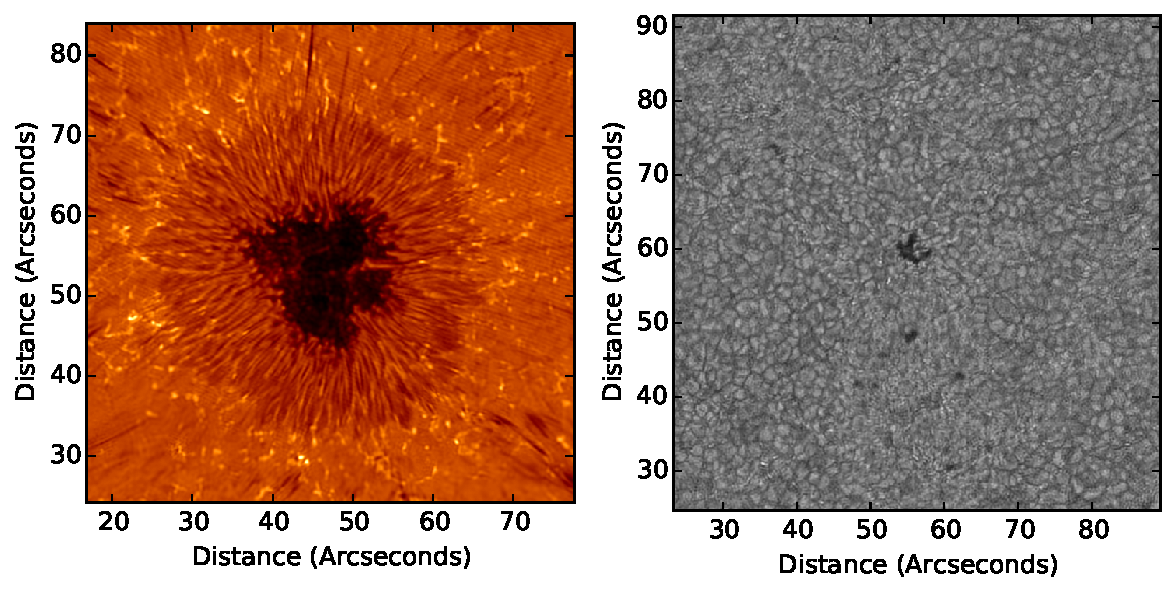
\includegraphics[width=\textwidth]{overview.pdf}
		\caption
		{
		An overview of the field-of-view (FOV) inferred by SST/CRISP and SDO/AIA consisting of:\,(a) SDO/AIA $170$ nm, detailing the photosphere; (b) SST H$\alpha$ $656.28$ nm (line core) sampling the chromosphere; the  (c) SDO/AIA $30.4$ nm filter (TR); and the lower corona detailed by (d) SDO/AIA $17.1$ nm.
		The white line on each image represents the slit used to construct the time-distance diagrams plotted in Figure \ref{fft_slit}.
		The yellow and cyan lines outline each slit used to investigate UPW behaviour.
	    The yellow slits show where UPWs were observed and cyan slits show no UPWs.
		}
		\label{chap5:overview}
	\end{figure*}

	The analysis presented here is conducted on AR $11511$, which displayed a myriad of complex features during these observations.
	The ground-based data were obtained using the CRisp Imaging SpectroPolarimeter (CRISP \citealt{Scharmer2008}) instrument, situated at the Swedish 1-m Solar Telescope (SST), on the 22nd June 2012 between 07:23 UT and 08:28 UT, during a period of excellent seeing.
	These data have a high spatial resolution of around $0.2$\arcsecs\ ($1$\arcsecs\ $\approx$ 725 km) and a cadence of $2.2$ seconds, allowing the small-scale structures of the lower solar atmosphere to be resolved (diffraction-limited) using a narrow-band $0.0269$ nm H$\alpha$ filter centred on $656.28$ nm.
	H$\alpha$ line scans were returned for $-0.1032, -0.0774, 0$ and $0.1032$ nm
	Each frame captured by the SST/CRISP instrument sampled a $68$\arcsecs\ by $68$\arcsecs\ FOV close to the disc centre.
	The data were reconstructed using the {\it Multi-Object Multi-Frame Blind Deconvolution} (MOMFBD) technique, giving an overall cadence of $2.2$ seconds and a spatial resolution of 0.12\arcsecs\citep{Noort2005}.
	We followed the standard procedures in the reduction pipeline for CRISP data (\citet{2015A&A...573A..40D}) which includes the post-MOMFBD correction for differential stretching suggested by \citet{2012A&A...548A.114H}, also see \citet{2013ApJ...769...44S} for more details.

	Finally, co-aligned highly ionised plasma comprising the upper solar atmosphere was observed using the Solar Dynamics Observatory's (SDO) Atmospheric Imaging Assembly (AIA) instrument at a spatial resolution of approximately $1.5$\arcsecs\ and a temporal resolution of $12$ seconds.

	In Figure \ref{chap5:overview}, we include a general overview of the FOV analysed here, taken at 07:23 UT.
	The pore of primary interest is located at approximately [123\arcsecs, 203\arcsecs] in helioprojective coordinates, and can be easily identified as it is situated underneath the overlaid cyan star symbol.
	Four images sampled at different heights in the atmosphere are included to give an impression of the three-dimensional structuring evident in this region.
	The photosphere and chromosphere are sampled by the SDO/AIA $170$ nm filter (Figure \ref{chap5:overview}a) and the SST/CRISP H$\alpha$ line core (Figure \ref{chap5:overview}b), respectively.
	The dynamic fibril events which appear to protrude away from the large pore in the H$\alpha$ line core, obscure the majority of the large-scale structuring (such as the network) observed within the photosphere.
	Only in regions where strong vertical magnetic fields are present, such as within the confines of the large pore, does any evidence of the photospheric structuring penetrate into the chromosphere.
	Finally, the TR and corona are observed through the SDO/AIA $30.4$ nm (Figure \ref{chap5:overview}c) and $17.1$ nm (Figure \ref{chap5:overview}d) filters.
	It should be noted that two small pores are also within the FOV, situated at approximately  [123\arcsecs, 215\arcsecs], however, they are not evident in the H$\alpha$ line core.

\section{Results and discussion}
\label{sect2}

\subsection{The observed Active Region}

	\begin{figure*}
		\centering
		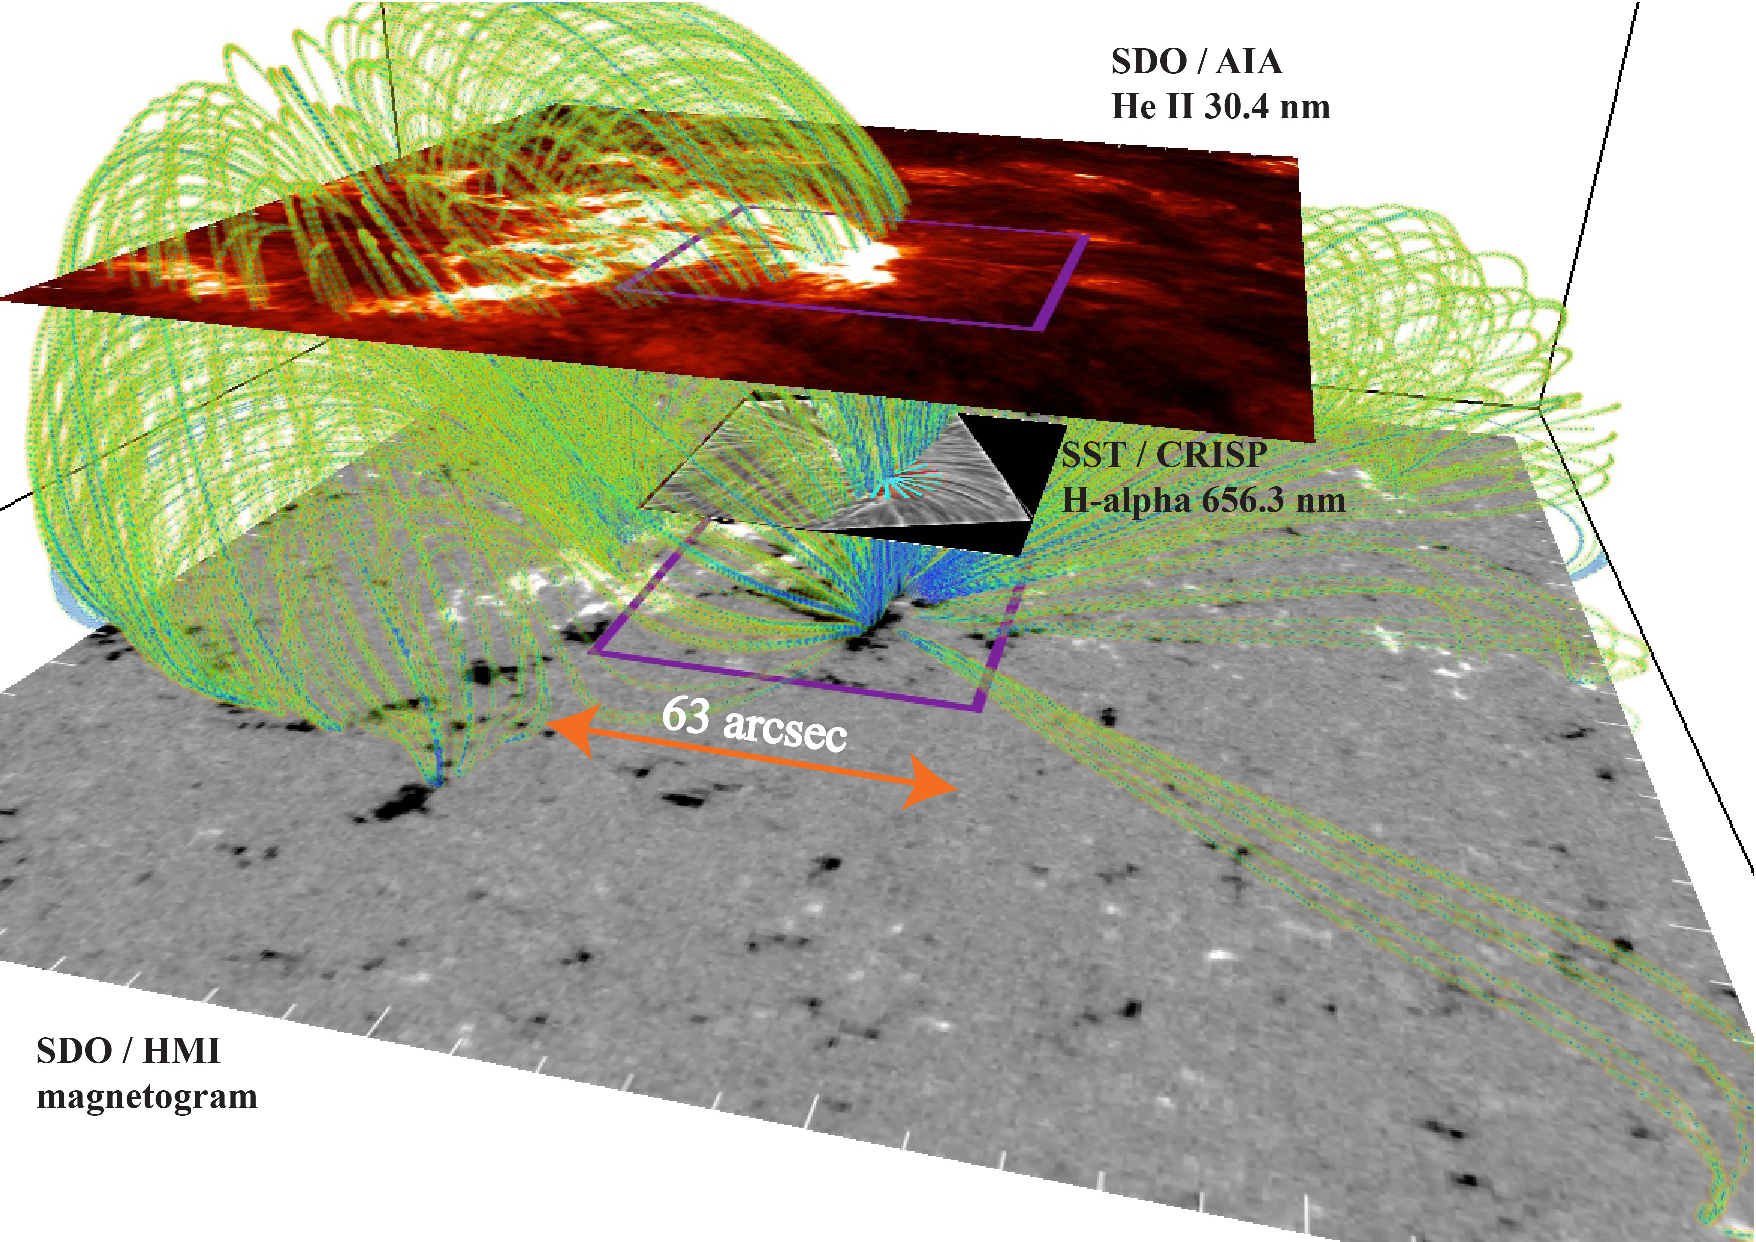
\includegraphics[width=\textwidth]{full_overview.pdf}
		\caption
		{
		The base layer indicates the magnetic field inferred by the SDO/HMI instrument.
		The purple box highlights the SST/CRISP FOV which is overlaid.
		An extended FOV context image from the SDO/AIA $30.4$ nm filter is also included.
		The green lines are the visualisation of the magnetic field extrapolation.
		A strong correlation exists between these lines and the brighter regions in the SDO/AIA $30.4$ nm image underpinning that the extrapolation is a reasonable approximation over such a large height.
		}
		\label{mag_field}
	\end{figure*}

	In Figure \ref{mag_field}, a stacked image outlining the counpling between the lower and upper regions of the solar atmosphere is presented.
	An extended FOV of the photospheric magnetic field is used as the base (with the SST/CRISP FOV overlaid as the purple box), from which the extrapolated field lines are plotted.
	Co-aligned photospheric magnetic field data were inferred by the SDO's Helioseismic and Magnetic Imager (HMI) instrument at a spatial resolution of around $1$\arcsecs\ and a cadence of $45$ seconds.
	Extrapolations of the magnetic field were then achieved by passing these data into the MPole Interactive Data Language package \citep{Longcope1996,Longcope2002}.

	We use MPOLE to determine the 3D coronal magnetic field line connectivity about the FOV as observed by CRISP. MPOLE implements the Magnetic Charge Topology models and the Minimum Current Corona model  to derive the coronal field from a set of point charges. In our analysis, the charges are an approximation of an observed photospheric magnetic field. The complete set of charge positions and strengths (fluxes) are contained as a set poles. The poles are extracted from the observations through applying a feature tracking algorithm to HMI magnetograms of the active region of interest (extended about the CRISP co-aligned FOV by 50 arcsec in both solar-\textit{x} and solar-\textit{y} directions). Feature tracking of regions of positive and negative flux is carried out using YAFTA (Yet Another Feature Tracking Algorithm \citealt{DeForest2007}). Poles are labelled features which are collections of pixels in the magnetogram that are grouped according to criterion such as, spatial size and magnetic field strength. Subsequently, pixels below a threshold in flux density are not grouped, and receive a zero label in the mask. The thresholds are employed to ensure a suitably representative distribution of the  magnetic flux concentrations of the active region of interest.

	It is immediately noticeable that a non-rotationally symmetric distribution of field lines is present.
	Over-laid the magnetic field, we stack concurrent images from the SST/CRISP H$\alpha$, SDO/AIA $30.4$ nm, and SDO/AIA $17.1$ nm filters.
	Typically, the formation heights of the H$\alpha$ line core is estimated to be around $1.5$ Mm, which agrees to the mid-chromosphere \citep{Leenaarts2007}.
	The SDO/AIA $30.4$ nm and $17.1$ nm filters correspond to plasma in the TR and low corona, while SDO/AIA $19.3$ nm and $21.1$ nm filters correspond to plasma in the corona/hot flare plasma and AR corona, respectively.
	The chromosphere shows many elongated dark and bright structures surrounding the pore, identified as fibrils.
	Furthermore, a bright moss-like region to the north of the pore is evident, which corresponds well with regions of high magnetic flux, identified by the extrapolation process.
	The associated magnetic field from the large pore is observed to penetrate into the chromosphere and potentially higher, and corresponds well with the regions of increased intensity within the $30.4$ nm and $17.1$ nm filters, supporting that this extrapolation is reasonable over such a large height.
	The umbra of the two smaller pores do not appear to penetrate into the chromosphere, most likely due to insufficient magnetic flux.
	It should be noted, however, that UPWs patterns are still seen to propagate above the location of the rightmost pore in the H$\alpha$ line core.
	This indicates that the magnetic field lines do still expand into the solar chromosphere.
	In the higher temperature filters, the clarity of the pore fades, and large-scale loop structures, co-spatial with the extrapolated field lines, can be found.
	On the opposite side of the pore, a region of lower emission is observed in the TR and coronal lines co-spatially with less vertically inclined field lines returned by the magnetic field extrapolation.
	In the following sections, we discuss the influence of the magnetic field topology on observations of UPWs within this AR.
	It is imperative to note, that the height of each stacked image in Figure \ref{mag_field} was estimated merely for ease of visualisation and should not, therefore, be used as strong evidence that the less vertically inclined field lines do not penetrate into the upper atmosphere.

\subsection{Upwardly Propagating Waves}

	\begin{sidewaysfigure}
		\centering
		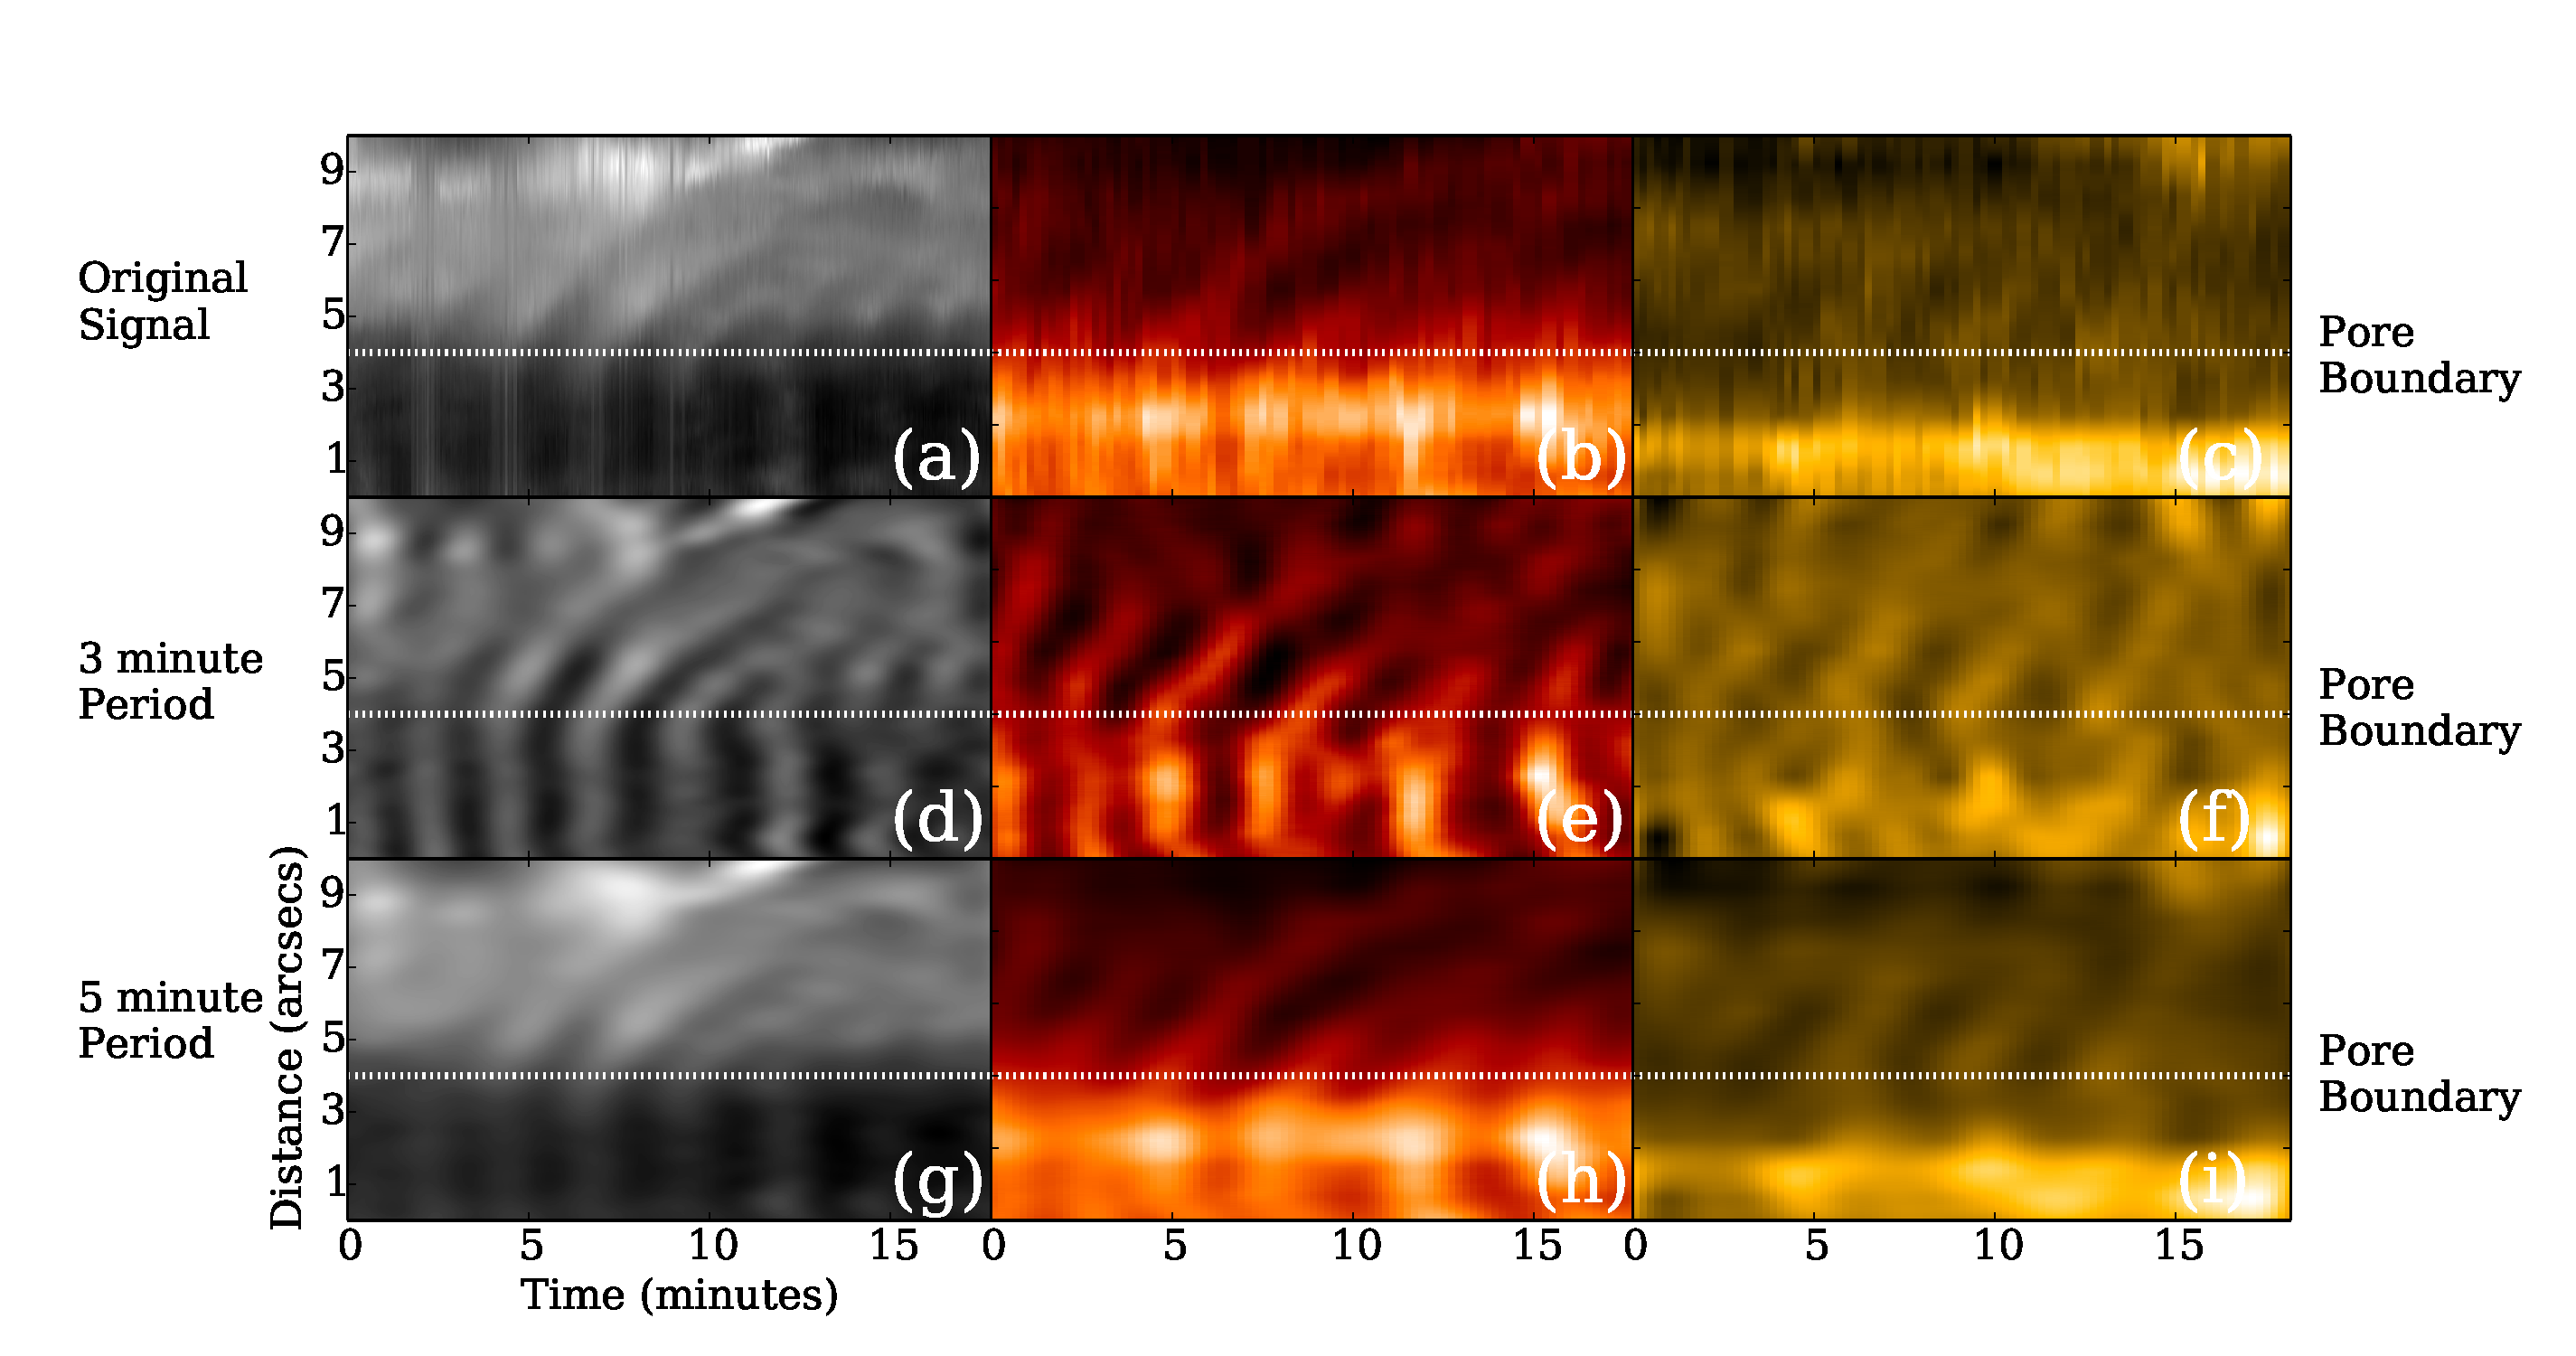
\includegraphics[width=\textwidth]{slits.pdf}
		\caption
		{
		(Top row) Unfiltered time-distance slits for the H$\alpha$ line core (a), SDO/AIA $30.4$ nm filter (b), and $17.1$ nm filter (c) constructed for the white slit in Figure \ref{chap5:overview}. (Middle row) Time-filtered 3-minute FFT output for H$\alpha$ (d), SDO/AIA $30.4$ nm (e), and SDO/AIA $17.1$ nm (f). (Bottom row) 5-minute FFT output for H$\alpha$ (g), SDO/AIA $30.4$ nm (h), and SDO/AIA $17.1$ nm (i).
		The windows used are centred on $3\pm1.5$ mHz (referred to as $5$ minutes) and $5\pm1.5$ mHz (referred to as $3$ minutes).
		The white dotted line is the pore boundary, below the line is the pore and above is the background chromosphere.
		}
		\label{fft_slit}
	\end{sidewaysfigure}

	The main focus of this chapter is the analysis of UPWs.
	These events manifest as dark wavefronts, easily identified against the H$\alpha$ background, which appear to propagate radially away from the large pore with a coverage angle of approximately $160\degree$.
	The coverage of the UPWs is inclusive of both unstructured (such as at the north of the pore) and highly structured regions (on the east of the pore), implying that no specific magnetic topology is required in the H$\alpha$ line core to facilitate the propagation of these waves.
	It is interesting to note, however, that no UPWs are observed to propagate either south or west from the pore during these observations, implying that a fundamental, but as of yet unknown, factor is limiting either the observation or propagation of waves in this region.
	A reason for the absence could be the inclination of the magnetic field (see Figure \ref{mag_field}) and will be expanded upon later in this Section.

	In Figure \ref{fft_slit}, we present a series of time-distance diagrams constructed using the white representative slit overlaid on Figure \ref{chap5:overview}.
	The top row of Figure \ref{fft_slit} plots the raw data extracted for this slit between 07:23:35 UT and 07:41:53 UT for the H$\alpha$ line core (a), the SDO/AIA $30.4$ nm filter (b), and the SDO/AIA $17.1$ nm filter (c).
	It should be noted that the start times for the SDO/AIA $30.4$ nm and $17.1$ nm filters are 9 seconds and 1 second ahead of the SST/CRISP data series, respectively.
	The UPWs are easily identified within the H$\alpha$ line core (as dark wavefronts) and the SDO/AIA $30.4$ nm filter (as bright wavefronts) propagating diagonally away from the pore between $3$\arcsecs\ and, approximately, $8$\arcsecs.
	The apparent horizontal velocity of the observed UPWs appears to decrease as the wavefront propagates away from the source.
	It has been hypothesised that the decrease in speed may be explained by ``the combined action of different frequency modes''\citep{UTMO}, i.e., that an UPW is a superposition of two or more waves with different frequencies.
	Within the representative H$\alpha$ slit, the detected UPWs slow from $17\pm0.5$ km s$^{-1}$ to $12\pm0.5$ km s$^{-1}$ at distances of $4$\arcsecs\ to $5$\arcsecs, respectively.
	To conclusively test whether the observed deceleration was a physical property of the waves or a product of using straight slits for analysis, we conducted further research of time-distance diagrams constructed using curved slits, which traced fibril 	structures within the H$\alpha$ line core.
	Due to the occurrence of this deceleration in each analysed slit, we conclude that this behaviour of a reduction in apparent velocity is indeed a property of UPWs.
	Intuitively, as only two factors, namely the actual velocity and the angle of propagation, are required to formulate the apparent velocity, we are able to tentatively suggest that we observe either a physical slow-down of the wavefront or a change in the angle of propagation of these waves.

	The spatial occurrence of these waves is a further interesting point which requires discussion.
	Through the analysis of each cyan slit highlighted in Figure \ref{chap5:overview}, investigation into how the behaviour of these waves changes spatially around the pore is feasible.
	At distances between $2$\arcsecs\ and $3$\arcsecs\ away from the pore boundary (indicated by the dashed white line in Figure \ref{fft_slit}) for each individual slit, the apparent phase speed ranges from $10$-$20$ km s$^{-1}$ (\textit{i.e.}, approximately the sound speed in the chromosphere).
	As UPWs are observed as single wavefronts, it is possible that the magnetic field topology is influencing the apparent horizontal velocity spatially around the pore.
	By overlaying the slits in which UPWs are observed onto the interpolated magnetic field, plotted in Figure \ref{mag_field}, we are able to infer a spatial correlation between the apparently less vertically inclined magnetic fields and the occurrence of UPWs.
	The observations of such non-radially symmetric wavefronts around a pore, guided by the magnetic field, suggests that the extension of the magnetic field into the solar atmosphere from the pore, is non-axially symmetric.
	This result poses an interesting question: Does a combination of viewing angle and magnetic field topology limit the potential detection of propagating UPWs around the magnetic waveguide?
	It is imperative that a future analysis, ideally combining observations and simulations, be undertaken to further test this.

    We now direct our investigation towards understanding the potential influence of different wave modes on the raw UPW signals.
	By employing the FFT technique on each row of the time-distance diagrams (Figure \ref{fft_slit}a-c), the $3$-minute period for each wavelength can be isolated from the general wave behaviour.
	The windows used are Gaussian shaped, centred on $3\pm1.5$ mHz (referred to as $5$ minutes) and $5\pm1.5$ mHz (referred to as $3$ minutes) with a width of 2 mHz.

	The second row of Figure \ref{fft_slit} depicts the result of such an analysis for the H$\alpha$ line core (d), the SDO/AIA $30.4$ nm filter (e), and the SDO/AIA $17.1$ nm filter (f).
	The H$\alpha$ $3$-minute component starts off within the pore as an umbral flash-like event and, then, as the wave enters the surrounding atmosphere, moves away at a near constant speed, comparable to the raw data.
	It is easy to identify, that within the H$\alpha$ line core $3$-minute slit, the contrast of the waves against the background is increased when compared to the raw data.
	This suggests that the $3$-minute mode provides a high proportion of the energy carried by UPWs around the pore.
	A similar behaviour is observed within the SDO/AIA $30.4$ nm wavelength, however, no signal is isolated within the SDO/AIA $17.1$ nm filter for this slit.
	Understanding these observations in terms of the physical properties of waves is essential to fully understand the UPW phenomena.
	Overall, the coverage angle, around the pore, of the $3$-minute mode within the SDO/AIA $17.1$ nm filter is approximately $50$ \% lower than the $30.4$ nm filter.
	The question as to whether this is a result of the waves not propagating into the $17.1$ nm passband or a reduced contrast against the background should lend itself to an interesting future study.

	\begin{figure*}
		\centering
		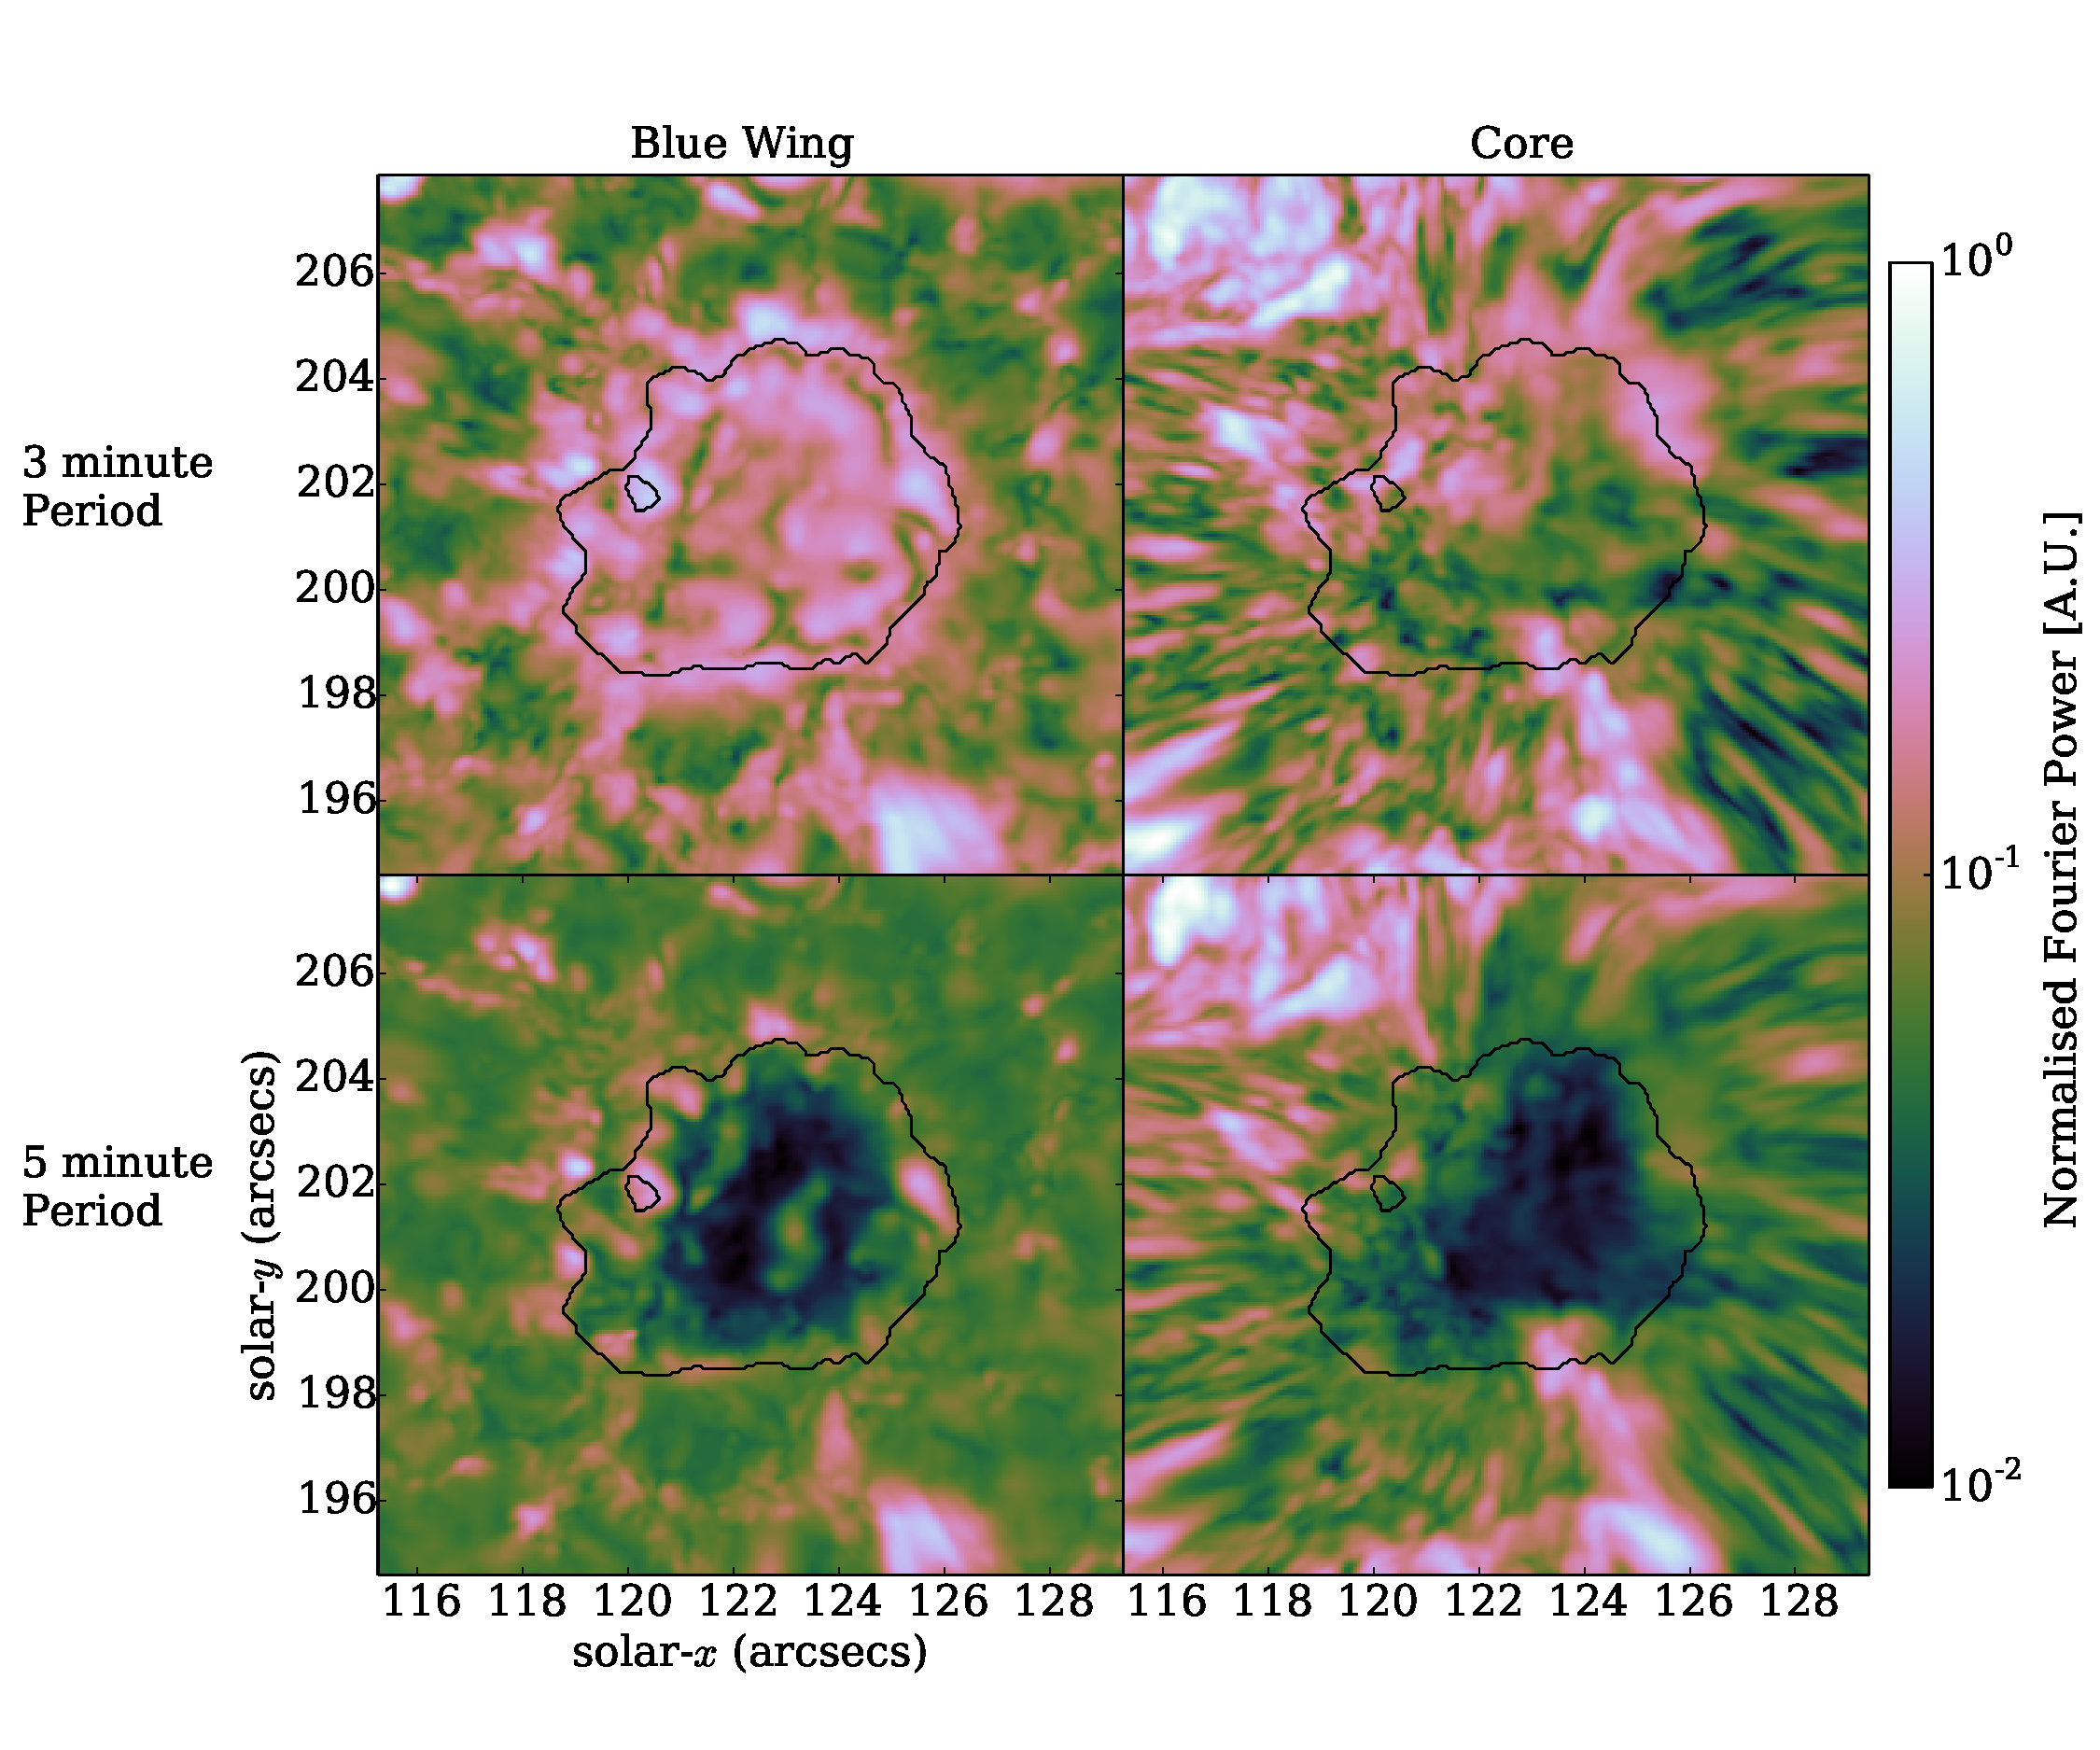
\includegraphics[width=\textwidth]{fft.pdf}
		\caption{
		The spatial distribution of normalised Fourier power of the LOS intensity with 3- and 5-minute filter windows.
		The black contour line highlights the pore boundary as observed within the H$\alpha$ line wings. We depict the:
		(a) 3-minute filtering of the H$\alpha$ wing;
		(b) 3-minute filtering of the H$\alpha$ core;
		(c) 5-minute filtering of the H$\alpha$ wing;
		(d) 5-minute filtering of the H$\alpha$ core.
		}
		\label{fft_power}
	\end{figure*}

	Analysis of the $5$-minute period (Figure \ref{fft_slit}g-i) allows for further inferences about the nature of these waves to be made.
	Within the H$\alpha$ line core, the occurrence of the $5$-minute mode is limited to regions outside of the pore, potentially due to the dependence of higher frequency modes on the magnetic field inclination\citep{DePontieu2004}.
	The phase speed is also reduced by approximately $1$-$2$ km s$^{-1}$ consistently around the pore.
	As there is more power within the $3$-minute mode close to the pore, it is assumed that this comprises the dominant component of the raw wavefront.
	It is possible, therefore, that the increased influence of the $5$-minute component as the wave moves away from the pore could explain the deceleration in raw phase speed, however, further research should be carried out to fully test this assertion.
	Within the SDO/AIA $17.1$ nm filter, the $5$-minute mode has a more defined wave pattern than the $3$-minute mode.
	We are, therefore, able to suggest that the $5$-minute mode more easily penetrates into the $17.1$ nm passband as has been suggested by previous researchers \citep{Moortel2002}, potentially providing energy into the TR.

	Another method that can be exploited to further understand the physical properties of these waves is a time-delay analysis.
	We were able to compare both the raw and FFT-filtered data for each wavelength in order to establish whether evidence of a lag exists.
	By taking into account the different start times for the SST/CRISP and SDO/AIA data, no observable lag was discernible.
	Therefore, we are able to conclude that either any lag between the signals is less than the cadence of these SDO/AIA data or that, indeed, no lag exists.
	Should the second hypothesis prove true, it would suggest that these observations support the propagation of a single wave, which occurs within the combined passbands of each of these filters, i.e., around the TR.

	By expanding the FFT analysis to the full FOV, we are able to analyse how power is manifested within the local plasma.
	Figure \ref{fft_power} shows the result of applying a $3$- and $5$-minute period FFT filter on the LOS intensity for the H$\alpha$ line core and far wing ($-0.1032$ nm).
	The same process was also applied to the concurrently taken SDO/AIA data, however, the obtained power maps lost their spatial structure and, as such, we were unable to make further conclusions.
	The black contour depicts the outline of the pore as observed in the photosphere sampled by the H$\alpha$ wing.
	Within the photosphere (Figure \ref{fft_power}a,c) the 3-minute power is isolated inside the pore structure; specifically, there appears to be large regions of power tracing the boundary of the pore, apparently analogous to the distribution of power within a sunspot \citep{Stangalini2012,Reznikova2012}.
	The power in the 5-minute band is minimal in the body of the pore but there is an increase at the pore-photosphere transition boundary corresponding to enhanced \textit{p}-mode power \citep{Mathew2008}.
    We interpret the confinement of the power within the pore as evidence that UPWs are driven by $p$-modes propagating vertically within the pore, which acts as a magnetic waveguide.

	Finally, we are able to analyse the H$\alpha$ line core.
	The increase of power especially within the 3-minute, easily observed to the north-east of the pore, corresponds well with the occurrence of UPWs within these data.
	It is intuitive to suggest that, as the FFT analysis is only applied in the vertical direction, the horizontal component of the UPWs in these regions limits the detection of power.
	Potentially, the increase in the FFT power observed to the north of the pore, could be indicative of the propagation of UPWs into the upper solar atmosphere along more vertically inclined magnetic field lines (as observed within Figure \ref{mag_field}).
	We interpret the lack of power co-spatially with the UPWs (in the east) as further evidence that the pore's magnetic field has become non-symmetric in the chromosphere.
	Evidence of the apparent dependence of both the observation of UPWs and the localised power within the plasma around a pore on the potential magnetic field topology, as presented within this chapter, is a key step in fully understanding the complex nature of coupling between layers of the solar atmosphere.

\subsection{Energy of UPWs}

	Following the identification and detailed analysis of UPWs around a pore, it is essential to estimate the potential energy carried by these waves into the upper solar atmosphere.
	Due to the decrease and increase in intensity in comparison to the background plasma for the H$\alpha$ line core and the SDO/AIA filters, respectively, it can be inferred that the wavefront represents an increase in density \citep{Allen1947,Leenaarts2012}.
	By measuring the contrast between the background plasma and the wavefronts, it is apparent that the intensity perturbations are within the linear regime and, therefore, these waves appear to be magneto-acoustic in nature.
	In order to further this analysis, we assume here that the lack of observed time-delay in these data implies that the lag is below the cadence of these data.
	Given estimated formation height-differences between the chromospheric H$\alpha$ line core and the SDO/AIA $30.4$ nm filter can be estimated to be around $0.5\pm0.25$ Mm, the upward propagation speed can be calculated as $42\pm21$ km s$^{-1}$.
	This speed is close to previous estimates of the fast speed in the chromosphere \citep{Morton2012}.
	It should be noted, that this corresponds well with previous results, which suggest that $p$-mode oscillations, which appear to drive these UPWs, are converted to fast modes \citep{Vigeesh2012}.
	The combination of these factors allows us to suggest that one of the most likely interpretations of these observations is that UPWs are {\it fast MHD sausage} waves.

	With the wave type being identified, it is now possible to calculate the estimated non-thermal energy for these waves.
	It is possible to estimate the energy flux at each pixel based on linearised MHD theory \citep[e.g.][]{Kitagawa2010}.
	The equation for the total energy flux of the fast MHD sausage wave is,
	\begin{equation}
		E_{wave} = \sum\limits_{i = 1}^{N}\rho_{0}[\tilde{I_{i}}/I_{0}]^{2}c_{ph}^{3},
		\label{energy}
	\end{equation}
	where $\tilde{I_{i}}$ is the intensity perturbation for each pixel, $I_{0}$ is the background intensity, $c_{ph}$ is the phase speed of the sausage wave, $\rho_{0}$ is the background density.
	We sum over each pixel which is part of the wave, giving us the average energy for that wave.
	Since the wave is a fast MHD sausage wave, the phase speed is $c_{fast}$ which is the local fast speed, however, since the ratio of the Alfv{\'e}n to the sound speed is $>>1$, the Alfv{\'e}n speed is the dominant value in the fast speed calculation.
	This assumes that the plasma is optically thin (intensity is proportional to density), which is true for the coronal lines however, not the case for H$\alpha$.

	This analysis leads to energy estimates of the order of $150$ W m$^{-2}$ for the wavefronts in the H$\alpha$ line core.
	These values drop by two orders of magnitude within the SDO/AIA filters.
	These energy flux values are about a factor of $100$ less than reported for other abundant sausage wave events in the chromosphere \citep{Morton2012}, however, they still comprise a important fraction of the energy flux required to heat the local quiet \citep{Wedemeyer2012} and active corona \citep{Aschwanden2007}, respectively.
	It should be noted, that these estimates are influenced by a number of observational factors, such as attenuation in the telescopic apparatus, changes in light levels throughout these data, and the angle of observation, to name a few.
	We do, however, suggest that during the period of these observations, there are approximately constant seeing conditions and, therefore, these energy estimates should be consistent.
	Magnetic pores cannot heat the entire corona, but can contribute to heating the local corona that is above and near the pore.
	The value for the energy flux is for the region where we can observe the UPWs and the most logical case is that UPWs occurs across the entire pore but are difficult to observe due to the local solar atmosphere.
	This should raise the value for the energy flux that has been obtained.

\section{Conclusions}
\label{sect3}

	The results presented in this chapter support the assertions that waves propagating radially away from concentrated magnetic waveguides (such as pores and sunspots) in the solar photosphere have significant vertical components that give rise to the illusion of horizontal propagation.
	The magnetic field reconstruction (as seen in Figure \ref{mag_field}) gives us a useful insight into the non-radially symmetric nature of this pore and, specifically, how the apparent topology of the magnetic field influences UPWs.
	The case that RPWs are in fact UPWs that travel along the field lines is mounting \citep{Bloomfiel2008,Jess2013}.
	Here, strong evidence is presented that energy from $p$-modes in the lower solar atmosphere travels directly upwards into the TR and lower corona.
	It has been reported that there is absorption of power at the boundary of the umbra-penumbra for a sunspot \citep[e.g.][]{Gosain2011}.
	Here, we observe enhanced power at the boundary of the pore at both three and  five minutes, while in the chromosphere, where UPWs are observed, there is a reduction of power.
	As the energy from the acoustic $p$-modes is converted into MHD waves along the flux tube, the period of the $p$-mode becomes three minutes and traces the magnetic field.
	When the wave travels into the TR and solar corona, there is decrease of the wave period.
	Rudimentary energy flux calculations reveal that these waves are able to contribute to heating the local corona, however, how much they contribute requires further study.

	From this primarily wave-based study of the solar atmosphere we deduce that, in the outside environment surrounding the pore, the magnetic field of the pore becomes non-symmetric.
	The non-symmetric magnetic field appears to be integral in allowing UPWs to be observed, however, whether these events occur in other regions around the pore but are undetected, requires further study.
	Further investigation is also required to fully assess whether the lack of UPW signal within some regions around the pore is a consequence of seeing or an, as of yet unascertained, physical property (such as the cut-off frequency).
	A possible interpretation of these waves is a singular wavefront observed in multiple pass bands, data from a wider range of sources should help answer these.
	This calls for an extensive investigation using detailed spectropolarimetry (ground-based) data to resolve the issue but also to determine the consequence of changing the LOS (i.e on the limb) on the observation of UPWs.
	We have shown that the complex lower solar atmosphere, which does act as a powerhouse in the heating of the outer atmosphere, can in fact be further understood through a purely wave-based investigation.

\graphicspath{{Chapter6/Figs/}}

\chapter{Conclusion}
\label{chapter6}
    
    \vspace*{\fill}\par
    \pagebreak

\section{Overview of the thesis}
    
	In this thesis, the results of two-dimensional image analysis of sunspots and magnetic pores in the lower solar atmosphere is detailed.
    These results are directly compared to theoretically derived results and indicate the ubiquitous presence of slow MHD sausage waves in the larger magnetic structures that inhabit the solar surface.
    
    In Chapter 2, the telescopes and their associated instruments that supplied the science ready data sets are described, along with brief data reduction details.
    Then the signal analysis methods used to determine the periods and phase difference were detailed.
    These being the Fast Fourier Transform (FFT), Wavelets and Empirical Mode Decomposition (EMD).
    Finally, the method used to measure the cross-sectional area and total intensity of the magnetic structures is examined.
    The reason for this is to understand what the effects of varying the sigma multiplier has on the results of the signal analysis, which is important before this method is used to analyse data sets.
    
    In Chapter 3, the cross-sectional area and total intensity is measured on two sunspots and one magnetic pore.
    By comparing the phase difference between the cross-sectional area and total intensity signals, which are calculated using the method described in Chapter 2.
    It was possible to find the ubiquitous presence of slow MHD sausage waves within these magnetic structures.
    This conclusion is reached because the measured phase difference was very close to 0$^\circ$, i.e., they were in phase.
    This is the signature of the slow MHD sausage wave within cylindrical magnetic flux tubes.
    
    In Chapter 4, the cross-sectional area and total intensity is calculated for two new magnetic pore data sets.
    The phase difference indicated that the oscillations are slow MHD sausage waves.
    The usage of magneto-seismology equations allowed the calculation of several properties of the detected oscillations within the two magnetic pores.
    These were, for example, the radial distance perturbation, radial velocity perturbation and magnetic field perturbations.
    The properties of these oscillations gave the impression of standing harmonics.
    However, it was possible to use magneto-seismology to demonstrate that these oscillations are in fact standing harmonics.
    This was accomplished by working out if density stratification or radial expansion of the flux can cause the observed period ratios.
    The calculated radial expansion was in good agreement with previous simulations and observations. 
    
    In Chapter 5, the focus shifted from analysing the cross-sectional of magnetic structures to the analysis of Running Penumbral Waves (RPWs) in a magnetic pore.
    RPWs have only observed in sunspot penumbras; however, RPW-like events were observed, for the first time, to occur around a magnetic pore.
    This observation is the final step in confirming that RPWs are a visual effect of MHD sausage waves following the curvature of magnetic field lines of sunspots and magnetic pores.
    These have been previously termed Upwardly Propagating Waves (UPWs).
    This visual effect is caused because the magnetic field becomes more radially inclined further from the umbral centre.
    These radially inclined fields have longer arc lengths and thus a wave following these field lines have to cover a larger distance before it can appear in the chromosphere.
    This creates a delay of the appearance of these waves at higher levels, causing this patten of radially outward propagating waves.
    These events are able to deliver a small amount of energy into the local corona, but not enough to heat the active corona.
       
\section{Summary of results}

	\subsection{Chapter 2}

    Chapter 2 started by detailing the various solar telescopes, space- and ground-based, utilised within this thesis.
    It covered the instruments that was either on board the space-based telescopes or attached to an optics bench for ground-based telescopes.
    From here, the three signal analysis methods employed are described: FFT, Wavelets and EMD.
    It detailed how each method works, strengths and weakness and why three methods were used instead of just one.
    
    The chapter finishes on a study of the principle method that is used to measure the cross-sectional area of the sunspots and magnetic pores analysed within this thesis.
    The motivation was to understand if the method output was heavily affected or dependent on the sigma multiplier value chosen.
    If this was the case, then this had to be known before this method could be used for any scientific analysis.    
    The sigma multiplier is a crucial factor as it will influence the end result, which is the cross-sectional area and total intensity signals.
    In order to undertake this study, high-quality ground-based data was used from the Dunn Solar Telescope (DST).
    The instruments used from the DST are the \textit{Interferometric Bidimensional Spectrometer} (IBIS) and the \textit{Rapid Oscillations in the Solar Atmosphere} (ROSA) instrument.
    There are two datasets, one for each instrument, with the telescope pointed at a sunspot and a magnetic pore for IBIS and ROSA, respectively.
    This can be seen in Figure \ref{fig:data_overview}.
    These two data sets are a good representative of the data sets studied within this thesis.
    
    The sigma (mean) value used came from a background box of quiet Sun, i.e., a region of the photosphere that contains no magnetic features.
    Once the sigma value is calculated, it is multiplied by a value which is called the sigma multiplier.  
    Both magnetic structures were contoured using a selection of sigma multipliers, 3, 3.5, 4, and 4.5 and 2, 2.5, 3, and 3.5 for the sunspot and magnetic pore respectively.
    These values correspond to the colours: blue, green, purple and orange.
    This contouring is displayed in Figure \ref{fig:method_overview}.
    The reason for difference in sigma multipliers between the sunspot and magnetic pore is due to the lack of a good quiet Sun region within the IBIS dataset.
    This is clearly seen in the top right histogram in Figure \ref{fig:method_overview}, where the returned distribution is skewed, and this had the result of increasing the sigma multipliers.
    
    The resultant cross-sectional area signals are analysed using the wavelet transform and this revealed a range of periods within these magnetic structures.
    For the IBIS sunspot, the range of sigma multipliers did not alter the periods found by the wavelet transform.
    What did vary was the wavelet power of the periods, as seen in Figure \ref{fig:sunspot_wavelet}. 
    The range of sigma multipliers return a threshold value that contours pixels which encompass the sunspot umbra and not the penumbra or background photosphere.
    This is why the sigma multiplier has little effect on the output in this case.
    For the ROSA magnetic pore, the difference in multipliers is more important.
    Figure \ref{fig:pore_wavelet} demonstrates that for the larger sigma multipliers, the smaller periods have disappeared from the wavelet transform. 
    This is because, the returned threshold value from the higher sigma multiplier under contours the magnetic pore.
    As a result, the returned cross-sectional signal is missing a large number of pixels, which can be seen by the signals at the top of Figure \ref{fig:pore_wavelet}.
    This could mean that only certain regions of the magnetic pore oscillate and might be possible to isolate those regions in a future work.
  
    The results can be summarised as the following.
    The best way to choose a sigma multiplier that will be used to create the threshold value, is to take into account the structures's intensity distribution.
    This way, choosing a sigma multiplier becomes more straightforward and more robust than choosing a threshold value as a percentage of the quiet Sun intensity.
    As long as the sigma multiplier is sane, then there will be nothing missed from the analysis.
    
    Finally, the phase difference or phase relations are used to identify the various waves modes and these are listed in Table \ref{tab:phase}.
    All three signal analysis methods offer the ability to calculate the phase of each signal and that allows the comparison of the cross-sectional area to the total intensity phase difference.
    For this analysis, the wavelet transform was used to check the phase difference between the cross-sectional area and total intensity.
    These can be seen in Figures \ref{fig:phase_sunspot} and \ref{fig:phase_pore} for the IBIS sunspot and ROSA magnetic pore, respectively.
    Overall, the periods show in phase behaviour within these two magnetic structures which indicates slow MHD sausage modes. 
    The cross-wavelet phase images show that there is no effect of the different sigma multipliers on wave mode identification.
    It should be noted that this study can be expanded upon which will be discussed later on. 
    
   	\subsection{Chapter 3}
    	
    Chapter 3 detailed the application of the method described previously in Chapter 2, to three magnetic structures: two sunspots and one magnetic pore.
    These are shown in Figure \ref{images}.
    These data sets came from two ground-based solar telescopes: the Dutch Open Telescope (DOT) and the Swedish Vacuum Solar Telescope (SVST). 
    These were described in Chapters 2 and 3 and while these telescopes are now out of service, they offered very decent data sets.
    
    Using a sigma multiplier of 2.5 to contour these magnetic structures, resulted in cross-sectional area and total intensity signals.
    Both the wavelet and EMD were employed to identify periods within these data sets and they revealed a range of periods within each magnetic structure's cross-sectional area and total intensity signals.
    These can be seen in Figures \ref{1999sunspot} and \ref{1999IMF}, \ref{2005sunspot} and \ref{20005IMF}, \ref{2008pore} and \ref{20008IMF}, for the sunspot observed with the SVST, the sunspot observed with the DOT and the magnetic pore observed with the DOT respectively.
    The periods found ranged from 2 to 40 minutes and many of the cross-sectional area periods had a corresponding total intensity period.
    Furthermore, a direct comparison of the cross-sectional area periods with line-of-sight (LOS) intensity oscillations found previously in sunspots demonstrates similar, if not the same, periods \cite{kobanov}.
    However, if they are linked or the same oscillation in a different form has yet to be established.
   
    The phase difference between the cross-sectional area and total intensity was calculated to be close to zero degrees, from both the wavelet and EMD analyses.
    Using the phase difference relations from Table \ref{tab:phase} indicates that the observed oscillations are slow MHD sausage waves. 
    This implies that there is a prevalent amount of slow MHD sausage waves in these magnetic structures which are located in the photosphere.
    In addition, there were small regions of out of phase and $\pm$45 degree behaviour.
    The out of phase behaviour indicates a fast MHD sausage waves, however this was not consistent and thus was ignored. 
    The $\pm$45 phase difference is more difficult to explain.
    While there is no current MHD theory that explains this phase difference, it has been shown that noise in a signal can cause the cross-wavelet phase to become shifted by $\pm$45 degrees \citep{2015A&A...579A..73M}.
    This would be one reason why the wavelet transform would need to be cross-checked with another signal analysis method.
    However, it should be noted that in \cite{2015A&A...579A..73M}, the signal to noise ratio is very low which is not generally the case with solar observations. 
    
    Finally, whether these oscillations are propagating or standing waves has and still is an open question. 
    Since it is not possible to distinguish between these propagating or standing waves using only the cross-sectional area and total intensity phase relations, it would require another observable.
    It has been previously suggested that these oscillations are standing oscillations.
    To this end, Table \ref{chap3:harm_table} lists the discovered periods and their corresponding period ratios, if these oscillations were harmonics.
    In order to calculate these period ratios, it was assumed that the largest period within that data set was the fundamental mode. 
    Furthermore, Table \ref{chap3:harm_table} lists the period ratios in the ideal homogeneous flux tube case.       
    Thus, by comparing these values to the observed period ratios, gives additional momentum, that these oscillations are standing harmonics; however, further investigation is required.
    
    \subsection{Chapter 4}
    	
    Chapter 4 expands on the previous work in Chapter 3 by studying two further magnetic pores.
    These two new data sets come from the DOT and the DST using the ROSA instrument, which offers an increase in resolution and a decrease in time cadence from the data sets studied in Chapter 3.
    These two data sets can be seen in Figure \ref{overview}.
    Again, the cross-sectional area and total intensity of each magnetic pore is calculated by the method previously used in Chapters 2 and 3. 
    Both magnetic pores display a collection of oscillations but due to the shorter length of these data sets, the maximum periods found were shorter.
    The periods range from 2 to 20 minutes and can be seen in Figures \ref{DOT_wls} and \ref{ROSA_wls}.     
    The phase difference between the cross-sectional area and total intensity signals show that these oscillations are slow MHD sausage waves.
    
    The extension within this chapter is utilisation of the perturbation amplitude of these oscillations.
    Using linear ideal MHD theory, it is possible to derive equations that will calculate the the ratio of magnetic field perturbation to the background magnetic field as well as the radial displacement and radial velocity perturbation of these oscillations.
    These are Equations \ref{eq:mag_area}, \ref{eq:area_rad}, and \ref{eq:rad_vel}, respectively. 
    To achieve this, the amplitude of the oscillations was required and the EMD was used to provide this.
    The IMFs returned from the EMD algorithm are known to return close to the actual amplitude of the original signal.
    To make sure this was accurate, these results were checked with the FFT and were within 10\% of each other.
	It should be noted that the wavelet transform can not be used to work out perturbation amplitudes.
	This is because the power spectrum is biased towards lower frequencies and thus must be normalised.
  
    For the DOT pore, the amplitudes for the cross-sectional area oscillations are $3.87\mathrm{x}10^5$, $3.61\mathrm{x}10^5$ and $5.90\mathrm{x}10^5$ km$^2$ for the oscillations with periods of 4.7, 8.5 and 20 minutes, respectively.
    The radial perturbation was calculated to be 37, 34, and 56 km and the radial velocity perturbation was calculated to be 0.82, 0.42, and 0.29 km s$^{-1}$.
    The obtained radial speeds are very sub-sonic, however, they are of order of observed horizontal flows around pores.
    Furthermore, the percentage change in the magnetic field was to be found 4-7\%\ which was found for another magnetic pore observed with DST/IBIS \citep{0004-637X-806-1-132}.
    To calculate the wavelength the phase speed of the wave needs to known.
    Due to previous MHD wave mode identification, the slow MHD sausage mode, the phase speed in a photospheric tube was calculated to be 5.2 km s$^{-1}$ using a background sunspot atmosphere model.
    Finally, the obtained estimate of the wavelength for these oscillations was $1269$ km, $2268$ km and $5319$ km.
       
	For the ROSA pore, the amplitudes for the cross-sectional area oscillations are $2.29\mathrm{x}10^5$, $2.45\mathrm{x}10^5$, and $3.87\mathrm{x}10^5$ km$^2$ for periods of 2-3, 5.5, and 10 minutes, respectively.
    The radial perturbation amplitude was calculated to be 69.1, 74.2, and 117 km and a radial velocity perturbation as 3.03, 1.41, and 1.23 km s$^{-1}$.
    The percentage change in the magnetic field was found to be  25-45\%.
    This change is several times the size of the DOT pore and should be measurable in future observations. 
    For this data set, there were no corresponding magnetograms and as a result, this effect could not be verified.
    These results suggests that the oscillation strength might be independent of the scale of the structure \citep{Dorotovic2014}. 
    Finally, the calculated wavelength was 540-810 km, 1485 km, and 2.2 Mm.
    A summary of these findings can be found in Tables \ref{tab:ampl} and \ref{tab:wavelength}.
      
    The calculated wavelengths are further evidence for standing harmonic oscillations within magnetic flux tubes in the photosphere.
    To show this, if the assumption that these are standing harmonics is taken, magneto-seismology can be used to prove or disprove this assumption.
    This is possible because magneto-seismology allows the calculation of two important background properties of magnetic flux tubes in this case.
    It should be noted that these flux tubes are photospheric flux tubes that start at the photosphere and end at the transition region.
    The first is density stratification, which is the ratio of the density at the top of the flux tube to the bottom of the flux tube.
    The second is the expansion factor ($\Gamma$), which is the ratio of the radius at the top of the flux tube to the bottom of the flux tube.
    These are Equations (\ref{den_strat}) and (\ref{mag_strat}) and the period ratio between the fundamental and first harmonic is the output value from these equations.
    Table \ref{harm_table} lists the period ratios of the observed oscillations for the two magnetic pores within this chapter.
    Furthermore, other period ratios are used from Chapter 3 for this analysis.

	For density stratification, three density models were used: VAL-III C, sunspot umbra and magnetic bright point.
	These came from \cite{1981ApJS...45..635V}, \cite{Maltby1986} and \cite{GFME13a,GFE14}, respectively.
	The resulting period ratio from these three models were 1.44, 1.38 and 1.41.
	This does not correspond well to the results presented in this chapter, but only for one previously reported result in Chapter 3.
	It can be concluded that density stratification does not seem to be applicable for these cases.

	For the expansion factor, Equation (\ref{mag_strat}) was solved for a range of expansion factors and plasma-$\beta$ values, which can be seen in Figure \ref{fig:harm}.
	For the results within this chapter, the flux tube has to expand four to six times to have a period ratio that is observed.
	This was compared to a number of numerical simulations that model these types of flux tubes and an observation of a coronal loop, which were in good agreement with these results, see \cite{khomenko,fedun2,fedun1} and \cite{2008A&A...489L..57K}.
	This creates a consistent image of standing harmonics that are supported between the photosphere and transition region within sunspots and magnetic pores.

	\subsection{Chapter 5}
    
    Chapter 5 shifts the focus from cross-sectional area analysis of sunspots and magnetic pores to the investigation of Running Penumbral Waves (RPWs).
    RPWs have been observed within sunspot penumbras since the 1970's as intensity fronts propagating radially outwards from the outer umbra into the penumbra, before disappearing at the penumbra photosphere boundary.
    To study RPWs, ground-based data from the Swedish Solar Telescope (SST) using the \textit{CRisp Imaging SpectroPolarimeter} (CRISP) instrument was combined with co-aligned and co-temporal data from the \textit{Atmospheric Imaging Assembly} (AIA) instrument on board the Solar Dynamics Observatory (SDO) satellite.
    An overview of the ground- and space-based data can be seen in Figure \ref{chap5:overview}.
    The focus was on a small Active Region (AR) containing two magnetic pores.
    The first magnetic pore had a light-bridge through the middle and it could not been seen in the chromosphere.
    The second magnetic pore was the focus for this observation and it was a larger magnetic pore that was seen clearly in the chromosphere. 
    Wideband and white light images from the SST and SDO, respectively, showed that these magnetic pores had no penumbral structure in the photosphere.
    
    By focusing on the chromosphere around the two magnetic pores, RPW-like events could be seen to emanate clearly from the larger magnetic pore.
    It was also noted that despite the smaller magnetic pore not being able to penetrate into the chromosphere, RPW-like waves could be seen to from the chromosphere above it. 
    To confirm if these were RPWs, a slit analysis was performed around the larger magnetic pore in order to find out the periodicity and speed of these RPWs.
    One example of the slit analysis can seen in Figure \ref{fft_slit} and the result of that slit analysis is as follows.
    The periodicity and speed of these RPW-like events are consistent with RPWs observed around sunspots.
    Furthermore, these events do not emanate concentrically around the magnetic pore as happens commonly with sunspots.
    The RPW-like events are confined to a small arc, the regions of the chromosphere which is not dominated with dynamic fibrils or large static fibrils, essentially the quiet chromosphere.
    It has been hypothesised that RPWs are an optical illusion caused by a delay in the appearance of MHD waves that travel along magnetic field lines and they have been termed Upwardly Propagating Waves (UPWs, \citealt{Bloomfiel2008}).
    If this was the case for the wave events observed here, understanding how the magnetic field behaviours around this magnetic pore is important. 
	Figure \ref{mag_field} shows the output of a magnetic field extrapolation code called MPole \citep{Longcope1996,Longcope2002}, which used magnetograms from \textit{Helioseismic and Magnetic Imager} (HMI) on board SDO as a source.
	It offers evidence that where the RPW-like events are observed, the magnetic field is significantly more radially inclined which is a requirement in order to observe RPWs if they are UPWs. 
	This result was the first direct imaging of RPWs in a magnetic pore in the H$\alpha$ line core and confirming that RPWs are in fact UPWs.
	 
	Furthermore, these UPWs are observed in two SDO/AIA (30.4 nm and 17.1 nm) lines that are formed in temperatures that correspond to the transition region and low corona.
	This suggests that UPWs are able to reach the hotter regions of the solar atmosphere, which is consistent as various MHD wave phenomena have been observed in the corona above sunspots previously. 
	Finally, it was found that the UPWs are most likely a superposition of MHD waves that have different dominant periods.
	This was found previously for RPWs observed around a sunspot \citep{Jess2013}. 
	
	As the understanding of RPWs increased, the identification of the wave type become important and the current literature indicates that these are slow magneto-acoustic waves \citep{Bloomfiel2008}.
	To identify the wave type for the UPWs observed in this chapter, the phase speed needs to be calculated.
	A time lag analysis between the H$\alpha$ slit and the SDO/AIA slits was attempted and returned a result of less than 12 seconds, i.e., the lag is less than the cadence of SDO/AIA.
	The best assumption that can be made is that the lag is at that cadence, 12 seconds.
	It should be noted that this lag could actually be zero seconds. 
	This would imply that H$\alpha$ and the two SDO/AIA lines have a temperature response, at least partially, within the same temperature range and thus the observation is of UPWs in three different wavelengths at the same time. 
	
	
	 
    This gives the low phase speed estimate, but the result suggests that the UPW phase speed is greater than the sound and Alfv\'en speed (assuming typical chromospheric physical values) which means it is a fast wave. 
    However, this is the first report that of a RPW/UPW as a fast mode.
    With the wave mode identified, the next was the calculation of the energy of the observed waves.
    The energy is calculated to be around 150 W m$^{-2}$, which is enough to heat the quiet Sun corona but not an active region corona.
    This value has been found by another study for cross-sectional area oscillations in the low chromosphere.
    So overall, these waves have a small but important contribution to corona heating.
    
\section{Future work and questions}
    
    
        For future, does this isolate the regions where the pore oscillations? 
        
      
      Further, this implies that for the current range of ground-based solar telescopes, that the limiting factor for cross-sectional area oscillations is the resolution.
      This resolution has been fixed for the past couple of years and until Daniel K. Inouye Solar Telescope (DKIST) data becomes available, the range of sigma multipliers can vary without fear of biasing the results. 
          
          
          potential cross talk between area and intensity is ignored. Pure intensity oscillation would result in area oscillation due to a fixed sigma threshold. brighter > larger area ; darker > smaller area
   
   why is this the case? What bias can be introduced due to lack of resolution?
   an area variation is measured - area is defined by contouring intensity - intensity variation is introduced by some waves - the very thing we are trying to measure - is there potential for cross-talk, how addressed?
   
   again - is there a possibility that the intensity variation leads to the "appearance of cross sectional variation.
   
   still not clear how resolution limits or influences the results. What would we expect to gain or see that we don't see now?
   
          
             
    With any body of work, there are always unanswered questions or gaps in knowledge that ideally should be filled.
    As such, this thesis does not offer a full view of MHD sausage waves in sunspots and magnetic pores.
    
    Firstly, in Chapter 2, the method used to contour the magnetic structures was analysed.
    However, it was limited to low lying photospheric wavelengths.
    This would be expanded to cover other wavelengths which sample up into the chromosphere. 
    Studying how the cross-sectional area oscillations change as a function of height would be an important next stage for this research.
    In order to map how the amplitudes change with height, if the phase difference varies and if detected periods at one height exist within another height.
    However, as one moves upwards in the solar atmosphere, the boundary between a magnetic structure and the background atmosphere becomes harder to distinguish, so the analysis in Chapter 2 would need to be refined with multiple heights to investigate any pitfalls with layered datasets.
    Further to this, the current range of ground-based and space-based solar data has approximately the same resolution and this limit will be around for another two years. 
    This is a problem since the results are inherently dependant on this as this fixes the lower limit of any observations, especially when it comes to detecting perturbations.
    With DKIST, as well as Solar-C, this limit will be reduced.
    Thus, attempting this analysis on solar data from the next generation of solar telescopes would be a future extension of this work. 
    Finally, in Chapter 4, the phase speed of the MHD wave was calculated from typical background properties.
    Thus, the results that came from that are determined by those properties. 
    Further work would ideally employ magneto-seismology in order to calculate the phase speed of the detected oscillations. 
    Normally, this is possible using multiple heights since a time lag could be calculated with this method, as the height between wavelengths is known approximately.
    However, research \citep{2015A&A...579A..73M} have been published that makes it possible to do this with only the amplitude of the oscillations.
    This would be a further extension to the work in Chapter 3 and 4.
    
    Secondly, Chapter 2 detailed the signal analysis methods employed within this thesis.
    While these methods were useful and achieved the overall goals for each chapter, the field of signal analysis is ever evolving.
    For example, the wavelet transform has had numerous papers published which extend the algorithm to account for power bias at lower periods \citep{liu2007rectification,veleda2012cross} as well as being able to discern if the signal is standing or propagating \citep{2008SoPh..248..395S}.
    The Empirical Mode Decomposition has been extended, adding a step to the method where it does an ensemble averages \citep{wu2009ensemble}, better methods to deal with the edge effects with the spline fit \citep{zeng2004simple} as well as improved stopping criterion \citep{huang2008review}.
    It is important that the methods used to analyse signals and extract phase relations and amplitudes be made robuster in order to be certain in the period, phase and amplitudes of any oscillations found.
    If magneto-seismology requires these quantities to calculate the background properties of flux tubes, it is vital that any signal analysis method used is as robust as possible. 
    
    Finally, the observed UPWs within the magnetic pore is an interesting avenue of wave research.
    Here, there are many questions that need to be answered.
    To start, this observation indicated that the UPW events were fast sausage modes needs to be squared with the current literature.
    Either the interpretation is correct and UPWs can be either fast or slow waves or the analysis is incorrect.
    Further ground-based observations of magnetic pores would need to be conducted in order to understand UPWs within these structures.
    The author is only aware that RPWs have been only observed in sunspots , is the difference in wave mode due to a difference between sunspots and magnetic pores? 
    Does the presence of the penumbra cause this or would it be that the plasma-$\beta$ varies in a pore differently such that mode conversion leads to a fast magnetic-acoustic wave instead of a slow magnetic-acoustic wave?
    In Chapter 5, the region where the waves were observed was a small region of quiet chromosphere.
    Does the surrounding chromospheric atmosphere dictate if UPWs can be observed?
    Generally, symmetrical sunspots display concentric and clear RPWs, is that due to the magnetic field topology of the sunspot being much stronger than a magnetic pore, thus the observation of UPWs allows us to infer the magnetic field topology around sunspots and magnetic pores?
    Finally, do UPWs have a common source with the LOS oscillations and cross-sectional area oscillations observed in these magnetic structures, or are they the same wave that can be observed in several different ways?
    Solar physics has a long way to go and so does the research presented within this Thesis.

% ********************************** Back Matter *******************************
% Backmatter should be commented out, if you are using appendices after References
%\backmatter

% ********************************** Bibliography ******************************
%\begin{spacing}{1}

% To use the conventional natbib style referencing
% Bibliography style previews: http://nodonn.tipido.net/bibstyle.php
% Reference styles: http://sites.stat.psu.edu/~surajit/present/bib.htm

\bibliographystyle{apalike} % use this to have URLs listed in References
\cleardoublepage
\bibliography{References/references} % Path to your References.bib file

% If you would like to use BibLaTeX for your references, pass `custombib' as
% an option in the document class. The location of 'reference.bib' should be
% specified in the preamble.tex file in the custombib section.
% Comment out the lines related to natbib above and uncomment the following line.

%\printbibliography[heading=bibintoc, title={References}]


%\end{spacing}

% ********************************** Appendices ********************************

\begin{appendices} % Using appendices environment for more functunality
%
\chapter{Mathematical derivation} 

\section*{Chapter 4}

In Chapter 4, the set of equations, Equations (\ref{eq:mom_r}), (\ref{eq:mom_z}), (\ref{eq:mag_r}), (\ref{eq:mag_z}), (\ref{eq:press1}), and (\ref{eq:den}), are the ideal MHD equations that describe linear magneto-acoustic wave motions and are repeated below,
\begin{align}
    &&\rho_0 \frac{\partial v_r}{\partial t}=-\frac{\partial}{\partial r}
    \left(p_1+\frac{B_0b_z}{\mu_0}\right)+\frac{B_0}{\mu_0}\frac{\partial b_r}{\partial z},
    \label{eq:apen_mom_r}\\
    &&\rho_0\frac{\partial v_z}{\partial t}=-\frac{\partial p_1}{\partial z},
    \label{eq:apen_mom_z}\\
    &&\frac{\partial b_r}{\partial t}=B_0\frac{\partial v_r}{\partial z},
    \label{eq:apen_mag_r}\\
    &&\frac{\partial b_z}{\partial t}=-B_0\frac{1}{r}\frac{\partial (rv_r)}{\partial r},\\
    &&\frac{\partial p_1}{\partial t}=-\rho_0
    c_s^2\left(\frac{1}{r}\frac{\partial(rv_r)}{\partial r}+\frac{\partial v_z}{\partial z}\right),
    \label{eq:apen_press1}\\
    &&\frac{\partial \rho_1}{\partial t}=-\rho_0\left(\frac{1}{r}\frac{\partial (rv_r)}{\partial r}+\frac{\partial v_z}{\partial z}\right).
    \label{eq:apen_den}
\end{align}

Here, $p$ is the gas pressure, $\rho$ is the density and $\textbf{b} = (b_r,b_{\theta},b_z)$ is the perturbed magnetic field.
We have assumed that the plasma motion is adiabatic.
The subscripts $0$ and $1$ refer to unperturbed and perturbed states, respectively.
The velocity perturbation is denoted as $\textbf{v}_1= (v_r, v_{\theta}, v_z)$.

We will assume that all the perturbed quantities have the form of a harmonic propagating wave, $v_r=\hat{v_r}\cos(kz-\omega t)$, where $\hat{v_r}$ is the amplitude of the perturbation and is a function of the radius, i.e., $A(r)$.
With this information, it is possible to derive Equations (\ref{eq:n0}), (\ref{eq:n1}), (\ref{eq:n2}), (\ref{eq:n3}), (\ref{eq:n4}) and (\ref{eq:n5}).

To start, we can substitute the radial velocity perturbation into Equation (\ref{eq:mag_r}) or (\ref{eq:apen_mag_r}) giving,
\begin{align}
	&&\omega \hat{b_r} \cancel{\sin(kz-\omega t)} = -B_0k\hat{v_r} \cancel{\sin(kz-\omega t)}\\
	&&\omega \hat{b_r}= -B_0k\hat{v_r},\label{eq:brhat}\\
	&&\omega b_r=-B_0k\hat{v_r}\cos(kz-\omega t),\\
	&&\omega b_r=-B_0k{v_r},
\end{align}
which is Equation (\ref{eq:n0}).

Next we can substitute the radial velocity perturbation into Equation (\ref{eq:mom_r}) or (\ref{eq:apen_mom_r}) giving,
\begin{align}
    &&\rho_0 \omega \hat{v_r} \sin(kz-\omega t) =-\frac{\partial}{\partial r}
    \left(p_1+\frac{B_0b_z}{\mu_0}\right)+\frac{B_0}{\mu_0}\left(-\hat{b_r}k\sin(kz-\omega t)\right),\\
    &&\left(\rho_0 \omega \hat{v_r} + \frac{B_0}{\mu_0}\hat{b_r}k \right)\sin(kz-\omega t) =-\frac{\partial}{\partial r}\left(p_1+\frac{B_0b_z}{\mu_0}\right).\label{eq:apex_stepa}
\end{align}
As we know that $\hat{v_r} = A(r)$, and using Equation (\ref{eq:brhat}), we know that $\hat{b_r} = -\dfrac{B_0 k}{\omega}A(r)$, substituting these into Equation (\ref{eq:apex_stepa}) gives,
\begin{align}
&&\left(\rho_0 \omega A(r) - \frac{B_0^2 k^2}{\mu_0 \omega}A(r) \right)\sin(kz-\omega t) =-\frac{\partial}{\partial r}\left(p_1+\frac{B_0b_z}{\mu_0}\right),\\
&&\rho_0 \left(\frac{B_0^2 k^2}{\mu_0 \omega \rho_0} - \omega \right)A(r)\sin(kz-\omega t) =\frac{\partial}{\partial r}\left(p_1+\frac{B_0b_z}{\mu_0}\right),
\end{align}
and since $v_A^2 = \dfrac{B_0^2}{\mu_0\rho_0}$,
\begin{align}
&&\rho_0 \left(\frac{v_A^2 k^2}{\omega} - \omega \right)A(r)\sin(kz-\omega t) =\frac{\partial}{\partial r}\left(p_1+\frac{B_0b_z}{\mu_0}\right),
\end{align}
which is Equation (\ref{eq:n1}).

Equation (\ref{eq:mom_z}) or (\ref{eq:apen_mom_z}) is the same as Equation (\ref{eq:n2}), so no further work is required.

If we integrate Equation (\ref{eq:mag_r}) or (\ref{eq:apen_mag_r}), with respect to time,
\begin{align}
&&\frac{\partial b_z}{\partial t}=-B_0\frac{1}{r}\frac{\partial (rv_r)}{\partial r},\\
&& b_z = \int -B_0\frac{1}{r}\frac{\partial (rv_r)}{\partial r} dt,\\
&& b_z =  -\frac{B_0}{r}\int\frac{\partial (rA(r)\cos(kz-\omega t))}{\partial r} dt,\\
&& b_z =  -\frac{B_0}{r}\frac{\partial (rA(r))}{\partial r}\int \cos(kz-\omega t) dt,\\
&& b_z =  -\frac{B_0}{r}\frac{\partial (rA(r))}{\partial r}\left(\frac{-1}{\omega}\right) \sin(kz-\omega t) dt,\\
&& b_z =  \frac{B_0}{r\omega}\frac{\partial (rA(r))}{\partial r}\sin(kz-\omega t) dt,
\end{align}
which is Equation (\ref{eq:n3}).

Next, using Equations (\ref{eq:press1}) and (\ref{eq:den}) or Equations (\ref{eq:apen_press1}) and (\ref{eq:apen_den}) and multiplying Equation (\ref{eq:den}) or (\ref{eq:apen_den}) by $c_s^2$, it can be shown that,
\begin{align}
&&\frac{\partial p_1}{\partial t}=c_s^2\frac{\partial\rho_1}{\partial t}=-\rho_0 c_s^2\left(\frac{1}{r}\frac{\partial(rv_r)}{\partial r}+\frac{\partial v_z}{\partial z}\right)\label{eq:apen_n4},
\end{align}
which is Equation (\ref{eq:n4}).

Finally, integrating Equation (\ref{eq:n4}) or (\ref{eq:apen_n4}) with respect to time gives,
\begin{align}
&& p_1 =c_s^2\,\rho_1 = \frac{-\rho_0 c_s^2}{r} \int \frac{\partial(rv_r)}{\partial r} dt - \rho_0 c_s^2 \int \frac{\partial v_z}{\partial z} dt, \\
&& =\frac{-\rho_0 c_s^2}{r} \int \frac{\partial(r(A(r))\cos(kz-\omega t))}{\partial r} dt - \rho_0 c_s^2 \int \frac{\partial v_z}{\partial z} dt, \\
&& =\frac{-\rho_0 c_s^2}{r} \frac{\partial(r(A(r))}{\partial r} \int \cos(kz-\omega t)) dt - \rho_0 c_s^2 \int \frac{\partial v_z}{\partial z} dt.\label{eq:apen_part_2}
\end{align}
Integrating Equation (\ref{eq:n2}) with respect to time gives, $$v_z = \int -\frac{1}{\rho} \frac{\partial p_1}{\partial z} dt,$$ and then substituting this into Equation (\ref{eq:apen_part_2}) gives,
\begin{align}
&& p_1 = c_s^2\,\rho_1 =\frac{\rho_0 c_s^2}{r\omega}\frac{\partial(r(A(r))}{\partial r} \sin(kz-\omega t) + \frac{\cancel{\rho_0} c_s^2}{\cancel{\rho_0}} \int \frac{\partial}{\partial z} \left(\int \frac{\partial p_1}{\partial z} dt \right) dt,\\
&& = \frac{\rho_0 c_s^2}{r\omega}\frac{\partial(r(A(r))}{\partial r} \sin(kz-\omega t)  + c_s^2 \int\int \frac{\partial^2 p_1}{\partial z^2} dt dt.\label{eq:apen_wow}
\end{align}

If we let the pressure and density perturbations to be of the form, $p_1=\hat{p_1}\mathrm{q}(kz-\omega t)$ and $\rho_1=\hat{\rho_1}\mathrm{q}(kz-\omega t)$, respectively, where $\mathrm{q}$ is representative of a harmonic wave, i.e., it could be $\cos$, $\sin$ or some combination, for example, $\mathrm{q} = a \sin(kz-\omega t) + b \cos(kz-\omega t)$.
Then the right most term of Equation (\ref{eq:apen_wow}) will become,
\begin{align}
&&\int\int \frac{\partial^2 \mathrm{q}}{\partial z^2} dt dt,\\
&&\frac{\partial^2 q}{\partial z^2} = - k^2 \mathrm{q},\\
&&\int\int - k^2 \mathrm{q} dt dt = \frac{k^2}{\omega^2}\mathrm{q}.
\end{align}
This is because of the following,
\begin{align}
&&\frac{\partial^2 \sin(kz-\omega t)}{\partial z^2} = -k^2\sin(kz-\omega t),\\
&&\frac{\partial^2 \cos(kz-\omega t)}{\partial z^2} = -k^2\cos(kz-\omega t),\\
&&\int\int \sin(kz-\omega t) dt dt = -\frac{1}{\omega^2}\sin(kz-\omega t),\\
&&\int\int \cos(kz-\omega t) dt dt = -\frac{1}{\omega^2}\cos(kz-\omega t),
\end{align}
and this is still valid for any linear combination of these terms.

Thus Equation (\ref{eq:apen_wow}) will become,
\begin{align}
&& \hat{p_1}\mathrm{q} = \frac{\rho_0 c_s^2}{r\omega}\frac{\partial(r(A(r))}{\partial r} \sin(kz-\omega t) + \frac{c_s^2 k^2}{\omega^2}\hat{p_1}\mathrm{q},\\
&& \hat{p_1}\mathrm{q}\left(1 - \frac{c_s^2 k^2}{\omega^2} \right) = \frac{\rho_0 c_s^2}{r\omega}\frac{\partial(r(A(r))}{\partial r} \sin(kz-\omega t),\\
&& p_1\left(1 - \frac{c_s^2 k^2}{\omega^2} \right) = \frac{\rho_0 c_s^2}{r\omega}\frac{\partial(r(A(r))}{\partial r} \sin(kz-\omega t),\\
&& p_1 = \frac{\rho_0 c_s^2}{\frac{\omega}{\omega^2}(\omega^2- c_s^2k^2)}\frac{1}{r}\frac{\partial(r(A(r))}{\partial r} \sin(kz-\omega t),\\
&& p_1 = -\frac{\rho_0 c_s^2 \omega}{c_s^2k^2 - \omega^2}\frac{1}{r}\frac{\partial(r(A(r))}{\partial r} \sin(kz-\omega t),
\end{align}
which is Equation (\ref{eq:n5}).
%\include{Appendix2/appendix2}
%
\end{appendices}

% *************************************** Index ********************************
%\printthesisindex % If index is present

\end{document}
